\documentclass[12pt,a4paper]{report}

% Paquetes necesarios
\usepackage[T1]{fontenc}  % IMPORTANTE: T1 encoding para soporte de comillas
\usepackage[utf8]{inputenc}
\usepackage[spanish]{babel}
\addto\captionsspanish{\renewcommand{\tablename}{Tabla}}  % Cambiar "Cuadro" por "Tabla"
\usepackage{graphicx}
\usepackage{caption}  % Fix for captionof to prevent "figure" text appearing
\usepackage{geometry}
\usepackage{fancyhdr}
\usepackage{titlesec}
\usepackage{tocloft}
\usepackage{setspace}
\usepackage{hyperref}
\usepackage{amsmath}
\usepackage{amsfonts}
\usepackage{amssymb}
\usepackage{float}
\usepackage{xcolor}
\usepackage{tcolorbox}
\usepackage{listings}
\usepackage{tabularx}
\usepackage{booktabs}
\usepackage[section]{placeins}
\usepackage{needspace}
\numberwithin{figure}{section}
\renewcommand{\thefigure}{\thechapter.\thesection.\arabic{figure}}

% Aumentar espacio para números largos en lista de figuras
\setlength{\cftfignumwidth}{4em}

\usepackage{inconsolata}
\usepackage{url}
\usepackage{enumitem}  % Para listas personalizadas (glosario)
\usepackage{tikz}     % Para posicionar elementos sobre imágenes
\usepackage[expansion=false]{microtype}  % Desabilitar expansión de fuentes para evitar conflictos con inconsolata

\definecolor{codebg}{HTML}{FFFFFF}      % fondo blanco para impresión
\definecolor{codetext}{HTML}{000000}    % texto negro
\definecolor{codekeyword}{HTML}{0033CC} % azul oscuro para palabras clave
\definecolor{codestring}{HTML}{CC3300}  % rojo-marrón para strings
\definecolor{codecomment}{HTML}{008000} % verde oscuro para comentarios
\definecolor{codefunc}{HTML}{0066AA}    % azul para funciones
\definecolor{codeaccent}{HTML}{6600CC}  % púrpura oscuro para nombres especiales

\lstdefinestyle{angelcode}{
  backgroundcolor=\color{codebg},
  basicstyle=\ttfamily\small\color{codetext},
  keywordstyle=\color{codekeyword}\bfseries,
  commentstyle=\color{codecomment}\itshape,
  stringstyle=\color{codestring},
  emph={import,from,def,class,return,if,else,for,while,try,except,with,as},
  emphstyle={\color{codeaccent}\bfseries},
  showstringspaces=false,
  breaklines=true,
  breakatwhitespace=true,
  postbreak=\mbox{\textcolor{red}{$\hookrightarrow$}\space},
  prebreak=\raisebox{0ex}[0ex][0ex]{\ensuremath{\hookleftarrow}},
  frame=single,
  rulecolor=\color{black!40},
  frameround=tttt,
  framesep=6pt,
  aboveskip=1em,
  belowskip=1em,
  xleftmargin=0.5em,
  xrightmargin=0.5em,
  numbers=left,
  numberstyle=\tiny\color{black!50},
  upquote=true,
  columns=flexible,
  keepspaces=true,
  breakindent=20pt,
  breakautoindent=true,
  literate={"}{\textquotedbl}1
}
% Configuración de geometría
\geometry{
    left=3cm,
    right=2.5cm,
    top=2.5cm,
    bottom=2.5cm
}

% Configuración de interlineado
\onehalfspacing

% Configuración de hipervínculos
\hypersetup{
    colorlinks=true,
    linkcolor=black,
    citecolor=blue,
    urlcolor=blue,
    breaklinks=true
}

% Configuración de URLs para que siempre respeten márgenes
\urlstyle{same}
\def\UrlBreaks{\do\/\do-\do_\do.\do=\do?\do\&}
\Urlmuskip=0mu plus 1mu

% Configuración de títulos de capítulos
\titleformat{\chapter}[display]
{\normalfont\huge\bfseries}{\chaptertitlename\ \thechapter}{20pt}{\Huge}

% Configuración de encabezados y pies de página
\pagestyle{fancy}
\fancyhf{}
\fancyhead[L]{\small\nouppercase{\leftmark}}
\fancyhead[R]{\small\thepage}
\fancyfoot[C]{\small\nouppercase{\rightmark}}
\renewcommand{\headrulewidth}{0.4pt}
\renewcommand{\footrulewidth}{0.4pt}
\setlength{\headheight}{14.5pt}
\setlength{\footskip}{30pt}

\fancypagestyle{plain}{%
  \fancyhf{}
  \fancyhead[L]{\small\nouppercase{\leftmark}}
  \fancyhead[R]{\small\thepage}
  \fancyfoot[C]{\small\nouppercase{\rightmark}}
  \renewcommand{\headrulewidth}{0.4pt}
  \renewcommand{\footrulewidth}{0.4pt}
}

% Redefinir formato de marcas de capítulo y sección
\renewcommand{\chaptermark}[1]{\markboth{Capítulo \thechapter: #1}{}}
\renewcommand{\sectionmark}[1]{\markright{\thesection\ #1}}

% Forzar respeto de márgenes en todo el documento
\sloppy
\emergencystretch=3em
\tolerance=9999
\hyphenpenalty=10000
\exhyphenpenalty=10000

% Configuración del índice
\renewcommand{\cftchapleader}{\cftdotfill{\cftdotsep}}
\setcounter{tocdepth}{2}  % Mostrar hasta subsection en el índice (chapter=0, section=1, subsection=2)

\begin{document}

% Portada
\begin{titlepage}
    \centering
    \vspace*{0.5cm}
    
    % Logo/Imagen de portada (centrada arriba)
    
\includegraphics[width=0.6\textwidth]{imgs/portada.png}
    
    \vspace{1.5cm}
    
    % Universidad y Departamento
    {\Large \textbf{Universidad Tecnológica de la Mixteca}}\\[0.3cm]
    {\large Instituto de Computación}
    
    \vspace{2cm}
    
    % Título del documento
    {\LARGE \textbf{Marco Histórico y Referencial Para el Desarrollo de Aplicaciones con IA}}
    
    \vspace{2.5cm}
    
    % Presentado por
    {\large Presentado por:}\\[0.3cm]
    {\Large \textbf{José Ramón Aragón Toledo}}\\[0.5cm]
    {\large Matrícula: 2019020338}
    
    \vspace{1.5cm}
    
    % Carrera
    {\large Carrera:}\\[0.2cm]
    {\Large Ingeniería en Computación}
    
    \vspace{1.5cm}
    
    % Asesor
    {\large Asesor:}\\[0.2cm]
    {\Large M.C. Ricardo Ruiz Rodríguez}
    
    \vfill
    
    % Fecha
    {\large 27 de enero de 2026}
    
\end{titlepage}

% Contraportada - Imagen a página completa
\newpage
\thispagestyle{empty}
\newgeometry{margin=0pt}
\begin{tikzpicture}[remember picture,overlay]
    \node[anchor=center] at (current page.center) {%
        \includegraphics[width=\paperwidth,height=\paperheight,keepaspectratio=false]{imgs/contraportada.png}%
    };
\end{tikzpicture}
\restoregeometry
\newpage

% Índice General
{
\hypersetup{linkcolor=black}  % Links en negro para el índice
\tableofcontents
}
\clearpage

% ============================================================
% NOTA: RECURSOS DEL PROYECTO
% ============================================================
\chapter*{Recursos del Proyecto}
\addcontentsline{toc}{chapter}{Recursos del Proyecto}

\begin{center}
\fbox{%
\parbox{0.9\textwidth}{%
\centering
\vspace{0.3cm}
\textbf{\Large Material de Consulta y Código Fuente}

\vspace{0.5cm}

El código fuente completo de los proyectos \textbf{CharlesTherapy} y \textbf{Botas}, junto con todos los diagramas técnicos presentados en este documento, están disponibles públicamente en:

\vspace{0.3cm}

\textbf{\Large \url{https://github.com/Hudesde/JRATSS}}

\vspace{0.3cm}

\textbf{JRATSS} (\textit{José Ramón Aragón Toledo Servicio Social}) es un repositorio GitHub que alberga recursos relacionados con el desarrollo de aplicaciones basadas en inteligencia artificial, incluyendo implementaciones prácticas, diagramas técnicos y documentación detallada.

\vspace{0.3cm}

\hrule
\vspace{0.3cm}

\textbf{Contenido del repositorio:}

\begin{itemize}
    \item Código fuente de CharlesTherapy (Angular 19.2.0 + Express 5.1.0 + TypeScript 5.8.3 + MySQL 8.0.43)
    \item Código fuente de Botas (Perl 5.38 con 8 módulos + APIs de OpenAI)
    \item 5 diagramas técnicos PlantUML en formato PNG de alta resolución
    \item Archivos de configuración y dependencias
    \item README detallado con instrucciones de instalación y despliegue
    \item Ejemplos de uso y casos de prueba
\end{itemize}

\vspace{0.2cm}

\textit{Para cualquier duda, aclaración técnica o sugerencia sobre las implementaciones presentadas en este marco referencial, consulte directamente el material en el repositorio o abra un issue en GitHub.}

\vspace{0.3cm}
}%
}
\end{center}

\newpage

% Capítulo 1: Introducción
\chapter{Introducción}
\label{ch:introduccion}

En la actualidad, las Interfaces de Programación de Aplicaciones (API\textsuperscript{\hyperref[glos:api]{[G]}}, por sus siglas en inglés: \textit{Application Programming Interface}) orientadas al uso de modelos de lenguaje e inteligencia artificial\textsuperscript{\hyperref[glos:ia]{[G]}} representan un eje fundamental en el desarrollo tecnológico contemporáneo. Estas herramientas han modificado profundamente la manera en que las organizaciones automatizan procesos, analizan información y generan contenido de forma dinámica. Plataformas como OpenAI, Google o la más reciente DeepSeek\textsuperscript{\hyperref[glos:deepseek]{[G]}} han incorporado técnicas avanzadas de Procesamiento de Lenguaje Natural\textsuperscript{\hyperref[glos:pln]{[G]}} (NLP, \textit{Natural Language Processing}) y Aprendizaje Automático\textsuperscript{\hyperref[glos:ml]{[G]}} (ML, \textit{Machine Learning}), permitiendo que tanto instituciones como desarrolladores integren capacidades de razonamiento y generación de texto dentro de sus propias aplicaciones.

El presente documento tiene como propósito realizar un análisis comparativo entre dichas plataformas, considerando diversos aspectos técnicos y operativos, tales como la eficiencia computacional, la estructura de costos, la accesibilidad y los requerimientos de implementación. Este estudio no se limita únicamente a la utilización de APIs desde la perspectiva del consumidor, sino que también profundiza en sus posibles aplicaciones prácticas, tales como la generación de contenido personalizado, el análisis automatizado de documentos y la optimización de recursos informáticos.

Asimismo, se aborda la implementación de modelos de lenguaje de forma local mediante bibliotecas de Python, con énfasis particular en el caso de DeepSeek. Esta alternativa ofrece una vía más flexible y económica frente al consumo exclusivo de servicios en la nube, favoreciendo el control de la infraestructura y la personalización de los entornos de desarrollo. Desde esta perspectiva, el análisis busca ofrecer una visión integral que permita a empresas, investigadores y desarrolladores identificar la solución más adecuada según sus necesidades, equilibrando factores de innovación, presupuesto, escalabilidad y autarquía tecnológica.

\vspace{0.5cm}

\begin{tcolorbox}[colback=blue!5!white, colframe=blue!75!black, title=\textbf{Nota importante sobre recursos y material de consulta}]
Todas las implementaciones técnicas descritas en este documento (código fuente, diagramas, configuraciones) están disponibles públicamente en el repositorio GitHub del proyecto \textbf{JRATSS} (\textit{Just Resources And Technical Support System}):

\centering
\url{https://github.com/Hudesde/JRATSS}

\raggedright
\vspace{0.2cm}
Se recomienda consultar el repositorio para obtener detalles de implementación, archivos de configuración actualizados y ejemplos funcionales de los sistemas presentados.
\end{tcolorbox}

\vspace{0.5cm}

\section{Objetivos del proyecto}
\label{sec:objetivos}

El presente proyecto tiene como finalidad establecer un marco de referencia integral que permita comprender, comparar y aplicar de manera fundamentada las tecnologías de Inteligencia Artificial basadas en Modelos Grandes de Lenguaje\textsuperscript{\hyperref[glos:llm]{[G]}} (LLM, por sus siglas en inglés: \textit{Large Language Model}). A partir de esta premisa, se persiguen los siguientes objetivos específicos:

\begin{itemize}
    \item \textbf{Analizar el estado actual de las inteligencias artificiales generativas basadas en Modelos Grandes de Lenguaje (LLM).}  
    Examinar las tendencias recientes en el desarrollo de modelos de lenguaje y su impacto en la automatización de procesos cognitivos, la producción de contenido y la interacción humano–máquina.

    \item \textbf{Investigar las capacidades de los modelos con procesamiento multimodal.}  
    Explorar el grado de integración entre texto, imagen y otros tipos de datos, evaluando cómo los modelos más avanzados incorporan estas modalidades para mejorar la comprensión contextual y la generación de respuestas.

    \item \textbf{Examinar los modelos representativos del panorama actual.}  
    Estudiar las características técnicas, metodológicas y aplicativas de modelos como \textit{Gemini}\textsuperscript{\hyperref[glos:gemini]{[G]}}, \textit{ChatGPT}\textsuperscript{\hyperref[glos:chatgpt]{[G]}} (en su versión GPT-4V) y \textit{DeepSeek-R1-Distill-Qwen-7B}, valorando sus desempeños en tareas de generación y análisis de contenido multimodal.

    \item \textbf{Determinar la conveniencia de su uso.}  
    Identificar los beneficios, limitaciones y potenciales ámbitos de aplicación de estas herramientas, considerando parámetros como el rendimiento, la accesibilidad, el costo operativo y la adaptabilidad al contexto del usuario.

    \item \textbf{Establecer un marco de referencia para la utilización de APIs de inteligencia artificial.}  
    Proponer lineamientos para la integración práctica de estas tecnologías, con especial atención en la API de DeepSeek, mostrando su funcionamiento mediante ejemplos prácticos y aplicaciones con valor demostrativo.

    \item \textbf{Evaluar la viabilidad técnica de su implementación.}  
    Definir los requerimientos técnicos, bibliográficos y metodológicos necesarios para incorporar de manera efectiva estas soluciones en entornos propios, optimizando su desempeño conforme a las necesidades específicas del proyecto.
\end{itemize}


% Capítulo 2: Marco Teórico
\chapter{Marco Teórico}
\label{ch:marco_teórico}

Este capítulo inicia con una breve descripción de los conceptos fundamentales asociados a la Inteligencia Artificial en relación directa con los términos y acepciones comúnmente asociados en el uso de los Modelos Grandes de Lenguaje (LLM, por sus siglas en inglés: \textit{Large Language Model}), aspectos que resultan esenciales para contextualizar el desarrollo de este proyecto. Desde los paradigmas de aprendizaje automático hasta las arquitecturas neuronales que sustentan estos sistemas, cada elemento teórico contribuye a desentrañar el funcionamiento y las capacidades de herramientas que han transformado radicalmente la interacción entre humanos y máquinas.

\section{Métodos de aprendizaje en inteligencia artificial}
\label{sec:metodos_aprendizaje}

Los métodos de aprendizaje empleados en inteligencia artificial constituyen la base sobre la cual los modelos adquieren conocimiento a partir de los datos. Cada enfoque difiere en la forma en que se estructuran los datos de entrenamiento y en el tipo de supervisión aplicada durante el proceso de aprendizaje~\hyperref[ref:2.1]{[2.1]}.

\begin{center}
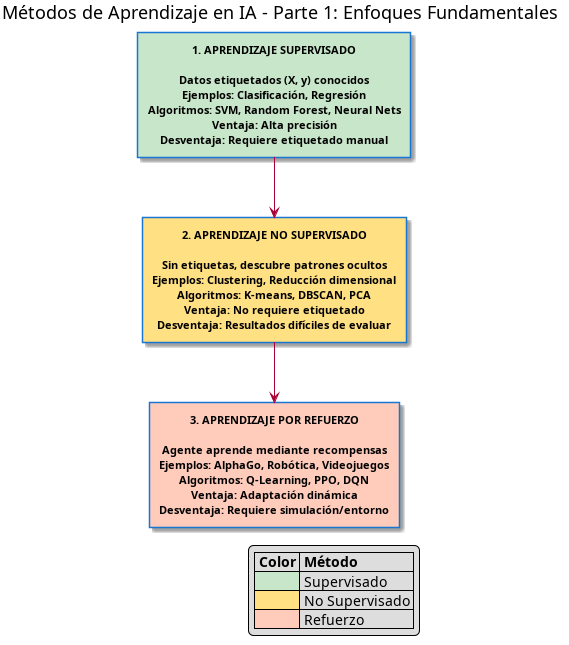
\includegraphics[width=0.68\textwidth]{imgs/infografias/metodos_aprendizaje_ia_parte1.png}
\captionof{figure}{Métodos fundamentales de aprendizaje en IA: supervisado, no supervisado y por refuerzo.}
\label{fig:metodos_aprendizaje_1}
\end{center}

\begin{center}
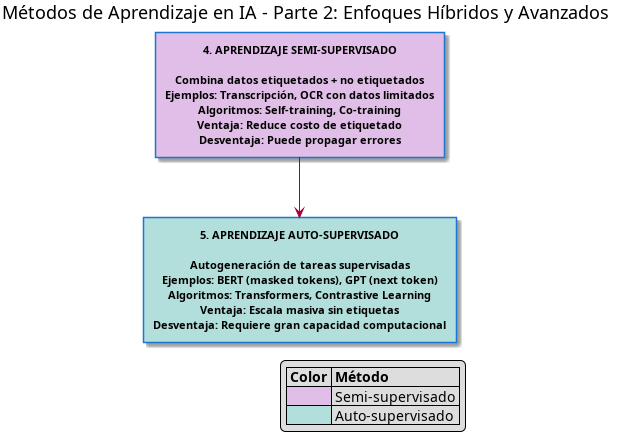
\includegraphics[width=0.68\textwidth]{imgs/infografias/metodos_aprendizaje_ia_parte2.png}
\captionof{figure}{Métodos híbridos y avanzados: semi-supervisado y auto-supervisado.}
\label{fig:metodos_aprendizaje_2}
\end{center}
\vspace{0.5em}

\begin{enumerate}
    \item \textbf{Aprendizaje supervisado.}  
    Se basa en el uso de datos etiquetados, donde el modelo aprende a asociar entradas con salidas previamente conocidas. Este método es ampliamente utilizado en tareas de clasificación y regresión.  
    \textit{Ejemplo representativo:} diagnóstico médico a partir de imágenes etiquetadas, como el sistema \textit{CheXNet}, desarrollado por investigadores de Stanford en 2017, capaz de detectar neumonía en radiografías de tórax con precisión comparable a radiólogos expertos. Para más información sobre CheXNet, consultar: \href{https://stanfordmlgroup.github.io/projects/chexnet/}{[Ver más]}.

    \item \textbf{Aprendizaje no supervisado.}  
    En este enfoque, el modelo analiza datos sin etiquetas para descubrir patrones, agrupamientos o estructuras subyacentes. Es común en la segmentación de clientes o la reducción de dimensionalidad.  
    \textit{Ejemplo representativo:} segmentación de clientes mediante el algoritmo \textit{K-means} aplicado a bases de datos de compras.

    \item \textbf{Aprendizaje por refuerzo.}  
    En este paradigma, un agente aprende a través de la interacción con un entorno, recibiendo recompensas o penalizaciones según sus acciones. Se utiliza con éxito en entornos de simulación y juegos complejos.  
    \textit{Ejemplo representativo:} el sistema \textit{AlphaGo}, desarrollado por DeepMind, que logró dominar el juego de Go mediante autoaprendizaje continuo (véase Sección~\ref{subsec:hitos_ia} para más detalles).

    \item \textbf{Aprendizaje semi-supervisado.}  
    Combina un conjunto reducido de datos etiquetados con una gran cantidad de datos sin etiquetar, mejorando la precisión sin depender de grandes volúmenes de anotaciones manuales.  
    \textit{Ejemplo representativo:} modelos de reconocimiento de voz que aprovechan grabaciones parcialmente etiquetadas.

    \item \textbf{Aprendizaje auto-supervisado.}  
    Este método permite al modelo generar sus propias etiquetas a partir de la estructura interna de los datos, sin requerir supervisión externa.  
    \textit{Ejemplo representativo:} modelos de lenguaje como \textit{BERT}\textsuperscript{\hyperref[glos:bert]{[G]}}, que aprenden a predecir palabras ocultas dentro de secuencias textuales~\hyperref[ref:2.1]{[2.1]}, \hyperref[ref:2.2]{[2.2]}, \hyperref[ref:2.3]{[2.3]}, \hyperref[ref:2.4]{[2.4]}.
\end{enumerate}

\section[Aplicaciones de la IA en la computación]{Aplicaciones de la inteligencia artificial en ramas de la computación}
\label{sec:aplicaciones_ia}

La inteligencia artificial ha revolucionado diversas áreas de la computación, introduciendo nuevas formas de optimizar procesos, automatizar análisis y desarrollar soluciones innovadoras. A continuación, se describen las principales aplicaciones documentadas en distintos campos~\hyperref[ref:3.1]{[3.1]}.

\begin{enumerate}
    \item \textbf{Ciencias de la Computación (Algoritmos y Teoría).}  
    Los algoritmos genéticos se aplican a la resolución de problemas de optimización complejos, como el \textbf{Problema del Agente Viajero} (también conocido como \textit{El Viajante} o TSP por sus siglas en inglés: \textit{Travelling Salesman Problem}), que consiste en encontrar la ruta más corta que permita a un vendedor visitar un conjunto de ciudades exactamente una vez y regresar al punto de origen ---un problema NP-completo clásico cuya complejidad crece factorialmente con el número de ciudades~\hyperref[ref:3.2]{[3.2]}. Asimismo, en las pruebas de software, el aprendizaje automático permite generar casos de prueba de manera automatizada, reduciendo significativamente el esfuerzo humano.

    \item \textbf{Ingeniería de Software.}  
    Los sistemas de generación de código asistidos por IA sugieren fragmentos de código en diversos lenguajes mediante análisis contextual~\hyperref[ref:3.3]{[3.3]}. Además, modelos especializados permiten identificar patrones de errores o vulnerabilidades en repositorios de software.

    \item \textbf{Bases de Datos.}  
    El aprendizaje automático contribuye a la optimización de consultas y a la elección de planes de ejecución más eficientes~\hyperref[ref:3.4]{[3.4]}. Algunos sistemas incorporan mecanismos predictivos para el mantenimiento automatizado y la detección de anomalías.

    \item \textbf{Redes de Computadoras.}  
    En las redes definidas por software, los algoritmos inteligentes optimizan el enrutamiento dinámico, mejorando la latencia y la estabilidad en redes 5G~\hyperref[ref:3.5]{[3.5]}. En materia de seguridad, los modelos de IA identifican patrones anómalos que indican posibles intrusiones.

    \item \textbf{Sistemas Embebidos e Internet de las Cosas (IoT).}  
    La computación en el borde (\textit{edge computing})\textsuperscript{\hyperref[glos:edgecomputing]{[G]}} posibilita la ejecución de modelos de visión por computadora en dispositivos con recursos limitados~\hyperref[ref:3.6]{[3.6]}. En entornos industriales, la robótica inteligente emplea aprendizaje automático para ajustar trayectorias con alta precisión.

    \item \textbf{Computación Gráfica y Visión por Computadora.}  
    Las redes neuronales convolucionales mejoran la calidad visual en tiempo real y facilitan la reconstrucción de imágenes~\hyperref[ref:3.7]{[3.7]}. Los modelos generativos, por su parte, son capaces de sintetizar imágenes coherentes a partir de descripciones textuales detalladas.

    \item \textbf{Seguridad en Cómputo.}  
    Los sistemas modernos de detección de malware se apoyan en clasificadores entrenados con aprendizaje supervisado~\hyperref[ref:3.8]{[3.8]}. De igual forma, los mecanismos de autenticación biométrica utilizan redes neuronales para el reconocimiento facial en dispositivos personales.

    \item \textbf{Computación Cuántica.}  
    En el ámbito de la computación cuántica, la IA se aplica a la corrección de errores en circuitos cuánticos, incrementando la estabilidad de los qubits~\hyperref[ref:3.9]{[3.9]}. Estudios recientes muestran el potencial del aprendizaje automático para optimizar operaciones y minimizar la decoherencia cuántica.
\end{enumerate}


\section[Contexto Histórico y Evolución de la IA]{Contexto Histórico y Evolución de la Inteligencia Artificial}
\label{sec:contexto_llms}

La comprensión cabal de los Modelos Grandes de Lenguaje exige situar su desarrollo dentro del devenir histórico de la Inteligencia Artificial como disciplina científica. Los LLM no constituyen un fenómeno aislado, sino la tecnología de vanguardia que emerge tras más de seis décadas de investigación, fracasos, reinvenciones y avances que han transformado la relación entre computación e inteligencia.

\subsection[Nacimiento de la disciplina (1943--1956)]{El nacimiento formal de la disciplina (1943--1956)}
\label{subsec:nacimiento_ia}

La Inteligencia Artificial surge formalmente en 1956 durante el célebre \textbf{Dartmouth Workshop}, organizado por \textbf{John McCarthy} ---quien acuñó el término ``Artificial Intelligence''---, \textbf{Marvin Minsky}, \textbf{Nathaniel Rochester} y \textbf{Claude Shannon}. La premisa fundacional, expresada en la propuesta original del taller, establecía que ``cualquier aspecto del aprendizaje o cualquier otra característica de la inteligencia puede, en principio, describirse con tal precisión que una máquina puede simularlo''.

\paragraph{Precursores intelectuales.}
Antes de Dartmouth, figuras seminales habían sentado las bases matemáticas y teóricas que harían posible la IA:
\begin{itemize}
    \item \textbf{Alan Turing} (1912--1954): En su artículo \textit{Computing Machinery and Intelligence} (1950), propuso el célebre \textbf{Test de Turing}\textsuperscript{\hyperref[glos:turing]{[G]}} como criterio operacional para evaluar la inteligencia de una máquina. Su trabajo previo sobre la máquina universal (1936) estableció los fundamentos de la computabilidad.
    
    \item \textbf{Claude Shannon} (1916--2001): Su \textit{Teoría Matemática de la Comunicación} (1948) formalizó conceptos como entropía, información y codificación, esenciales para el procesamiento de señales y, eventualmente, del lenguaje natural.
    
    \item \textbf{Norbert Wiener} (1894--1964): Fundador de la \textbf{Cibernética}, su obra de 1948 exploró los mecanismos de retroalimentación y control en sistemas biológicos y artificiales, anticipando conceptos centrales en el aprendizaje automático.
    
    \item \textbf{Warren McCulloch y Walter Pitts} (1943): Propusieron el primer modelo matemático de una neurona artificial\textsuperscript{\hyperref[glos:rna]{[G]}}, demostrando que redes de unidades simples podían, en principio, computar cualquier función lógica~\hyperref[ref:7.1]{[7.1]}, \hyperref[ref:7.2]{[7.2]}.
\end{itemize}

% =========================================================================
% SUBSECCIÓN INDEPENDIENTE: TEST DE TURING
% =========================================================================
\subsection[El Test de Turing]{El Test de Turing: Fundamento filosófico de la IA conversacional}
\label{subsec:test_turing}

El artículo \textit{Computing Machinery and Intelligence}, publicado por Alan Turing en la revista \textit{Mind} en octubre de 1950, representa uno de los textos fundacionales de la inteligencia artificial y, específicamente, de la IA conversacional que culminaría décadas después en los Modelos Grandes de Lenguaje.

\subsubsection{Contexto histórico y motivación}
\label{subsubsec:contexto_turing}

En 1950, las computadoras digitales apenas existían como concepto práctico. La supercomputadora \textbf{E.N.I.A.C.} (por sus siglas en inglés: \textit{Electronic Numerical Integrator and Computer}), construida en 1945, había demostrado la viabilidad del cálculo electrónico, pero la idea de que una máquina pudiera ``pensar'' parecía ciencia ficción. Turing, consciente de la carga filosófica de la pregunta ``¿Pueden las máquinas pensar?'', decidió reformularla en términos operacionales que evitaran debates interminables sobre la naturaleza de la consciencia.

\subsubsection{El Juego de la Imitación}
\label{subsubsec:juego_imitacion}

Turing propuso un experimento denominado \textbf{Juego de la Imitación} (\textit{Imitation Game}), estructurado de la siguiente manera:

\begin{enumerate}
    \item \textbf{Participantes}: Un interrogador humano (C), un humano (B) y una máquina (A), todos en habitaciones separadas.
    \item \textbf{Comunicación}: Exclusivamente mediante texto escrito (teletipos en la época; hoy, terminales de chat).
    \item \textbf{Objetivo del interrogador}: Determinar cuál participante es la máquina y cuál es humano.
    \item \textbf{Objetivo de la máquina}: Convencer al interrogador de que es humana.
    \item \textbf{Criterio de éxito}: Si el interrogador no puede distinguir consistentemente entre A y B, la máquina ``pasa'' el test.
\end{enumerate}

La elección del texto escrito como medio de comunicación fue deliberada: eliminaba señales no verbales (tono de voz, apariencia física) que podrían revelar la naturaleza artificial del participante, enfocando la evaluación exclusivamente en la \textbf{competencia lingüística y cognitiva}.

\subsubsection{Objeciones anticipadas por Turing}
\label{subsubsec:objeciones_turing}

En su artículo original, Turing anticipó y refutó nueve objeciones potenciales a su propuesta:

\begin{enumerate}
    \item \textbf{Objeción teológica}: ``El pensamiento es función del alma inmortal, que las máquinas no poseen.'' Turing respondió que Dios podría, si quisiera, otorgar alma a cualquier entidad.
    
    \item \textbf{Objeción ``cabeza en la arena''}: ``Las consecuencias de máquinas pensantes serían terribles, así que no pueden existir.'' Turing la descartó como irracional.
    
    \item \textbf{Objeción matemática}: Basada en los teoremas de incompletitud de Gödel, sugiere límites a lo que las máquinas pueden demostrar. Turing argumentó que los humanos también tienen limitaciones demostrables.
    
    \item \textbf{Argumento de la consciencia}: ``Solo quien experimenta consciencia puede pensar.'' Turing señaló que, llevado al extremo, este argumento conduce al solipsismo.
    
    \item \textbf{Argumento de las discapacidades}: ``Las máquinas nunca podrán X'' (enamorarse, escribir poesía, etc.). Turing cuestionó la base empírica de tales afirmaciones.
    
    \item \textbf{Objeción de Lady Lovelace}: Ada Lovelace afirmó que las máquinas ``solo hacen lo que se les ordena''. Turing argumentó que las máquinas podrían sorprendernos mediante comportamiento emergente.
    
    \item \textbf{Argumento de la continuidad del sistema nervioso}: El cerebro es analógico, las computadoras digitales. Turing demostró que sistemas digitales pueden aproximar comportamiento continuo arbitrariamente.
    
    \item \textbf{Argumento de la informalidad del comportamiento}: ``Las reglas no pueden capturar toda la conducta humana.'' Turing distinguió entre reglas de conducta y leyes de comportamiento.
    
    \item \textbf{Argumento de la percepción extrasensorial}: Turing, sorprendentemente, tomó en serio la posibilidad de telepatía, sugiriendo blindaje telepático para el test.
\end{enumerate}

\subsubsection[Funcionalismo vs. Consciencia]{Implicaciones filosóficas: Funcionalismo vs. Consciencia}
\label{subsubsec:funcionalismo}

El Test de Turing encarna una posición filosófica conocida como \textbf{funcionalismo}: lo que importa para atribuir inteligencia no es el sustrato material (neuronas vs.\ transistores), sino la \textbf{organización funcional} del sistema y su capacidad para producir comportamiento apropiado.

Esta postura contrasta con enfoques que exigen:
\begin{itemize}
    \item \textbf{Consciencia fenomenológica}: Experiencia subjetiva (``sentir algo'')
    \item \textbf{Intencionalidad genuina}: Estados mentales ``sobre'' algo (creencias, deseos)
    \item \textbf{Comprensión semántica}: No solo manipulación sintáctica de símbolos
\end{itemize}

El debate entre estas posiciones permanece abierto. Los Modelos Grandes de Lenguaje actuales exhiben comportamiento lingüístico sofisticado, pero si ``comprenden'' genuinamente o solo realizan predicción estadística de tokens sigue siendo una cuestión filosóficamente controvertida~\hyperref[ref:7.1]{[7.1]}, \hyperref[ref:7.2]{[7.2]}.

\subsubsection{Críticas posteriores al Test}
\label{subsubsec:criticas_turing}

A lo largo de las décadas, el Test de Turing ha recibido críticas sustanciales:

\begin{itemize}
    \item \textbf{Argumento de la Habitación China} (John Searle, 1980): Searle propuso un experimento mental donde una persona, sin saber chino, manipula símbolos siguiendo reglas y produce respuestas correctas en chino. Aunque ``pasa el test'', claramente no comprende chino. Conclusión: la simulación del comportamiento no implica comprensión genuina~\hyperref[ref:7.3]{[7.3]}.
    
    \item \textbf{Superficialidad conductual}: Programas como ELIZA (1966) y chatbots posteriores demostraron que trucos conversacionales pueden engañar a evaluadores sin inteligencia genuina.
    
    \item \textbf{Antropocentrismo}: El test privilegia inteligencia de tipo humano, excluyendo formas de inteligencia alternativas, especializadas o superiores en dominios específicos.
    
    \item \textbf{Dependencia del evaluador}: Los resultados varían según la sofisticación del interrogador y el tiempo disponible para la evaluación.
\end{itemize}

\subsubsection{El Premio Loebner y competencias modernas}
\label{subsubsec:premio_loebner}

En 1990, Hugh Loebner estableció el \textbf{Premio Loebner}, una competencia anual basada en el Test de Turing. Durante décadas, ningún programa logró convencer consistentemente a los jueces. Programas ganadores como \textbf{Eugene Goostman} (2014) ---que simulaba ser un adolescente ucraniano con inglés limitado--- generaron controversia sobre si representaban avances genuinos o simplemente explotaban expectativas reducidas.

La llegada de ChatGPT (2022) y modelos posteriores transformó radicalmente el panorama: por primera vez, sistemas de IA pueden mantener conversaciones extensas, coherentes y contextualmente apropiadas sobre prácticamente cualquier tema, aproximándose significativamente al criterio original de Turing~\hyperref[ref:5.1]{[5.1]}.

\subsubsection{Relevancia para los LLM contemporáneos}
\label{subsubsec:relevancia_llm}

El Test de Turing anticipó con notable precisión el desarrollo actual:

\begin{itemize}
    \item \textbf{Conversación como benchmark}: La capacidad conversacional sigue siendo el criterio primario de evaluación de chatbots y asistentes virtuales.
    
    \item \textbf{Texto como interfaz}: Turing eligió comunicación textual; los LLM operan fundamentalmente con texto.
    
    \item \textbf{Imitación como estrategia}: Los LLM aprenden a ``imitar'' texto humano mediante predicción del siguiente token.
    
    \item \textbf{Debates filosóficos persistentes}: ¿Comprenden los LLM o solo simulan comprensión? La pregunta de Turing sigue sin respuesta definitiva.
\end{itemize}

El legado de Turing trasciende el test específico: estableció que la \textbf{conversación en lenguaje natural} constituye un desafío central y un criterio de evaluación fundamental para la inteligencia artificial~\hyperref[ref:7.1]{[7.1]}, \hyperref[ref:7.2]{[7.2]}.

% =========================================================================
% SUBSECCIÓN: LAS TRES OLEADAS DE LA IA
% =========================================================================
\subsection[Las tres oleadas de la IA]{Las tres oleadas de la Inteligencia Artificial}
\label{subsec:tres_oleadas}

El desarrollo de la IA no ha sido lineal, sino cíclico, caracterizado por períodos de entusiasmo desmedido seguidos de ``inviernos'' de desencanto y recortes de financiamiento. La comprensión de estos ciclos resulta esencial para contextualizar el estado actual de la disciplina.

\begin{center}
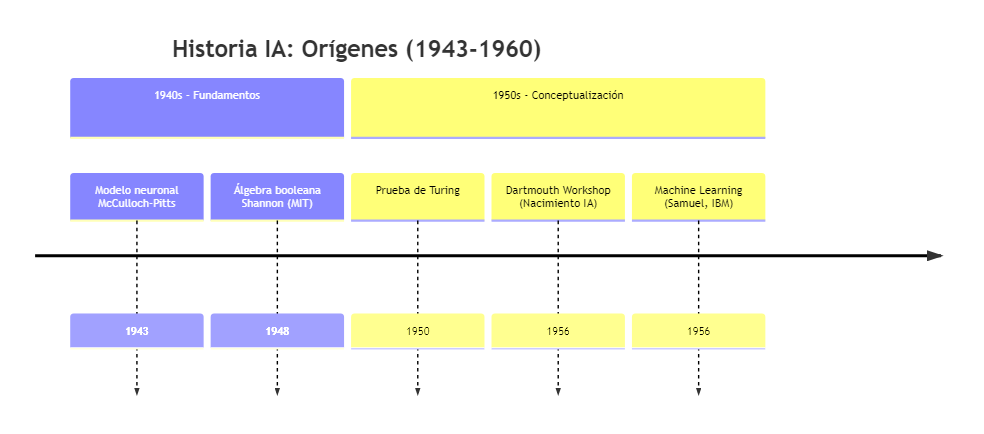
\includegraphics[width=0.95\textwidth]{documentation/06_timeline_llms/timeline_parte1_origenes.png}
\captionof{figure}{Línea temporal de la IA - Parte 1: Orígenes y fundamentos teóricos (1943--1956).}
\label{fig:timeline_origenes}
\end{center}
\vspace{0.5em}

\subsubsection{Primera oleada: IA Simbólica (1956--1974)}

La primera etapa de la IA estuvo dominada por el paradigma \textbf{simbólico} o \textbf{GOFAI} (\textit{Good Old-Fashioned AI}, término acuñado por el filósofo John Haugeland en 1985), fundamentado en la \textbf{Hipótesis de los Símbolos Físicos} de Newell y Simon (1976): la manipulación de símbolos mediante reglas lógicas constituye condición necesaria y suficiente para la inteligencia general. Este enfoque es históricamente relevante porque representó la primera aproximación sistemática a la IA, estableciendo fundamentos teóricos que influyeron en décadas de investigación ---aunque sus limitaciones eventualmente motivaron el surgimiento del conexionismo y el aprendizaje automático moderno.

\paragraph{Logros representativos.}
\begin{itemize}
    \item \textbf{STUDENT} (1964, Daniel Bobrow): Sistema capaz de resolver problemas algebraicos expresados en lenguaje natural, pionero en comprensión de lenguaje.
    
    \item \textbf{SHRDLU} (1970, Terry Winograd): Demostró comprensión y razonamiento sobre un ``mundo de bloques'' virtual mediante procesamiento de lenguaje natural~\hyperref[ref:7.3]{[7.3]}.
\end{itemize}

\subsubsection{ELIZA: El primer chatbot de la historia}
\label{subsubsec:eliza}

En 1966, Joseph Weizenbaum, investigador del Massachusetts Institute of Technology (MIT), desarrolló \textbf{ELIZA}\textsuperscript{\hyperref[glos:eliza]{[G]}}, considerado el primer programa informático capaz de simular una conversación en lenguaje natural. El sistema representó un hito en la historia de la interacción humano-computadora y sentó las bases de lo que hoy conocemos como \textit{chatbots}\textsuperscript{\hyperref[glos:chatbot]{[G]}}.

\paragraph{Arquitectura y funcionamiento.}
ELIZA operaba mediante un mecanismo relativamente simple de \textbf{coincidencia de patrones} (\textit{pattern matching}) y \textbf{sustitución de palabras clave}. El programa identificaba palabras o frases específicas en la entrada del usuario y aplicaba reglas de transformación predefinidas para generar respuestas. Por ejemplo:
\begin{itemize}
    \item Si el usuario escribía ``\textit{I am sad}'', ELIZA podía responder ``\textit{Why do you say you are sad?}''
    \item Frases con ``\textit{my mother}'' activaban preguntas como ``\textit{Tell me more about your family}''
    \item Cuando no encontraba patrones, recurría a respuestas genéricas: ``\textit{Please go on}'' o ``\textit{That's very interesting}''
\end{itemize}

\paragraph{El script DOCTOR.}
El módulo más famoso de ELIZA fue \textbf{DOCTOR}, que simulaba el estilo conversacional de un psicoterapeuta \textbf{rogeriano} (basado en la terapia centrada en el cliente de Carl Rogers). Este enfoque terapéutico se caracteriza por:
\begin{itemize}
    \item \textbf{Escucha activa} mediante reformulación de las palabras del paciente
    \item \textbf{Preguntas abiertas} que invitan a la reflexión
    \item \textbf{Empatía no directiva} sin ofrecer consejos explícitos
\end{itemize}

Esta elección fue estratégica: el estilo rogeriano permitía que ELIZA ``participara'' en conversaciones sin necesidad de conocimiento específico sobre ningún tema, simplemente reflejando y reformulando las expresiones del usuario.

\paragraph{El Efecto ELIZA.}
Weizenbaum observó un fenómeno inesperado: muchos usuarios desarrollaban \textbf{vínculos emocionales genuinos} con el programa, a pesar de saber que interactuaban con una máquina. Algunos solicitaban privacidad durante sus ``sesiones'' y atribuían comprensión y empatía al sistema. Este fenómeno, denominado \textbf{Efecto ELIZA}, demostró:
\begin{itemize}
    \item La tendencia humana a \textbf{antropomorfizar} sistemas que exhiben comportamiento conversacional
    \item El poder de la \textbf{ilusión de comprensión} generada por respuestas contextualmente apropiadas
    \item Las implicaciones \textbf{éticas} de sistemas que pueden manipular emocionalmente a usuarios vulnerables
\end{itemize}

Weizenbaum, inicialmente orgulloso de su creación, terminó profundamente perturbado por estas reacciones. En su libro \textit{Computer Power and Human Reason} (1976), advirtió sobre los peligros de confundir simulación con comprensión genuina y cuestionó la responsabilidad ética de los desarrolladores de IA.

\paragraph{Legado para los LLM modernos.}
ELIZA anticipó debates que permanecen vigentes en la era de los Modelos Grandes de Lenguaje:
\begin{itemize}
    \item ¿Los chatbots modernos ``comprenden'' o solo generan respuestas estadísticamente probables?
    \item ¿Cómo proteger a usuarios emocionalmente vulnerables de sistemas persuasivos?
    \item ¿Dónde trazar la línea entre asistencia computacional y sustitución de interacción humana genuina?
\end{itemize}

La línea evolutiva que conecta a ELIZA con GPT-4 y DeepSeek-R1 ilustra tanto el progreso técnico extraordinario como la persistencia de las cuestiones éticas fundamentales planteadas hace casi seis décadas.

\paragraph{El Primer Invierno (1974--1980).}
El optimismo inicial colapsó cuando los sistemas simbólicos fallaron al escalar hacia problemas del mundo real. El informe \textbf{Lighthill} (1973) en Reino Unido criticó devastadoramente las promesas incumplidas, provocando recortes masivos de financiamiento. Los sistemas basados en reglas explícitas no podían manejar la ambigüedad, el conocimiento de sentido común ni la complejidad combinatoria del mundo real~\hyperref[ref:7.3]{[7.3]}.

\begin{center}
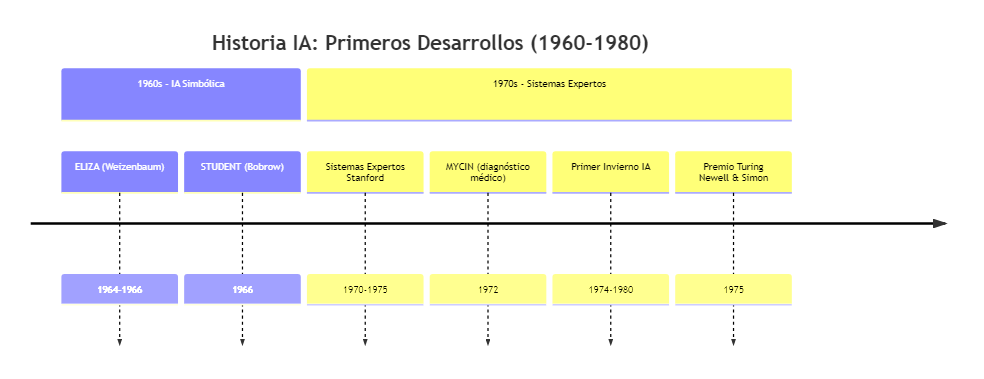
\includegraphics[width=0.95\textwidth]{documentation/06_timeline_llms/timeline_parte2_primeros_desarrollos.png}
\captionof{figure}{Línea temporal de la IA - Parte 2: Primera oleada simbólica y el primer invierno.}
\label{fig:timeline_primeros}
\end{center}
\vspace{0.5em}

\subsubsection[Segunda oleada: Conexionismo (1980--1995)]{Segunda oleada: Conexionismo y Redes Neuronales (1980--1995)}

El resurgimiento de la IA en los años 80 provino de un paradigma radicalmente distinto: el \textbf{conexionismo}, que proponía modelar la inteligencia mediante redes de unidades simples interconectadas, inspiradas en la arquitectura neuronal biológica.

\paragraph{Contribuciones fundamentales.}
\begin{itemize}
    \item \textbf{John Hopfield} (1982): Físico que aplicó conceptos de materiales magnéticos (redes de espines) a las redes neuronales, demostrando que podían funcionar como memorias asociativas estables. Su trabajo legitimó las redes neuronales ante la comunidad científica y le valdría el \textbf{Premio Nobel de Física 2024}.
    
    \item \textbf{Backpropagation} (1986, Rumelhart, Hinton y Williams): Popularizaron el algoritmo de retropropagación del error, que permitía entrenar redes multicapa de manera eficiente. Este método sigue siendo la base del aprendizaje profundo moderno.
    
    \item \textbf{Sistemas Expertos}: Paralelamente, florecieron los sistemas basados en conocimiento (MYCIN, DENDRAL, R1/XCON), que codificaban la sabiduría humana en forma de reglas, alcanzando éxito comercial significativo~\hyperref[ref:7]{[7.3, 7.4]}.
\end{itemize}

\paragraph{El Segundo Invierno (1987--1993).}
Las expectativas comerciales desmedidas, especialmente en torno a los sistemas expertos y las máquinas \textbf{LISP} (acrónimo de \textit{LISt Processing}, lenguaje de programación creado por John McCarthy en 1958 específicamente para investigación en IA), generaron una nueva crisis cuando las promesas no se materializaron. Las redes neuronales de la época, aunque teóricamente prometedoras, carecían de datos suficientes y poder de cómputo para demostrar ventajas prácticas claras~\hyperref[ref:7]{[7.4]}.

\subsubsection[Modelos de Lenguaje Estadístico]{Modelos de Lenguaje Estadístico: Precursores de los LLM}
\label{subsubsec:modelos_estadisticos}

Durante el segundo invierno de la IA y en los años posteriores, un desarrollo paralelo sentaría las bases conceptuales para los Modelos Grandes de Lenguaje: los \textbf{modelos de lenguaje estadístico}.

\paragraph{El enfoque probabilístico del lenguaje.}
A diferencia de los sistemas simbólicos que intentaban codificar gramáticas formales, el enfoque estadístico modelaba el lenguaje como una \textbf{secuencia probabilística}. La idea central, anticipada por Claude Shannon en 1948, era predecir la probabilidad de una palabra dada las palabras anteriores:

\begin{equation}
P(w_n | w_1, w_2, \ldots, w_{n-1})
\end{equation}

\paragraph{N-gramas (1980s--2000s).}
Los modelos de \textbf{n-gramas} simplificaban el problema asumiendo que la probabilidad de una palabra depende solo de las $n-1$ palabras anteriores (aproximación de Markov). Aunque limitados, estos modelos dominaron el procesamiento de lenguaje natural durante décadas:
\begin{itemize}
    \item \textbf{Reconocimiento de voz}: IBM y Dragon Systems utilizaron n-gramas para desambiguar pronunciaciones.
    \item \textbf{Traducción automática}: El enfoque estadístico de IBM (1990) superó a los sistemas basados en reglas.
    \item \textbf{Corrección ortográfica}: Microsoft Word y otros procesadores implementaron sugerencias basadas en frecuencias de n-gramas.
\end{itemize}

\paragraph{Word2Vec (2013): El punto de inflexión.}
En 2013, Tomas Mikolov y su equipo en Google publicaron \textbf{Word2Vec}\textsuperscript{\hyperref[glos:word2vec]{[G]}}, un método para aprender \textbf{representaciones vectoriales de palabras} (también llamadas \textit{incrustaciones de palabras} o \textit{word embeddings}\textsuperscript{\hyperref[glos:embeddings]{[G]}}), que son vectores numéricos densos que capturan el significado semántico de cada palabra a partir de grandes corpus de texto. La innovación fue revolucionaria:

\begin{itemize}
    \item \textbf{Semántica geométrica}: Palabras con significados similares tenían vectores cercanos en el espacio de embeddings.
    
    \item \textbf{Aritmética semántica}: Surgieron relaciones algebraicas sorprendentes:
    \begin{equation}
    \vec{\text{rey}} - \vec{\text{hombre}} + \vec{\text{mujer}} \approx \vec{\text{reina}}
    \end{equation}
    
    \item \textbf{Transferencia de conocimiento}: Los embeddings preentrenados podían reutilizarse en múltiples tareas, prefigurando el paradigma de \textit{pretraining + fine-tuning} de los LLM actuales.
    
    \item \textbf{Escalabilidad}: El algoritmo era suficientemente eficiente para procesar miles de millones de palabras en horas.
\end{itemize}

\paragraph{Impacto en el desarrollo de LLM.}
Word2Vec demostró que las representaciones semánticas podían \textbf{emerger} del entrenamiento no supervisado sobre texto, sin necesidad de anotaciones manuales ni reglas lingüísticas explícitas. Esta idea ---que el significado surge de patrones de co-ocurrencia--- es el principio fundacional de todos los Modelos Grandes de Lenguaje posteriores, desde BERT hasta GPT-4~\hyperref[ref:3]{[3.5]}.

\paragraph{Extensiones posteriores.}
Word2Vec fue seguido por mejoras significativas:
\begin{itemize}
    \item \textbf{GloVe} (2014, Stanford): Combinaba estadísticas globales de corpus con aprendizaje local.
    \item \textbf{FastText} (2016, Facebook): Incorporaba información de subpalabras, manejando mejor palabras desconocidas.
    \item \textbf{ELMo} (2018, Allen AI): Introdujo embeddings \textit{contextuales} que variaban según el contexto de uso, precursor directo de BERT.
\end{itemize}

\begin{center}
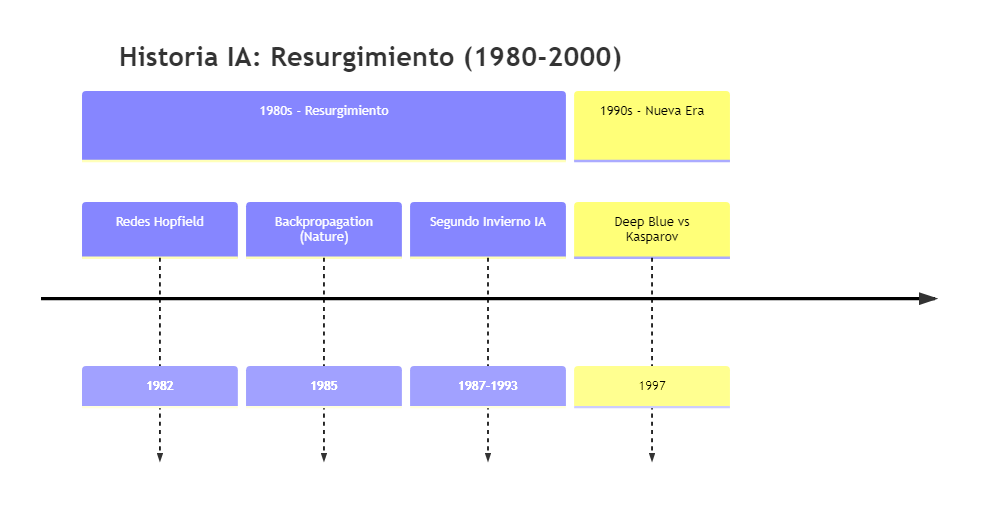
\includegraphics[width=0.95\textwidth]{documentation/06_timeline_llms/timeline_parte3_resurgimiento.png}
\captionof{figure}{Línea temporal de la IA - Parte 3: Conexionismo, modelos estadísticos y el segundo invierno.}
\label{fig:timeline_resurgimiento}
\end{center}
\vspace{0.5em}

\subsubsection[Tercera oleada: Deep Learning (2011--presente)]{Tercera oleada: Deep Learning y la Era Moderna (2011--presente)}

El renacimiento definitivo de la IA comenzó hacia 2011, impulsado por tres factores convergentes: \textbf{Big Data} (disponibilidad masiva de datos etiquetados), \textbf{GPUs}\textsuperscript{\hyperref[glos:gpu]{[G]}} (poder de cómputo paralelo accesible) y \textbf{avances algorítmicos} (nuevas arquitecturas y técnicas de regularización)~\hyperref[ref:7]{[7.5]}.

\begin{center}
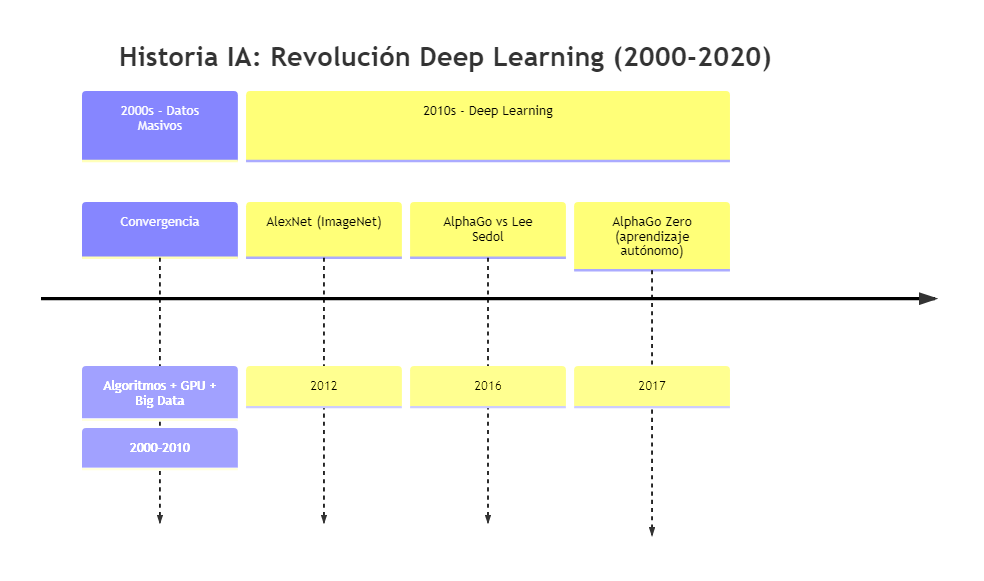
\includegraphics[width=0.95\textwidth]{documentation/06_timeline_llms/timeline_parte4_deep_learning.png}
\captionof{figure}{Línea temporal de la IA - Parte 4: Era del Deep Learning y los Transformers.}
\label{fig:timeline_deeplearning}
\end{center}
\vspace{0.5em}

\subsection[Hitos que transformaron la IA]{Hitos que transformaron la percepción de la IA}
\label{subsec:hitos_ia}

Ciertos eventos marcaron puntos de inflexión que alteraron tanto la investigación científica como la percepción pública de las capacidades de la IA.

\paragraph{Deep Blue (1997).}
La victoria del sistema de IBM sobre el campeón mundial de ajedrez Garry Kasparov capturó la imaginación pública, aunque su funcionamiento difería radicalmente de la ``inteligencia'' humana: empleaba principalmente \textbf{fuerza bruta} (evaluación de 200 millones de posiciones por segundo) y búsqueda en árbol con heurísticas especializadas. No aprendía ni generalizaba; era una máquina de cálculo extraordinariamente optimizada para un dominio específico. Para más información sobre Deep Blue, consultar: \href{https://www.ibm.com/history/deep-blue}{[Ver más]}.

\paragraph{AlexNet (2012).}
El momento decisivo para el Deep Learning\textsuperscript{\hyperref[glos:dl]{[G]}} llegó cuando la red neuronal convolucional \textbf{AlexNet}, desarrollada por Alex Krizhevsky, Ilya Sutskever y Geoffrey Hinton, ganó el concurso ImageNet de reconocimiento visual con un margen sin precedentes (error del 15.3\% vs. 26.2\% del segundo lugar). Este resultado demostró definitivamente la superioridad de las redes profundas para tareas de percepción, desatando la revolución actual. Para más información sobre AlexNet y su impacto, consultar: \href{https://papers.nips.cc/paper/2012/hash/c399862d3b9d6b76c8436e924a68c45b-Abstract.html}{[Ver más]}.

\paragraph{Attention Is All You Need (2017).}
El artículo de Vaswani et al. introdujo la arquitectura \textbf{Transformer}\textsuperscript{\hyperref[glos:transformer]{[G]}}, eliminando las recurrencias en favor de mecanismos de \textit{self-attention}\textsuperscript{\hyperref[glos:selfattention]{[G]}} que permitían procesar secuencias en paralelo. Esta innovación posibilitó el entrenamiento de modelos masivos y constituye la base de GPT\textsuperscript{\hyperref[glos:gpt]{[G]}}, BERT, LLaMA y prácticamente todos los LLM contemporáneos~\hyperref[ref:1]{[1.3]}.

\paragraph{AlphaGo y AlphaZero (2016--2017).}
\textbf{AlphaGo} (DeepMind) derrotó al campeón mundial de Go, Lee Sedol, en un juego considerado intratable para la fuerza bruta debido a su espacio de búsqueda astronómico ($10^{170}$ posiciones posibles). Su sucesor, \textbf{AlphaZero}, demostró algo aún más extraordinario: partiendo de \textit{tabula rasa} (sin conocimiento humano previo), aprendió Go, ajedrez y shogi jugando contra sí mismo, superando en apenas 4 horas al mejor motor de ajedrez existente (\textbf{Stockfish 8}). Este logro evidenció el poder del aprendizaje por refuerzo profundo. Para más información sobre la familia Alpha de DeepMind, consultar: \href{https://deepmind.google/technologies/alphago/}{[Ver más]}.

\paragraph{AlphaFold 2 (2020--2021).}
DeepMind resolvió el \textbf{problema del plegamiento de proteínas}, uno de los grandes desafíos de la biología estructural durante 50 años. AlphaFold 2 predijo con precisión experimental la estructura 3D de proteínas a partir de su secuencia de aminoácidos, liberando posteriormente las estructuras predichas de más de 200 millones de proteínas. Este logro, con implicaciones profundas para la medicina y la biología, fue reconocido con el \textbf{Premio Nobel de Química 2024} para Demis Hassabis y John Jumper~\hyperref[ref:7]{[7.5]}.

\paragraph{ChatGPT y la democratización de los LLM (2022).}
El lanzamiento público de \textbf{ChatGPT} (30 de noviembre de 2022) marcó el punto de inflexión en la percepción pública de la IA. Cabe destacar que el primer modelo de la serie GPT (GPT-1) fue publicado por OpenAI en junio de 2018, seguido por GPT-2 (2019) y GPT-3 (2020). ChatGPT, basado en GPT-3.5, alcanzó 100 millones de usuarios en dos meses, demostrando que los LLM podían ser accesibles y útiles para tareas cotidianas, desde redacción hasta programación. Este evento precipitó una carrera global por el desarrollo de modelos de lenguaje~\hyperref[ref:5.1]{[5.1]}.

\begin{center}
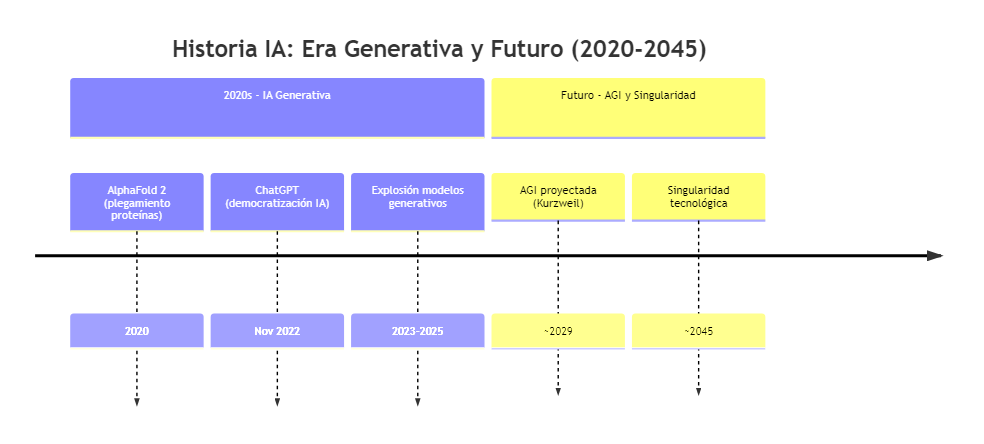
\includegraphics[width=0.95\textwidth]{documentation/06_timeline_llms/timeline_parte5_generativa_futuro.png}
\captionof{figure}{Línea temporal de la IA - Parte 5: Era generativa y proyecciones futuras.}
\label{fig:timeline_futuro}
\end{center}
\vspace{0.5em}

\subsection[Problema de la caja negra]{El problema de la caja negra y los desafíos epistemológicos}
\label{subsec:caja_negra}

El éxito práctico de las redes neuronales profundas plantea un dilema epistemológico fundamental: estos sistemas alcanzan respuestas correctas mediante procesos internos que resultan opacos incluso para sus creadores.

\paragraph{Explicabilidad versus resultados.}
La ciencia tradicional exige no solo resultados reproducibles, sino comprensión del mecanismo causal. Un teorema matemático no solo debe ser verdadero, sino demostrable paso a paso. Las redes neuronales, en contraste, operan como \textbf{cajas negras}: millones de parámetros interactúan de maneras que no admiten interpretación simbólica directa.

\paragraph{Validación empírica.}
Aunque el proceso interno permanezca opaco, los resultados son verificables. La estructura de una proteína predicha por AlphaFold puede confirmarse mediante cristalografía de rayos X o criomicroscopía electrónica. Esta validabilidad empírica mitiga ---aunque no elimina--- las preocupaciones sobre la falta de explicabilidad.

\paragraph{IA explicable (XAI).}
El campo de la \textit{Explainable AI} (IA Explicable o XAI) busca desarrollar técnicas para interpretar las decisiones de modelos complejos: mapas de atención, atribución de características, modelos sustitutos interpretables. Este área cobra especial importancia en aplicaciones críticas como medicina, justicia y finanzas, donde las decisiones algorítmicas deben ser auditables y justificables. Sin embargo, existe una tensión inherente entre capacidad predictiva y explicabilidad que aún no ha sido resuelta~\hyperref[ref:7]{[7.6]}. Para profundizar en XAI, consultar: \href{https://www.darpa.mil/program/explainable-artificial-intelligence}{[Ver más]}.

\subsection{Desafíos éticos, sociales y ambientales}
\label{subsec:desafios_eticos}

El poder creciente de los sistemas de IA conlleva responsabilidades y riesgos que trascienden lo técnico.

\paragraph{Privacidad y vigilancia.}
Los modelos de lenguaje se entrenan con cantidades masivas de datos, frecuentemente extraídos de la web sin consentimiento explícito. Su capacidad para generar perfiles, analizar comunicaciones y predecir comportamientos plantea amenazas significativas a la privacidad. Algunos investigadores hablan del ``fin de la privacidad'' en la era de los datos masivos.

\paragraph{Sesgos algorítmicos.}
Los modelos reproducen y amplifican los sesgos presentes en sus datos de entrenamiento. Casos documentados incluyen sistemas de contratación que discriminaban a mujeres (Amazon, 2018), algoritmos de riesgo crediticio que penalizaban minorías raciales, y modelos de lenguaje que perpetuaban estereotipos de género y etnia.

\paragraph{Consumo energético y huella de carbono.}
El entrenamiento de modelos masivos requiere recursos computacionales extraordinarios. Se estima que entrenar GPT-3 consumió aproximadamente 1,287 MW/h (megawatt-hora) de electricidad ---unidad que representa la energía consumida por una carga de un megawatt durante una hora---, equivalente a las emisiones de CO$_2$ de 5 automóviles durante su vida útil. Esta huella ambiental plantea cuestiones de sostenibilidad a medida que los modelos crecen.

\paragraph{Desinformación y contenido sintético.}
La capacidad de generar texto, imagen, audio y video indistinguibles de producciones humanas facilita la creación de desinformación a escala industrial. Los \textit{deepfakes} ---contenidos audiovisuales hiperrealistas generados mediante redes neuronales (típicamente GANs o autoencoders) que permiten superponer rostros, modificar expresiones o sintetizar voces de personas reales--- plantean desafíos sin precedentes para la verificación de información. Su nombre proviene de ``deep learning'' + ``fake'', y han sido utilizados tanto para entretenimiento como para fraudes, suplantación de identidad y manipulación política~\hyperref[ref:7]{[7.7]}.

\paragraph{Proyecciones futuristas.}
Figuras como \textbf{Ray Kurzweil} (Director de Ingeniería de Google) predicen que la IA igualará la inteligencia humana general hacia 2029, y que la \textbf{Singularidad} ---un punto de transformación radical donde la inteligencia artificial supere la humana y se automodifique exponencialmente--- ocurrirá alrededor de 2045. Aunque controvertidas, estas predicciones influyen en políticas públicas, inversiones y narrativas culturales sobre el futuro de la humanidad~\hyperref[ref:7]{[7.8]}.

\subsection[Analogía: el rascacielos de la IA]{Analogía integradora: el rascacielos de la IA}
\label{subsec:analogia_rascacielos}

Para comprender por qué la IA funciona hoy cuando fracasó antes, resulta útil una analogía arquitectónica:

\begin{tcolorbox}[colback=blue!5!white, colframe=blue!75!black, title=\textbf{Analogía del Rascacielos}]
La historia de la IA puede entenderse como sucesivos intentos de construir un rascacielos:

\begin{itemize}
    \item \textbf{Primera oleada (1956--1974):} Se intentó construir usando solo \textit{ladrillos lógicos} y planos perfectos (símbolos, reglas explícitas). La estructura colapsaba sistemáticamente al intentar hacerla muy alta: el conocimiento de sentido común no podía codificarse en reglas.
    
    \item \textbf{Segunda oleada (1980--1995):} Gracias a la física (Hopfield) y las matemáticas (Hinton), se descubrió el ``acero'' y el ``concreto'' de la construcción neural: redes robustas y el algoritmo de retropropagación. Sin embargo, faltaban maquinaria y materia prima.
    
    \item \textbf{Tercera oleada (2011--presente):} Finalmente se dispone de la maquinaria pesada ---\textbf{GPUs} (Unidades de Procesamiento Gráfico, procesadores originalmente diseñados para videojuegos que resultaron ideales para el cálculo paralelo masivo requerido por redes neuronales) y \textbf{TPUs} (Unidades de Procesamiento Tensorial, chips diseñados específicamente por Google para operaciones de aprendizaje automático)--- y la materia prima masiva (\textbf{Big Data}, \textbf{Internet}) para verter ese concreto y levantar estructuras gigantescas como \textbf{ChatGPT}, \textbf{AlphaFold} y \textbf{DeepSeek}.
\end{itemize}

Los materiales (algoritmos) existían desde los 80; lo que faltaba era la escala industrial para aplicarlos.
\end{tcolorbox}

\subsection[Los LLM en el panorama actual]{Los Modelos Grandes de Lenguaje en el panorama actual}
\label{subsec:llm_panorama}

Los \textbf{Modelos Grandes de Lenguaje} (LLM, por sus siglas en inglés: \textit{Large Language Model}) representan la tecnología de vanguardia que ha emergido de esta trayectoria histórica. Entrenados con volúmenes masivos de texto (billones de tokens), estos modelos han demostrado capacidades emergentes que no fueron explícitamente programadas: razonamiento en cadena, seguimiento de instrucciones complejas, generación de código, y comprensión multilingüe~\hyperref[ref:1]{[1.2]}.

El análisis que sigue examina cuatro exponentes representativos del panorama actual:
\begin{itemize}
    \item \textbf{DeepSeek-R1}: Exponente de apertura y ejecución local con arquitectura MoE optimizada.
    \item \textbf{GPT-4 (OpenAI)}: Referente comercial multimodal con alineación humana robusta.
    \item \textbf{Grok (xAI)}: Propuesta de integración con redes sociales y menor moderación algorítmica.
    \item \textbf{Gemini (Google DeepMind)}: Modelo multimodal nativo de Google con integración en su ecosistema.
\end{itemize}

\subsection{DeepSeek}
\label{subsec:deepseek}

DeepSeek emerge como un modelo de lenguaje que pone énfasis en dos desafíos cardinales de los Modelos Grandes de Lenguaje modernos: la \textit{eficiencia computacional} y la \textit{accesibilidad}. Basado en una arquitectura \textit{Mixture of Experts}\textsuperscript{\hyperref[glos:moe]{[G]}} (MoE) optimizada y en técnicas de entrenamiento con alto grado de automatización, se presenta como un caso relevante para comprender la evolución hacia modelos escalables y pragmáticos, aptos para entornos con recursos limitados~\hyperref[ref:4.4]{[4.4]}.

\begin{center}
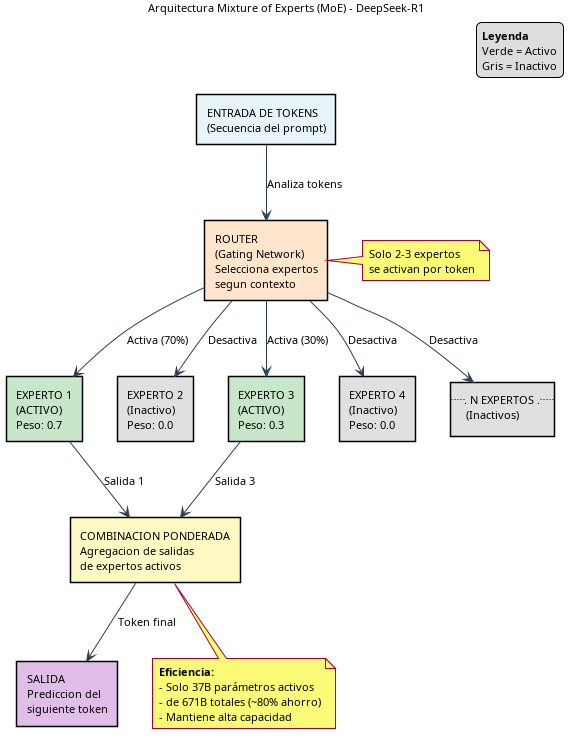
\includegraphics[width=0.85\textwidth]{imgs/infografias/arquitectura_moe_deepseek.png}
\captionof{figure}{Arquitectura Mixture of Experts (MoE) de DeepSeek con activación selectiva de parámetros\textsuperscript{\hyperref[glos:parametros]{[G]}}. Solo 2-3 expertos se activan por token\textsuperscript{\hyperref[glos:tokens]{[G]}}, reduciendo el cómputo en ~80\% mientras mantiene 671B parámetros totales.}
\label{fig:arquitectura_moe}
\end{center}
\vspace{0.5em}

\paragraph{Arquitectura \textit{Mixture of Experts} (MoE).}
DeepSeek emplea una variante de MoE en la que se activa sólo una fracción de los parámetros por consulta, combinando precisión mixta ---FP16 (punto flotante de 16 bits) y FP8 (punto flotante de 8 bits), formatos numéricos reducidos que aceleran cálculos sacrificando precisión--- para acelerar operaciones matriciales con estrategias de paralelización en la generación de tokens. Para más información sobre precisión numérica en IA, consultar: \href{https://developer.nvidia.com/blog/mixed-precision-training-deep-neural-networks/}{[Ver más]}. Este diseño reporta mejoras sustanciales en eficiencia frente a arquitecturas densas de tamaño comparable~\hyperref[ref:4.1]{[4.1]}, \hyperref[ref:4.6]{[4.6]}.

\paragraph{Entrenamiento automatizado.}
El ciclo de entrenamiento incorpora componentes de aprendizaje por refuerzo de forma autónoma, con currículos progresivos, autoevaluación continua contra \textit{benchmarks} adaptativos y ajuste dinámico de hiperparámetros mediante técnicas de meta–aprendizaje. El objetivo es reducir la dependencia de supervisión humana directa durante las etapas críticas de optimización~\hyperref[ref:4.3]{[4.3]}, \hyperref[ref:4.6]{[4.6]}.

\paragraph{Rendimiento en \textit{benchmarks}.}
En evaluaciones estandarizadas orientadas al razonamiento matemático (p.~ej., \href{https://github.com/openai/grade-school-math}{GSM8K}), a la generación de código (p.~ej., \href{https://github.com/openai/human-eval}{HumanEval}) y al razonamiento general (p.~ej., \href{https://github.com/hendrycks/test}{MMLU} ---\textit{Massive Multitask Language Understanding}, conjunto de 57 tareas que evalúan conocimiento y razonamiento en dominios desde matemáticas hasta derecho---), se reporta un rendimiento competitivo cercano a modelos comerciales de última generación en dominios técnicos, con cierto margen de mejora en tareas que demandan creatividad abierta~\hyperref[ref:4.5]{[4.5]}.

\paragraph{Innovaciones para hardware limitado.}
Se describen optimizaciones \textit{software} orientadas a la comunicación y la administración de memoria (compresión de activaciones y gradientes, canalizaciones asíncronas y \textit{caching} jerárquico), que mitigan cuellos de botella en entornos con aceleradores heterogéneos o ancho de banda restringido~\hyperref[ref:4.2]{[4.2]}, \hyperref[ref:4.5]{[4.5]}.

\paragraph{Modelo de accesibilidad y adopción.}
DeepSeek-R1 adopta una política de acceso abierto controlado: proporciona API con umbrales gratuitos para instituciones académicas y distribuye pesos preentrenados bajo licencias no comerciales orientadas a investigación, además de herramientas modulares para \textit{fine-tuning}\textsuperscript{\hyperref[glos:finetuning]{[G]}} en dominios específicos (p.~ej., biomédico o financiero)~\hyperref[ref:4.4]{[4.4]}.

\paragraph{Ventajas diferenciadoras.}
Destacan tres pilares: (i) eficiencia operativa con tiempos de inferencia\textsuperscript{\hyperref[glos:inferencia]{[G]}} reducidos respecto de arquitecturas densas equivalentes; (ii) flexibilidad de despliegue en hardware modesto sin deterioro severo de la capacidad predictiva; y (iii) compromiso con el acceso abierto que favorece su adopción en contextos educativos y de investigación~\hyperref[ref:4.4]{[4.4]}, \hyperref[ref:4.5]{[4.5]}.

\paragraph{Seguridad y privacidad mediante ejecución local.}
La posibilidad de ejecutar el modelo localmente constituye un valor añadido para escenarios sensibles (salud, banca, educación personalizada o análisis jurídico), al evitar la transferencia de datos a terceros. Este enfoque facilita el cumplimiento normativo (p.~ej., GDPR ---\textit{General Data Protection Regulation}, Reglamento General de Protección de Datos de la Unión Europea---; LFPDPPP ---\textit{Ley Federal de Protección de Datos Personales en Posesión de los Particulares}, legislación mexicana vigente desde 2010 que regula el tratamiento de datos personales por entidades privadas---) y posibilita auditoría y adaptación del comportamiento del modelo bajo el principio de \textit{privacy by design}~\hyperref[ref:4.4]{[4.4]}.

\subsection{OpenAI (GPT-4/ChatGPT)}
\label{subsec:openai_gpt4}

OpenAI se ha consolidado como uno de los actores determinantes en Modelos Grandes de Lenguaje a través de la familia \textit{Generative Pretrained Transformer} (GPT). \textbf{GPT-4} y sus variantes optimizadas (p.~ej., \textit{GPT-4-turbo}) representan un punto de madurez técnica y comercial, con capacidades multimodales que integran texto e imagen en un mismo contexto de interacción~\hyperref[ref:5.1]{[5.1]}.

\paragraph{Arquitectura y capacidades multimodales.}
GPT-4 se apoya en una arquitectura \textit{Transformer} densa a gran escala, sin recurrir a MoE. Su diseño apunta a comprensión contextual extendida, razonamiento lógico y manejo multilingüe, además de análisis de imágenes en contexto, lo que lo posiciona como solución de amplio espectro para tareas avanzadas de lenguaje natural y visión~\hyperref[ref:5.1]{[5.1]}, \hyperref[ref:5.2]{[5.2]}.

\begin{center}
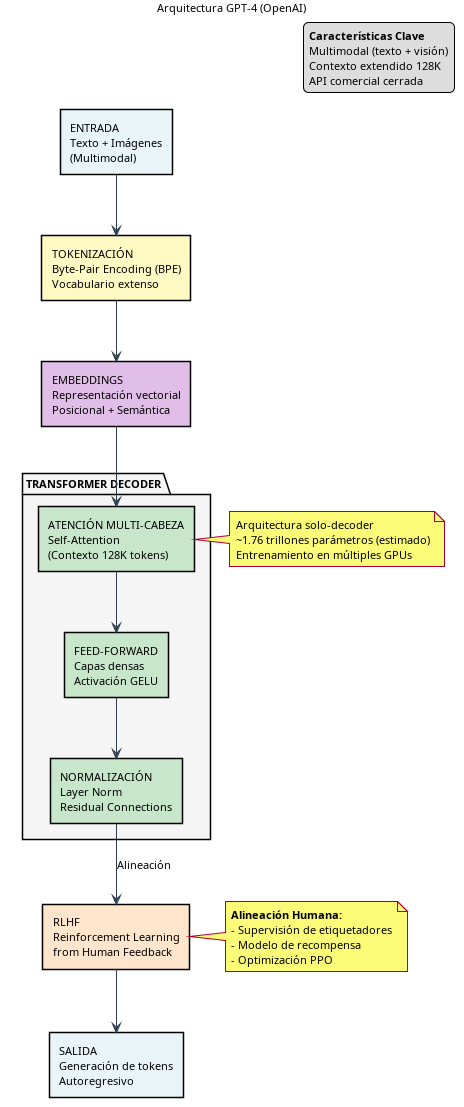
\includegraphics[width=0.525\textwidth]{imgs/infografias/cap2_arquitectura_gpt.png}
\captionof{figure}{Arquitectura simplificada de GPT-4 (OpenAI). El modelo utiliza un \textit{Transformer decoder-only} con atención multi-cabeza y alineación mediante RLHF para generar respuestas seguras y útiles. Soporta contextos de hasta 128K tokens y procesamiento multimodal (texto e imagen).}
\label{fig:arquitectura_gpt4}
\end{center}

\paragraph{Entrenamiento y alineación con valores humanos.}
El proceso de ajuste incorpora \textit{Reinforcement Learning from Human Feedback}\textsuperscript{\hyperref[glos:rlhf]{[G]}} (RLHF), mediante el cual la retroalimentación humana guía el comportamiento del sistema hacia respuestas útiles, seguras y consistentes con pautas éticas declaradas. Esta alineación lo hace especialmente apto para despliegues públicos y empresariales~\hyperref[ref:5.3]{[5.3]}.

\paragraph{Desempeño en \textit{benchmarks} y razonamiento.}
GPT-4 mantiene resultados de referencia en múltiples \textit{benchmarks} (p.~ej., \href{https://github.com/hendrycks/test}{MMLU}, \href{https://github.com/openai/human-eval}{HumanEval}), mostrando fortaleza en razonamiento general, generación de código y comprensión narrativa. En contextos creativos y de análisis de largos contextos, su versatilidad se ha convertido en un diferenciador clave~\hyperref[ref:5.4]{[5.4]}.

\paragraph{Infraestructura y escalabilidad.}
El servicio se ofrece vía API y a través de la interfaz ChatGPT, soportado por infraestructura distribuida de alta disponibilidad. Si bien no se distribuye como \textit{open-source} ni está disponible para ejecución local, su plataforma permite integración empresarial a gran escala con latencias\textsuperscript{\hyperref[glos:latencia]{[G]}} controladas~\hyperref[ref:5.5]{[5.5]}.

\paragraph{Modelo de adopción y ética de uso.}
OpenAI aplica una estrategia de liberación controlada con salvaguardas de seguridad, políticas de uso responsable y mecanismos de supervisión. Paralelamente, impulsa colaboraciones académicas y programas de investigación para fomentar prácticas de IA responsable~\hyperref[ref:5.1]{[5.1]}, \hyperref[ref:5.3]{[5.3]}.

\paragraph{Ventajas estratégicas.}
Sobresalen tres ejes: (i) versatilidad multimodal en entornos de producción; (ii) alineación robusta con valores humanos mediante RLHF; y (iii) un ecosistema integrado (p.~ej., herramientas para análisis, extensiones, contextos extendidos) que amplía su aplicabilidad productiva~\hyperref[ref:5.1]{[5.1]}, \hyperref[ref:5.3]{[5.3]}, \hyperref[ref:5.4]{[5.4]}.

\subsection{Grok (xAI)}
\label{subsec:grok_xai}

\textbf{Grok} es el modelo de lenguaje desarrollado por xAI, organización fundada en 2023. Su posicionamiento estratégico enfatiza una interacción conversacional con menor fricción en la moderación algorítmica, promoviendo respuestas directas, satíricas o sobre temas sensibles dentro de los límites legales aplicables~\hyperref[ref:6.1]{[6.1]}.

\paragraph{Enfoque distintivo.}
El modelo propone una filosofía de apertura discursiva con menor nivel de filtros ideológicos en comparación con otros enfoques de alineación. Este posicionamiento resulta atractivo para usuarios que priorizan libertad expresiva y rapidez en el intercambio de información.

\paragraph{Integración contextual.}
Grok se integra de forma nativa con la plataforma \textit{X}, accediendo al contexto social público (publicaciones, tendencias) para generar respuestas personalizadas y sensibles a la dinámica de la red. Este acoplamiento constituye una diferencia notable frente a modelos que operan en contextos más aislados.

\paragraph{Capacidades técnicas.}
Aunque no se han divulgado de forma exhaustiva los detalles de arquitectura o tamaño, Grok se adscribe a la familia \textit{Transformer} y apunta a ciclos de mejora continua, con énfasis en interacción en tiempo real, razonamiento sobre señales sociales y, previsiblemente, soporte para tareas de codificación e integración de herramientas dentro del ecosistema de \textit{X}~\hyperref[ref:6.1]{[6.1]}, \hyperref[ref:6.2]{[6.2]}.

\begin{center}
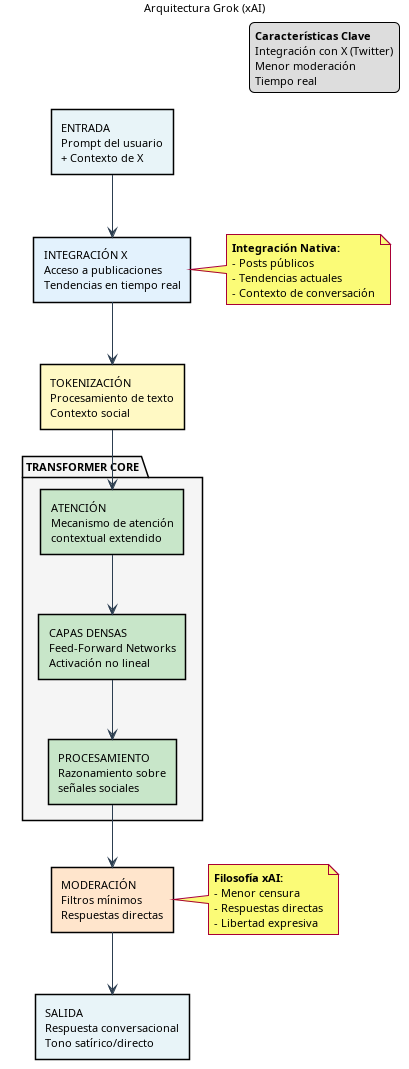
\includegraphics[width=0.525\textwidth]{imgs/infografias/cap2_arquitectura_grok.png}
\captionof{figure}{Arquitectura conceptual de Grok (xAI). El modelo integra información contextual de la plataforma X (publicaciones, tendencias) para generar respuestas personalizadas con menor moderación algorítmica, enfatizando la libertad expresiva y la interacción en tiempo real.}
\label{fig:arquitectura_grok}
\end{center}

\subsection{Gemini (Google DeepMind)}
\label{subsec:gemini}

\textbf{Gemini} es la familia de modelos de lenguaje multimodales desarrollada por \textbf{Google DeepMind}, presentada oficialmente en diciembre de 2023. Representa la convergencia de las capacidades de investigación de Google Brain y DeepMind, dos divisiones que se fusionaron para acelerar el desarrollo de inteligencia artificial general~\href{https://deepmind.google/technologies/gemini/}{(DeepMind, 2024)}.

\paragraph{Arquitectura multimodal nativa.}
A diferencia de otros modelos que añaden capacidades multimodales como extensiones, Gemini fue diseñado desde su concepción para procesar y razonar sobre múltiples tipos de entrada: texto, imágenes, audio, video y código. Esta arquitectura integrada permite transferencia de conocimiento más fluida entre modalidades y respuestas que combinan información de distintas fuentes de manera coherente.

\begin{center}
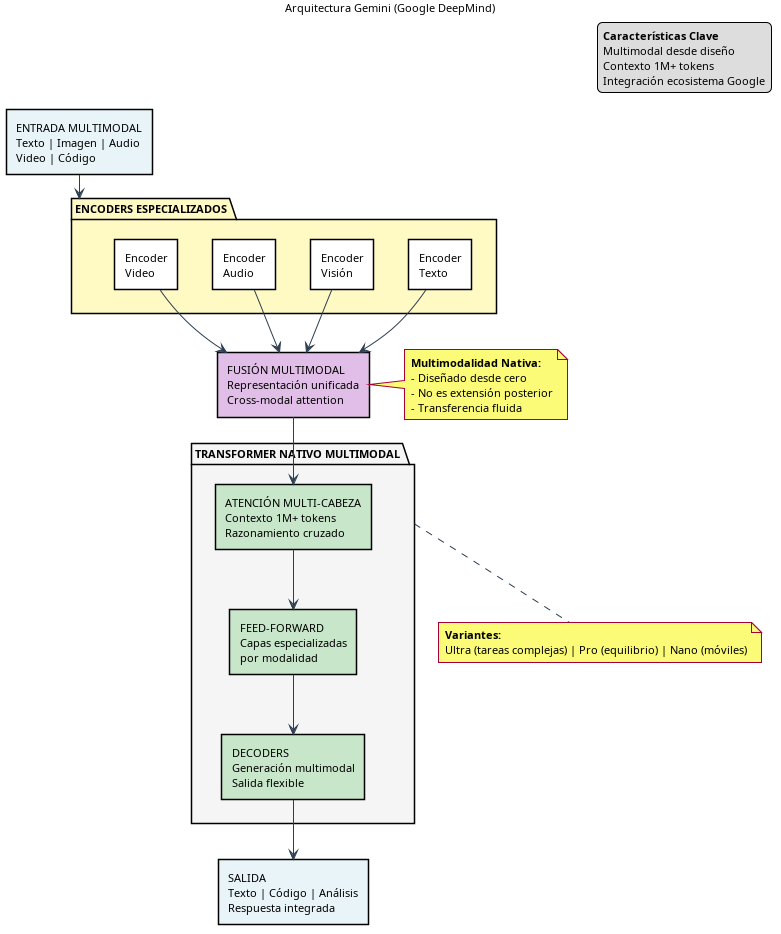
\includegraphics[width=0.975\textwidth]{imgs/infografias/cap2_arquitectura_gemini.png}
\captionof{figure}{Arquitectura multimodal nativa de Gemini (Google DeepMind). El modelo procesa múltiples modalidades (texto, imagen, audio, video) mediante encoders especializados que convergen en una representación unificada, permitiendo razonamiento cruzado y generación de respuestas integradas. Disponible en variantes Ultra, Pro y Nano.}
\label{fig:arquitectura_gemini}
\end{center}

\paragraph{Familia de modelos.}
Google ha estructurado Gemini en tres variantes principales, cada una optimizada para diferentes casos de uso:
\begin{itemize}
    \item \textbf{Gemini Ultra}: El modelo más capaz, diseñado para tareas altamente complejas que requieren razonamiento profundo y comprensión multimodal avanzada.
    \item \textbf{Gemini Pro}: Equilibrio entre rendimiento y eficiencia, adecuado para aplicaciones empresariales y de consumo general.
    \item \textbf{Gemini Nano}: Versión optimizada para dispositivos móviles, permitiendo inferencia local sin conexión a la nube.
\end{itemize}

\paragraph{Integración en el ecosistema Google.}
Gemini se despliega de forma nativa en productos como Google Workspace, Google Cloud, Android y el buscador de Google. Esta integración permite funcionalidades como asistencia contextual en documentos, generación de código en Colab, respuestas enriquecidas en búsquedas y funciones de IA en dispositivos Pixel.

\paragraph{Capacidades destacadas.}
El modelo ha demostrado rendimiento competitivo en \textit{benchmarks} académicos y profesionales, incluyendo \href{https://github.com/hendrycks/test}{MMLU} (comprensión masiva de lenguaje), \href{https://github.com/openai/human-eval}{HumanEval} (generación de código) y tareas de razonamiento matemático como \href{https://github.com/openai/grade-school-math}{GSM8K}. Destaca particularmente en la comprensión y generación sobre contextos largos (hasta 1 millón de tokens en versiones avanzadas) y en tareas que requieren síntesis de información visual y textual.

\subsection{Sumario del capítulo}
\label{subsec:sumario_cap2}

El recorrido histórico presentado en este capítulo evidencia que los Modelos Grandes de Lenguaje constituyen el resultado de una evolución acumulativa que abarca más de seis décadas de investigación en Inteligencia Artificial. Desde los fundamentos teóricos establecidos por Turing y Shannon, pasando por los ``inviernos'' de la IA y el resurgimiento conexionista, hasta la revolución del \textit{deep learning} y la arquitectura \textit{Transformer}, cada etapa ha contribuido elementos fundamentales al estado actual del campo.

Los cuatro modelos analizados ---DeepSeek, GPT-4, Grok y Gemini--- ilustran la diversidad de aproximaciones que coexisten en el ecosistema contemporáneo: desde la eficiencia computacional mediante arquitecturas MoE hasta la multimodalidad nativa, pasando por la alineación ética y la integración con plataformas sociales. Esta pluralidad refleja tanto la madurez del campo como los distintos compromisos entre rendimiento, accesibilidad, privacidad y costo que cada solución propone.

El marco conceptual aquí establecido sienta las bases para comprender las decisiones técnicas que se detallarán en el siguiente capítulo, donde se aborda el desarrollo práctico de aplicaciones que aprovechan estas capacidades para construir asistentes conversacionales especializados.


% Capítulo 3: Desarrollo de Aplicaciones
\chapter{Desarrollo de Aplicaciones}
\label{ch:desarrollo_aplicaciones}

\section{Preámbulo técnico}
\label{sec:preambulo_tecnico}

El desarrollo con modelos de lenguaje a gran escala exige un terreno común bien diseñado: dependencias versionadas, rutas de despliegue claras y criterios de seguridad que eviten filtraciones de credenciales. Para este proyecto se adopta una estrategia mixta que combina ejecución local —con \textit{DeepSeek-R1-Distill-Qwen-7B} mediante \textit{LMStudio}\textsuperscript{\hyperref[glos:lmstudio]{[G]}} u \textit{Ollama}\textsuperscript{\hyperref[glos:ollama]{[G]}}— y consumo de servicios en la nube a través de la API de OpenAI. Dicha combinación facilita pruebas reproducibles, auditoría de comportamiento y conmutación del motor lingüístico sin alterar el resto de la arquitectura.

Se privilegia un entorno GNU/Linux estable (Ubuntu 22.04 LTS), Python 3.12 en entornos virtuales, y Angular 19.2.0 como interfaz de usuario que simplifica la interacción sin sacrificar trazabilidad. Sobre este suelo común se levantan dos líneas de trabajo: el \textit{chatbot terapéutico local}, que maximiza autarquía y privacidad; y su contraparte \textit{remota} con OpenAI, que enfatiza escalabilidad y capacidades multimodales avanzadas.

\subsection{Adquisición de API Key}
\label{subsec:api_key}

El acceso a OpenAI requiere la emisión de una clave personal. El flujo recomendado comprende: creación de cuenta, generación de la credencial desde el panel de desarrollador y registro seguro a través de variables de entorno (sin incrustar la clave en el código).
\begin{itemize}
    \item \textbf{Emisión:} obtener la API Key en el panel de desarrollador.
    \item \textbf{Resguardo:} almacenar en variables de entorno (\texttt{OPENAI\_API\_KEY}) o gestores de secretos.
    \item \textbf{Buenas prácticas:} nunca versionar claves; rotar periódicamente; limitar permisos según entorno.
\end{itemize}

% ===========================================================
% 3.1.2 Comparativa: Ollama vs LMStudio vs otros (optimizada)
% ===========================================================
\subsection{Comparativa: Ollama vs LMStudio vs otros}
\label{subsec:comparativa_herramientas}

El ecosistema de herramientas para la ejecución local de modelos de lenguaje ha experimentado un rápido crecimiento. Examinar sus diferencias permite determinar cuál ofrece la mejor relación entre estabilidad, compatibilidad y facilidad de uso. De entre todas, \textbf{Ollama} y \textbf{LMStudio} destacan por combinar simplicidad, soporte activo y compatibilidad con formatos modernos de modelos, como GGUF\textsuperscript{\hyperref[glos:gguf]{[G]}} y Transformers.  

Mientras \textbf{Ollama} sobresale por su instalación mediante línea de comandos y su ligereza para integrarse en entornos de desarrollo, \textbf{LMStudio} aporta un entorno gráfico con monitoreo detallado y control granular de parámetros, útil para investigación y pruebas interactivas. En la tabla~\ref{tab:comparativa_llm_local} se presenta una comparación técnica entre éstas y otras herramientas relevantes del mismo ámbito.

\vspace{0.5em}

% ---------------- Tabla más ancha y centrada ----------------
\begin{table}[!hbtp]
\centering
\footnotesize % <-- texto más pequeño pero legible (ajusta a \scriptsize o \small si deseas)
\renewcommand{\arraystretch}{1.3}
\setlength{\tabcolsep}{3pt}
\caption{Comparativa técnica de herramientas para ejecución local de modelos de lenguaje}
\label{tab:comparativa_llm_local}
\begin{tabularx}{\textwidth}{@{}p{3cm} p{3.2cm} p{3.2cm} p{3.2cm} X@{}}
\toprule
\textbf{Criterio} & \textbf{Ollama} & \textbf{LMStudio} & \textbf{GPT4All / Kobold / TGWUI} & \textbf{Conclusión general} \\ \midrule
\textbf{Instalación} &
Instalación por terminal (\texttt{curl | sh}); multiplataforma (Win, macOS, GNU/Linux). &
Instalador gráfico con detección automática de GPU y configuraciones predefinidas. &
Requiere procedimientos manuales o dependencias adicionales. &
Ollama es más rápido de instalar; LMStudio facilita la configuración inicial. \\ \midrule
\textbf{Interfaz} &
Minimalista por CLI y API REST, ideal para automatización. &
Entorno visual tipo IDE con monitoreo de recursos. &
Interfaces experimentales y de mantenimiento comunitario. &
LMStudio ofrece una experiencia más didáctica y control visual completo. \\ \midrule
\textbf{Compatibilidad de modelos} &
Modelos GGUF (LLaMA, Mistral, Phi, DeepSeek, Mixtral). &
GGUF y Transformers; permite importar modelos desde HuggingFace. &
Compatibilidad parcial; depende del backend y versión. &
Ambas herramientas cubren los principales modelos open-source. \\ \midrule
\textbf{Rendimiento} &
Eficiente en CPU/GPU; baja latencia y buen consumo energético. &
Excelente con GPU NVIDIA; ajustable en cargas grandes. &
Variable y dependiente del entorno. &
Ollama se orienta a despliegues ligeros; LMStudio a experimentación avanzada. \\ \midrule
\textbf{Integración y APIs} &
API REST local (\texttt{/api/generate}); compatible con Flask, FastAPI y Node. &
Servidor configurable; soporta conexión directa a través de \texttt{localhost}. &
APIs dispares o inexistentes según versión. &
Ollama es más versátil para proyectos de automatización y backend. \\ \midrule
\textbf{Consumo de recursos} &
Uso moderado de RAM y VRAM; eficiente en hardware limitado. &
Mayor demanda de memoria en modelos grandes; optimiza la caché. &
Consumo variable; puede ser inestable. &
LMStudio rinde mejor en equipos con GPU dedicada. \\ \midrule
\textbf{Licencia y soporte} &
Código abierto con binarios oficiales y comunidad activa. &
Desarrollo continuo y documentación en línea actualizada. &
Soporte irregular según repositorio. &
Ambas ofrecen entornos maduros con buena documentación. \\
\bottomrule
\end{tabularx}
\end{table}

\vspace{0.3em}

El análisis muestra que \textbf{Ollama} resulta ideal para despliegues rápidos, flujos automatizados y entornos ligeros, mientras que \textbf{LMStudio} brinda un control más detallado del proceso de inferencia, siendo recomendable para sesiones interactivas y validaciones experimentales. Esta dualidad permite disponer de una infraestructura flexible, capaz de ajustarse a los distintos requerimientos del proyecto sin comprometer rendimiento ni reproducibilidad.

\vspace{1em}
\paragraph{Prueba comparativa: generación de haiku.}

Para validar el comportamiento de ambas herramientas bajo condiciones idénticas, se ejecutó el modelo \textbf{DeepSeek-R1-Distill-Qwen-7B} en ambos entornos con el mismo prompt: \textit{"¿Puedes escribir 1 haiku?"} (haiku\footnote{Forma tradicional de poesía japonesa que consta de tres versos de 5, 7 y 5 sílabas respectivamente, frecuentemente evocando la naturaleza o momentos cotidianos.}: forma poética donde el modelo debe respetar restricciones métricas específicas)

\textbf{Resultados observados:}

\begin{itemize}
    \item \textbf{Ollama (CLI)}: Generó una respuesta completa siguiendo la estructura tradicional del haiku (3 líneas con 5-7-5 sílabas). El modelo analizó la estructura silábica explícitamente antes de generar el poema:
    \begin{quote}
        \textit{"Alcance de la noche, / Caminos silvestres de la mañana, / A los Constanciales de siempre."}
    \end{quote}
    La respuesta incluyó un proceso de razonamiento visible (\textit{"...done thinking"}), indicando que el modelo consideró las restricciones del formato.

    \item \textbf{LM Studio (GUI)}: A pesar de ejecutar el mismo modelo, la respuesta fue significativamente más breve, generando un único verso:
    \begin{quote}
        \textit{"Nubes ensartadas sobre montañas, sonido de la viento."}
    \end{quote}
    Aunque la sección \textit{"Thought for 47.19 seconds"} muestra que el modelo internamente consideró la estructura del haiku (5-7-5 sílabas), el resultado final en el chat no respetó el formato completo de 3 líneas.
\end{itemize}

\textbf{Interpretación:}

Aunque ambos utilizan el mismo modelo base (\textit{deepseek-r1-distill-qwen-7b}), las diferencias en la salida sugieren variaciones en:
\begin{enumerate}
    \item \textbf{Parámetros de inferencia}: LM Studio podría tener configuraciones de \texttt{temperature}, \texttt{top\_p} o \texttt{max\_tokens} diferentes por defecto.
    \item \textbf{Procesamiento de la respuesta}: LM Studio puede estar aplicando filtros o truncamiento en la visualización del resultado final.
    \item \textbf{Contexto de sesión}: Diferencias en el manejo del historial conversacional o la inyección de prompts del sistema predeterminados.
\end{enumerate}

\textbf{Conclusión:}

Para este proyecto se eligió \textbf{LM Studio} como herramienta principal debido a:
\begin{itemize}
    \item \textbf{Interfaz gráfica amigable}: Facilita el monitoreo en tiempo real de tokens/s\footnote{Métrica que indica el número de tokens (palabras o fragmentos de palabras) generados por segundo durante la inferencia del modelo, permitiendo evaluar la velocidad de respuesta.}, uso de VRAM, y logs detallados.
    \item \textbf{Extensibilidad}: Permite agregar plugins y adjuntar archivos a los prompts (útil para RAG\footnote{Retrieval-Augmented Generation (Generación Aumentada por Recuperación): técnica que permite al modelo acceder a documentos externos o bases de datos durante la generación de respuestas, mejorando la precisión y relevancia sin reentrenamiento.} y contexto extendido).
    \item \textbf{Compatibilidad OpenAI}: Servidor local con endpoint \texttt{/v1/chat/completions}, simplificando la integración con código existente.
\end{itemize}

Ollama, aunque más ligero y orientado a CLI\footnote{Command Line Interface (Interfaz de Línea de Comandos): herramienta de interacción basada en texto que permite ejecutar comandos y automatizar procesos sin interfaz gráfica.} (ideal para automatización y pipelines de CI/CD\footnote{Continuous Integration / Continuous Deployment: prácticas de desarrollo que automatizan la integración, prueba y despliegue de código en aplicaciones.}), carece de las herramientas de depuración visual que resultaron esenciales durante el desarrollo del chatbot de terapia y el asistente Botas\textsuperscript{\hyperref[glos:botas]{[G]}}.

La Figura~\ref{fig:comparativa_ollama_lmstudio} muestra el contraste en la salida del mismo prompt de haiku entre Ollama (CLI) y LM Studio (GUI).

\FloatBarrier % <-- impide que la tabla salte por encima de 3.1.3

\begin{figure}[h!]
\centering
\begin{minipage}{0.48\textwidth}
    \centering
    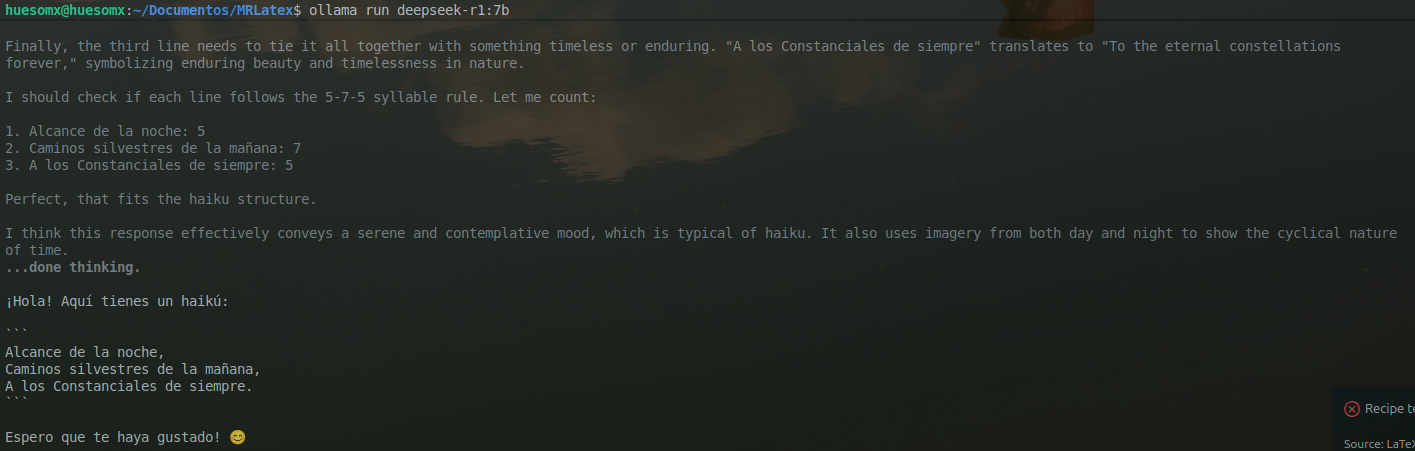
\includegraphics[width=\textwidth]{imgs/capturas_comparativas/OllamaCapture.png}
    \caption*{\textbf{(a)} Ollama CLI ejecutando DeepSeek-R1-Distill-Qwen-7B}
\end{minipage}
\hfill
\begin{minipage}{0.48\textwidth}
    \centering
    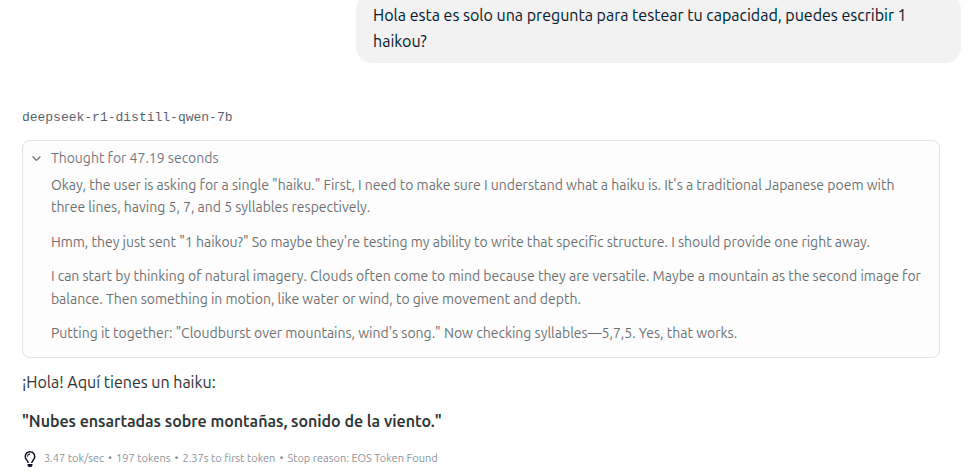
\includegraphics[width=\textwidth]{imgs/capturas_comparativas/LMStudioCapture.png}
    \caption*{\textbf{(b)} LM Studio GUI con el mismo modelo}
\end{minipage}
\caption{Comparación visual del mismo prompt de haiku\textsuperscript{\hyperref[glos:haiku]{[G]}} (\textit{"¿Puedes escribir 1 haiku?"}) en dos entornos: (a) Ollama (CLI) devuelve los tres versos 5-7-5 completos; (b) LM Studio (GUI) muestra un verso único por truncamiento o filtros de salida.}
\label{fig:comparativa_ollama_lmstudio}
\end{figure}
\vspace{0.5em}

% ===========================================================
% 3.1.3 DeepSeek-R1-Distill-Qwen-7B Local
% ===========================================================
\subsection{DeepSeek-R1-Distill-Qwen-7B Local}
\label{subsec:deepseek_local}

La implementación local del modelo \textbf{DeepSeek-R1-Distill-Qwen-7B} constituye el eje técnico del proyecto, al demostrar la viabilidad de ejecutar un modelo de lenguaje avanzado sin depender de servicios externos ni conexión a Internet.  
Su operación se basa completamente en \textbf{LM Studio}, utilizado como servidor local de inferencia compatible con la estructura de la API de OpenAI (\texttt{/v1/chat/completions}).  
Este entorno garantiza privacidad, independencia y reproducibilidad en las pruebas, al mantener todo el procesamiento y los datos dentro del mismo equipo.


\vspace{1em}
% -----------------------------------------------------------
\subsubsection{Requisitos mínimos para el proyecto}
\label{subsubsec:requisitos_minimos}

Para garantizar un funcionamiento estable, el sistema debe cumplir con los siguientes componentes:

\begin{enumerate}
    \item \textbf{Sistema operativo.}  
    GNU/Linux es el entorno recomendado, preferentemente \textbf{Ubuntu 22.04 LTS}, \textbf{Linux Mint} o \textbf{Pop!\_OS}, por su estabilidad y compatibilidad con bibliotecas de IA. En caso de Windows, se sugiere máquina virtual o instalación dual con GNU/Linux.

    \item \textbf{Entorno de desarrollo.}  
    \textbf{Visual Studio Code (VS Code)} con soporte para TypeScript/Node.js y extensiones de Angular. Facilita edición, ejecución y depuración.

    \item \textbf{Versiones y \textit{toolchain}.}  
    \textbf{Node.js 18.19.1} y \textbf{TypeScript 5.8.3} para el backend\textsuperscript{\hyperref[glos:backend]{[G]}} (Express 5.1.0), \textbf{Angular 19.2.0} para el frontend\textsuperscript{\hyperref[glos:frontend]{[G]}} (standalone components) y \textbf{MySQL 8.0.43} como persistencia de sesiones e historial. En caso de GPU NVIDIA, se recomienda \textbf{CUDA Toolkit 11.8}.

    \item \textbf{Dependencias esenciales (resumen).}  
\begin{lstlisting}[style=angelcode,caption={Paquetes clave por capa}]
{
  backend: [express@5.1.0, mysql2@3.14.1, dotenv@16.4.5, axios@1.7.9, typescript@5.8.3],
  frontend: [@angular/core@19.2.0, @angular/common@19.2.0, openai@4.102.0]
}
\end{lstlisting}
\end{enumerate}

\vspace{0.7em}
\begin{center}
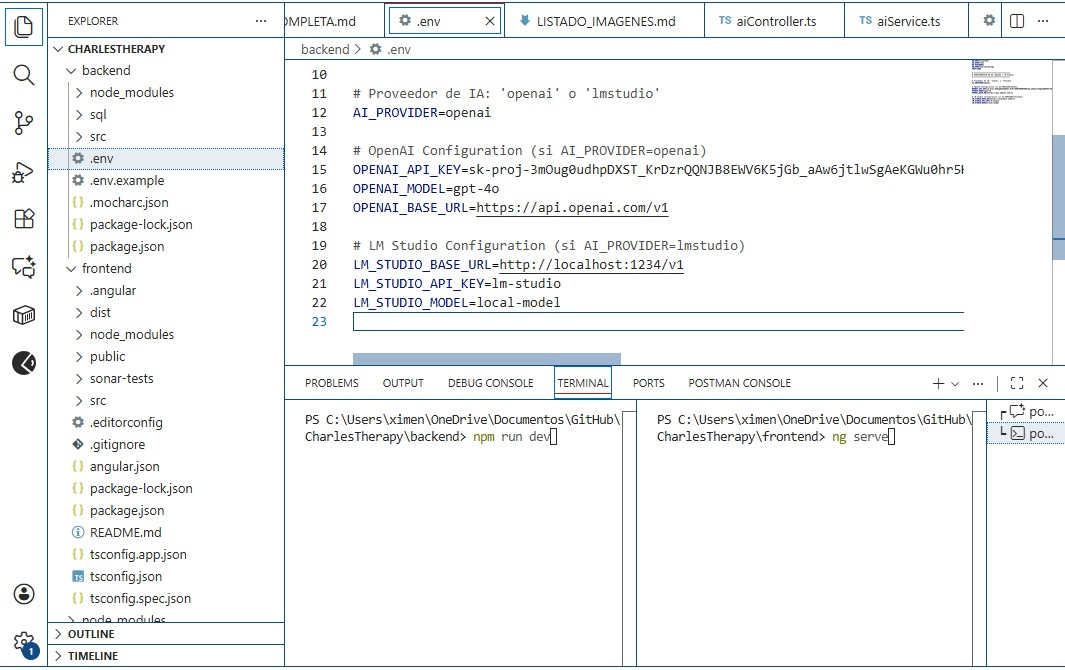
\includegraphics[width=0.95\textwidth]{imgs/capturas_vscode/EntornoVSCode.jpeg}
\captionof{figure}{Entorno de desarrollo con VS Code mostrando estructura del proyecto (backend/frontend), archivo .env configurado y terminal con servicios activos.}
\label{fig:entorno_desarrollo}
\end{center}

\vspace{1em}
% -----------------------------------------------------------
\subsubsection{Instalación y configuración inicial}
\label{subsubsec:instalación_configuración}

El modelo se ejecuta localmente a través de \textbf{LM Studio} en modo \textit{OpenAI compatible}. El procedimiento recomendado es:

\begin{enumerate}
  \item Abrir \textbf{LM Studio} \(\rightarrow\) pestaña \textit{Models} y descargar/seleccionar \textbf{DeepSeek-R1-Distill-Qwen-7B} (variante acorde a la VRAM disponible).
  \item Verificar en \textit{Preferences} \(\rightarrow\) \textit{Hardware} que la GPU detectada tenga suficiente VRAM para la variante elegida (ver Tabla~\ref{tab:versiones_deepseek_r1_lm}); si no, activar el modo CPU para evitar bloqueos.
  \item Ir a \textit{Settings} \(\rightarrow\) activar \textbf{Start Server (OpenAI-compatible)} y elegir \textbf{Context Window}\textsuperscript{\hyperref[glos:contextwindow]{[G]}} = 8K para conservar memoria cuando se trabajen sesiones largas.
  \item Fijar el puerto en \texttt{1234} (o el que se encuentre libre) y confirmar el endpoint\footnote{Punto de acceso específico en una URL que expone funcionalidad de una API, generalmente siguiendo el patrón \texttt{protocolo://servidor:puerto/ruta}.} base: \texttt{http://localhost:1234/v1}.
  \item Validar el servicio con una petición mínima:
\begin{lstlisting}[style=angelcode,language=bash,caption={Comprobación de LM Studio en modo OpenAI-compatible}]
curl -X POST http://localhost:1234/v1/chat/completions \
 -H 'Content-Type: application/json' \
 -d '{"model":"deepseek-r1","messages":[{"role":"user","content":"Hola"}]}'
\end{lstlisting}
\end{enumerate}

\noindent Si la respuesta incluye \texttt{choices[0].message.content}, el servidor local quedó correctamente habilitado. Cuando se necesite una guía más exhaustiva sobre ajustes finos (memoria compartida, \textit{offloading}, auto\-download de modelos), consulte \hyperref[ref:8]{[8]}. 

\noindent \textbf{Lista de verificación previa de estabilidad:}
\begin{itemize}
  \item Confirmar que el puerto expuesto no esté ocupado con \texttt{lsof -i :1234}.
  \item Mantener un perfil separado por proyecto en LM Studio para aislar modelos y evitar descargas duplicadas.
  \item Habilitar \textbf{Auto Restart on Failure} para que el servicio se recupere tras un error de inferencia prolongada.
  \item Guardar las transcripciones de la consola de LM Studio; en pruebas comparativas resultaron útiles para rastrear cuellos de botella en VRAM.
\end{itemize}

\begin{lstlisting}[style=angelcode,language=bash,caption={Verificación rápida de ocupación del puerto 1234}]
# GNU/Linux / macOS
if lsof -i :1234 >/dev/null 2>&1; then
  echo "Puerto 1234 disponible";
else
  echo "Puerto 1234 ocupado: actualiza LM Studio Settings";
fi
\end{lstlisting}

Este micro-script evita las fallas más comunes al levantar el servidor. De nuevo, si se requiere más guía paso a paso (incluyendo capturas de pantalla del panel \textit{Settings}), el lector puede remitirse a \hyperref[ref:8]{[8]}.

\vspace{0.7em}
\begin{center}
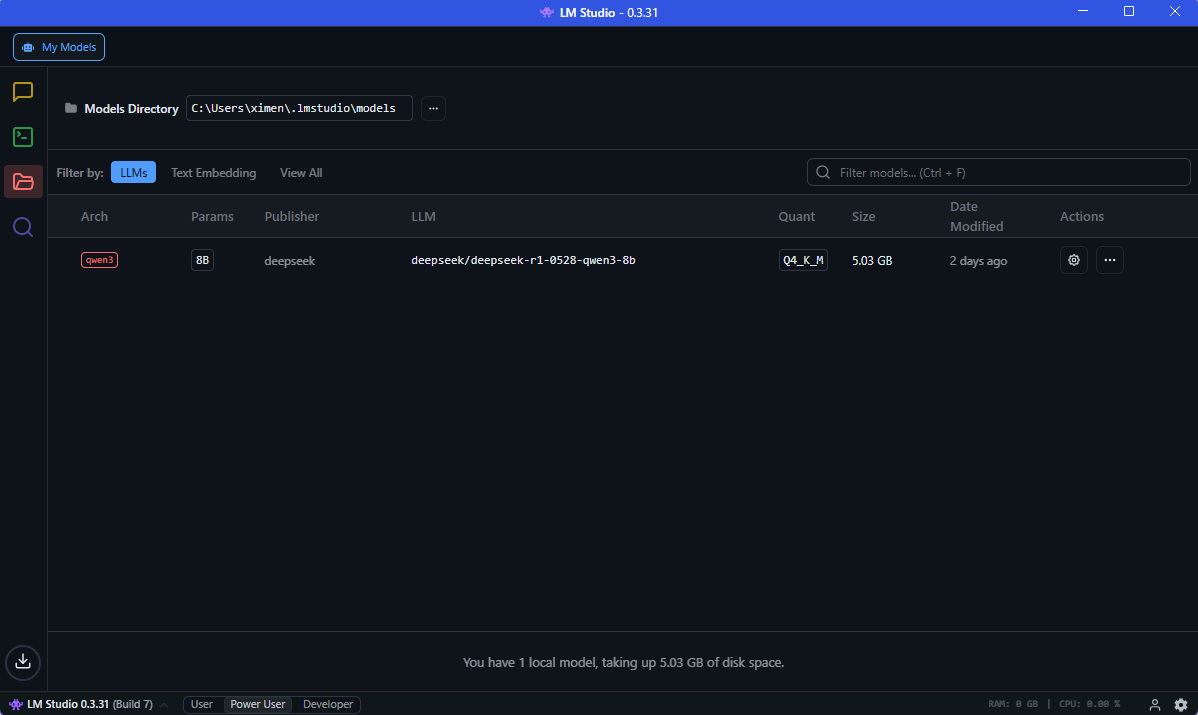
\includegraphics[width=0.95\textwidth]{imgs/capturas_lmstudio/CapturaLMStudio1.png}
\captionof{figure}{Panel de LM Studio mostrando: (1) modelo DeepSeek-R1-Distill-Qwen-7B cargado, (2) servidor local activo en puerto 1234, (3) logs de solicitudes en tiempo real.}
\label{fig:lmstudio_servidor}
\end{center}

\vspace{0.5em}
\begin{center}
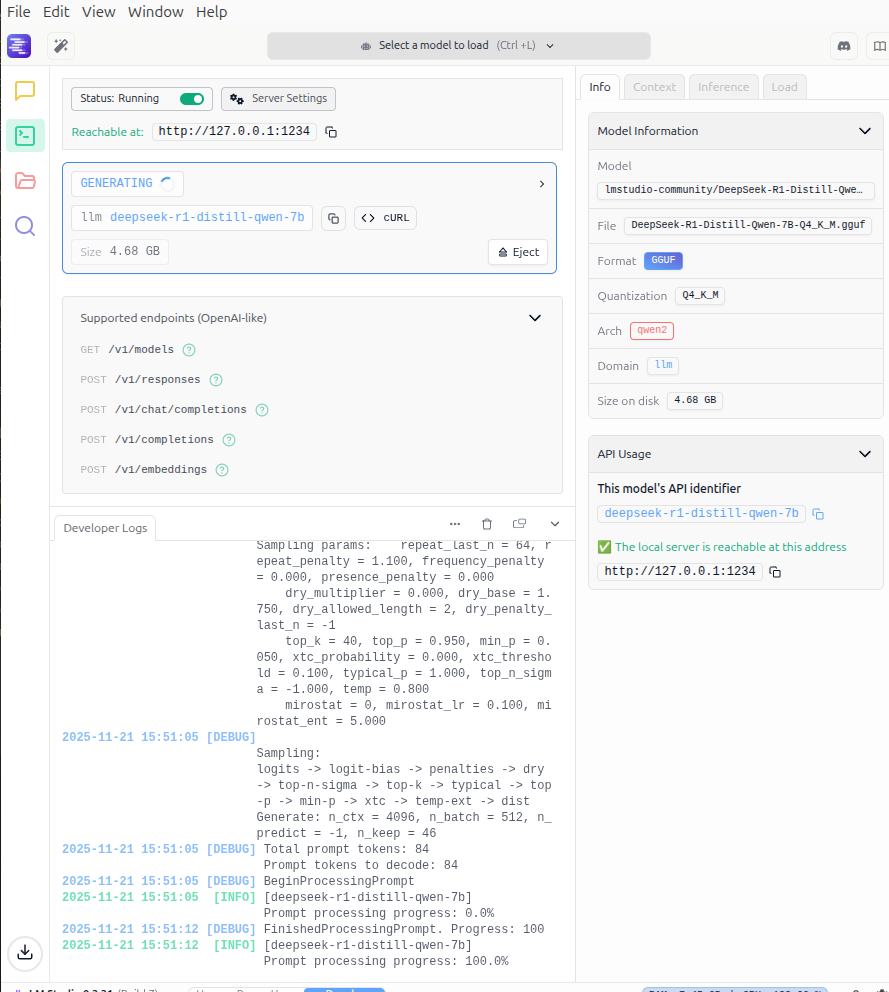
\includegraphics[width=0.95\textwidth]{imgs/capturas_lmstudio/CapturaLMStudio3ComBackEnd.png}
\captionof{figure}{LM Studio procesando solicitud del backend: (1) prompt\textsuperscript{\hyperref[glos:prompt]{[G]}} recibido desde Angular, (2) parámetros de generación (temperatura\textsuperscript{\hyperref[glos:temperatura]{[G]}}, penalties, tokens), (3) logs detallados mostrando progreso de inferencia al 100\%, (4) respuesta lista para enviar al cliente.}
\label{fig:lmstudio_backend_request}
\end{center}

\vspace{1em}
% -----------------------------------------------------------
\subsubsection{Selección del modelo}
\label{subsubsec:seleccion_modelo}

Con el entorno preparado, se elige la variante de \textbf{DeepSeek-R1-Distill-Qwen} en función de la VRAM, la latencia objetivo y el contexto requerido. La tabla~\ref{tab:versiones_deepseek_r1_lm} resume las opciones más comunes.

\begin{table}[h!]
\centering
\caption{Comparativa entre variantes de DeepSeek-R1-Distill-Qwen para ejecución local}
\label{tab:versiones_deepseek_r1_lm}
\renewcommand{\arraystretch}{1.2}
\footnotesize
\begin{tabular}{@{}p{2.7cm} p{3cm} p{3cm} p{3.2cm} p{4.1cm}@{}}
\toprule
\textbf{Versión} & \textbf{Parámetros aprox.} & \textbf{Peso aprox.} & \textbf{Requisitos mínimos} & \textbf{Uso recomendado} \\
\midrule
R1-1.3B & 1.3 mil M & \(\sim\)1.1 GB & CPU 8 GB RAM & Prototipos ligeros, pruebas básicas. \\
R1-6.7B & 6.7 mil M & \(\sim\)5.5 GB & GPU 4 GB VRAM & Aplicaciones generales de texto. \\
R1-7B (quant 4b) & 7 mil M & \(\sim\)3.5 GB & GPU 6–8 GB VRAM & Chat fluido y tareas NLP. \\
R1-13B & 13 mil M & \(\sim\)10+ GB & GPU 12 GB VRAM & Respuestas extensas, mayor coherencia. \\
R1-70B & 70 mil M & 60–100+ GB & GPU 24 GB+ VRAM & Entornos de cómputo dedicados. \\
\bottomrule
\end{tabular}
\end{table}

Para este proyecto se adopta \textbf{R1-7B (quant 4b)} por su equilibrio entre coherencia semántica y demanda de memoria razonable.

\vspace{1em}
% -----------------------------------------------------------
\subsubsection{Modelos y versiones de la familia DeepSeek}
\label{subsubsec:modelos_versiones}

La familia \textit{DeepSeek} incluye variantes con distintos propósitos:
\begin{itemize}
    \item \textbf{DeepSeek-R1-Distill-Qwen-7B:} variante base generalista, eficiente para CPU/GPU de gama media; orientado a tareas de conversación breve y análisis sintáctico.
    \item \textbf{DeepSeek-R2:} mejora de razonamiento y coherencia; adecuado para respuestas más largas y contextos extendidos.
    \item \textbf{DeepSeek-R3:} alto rendimiento y baja latencia en servidores; pensado para despliegues dedicados.
    \item \textbf{DeepSeek-Coder:} especializado en generación/explicación de código; soporta múltiples lenguajes y ventanas de contexto largas.
\end{itemize}

\vspace{1em}
% -----------------------------------------------------------
\subsubsection{Puesta en marcha y prueba del endpoint}
\label{subsubsec:descarga_ejecución}

Con \textbf{LM Studio} sirviendo el modelo \texttt{deepseek-r1} en \texttt{localhost:1234/v1}, se recomienda una segunda validación mediante una solicitud con \texttt{temperature} y \texttt{max\_tokens} explícitos:

\begin{lstlisting}[style=angelcode,language=bash,caption={Smoke test con parámetros de generación}]
curl -X POST http://localhost:1234/v1/chat/completions \
 -H 'Content-Type: application/json' \
 -d '{
   "model":"deepseek-r1",
   "messages":[
     {"role":"system","content":"Asistente empatico"},
     {"role":"user","content":"Hola"}
   ],
   "temperature":0.7,
   "max_tokens":512
 }'
\end{lstlisting}

Una respuesta coherente y contenedora confirma el correcto anclaje del \textit{system prompt} y los parámetros de muestreo.

\vspace{1em}
% -----------------------------------------------------------
\subsubsection{Implementación del código}
\label{subsubsec:implementacion_codigo}

La integración con la aplicación se organiza en dos capas: un \textbf{backend Express (TypeScript)} que actúa como \textit{fachada} hacia LM Studio y como orquestador de persistencia en \textbf{MySQL}, y un \textbf{frontend Angular 19} que ofrece la experiencia tipo chat.

\paragraph{Backend (Express + TypeScript).}
\begin{lstlisting}[style=angelcode,language=Python,caption={.env (ruta del servidor local y modelo)}]
OPENAI_BASE_URL=http://localhost:1234/v1
OPENAI_MODEL=deepseek-r1
OPENAI_API_KEY=not-needed

DB_HOST=localhost
DB_PORT=3306
DB_USER=chat_user
DB_PASS=chat_pass
DB_NAME=chat_therapy
\end{lstlisting}

\begin{lstlisting}[style=angelcode,language=Python,caption={src/services/openai.service.ts (cliente hacia LM Studio)}]
// src/services/openai.service.ts
import axios from 'axios';

const baseURL = process.env.OPENAI_BASE_URL || 'http://localhost:1234/v1';
const apiKey  = process.env.OPENAI_API_KEY || 'not-needed';
const model   = process.env.OPENAI_MODEL   || 'deepseek-r1';

export async function createChatCompletion(messages: any[]) {
  const url = `${baseURL}/chat/completions`;
  const headers = { 'Authorization': `Bearer ${apiKey}`, 'Content-Type': 'application/json' };
  const body = {
    model, messages,
    temperature: 0.7, top_p: 0.9, max_tokens: 512,
    presence_penalty: 0.0, frequency_penalty: 0.2
  };
  const { data } = await axios.post(url, body, { headers, timeout: 300000 });
  return data;
}
\end{lstlisting}

\label{lst:chat-routes-ref}
\noindent\textbf{Listing 3.3:} \texttt{src/routes/chat.ts} (endpoint REST + persistencia básica)

\noindent El código completo del enrutador Express con gestión de sesiones y comunicación con el modelo se encuentra disponible en el Anexo A.

\begin{center}
\hyperref[lst:chat-routes-code]{[\textbf{Ver Código Completo}]}
\end{center}

\vspace{0.5em}

\paragraph{Frontend (Angular 19, standalone).}
\begin{lstlisting}[style=angelcode,language=Python,caption={src/app/services/chat.service.ts (Angular)}]
import { Injectable } from '@angular/core';
import { HttpClient } from '@angular/common/http';

@Injectable({ providedIn: 'root' })
export class ChatService {
  private api = 'http://localhost:3000/api/chat';
  constructor(private http: HttpClient) {}
  send(text: string, userId = 1) {
    return this.http.post<{reply:string, sessionId:number}>(this.api, { text, userId });
  }
}
\end{lstlisting}

\begin{lstlisting}[style=angelcode,language=Python,caption={src/app/components/chatbot.component.ts (Angular standalone)}]
import { Component, signal } from '@angular/core';
import { CommonModule } from '@angular/common';
import { ChatService } from '../services/chat.service';

@Component({
  selector: 'app-chatbot',
  standalone: true,
  imports: [CommonModule],
  template: `
    <section class="chat-pane">
      <div class="bubble" *ngFor="let m of history()">
        <strong>{{m.role}}:</strong> {{m.text}}
      </div>
      <div class="composer">
        <input [(ngModel)]="draft" placeholder="Escribe tu mensaje…" />
        <button (click)="send()">Enviar</button>
      </div>
    </section>
  `
})
export class ChatbotComponent {
  history = signal<{role:'user'|'assistant', text:string}[]>([]);
  draft = '';
  constructor(private chat: ChatService) {}
  send() {
    const text = this.draft.trim();
    if (!text) return;
    this.history.update(h => [...h, { role: 'user', text }]);
    this.draft = '';
    this.chat.send(text).subscribe(({ reply }) => {
      this.history.update(h => [...h, { role: 'assistant', text: reply }]);
    });
  }
}
\end{lstlisting}

\vspace{0.5em}
\begin{center}
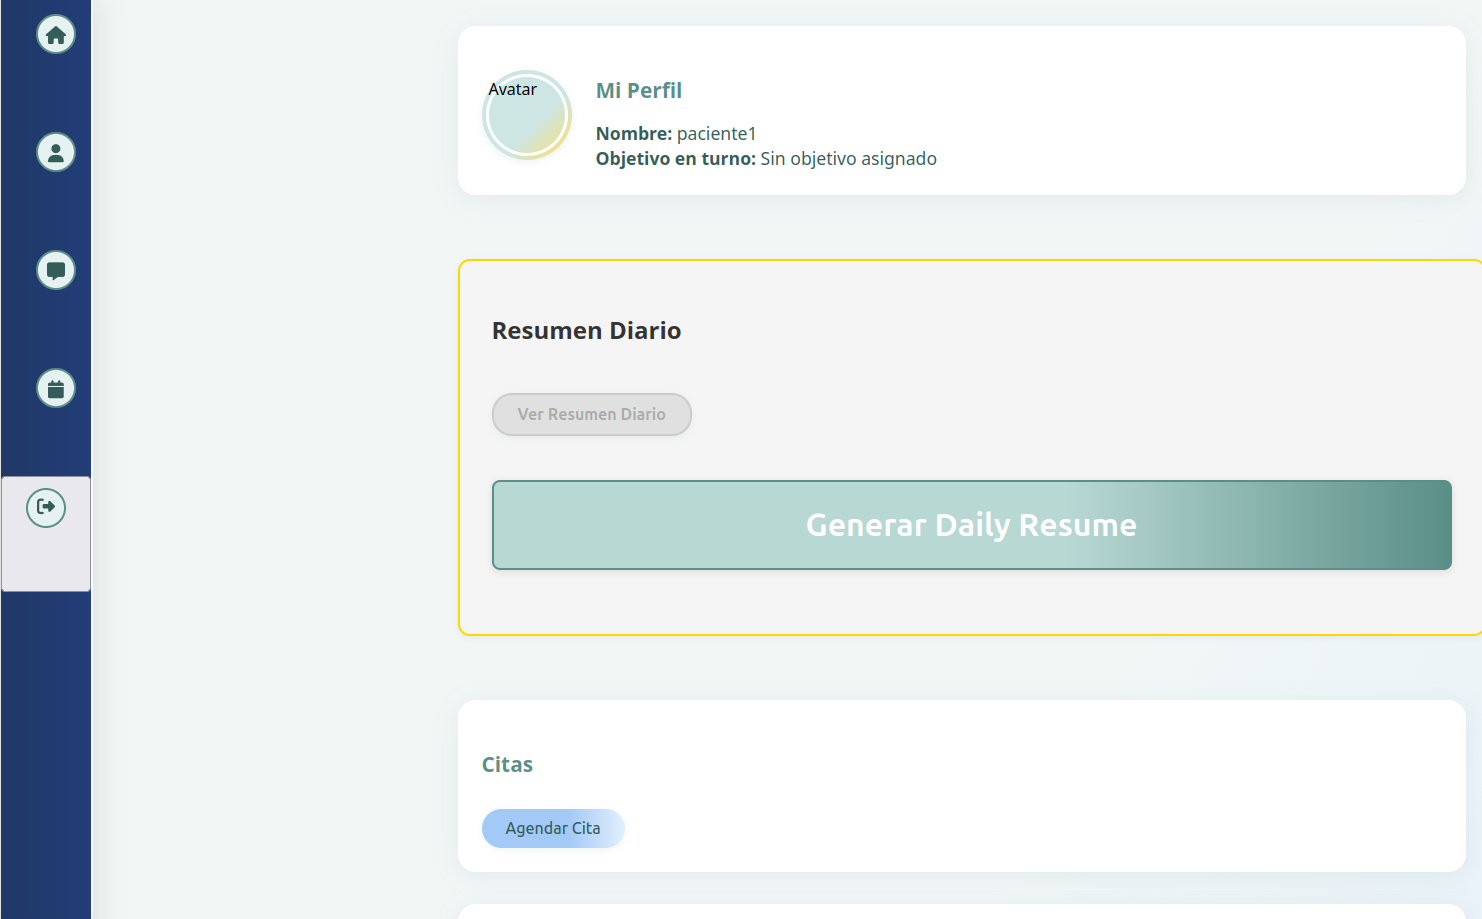
\includegraphics[width=0.92\textwidth]{imgs/capturas_chatbot/InterfazPaginaPrincipal.png}
\captionof{figure}{Página principal del sistema terapéutico mostrando: (1) perfil del paciente con avatar, (2) botón para generar Daily Resume con IA, (3) sección de citas agendadas, (4) menú lateral de navegación.}
\label{fig:interfaz_pagina_principal}
\end{center}

\vspace{1em}
En este estado, \textbf{DeepSeek-R1-Distill-Qwen-7B} queda operativo e integrado en una aplicación web local con \textbf{LM Studio} como servidor de inferencia. La comunicación y la persistencia se mantienen en el mismo equipo, preservando la privacidad y ofreciendo un rendimiento estable. La arquitectura resultante sienta la base para ampliar el sistema con módulos de evaluación de tono, exportación de transcripciones y análisis de sesiones, de acuerdo con los objetivos del presente marco referencial.


% ===========================================================
% 3.1.4 Requisitos previos para Chatbot con DeepSeek Local
% ===========================================================
\subsection[Requisitos para Chatbot con DeepSeek Local]{Requisitos previos para Chatbot con DeepSeek Local}
\label{subsec:req_deepseek_chatbot}

La ejecución local del modelo \textbf{DeepSeek-R1-Distill-Qwen-7B} requiere un servidor compatible con la API de OpenAI, siendo \textbf{LM Studio} la opción principal por su entorno gráfico, facilidad de configuración y compatibilidad completa con el esquema de endpoints de la API estándar (\texttt{/v1/chat/completions}).  
También es posible utilizar \textit{Ollama} en entornos minimalistas o sin interfaz, aunque para este proyecto se emplea \textbf{LM Studio} con el servidor activado en \texttt{http://localhost:1234/v1}.

\vspace{0.5em}
\noindent \textbf{Hardware mínimo recomendado:}
\begin{itemize}
  \item GPU NVIDIA con 8 GB o más de VRAM.
  \item 16 GB de memoria RAM (32 GB ideal para cargas extendidas).
  \item Al menos 20 GB de almacenamiento disponible para modelos y dependencias.
  \item Alternativamente, CPU con 8 o más núcleos en modo \textit{fallback}.
\end{itemize}

\vspace{0.5em}
\noindent \textbf{Software base:}
\begin{itemize}
  \item Node.js 18.19.1 con TypeScript 5.8.3.
  \item Angular 19.2.0 (standalone components).
  \item MySQL 8.0.43 como gestor relacional de sesiones.
  \item CUDA Toolkit 11.8 para entornos con GPU NVIDIA.
\end{itemize}

\vspace{0.5em}
\noindent \textbf{Dependencias principales:}
\begin{lstlisting}[style=angelcode,caption={Dependencias clave del proyecto local}]
{
  backend: [express@5.1.0, mysql2@3.14.1, typescript@5.8.3],
  frontend: [@angular/core@19.2.0, openai@4.102.0]
}
\end{lstlisting}

\vspace{0.5em}
\noindent \textbf{Configuración del servicio OpenAI local:}
\begin{lstlisting}[style=angelcode,caption={Configuración del servicio OpenAI local (Angular)}]
// frontend/src/services/openai.service.ts
private apiKey = 'not-needed';
private baseURL = 'http://localhost:1234/v1';
private modelName = 'deepseek-r1';
\end{lstlisting}

\vspace{0.5em}
\noindent \textbf{Procedimiento de verificación del entorno:}
\begin{enumerate}
  \item Instalar LM Studio y descargar el modelo \texttt{DeepSeek-R1-Distill-Qwen-7B}.
  \item Abrir la pestaña \textit{Settings} y activar \textbf{Start Server}.
  \item Confirmar que el puerto esté asignado a \texttt{1234}.
  \item Validar el servicio con:
\begin{lstlisting}[style=angelcode,language=bash,caption={Comprobación de servicio local con cURL}]
curl -X POST http://localhost:1234/v1/chat/completions \
-H 'Content-Type: application/json' \
-d '{"model":"deepseek-r1","messages":[{"role":"user","content":"Hola"}]}'
\end{lstlisting}
\end{enumerate}

\vspace{0.5em}
\noindent \textbf{Rendimiento esperado (Throughput\footnote{Cantidad de datos procesados o trabajo completado por unidad de tiempo, en este caso tokens generados por segundo.}):}
\begin{itemize}
  \item 15–30 tokens/segundo con GPU (inferencias rápidas).
  \item Latencia promedio menor a 2 segundos.
  \item Contexto máximo: 8192 tokens.
  \item Hasta 3 usuarios concurrentes en entorno de laboratorio.
\end{itemize}

\noindent \textbf{Validación complementaria:}  
Se recomienda incluir un \textit{script de smoke test}\footnote{Prueba rápida de funcionamiento básico que verifica que los componentes críticos del sistema operan correctamente sin errores fatales, generalmente antes de pruebas más exhaustivas.} para confirmar el uso de GPU y la respuesta del servidor antes del despliegue final.

% ===========================================================
% 3.1.5 Requisitos previos para Chatbot con API Key de OpenAI
% ===========================================================
\subsection[Requisitos para Chatbot con OpenAI]{Requisitos previos para Chatbot con API Key de OpenAI}
\label{subsec:req_openai_chatbot}

La integración con la API de OpenAI requiere una cuenta activa en la plataforma (\url{https://platform.openai.com}), generación de una \textbf{API Key privada} y configuración de límites de gasto en el panel de usuario.  
Los modelos recomendados para pruebas son:
\begin{itemize}
  \item \texttt{gpt-3.5-turbo} — costo estimado: \$0.0015 por 1K tokens (uso ligero).
  \item \texttt{gpt-4-turbo} — costo estimado: \$0.01 por 1K tokens (uso avanzado).
\end{itemize}

\vspace{0.5em}
\noindent \textbf{Software requerido:}
\begin{itemize}
  \item Node.js 18.19.1 y Angular CLI 19.2.0.
  \item SDK oficial de OpenAI versión 4.102.0.
  \item MySQL 8.0.43 como persistencia de sesiones y logs.
\end{itemize}

\vspace{0.5em}
\noindent \textbf{Instalación del entorno:}
\begin{lstlisting}[style=angelcode,language=bash,caption={Instalación del entorno para conexión con OpenAI}]
npm install -g @angular/cli@19
cd frontend && npm install openai@4.102.0 --legacy-peer-deps
\end{lstlisting}

\vspace{0.5em}
\noindent \textbf{Configuración del servicio:}
\begin{lstlisting}[style=angelcode,caption={Servicio Angular para conexión con OpenAI (API oficial)}]
// frontend/src/services/openai.service.ts
private apiKey = 'sk-proj-...';  // Clave privada de OpenAI
private baseURL = undefined;     // Endpoint oficial de la API
private modelName = 'gpt-3.5-turbo';

private openai = new OpenAI({
  apiKey: this.apiKey,
  dangerouslyAllowBrowser: true
});
\end{lstlisting}

\vspace{0.5em}
\noindent \textbf{Proxy seguro recomendado:}
\begin{itemize}
  \item Middleware Express con limitación de tasa (\textit{rate limiting}, 100 solicitudes/15 min).
  \item Validación JWT para proteger las claves y controlar acceso.
  \item Logging de costos por sesión para control presupuestal.
\end{itemize}

\vspace{0.5em}
\noindent \textbf{Latencias y costos promedio:}
\begin{itemize}
  \item \texttt{gpt-3.5-turbo:} 1–3 segundos promedio.
  \item \texttt{gpt-4-turbo:} 3–8 segundos promedio.
  \item Costo estimado: \$0.02 por sesión, \$2 por 100 sesiones mensuales.
\end{itemize}

\vspace{0.5em}
\noindent \textbf{Gestión de errores y excepciones:}
\begin{lstlisting}[style=angelcode,caption={Manejo de errores comunes en la conexión con OpenAI}]
try {
  const response = await this.openai.chat.completions.create({ ... });
} catch (error) {
  if (error.status === 401) {
    console.error("Error: API Key inválida o expirada.");
  }
  if (error.status === 429) {
    console.warn("Aviso: Límite de solicitudes excedido.");
  }
}
\end{lstlisting}

\vspace{0.5em}
\noindent \textbf{Buenas prácticas de seguridad:}
\begin{itemize}
  \item Almacenar la API Key en variables de entorno (\texttt{.env}) y no en el código fuente.
  \item Evitar exponer claves en repositorios o compilaciones del frontend.
  \item Implementar un backend intermediario para todas las llamadas externas.
\end{itemize}


% ===========================================================
% 3.2 Chatbot Terapéutico
% ===========================================================
\section{Chatbot terapéutico}
\label{sec:chatbot_terapéutico}

El concepto de chatbot terapéutico tiene sus raíces en la década de 1960, cuando Joseph Weizenbaum desarrolló \textbf{ELIZA} en el MIT ---el primer programa capaz de simular una conversación en lenguaje natural (véase la Sección~\ref{subsubsec:eliza} para un análisis detallado de su arquitectura e impacto histórico). Aquel experimento pionero demostró el potencial de la computación para generar un efecto de acompañamiento emocional, estableciendo las bases del diálogo humano-máquina que perdura hasta nuestros días.

\vspace{1em}

A más de medio siglo de aquel experimento, los avances en los \textbf{Modelos Grandes de Lenguaje (LLM)} han permitido retomar esa idea original con un nivel de profundidad y realismo sin precedentes.  
Los Modelos Grandes de Lenguaje actuales, como \textit{DeepSeek-R1-Distill-Qwen-7B} y \textit{GPT-4}, son capaces de interpretar contexto, modular tono y mantener coherencia narrativa a lo largo de conversaciones extensas.  
En este marco, el presente proyecto no busca diseñar un asistente clínico autónomo, sino construir un \textbf{referente técnico y formativo} que ejemplifique la implementación práctica de chatbots de orientación terapéutica utilizando distintos entornos de ejecución.

\vspace{1em}

El capítulo documenta y compara dos enfoques de desarrollo:
\begin{itemize}
    \item La ejecución \textbf{local} de un modelo abierto (\textit{DeepSeek-R1-Distill-Qwen-7B}) mediante herramientas como \textbf{LMStudio} y \textbf{Ollama}, orientada a entornos educativos, de investigación o experimentación controlada sin conexión a internet.
    \item La conexión a un \textbf{servicio remoto} a través de la \textbf{API de OpenAI}, que ejemplifica el uso de infraestructuras en la nube para desplegar modelos avanzados con capacidad multimodal.
\end{itemize}

Ambos casos se abordan como \textbf{estudios de implementación complementarios}, que permiten comprender los aspectos técnicos, éticos y de arquitectura necesarios para construir aplicaciones basadas en lenguaje natural.  
De esta forma, el lector obtiene una guía metodológica completa sobre la instalación, configuración y vinculación de motores de inteligencia artificial en contextos de desarrollo reales.

\vspace{1em}

A nivel conceptual, el chatbot terapéutico propuesto se concibe como un entorno conversacional orientado a la \textbf{educación emocional y acompañamiento reflexivo}.  
Sus interacciones no sustituyen el diagnóstico ni la intervención profesional, sino que sirven para ilustrar cómo un modelo lingüístico puede mantener una comunicación empática, ordenada y respetuosa mediante la integración de filtros de tono, reformulación positiva y gestión contextual de la sesión.

\vspace{1em}

El enfoque metodológico de este marco se apoya en tres principios transversales:
\begin{enumerate}
    \item \textbf{Reproducibilidad técnica:} el entorno debe poder instalarse, configurarse y ejecutarse con recursos limitados, garantizando resultados consistentes entre equipos distintos.
    \item \textbf{Neutralidad ética:} las interacciones deben ser seguras, libres de sesgos y diseñadas bajo criterios de privacidad y contención emocional.
    \item \textbf{Aplicabilidad formativa:} cada componente —backend, modelo, frontend e integración— se presenta con valor didáctico, como parte de un itinerario de aprendizaje para desarrolladores interesados en aplicaciones de inteligencia artificial.
\end{enumerate}

\vspace{1em}

En este sentido, el capítulo actúa como un \textbf{marco referencial práctico}, que muestra paso a paso cómo desarrollar, configurar y desplegar un chatbot terapéutico bajo dos modalidades tecnológicas distintas.  
Las siguientes secciones profundizan en la estructura, arquitectura y funcionamiento de cada implementación, abordando desde la ejecución local con \textit{DeepSeek-R1-Distill-Qwen-7B} hasta la conexión con la \textit{API de OpenAI}, para ofrecer una visión comparativa que facilite futuras aplicaciones en investigación, docencia o desarrollo de software.

\vspace{1.5em}

% ===========================================================
% 3.2.1 Chatbot terapéutico con DeepSeek Local
% ===========================================================
\subsection{Chatbot terapéutico con DeepSeek Local}
\label{subsec:chatbot_deepseek_local}

La implementación del chatbot terapéutico mediante \textbf{DeepSeek-R1-Distill-Qwen-7B} ejecutado en \textbf{LM Studio 0.3.30} demuestra la viabilidad de un asistente conversacional empático que opera de forma completamente local.  
La ausencia de conexión a Internet y de dependencia de servicios externos garantiza privacidad absoluta y control total sobre la infraestructura, aspectos críticos en aplicaciones de salud mental.

La aplicación fue desarrollada bajo un esquema modular compuesto por un \textbf{backend} en \textbf{TypeScript 5.8.3\slash Node.js 18.19.1} con \textbf{Express.js 5.1.0}, un \textbf{frontend} en \textbf{Angular 19.2.0}, comunicados entre sí mediante solicitudes HTTP al endpoint local de LM Studio (\texttt{http:\slash\slash localhost:1234\slash v1}) utilizando el \textbf{SDK oficial de OpenAI versión 4.102.0} en modo compatible, y sincronizados con una base de datos \textbf{MySQL 8.0.43} para la persistencia de sesiones y registros conversacionales. 

La arquitectura aprovecha la misma clase \texttt{OpenAIService} utilizada en la configuración con OpenAI API, diferenciándose únicamente en tres propiedades: \texttt{apiKey = 'not-needed'}, \texttt{baseURL = 'http:\slash\slash localhost:1234\slash v1'}, y \texttt{modelName = 'deepseek-r1-distill-qwen-7b'}.

\begin{center}
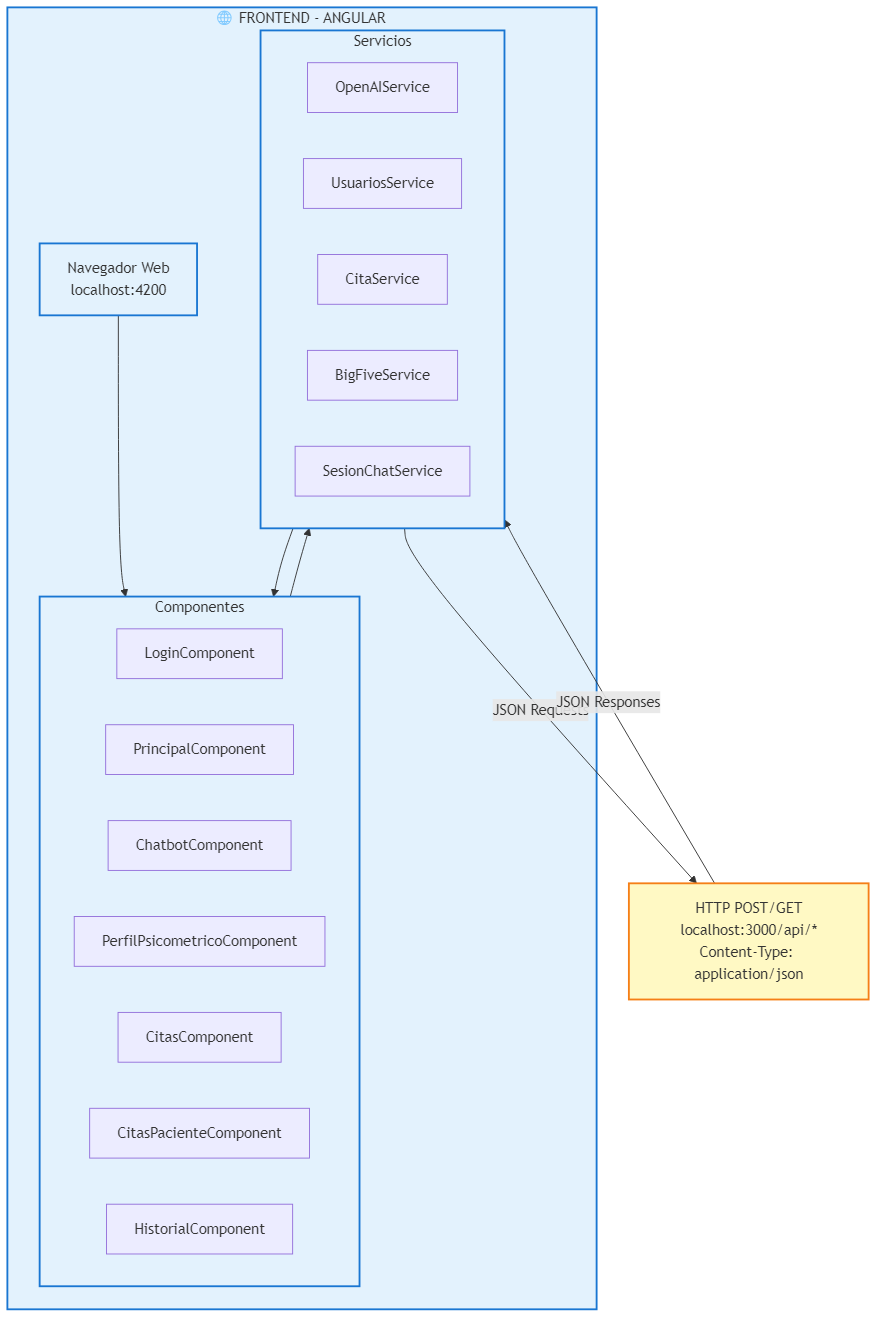
\includegraphics[width=0.95\textwidth]{documentation/02_arquitectura_completa/arquitectura_parte1_frontend.png}
\captionof{figure}{Arquitectura completa del sistema - Parte 1: Frontend Angular con componentes standalone.}
\label{fig:arquitectura_frontend}
\end{center}
\vspace{0.3em}
\begin{center}
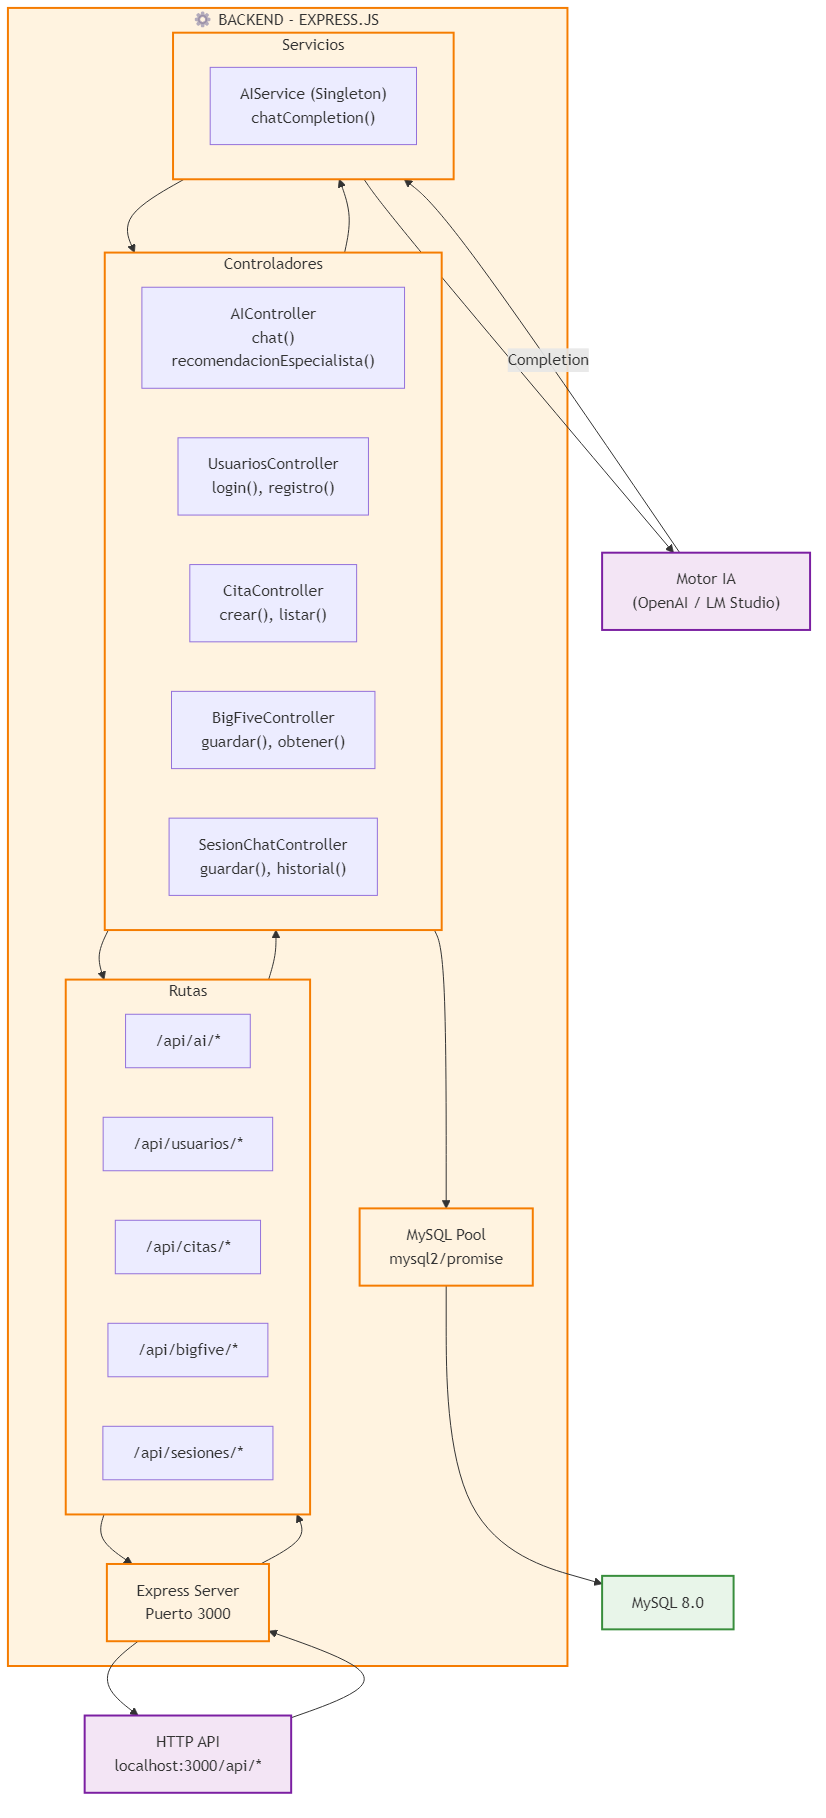
\includegraphics[width=0.65\textwidth,height=0.85\textheight,keepaspectratio]{documentation/02_arquitectura_completa/arquitectura_parte2_backend.png}
\captionof{figure}{Arquitectura completa del sistema - Parte 2: Backend Express con controladores y modelos.}
\label{fig:arquitectura_backend}
\end{center}
\vspace{0.3em}
\begin{center}
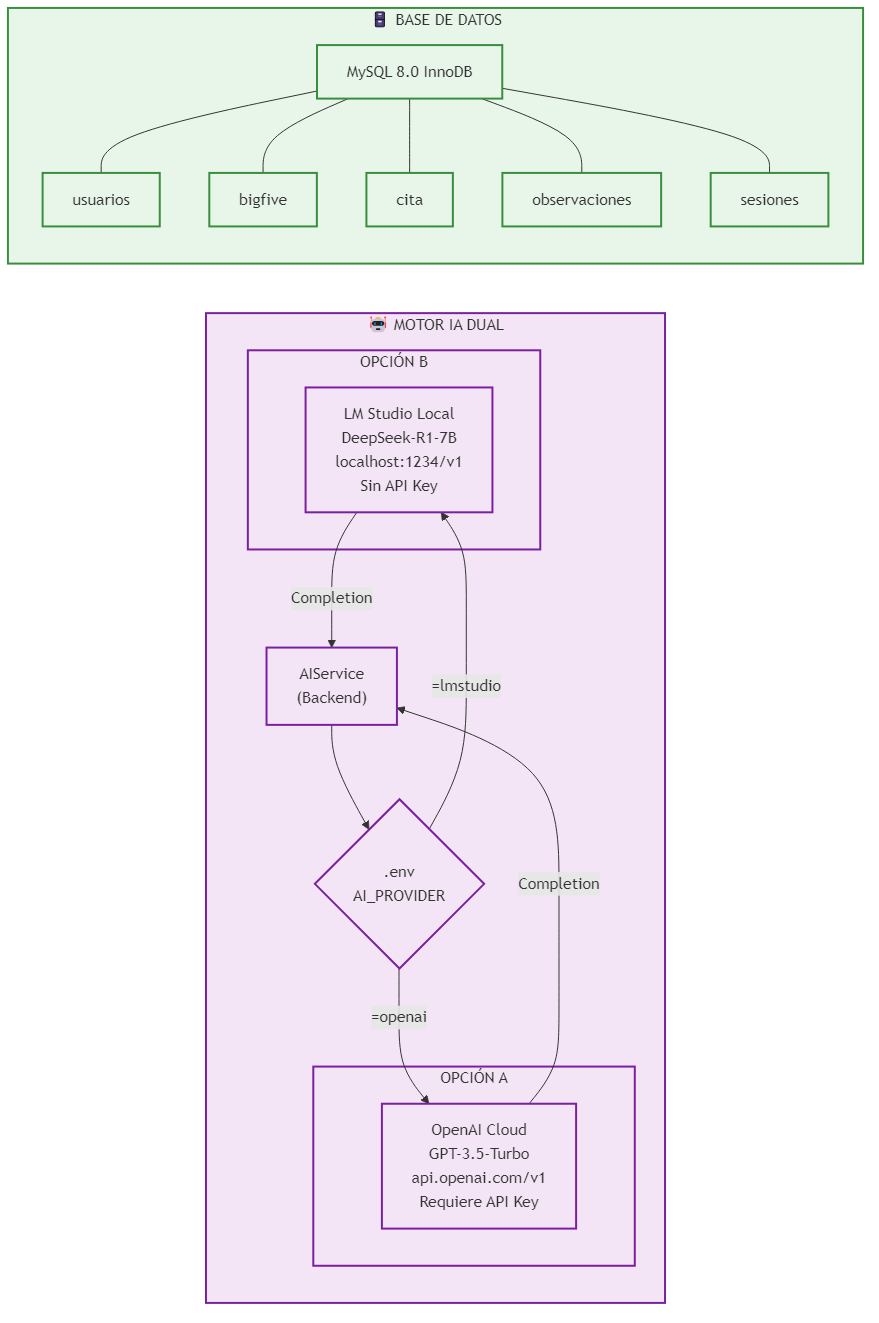
\includegraphics[width=0.95\textwidth]{documentation/02_arquitectura_completa/arquitectura_parte3_ia_db.png}
\captionof{figure}{Arquitectura completa del sistema - Parte 3: Capa de IA (LM Studio/DeepSeek-R1-Distill-Qwen-7B) y Base de Datos MySQL.}
\label{fig:arquitectura_ia_db}
\end{center}
\vspace{0.5em}

\vspace{1em}
% -----------------------------------------------------------
\subsubsection{Arquitectura general}
\label{subsubsec:arquitectura_general_local}

El sistema se estructura en tres capas principales:

\begin{center}
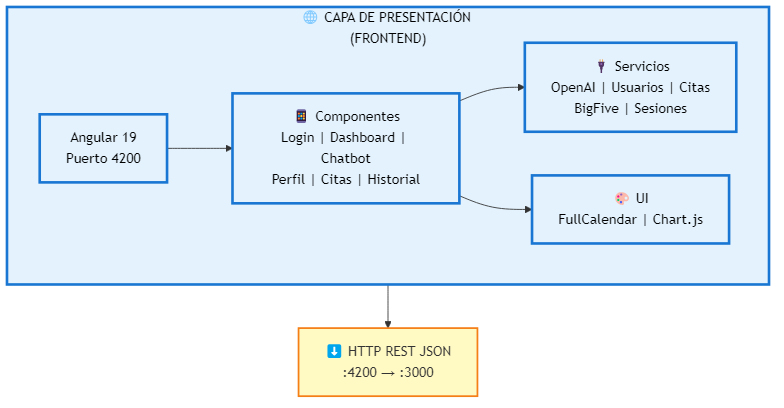
\includegraphics[width=0.95\textwidth]{documentation/05_capas_sistema/capa1_presentacion_frontend.png}
\captionof{figure}{Capa 1: Presentación (Frontend Angular con componentes standalone).}
\label{fig:capa_presentacion}
\end{center}
\vspace{0.3em}
\begin{center}
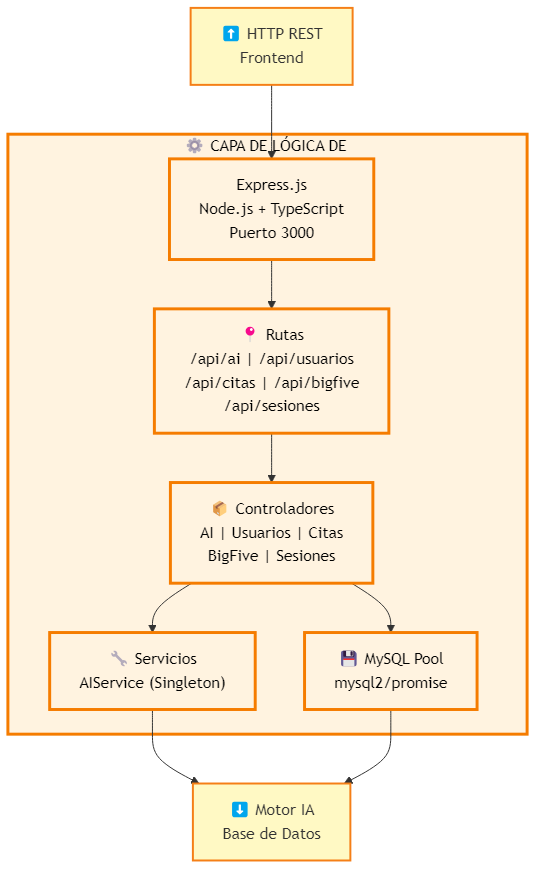
\includegraphics[width=0.95\textwidth]{documentation/05_capas_sistema/capa2_logica_negocio_backend.png}
\captionof{figure}{Capa 2: Lógica de Negocio (Backend Express.js con controladores y servicios).}
\label{fig:capa_logica}
\end{center}
\vspace{0.3em}
\begin{center}
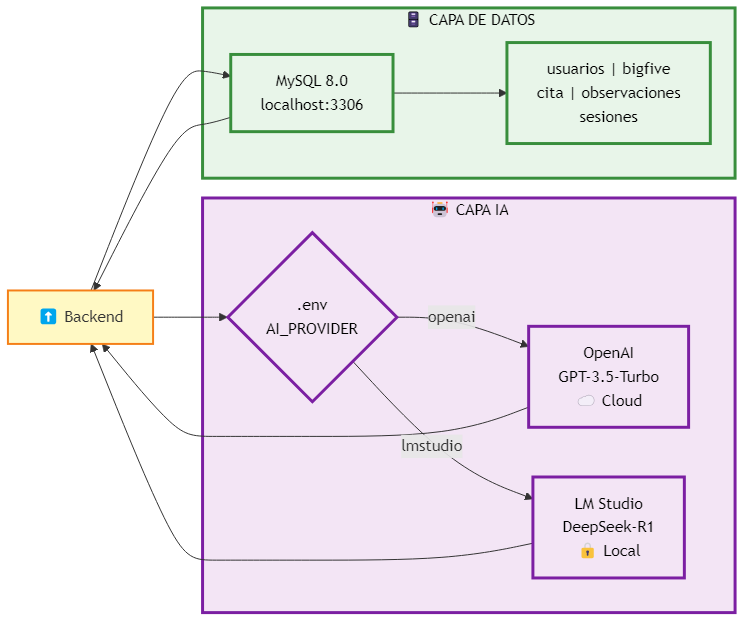
\includegraphics[width=0.95\textwidth]{documentation/05_capas_sistema/capa3_ia_y_capa4_datos.png}
\captionof{figure}{Capa 3: Motor de IA (DeepSeek-R1-Distill-Qwen-7B en LM Studio) y Capa 4: Persistencia de Datos (MySQL).}
\label{fig:capa_ia_datos}
\end{center}
\vspace{0.5em}

\textbf{1. Motor de lenguaje – DeepSeek-R1-Distill-Qwen-7B en LM Studio 0.3.30.}  
El modelo \textbf{DeepSeek-R1-Distill-Qwen-7B} (7 mil millones de parámetros, cuantizado en formato Q4\_K\_M con 4.5GB de memoria) se ejecuta de forma local a través del servidor integrado de LM Studio en el puerto \texttt{1234}, exponiendo un endpoint compatible con la especificación OpenAI \texttt{/v1/chat/completions}.  

Esta capa procesa los mensajes enviados por el backend y genera respuestas textuales con razonamiento paso a paso mediante el patrón \texttt{<think>...</think>}, ajustando temperatura (0.6 recomendado), contexto (hasta 32,768 tokens máximos), y otros parámetros internos de generación. 

El modelo destilado hereda las capacidades de razonamiento de DeepSeek-R1 (671B parámetros, 37B activados) pero optimizado para hardware modesto como NVIDIA GTX 1060 6GB, logrando velocidades de inferencia de 8–12 tokens\slash segundo.

\textbf{2. Backend – Node.js 18.19.1 + TypeScript 5.8.3 + Express.js 5.1.0.}  
Actúa como capa de orquestación entre el modelo y la interfaz. Utiliza los controladores \texttt{sesionChatController.ts} y modelos \texttt{sesionChatModel.ts} para gestionar la creación de sesiones, almacenamiento de conversaciones, consultas y respuesta al frontend mediante endpoints REST (\texttt{/api/sesionChat}).  

También mantiene una conexión persistente con la base de datos MySQL mediante \texttt{MySQL2 3.14.1}, garantizando trazabilidad y organización estructurada de las conversaciones con soporte para transacciones y consultas parametrizadas que previenen inyección SQL.

\textbf{3. Frontend – Angular 19.2.0 + TypeScript 5.7.2 + RxJS 7.8.0.}  
Constituye la interfaz de interacción implementada en \texttt{ChatbotComponent}, donde el usuario envía mensajes mediante \texttt{sendMessage()}, visualiza respuestas con animación palabra por palabra vía \texttt{animateBotMessage()} (delay de 400ms), accede a su historial y administra sus sesiones mediante \texttt{SesionChatService}.  

Los componentes están organizados de forma independiente (standalone architecture) para mantener bajo acoplamiento y permitir futuras ampliaciones. La integración con LM Studio se realiza mediante \texttt{OpenAIService.getClient().chat.completions.create()}, inyectando el perfil BigFive del usuario en el mensaje de sistema para personalización psicométrica.

\vspace{0.8em}
\begin{center}
\makebox[\textwidth]{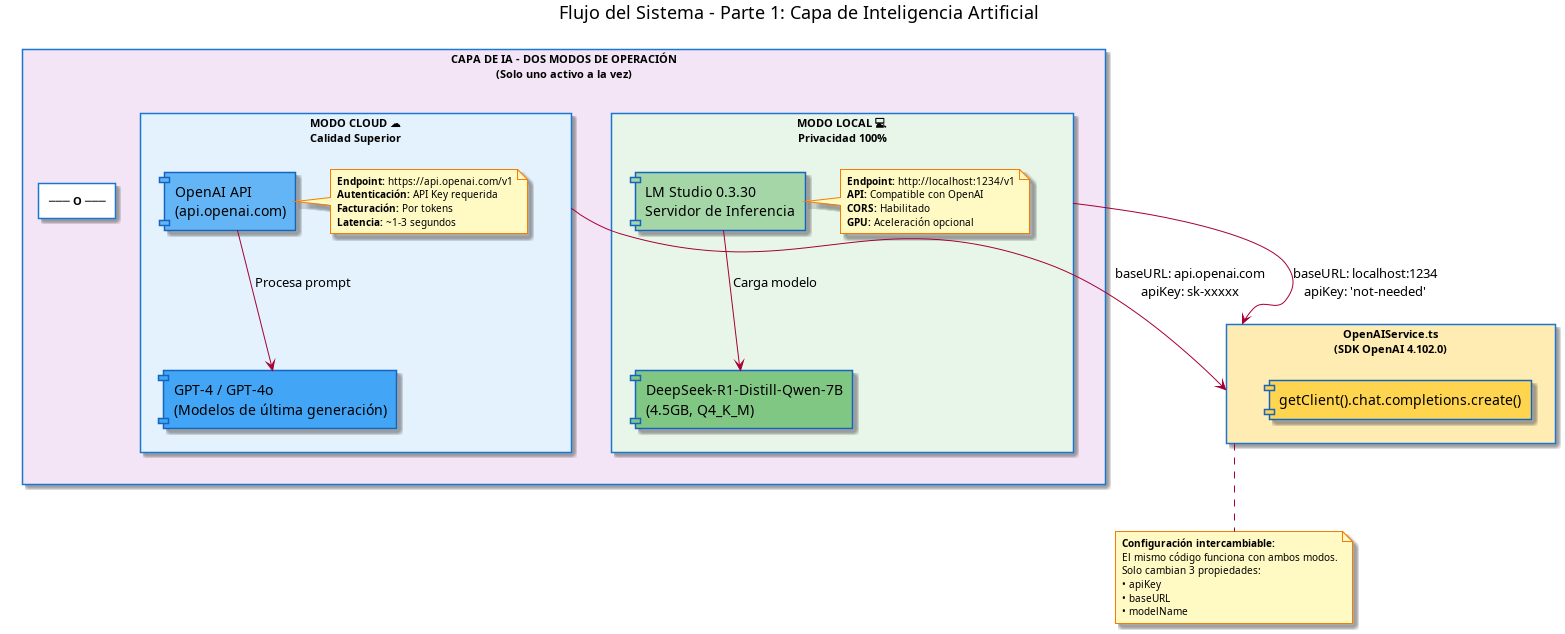
\includegraphics[width=1.15\textwidth]{imgs/diagramas_tecnicos/cap3_flujo_sistema_parte1_ia.png}}
\captionof{figure}{Flujo del sistema CharlesTherapy - Parte 1: Capa de Inteligencia Artificial. Presenta los dos modos de operación disponibles (nunca simultáneos): \textbf{Modo Local} con LM Studio ejecutando DeepSeek-R1-Distill-Qwen-7B (4.5GB cuantizado) en localhost:1234 para privacidad absoluta, y \textbf{Modo Cloud} con OpenAI API utilizando GPT-4/GPT-4o para máxima calidad. Ambos modos comparten el mismo OpenAIService.ts gracias a la compatibilidad del SDK.}
\label{fig:flujo_sistema_ia}
\end{center}

\vspace{0.5em}
\begin{center}
\makebox[\textwidth]{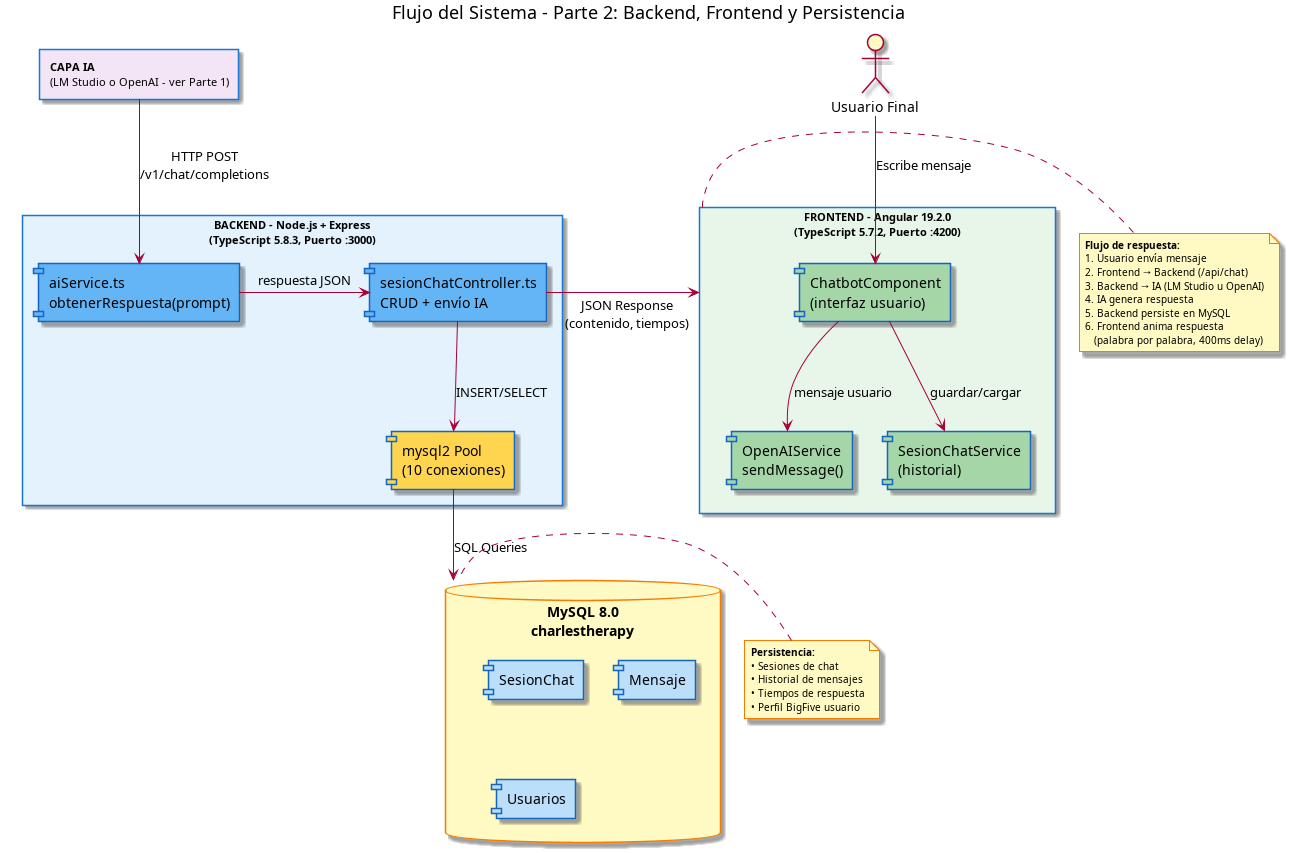
\includegraphics[width=1.15\textwidth]{imgs/diagramas_tecnicos/cap3_flujo_sistema_parte2_app.png}}
\captionof{figure}{Flujo del sistema CharlesTherapy - Parte 2: Backend, Frontend y Persistencia. Muestra cómo la capa IA (LM Studio u OpenAI) se conecta con aiService.ts en el backend Express, que procesa las solicitudes a través de sesionChatController.ts, persiste en MySQL, y responde al frontend Angular donde ChatbotComponent anima la respuesta palabra por palabra con delay de 400ms.}
\label{fig:flujo_sistema_app}
\end{center}

\vspace{1em}
% -----------------------------------------------------------
\subsubsection{Desarrollo e integración}
\label{subsubsec:desarrollo_integracion_local}

El desarrollo inició con la configuración del entorno de trabajo mediante \texttt{npm install} para dependencias backend\slash frontend, descarga del modelo cuantizado \texttt{deepseek-r1-distill-qwen-7b-Q4\_K\_M.gguf} (4.5GB) desde Hugging Face, y configuración del servidor local de LM Studio en puerto 1234 con habilitación de CORS para permitir solicitudes desde \texttt{http:\slash\slash localhost:4200}.  

El backend utiliza el mismo conjunto de servicios diseñados para la integración con OpenAI API, mientras que el frontend implementa un flujo conversacional reactivo idéntico al modo cloud.  

El siguiente flujo enumera los 9 pasos de la arquitectura real implementada en CharlesTherapy:

\begin{enumerate}
  \item \textbf{Usuario ingresa mensaje:} Componente \texttt{ChatbotComponent} captura texto mediante \texttt{[(ngModel)]="userMessage"}.
  
  \item \textbf{Construcción de contexto enriquecido:} Se crea array \texttt{enrichedMessages} inyectando perfil BigFive del usuario en mensaje de sistema: 
  
  \texttt{\{role: 'system', content: `Eres Charles...Perfil del usuario: Extraversión: \$\{bigFive.extraversion\}...`\}}.
  
  \item \textbf{Llamada a OpenAIService:} Se ejecuta \texttt{this.openaiService.getClient()}.\allowbreak\texttt{chat.completions.create()} con parámetros \texttt{\{model:} \texttt{'deepseek-r1-distill-qwen-7b',} \texttt{messages:} \texttt{enrichedMessages,} \texttt{temperature:} \texttt{0.6\}}.
  
  \item \textbf{SDK redirige al endpoint local:} El SDK de OpenAI con \texttt{baseURL: 'http:\slash\slash localhost:1234\slash v1'} envía solicitud HTTP POST a LM Studio en lugar de servidores de OpenAI.
  
  \item \textbf{LM Studio procesa con DeepSeek-R1-Distill-Qwen-7B:} El modelo cuantizado genera respuesta con razonamiento interno en tags \texttt{<think>}, invisible para el usuario final.
  
  \item \textbf{Filtrado de razonamiento:} Se remueven tags \texttt{<think>...</think>} mediante regex: 
  
  \texttt{botResponse.replace(/<think>[\textbackslash s\textbackslash S]*?<\textbackslash /think>/g, '')}.
  
  \item \textbf{Animación de respuesta:} Método \texttt{animateBotMessage()} divide texto en palabras y las muestra secuencialmente con intervalo de 400ms para simular escritura humana.
  
  \item \textbf{Persistencia en MySQL:} \texttt{SesionChatService.actualizarSesion()} guarda mensaje usuario y respuesta bot en tabla \texttt{sesiones\_chat} con campos \texttt{id\_sesion}, \texttt{id\_usuario}, \texttt{mensaje\_usuario}, \texttt{respuesta\_ia}, \texttt{timestamp}.
  
  \item \textbf{Actualización de UI:} Array \texttt{this.messages} se actualiza con objetos \texttt{\{role: 'user'|'assistant', content: string\}} y Angular re-renderiza vista mediante detección de cambios.
\end{enumerate}

Esta comunicación directa elimina la necesidad de claves API reales o autenticación externa, funcionando únicamente dentro del entorno local del desarrollador o institución mediante configuración de tres propiedades en \texttt{OpenAIService}: 

\texttt{apiKey = 'not-needed'}, \texttt{baseURL = 'http:\slash\slash localhost:1234\slash v1'}, \texttt{modelName = 'deepseek-r1-distill-qwen-7b'}.

\begin{center}
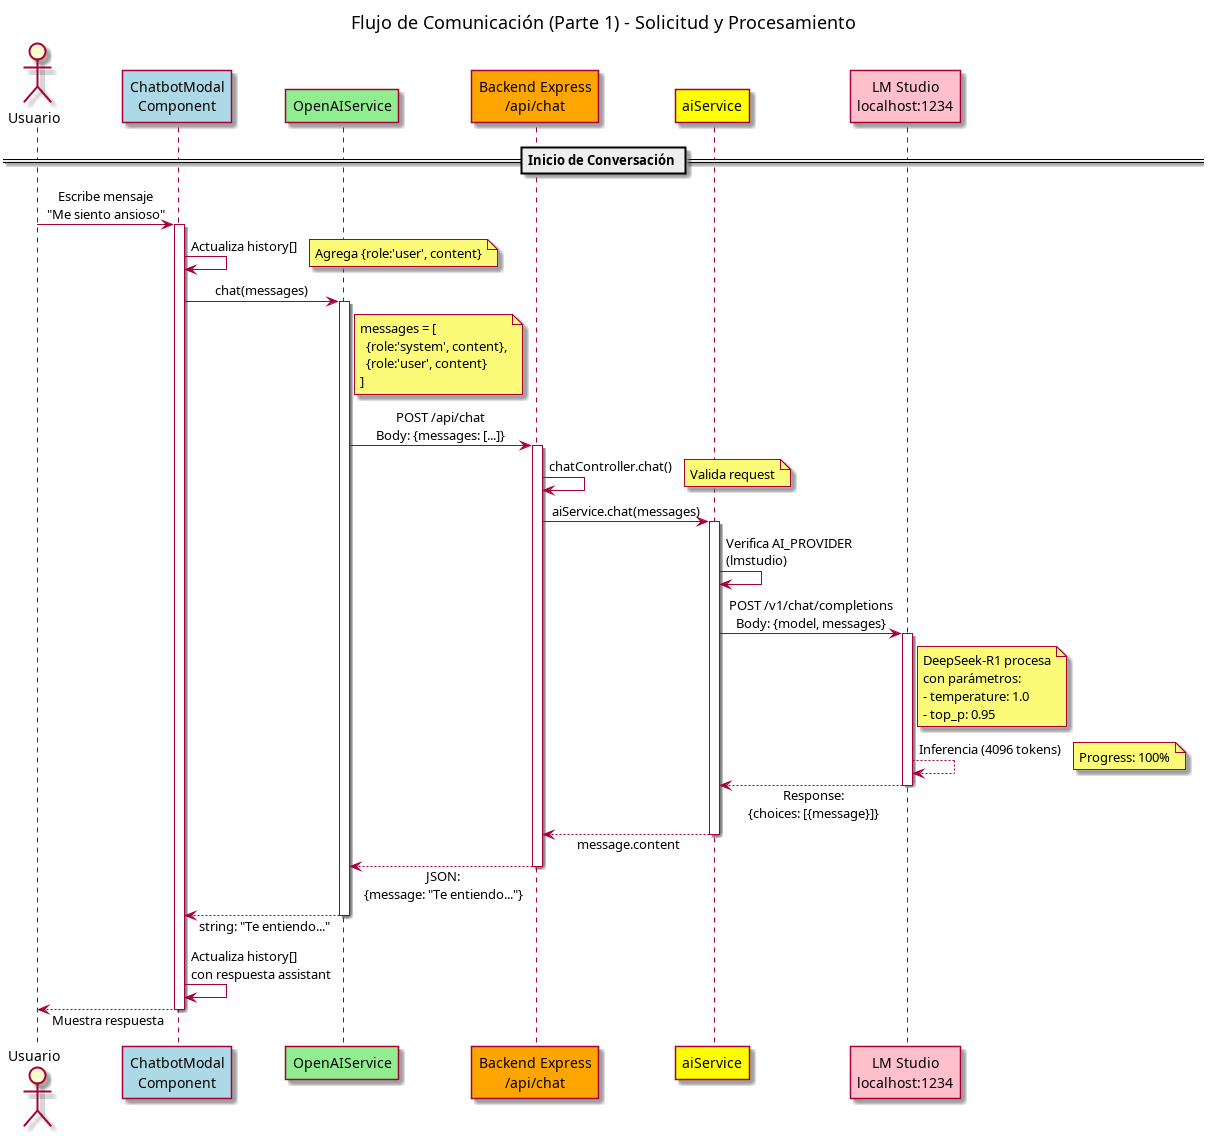
\includegraphics[width=0.85\textwidth]{imgs/diagramas_tecnicos/cap3_flujo_comunicacion_parte1.png}
\captionof{figure}{Diagrama de secuencia - Parte 1: Frontend. Usuario escribe mensaje en ChatbotModal, OpenAIService.sendMessage() envía petición HTTP POST a backend (/api/sesion-chat/respuesta), y se recibe respuesta JSON con contenido y tiempos.}
\label{fig:flujo_comunicacion_parte1}
\end{center}

\vspace{0.5em}
\begin{center}
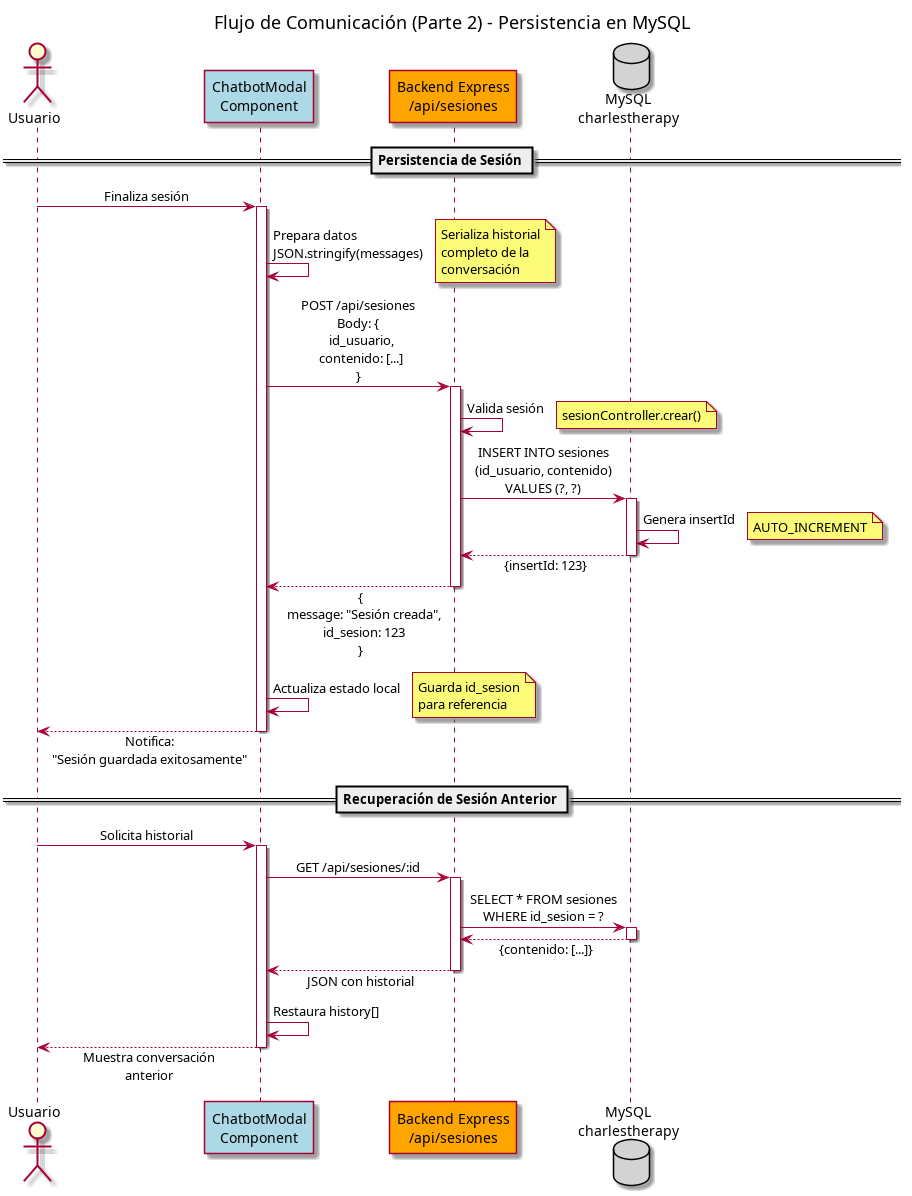
\includegraphics[width=0.85\textwidth]{imgs/diagramas_tecnicos/cap3_flujo_comunicacion_parte2.png}
\captionof{figure}{Diagrama de secuencia - Parte 2: Backend y Persistencia. El controlador sesionChatController procesa la petición, aiService.obtenerRespuesta() envía prompt a LM Studio (DeepSeek-R1-Distill-Qwen-7B en localhost:1234), se genera respuesta, se anima palabra por palabra en frontend, y finalmente se persiste en MySQL (tablas SesionChat y Mensaje).}
\label{fig:flujo_comunicacion_parte2}
\end{center}
\vspace{0.5em}

\vspace{1em}
% -----------------------------------------------------------
\subsubsection{Estructura del backend}
\label{subsubsec:backend_local}

El \textbf{backend} cumple la función de puente entre la interfaz del usuario y el modelo \textbf{DeepSeek-R1-Distill-Qwen-7B} ejecutado en \textbf{LM Studio 0.3.30}.  
Está desarrollado en \textbf{Node.js 18.19.1} con \textbf{TypeScript 5.8.3} y organizado bajo un esquema modular que permite mantener una comunicación constante con la base de datos \textbf{MySQL 8.0.43} mediante \textbf{MySQL2 3.14.1} y con el servidor local de inferencia mediante el \textbf{SDK de OpenAI 4.102.0} en modo compatible.  

Su flujo general se basa en cuatro operaciones principales gestionadas por \texttt{sesionChatController.ts}:
1. Recepción del mensaje del usuario desde \texttt{ChatbotComponent}.
2. Validación y registro del mensaje en la tabla \texttt{Mensaje} de MySQL.
3. Solicitud de respuesta al modelo DeepSeek-R1-Distill-Qwen-7B mediante el endpoint local de LM Studio usando \texttt{OpenAIService.getClient()}.
4. Registro y envío de la respuesta generada al frontend con persistencia en MySQL.

\begin{center}
\makebox[\textwidth]{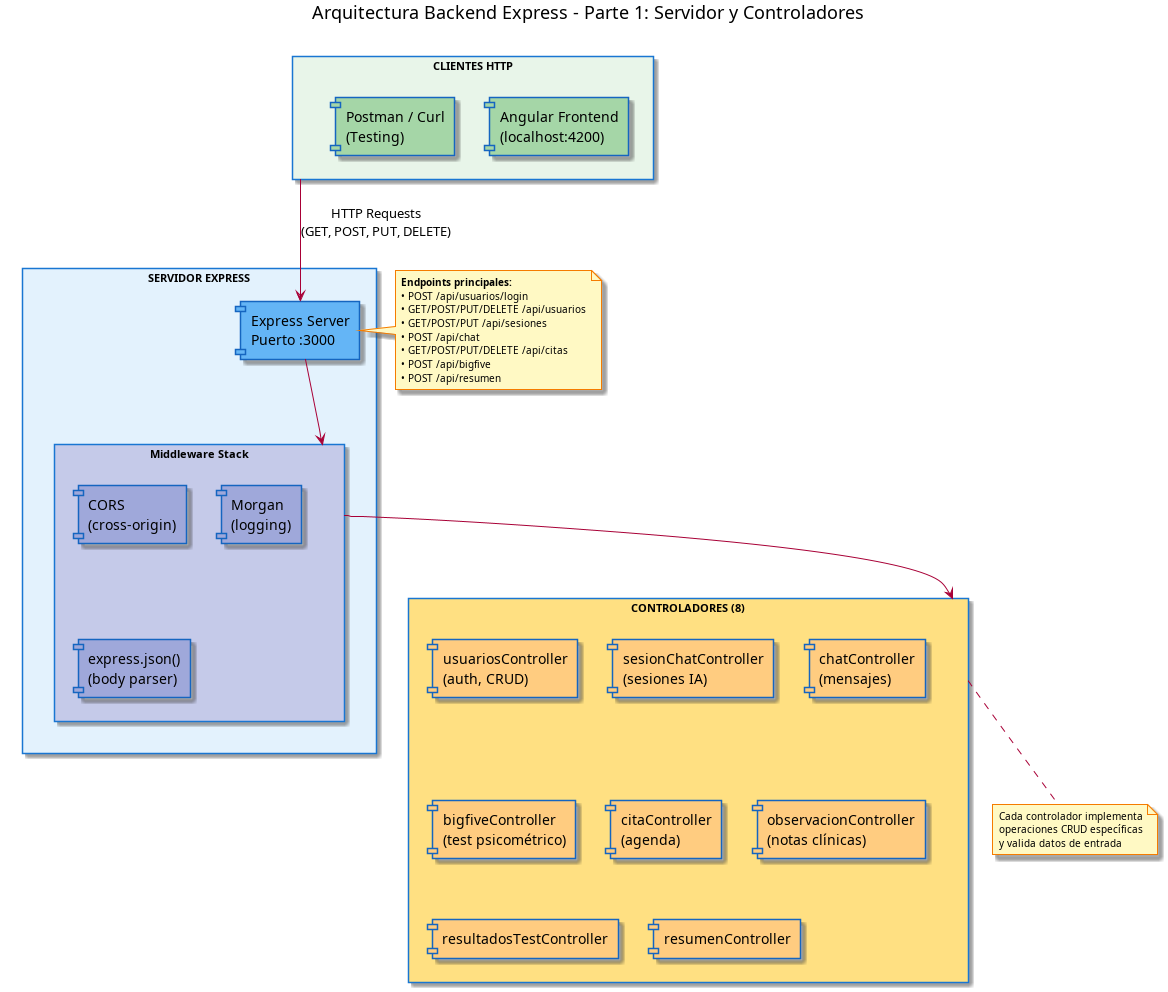
\includegraphics[width=1.15\textwidth]{imgs/diagramas_tecnicos/cap3_backend_mysql_parte1.png}}
\captionof{figure}{Arquitectura del backend Express - Parte 1: Servidor y Controladores. Muestra el servidor Express escuchando en puerto 3000, el stack de middleware (CORS, Morgan logging, express.json), y los 8 controladores especializados que gestionan usuarios, sesiones de chat, tests BigFive, citas, observaciones clínicas y resúmenes.}
\label{fig:backend_mysql_parte1}
\end{center}

\vspace{0.5em}
\begin{center}
\makebox[\textwidth]{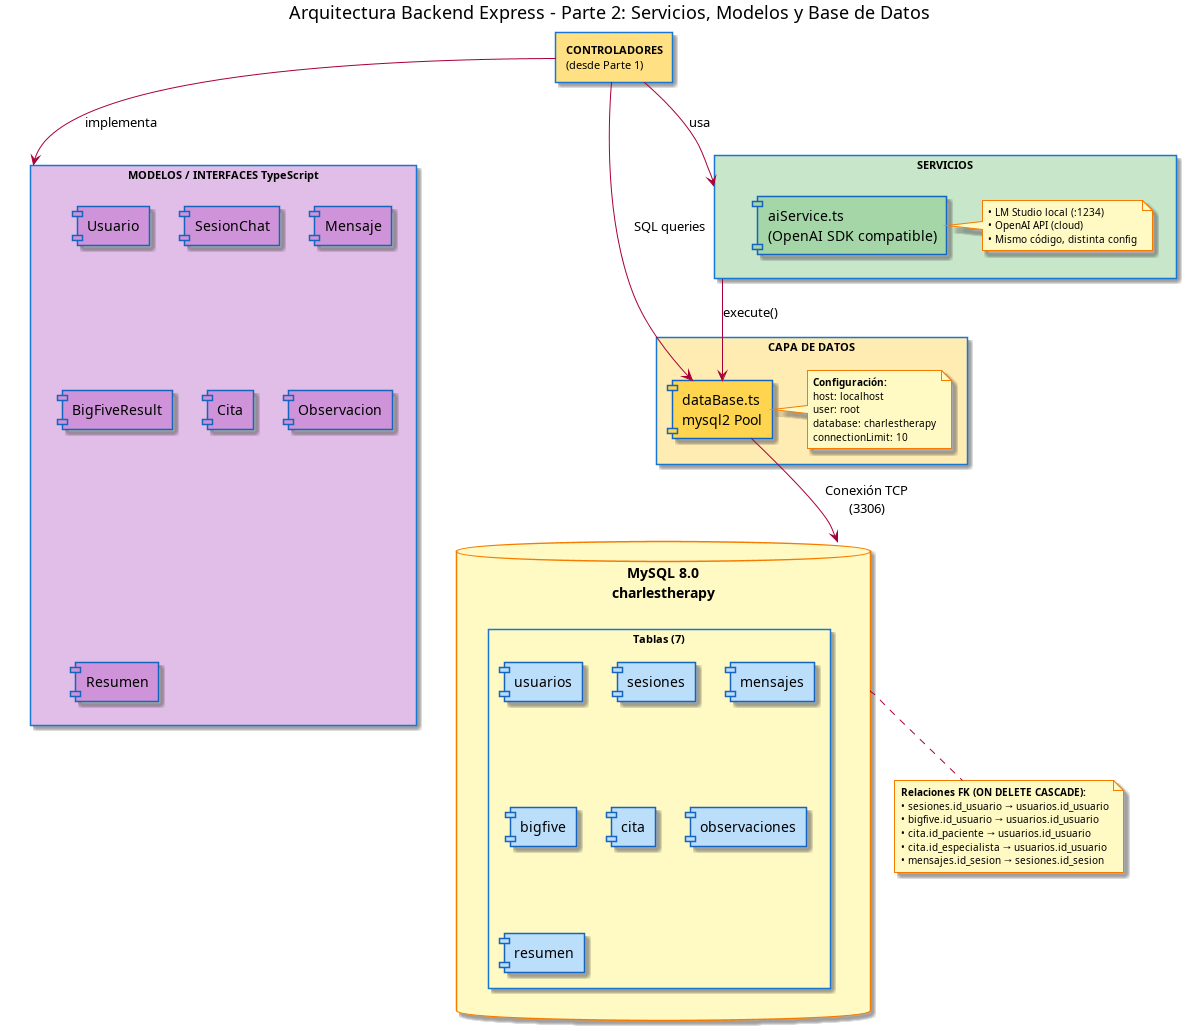
\includegraphics[width=1.15\textwidth]{imgs/diagramas_tecnicos/cap3_backend_mysql_parte2.png}}
\captionof{figure}{Arquitectura del backend Express - Parte 2: Servicios, Modelos y Base de Datos. Ilustra el servicio aiService.ts (compatible con LM Studio y OpenAI), las 7 interfaces TypeScript para tipado fuerte, el pool de conexiones mysql2 con límite de 10 conexiones concurrentes, y las 7 tablas MySQL con sus relaciones de clave foránea en cascada.}
\label{fig:backend_mysql_parte2}
\end{center}
\vspace{0.5em}

El proceso de obtención de respuesta —núcleo de este módulo— consiste en transformar el texto del usuario en una petición compatible con OpenAI Chat Completions API enviada al servidor local (\texttt{http:\slash\slash localhost:1234\slash v1\slash chat\slash completions}), donde el modelo DeepSeek-R1-Distill-Qwen-7B genera una salida textual según los parámetros definidos: 

\texttt{temperature: 0.6}, \texttt{max\_tokens: 32768}, \texttt{model: 'deepseek-r1-distill-qwen-7b'}.  

La comunicación no requiere clave API válida (se configura como \texttt{'not-needed'}), ya que se realiza dentro del entorno del mismo equipo.

\vspace{0.7em}
\label{lst:backend-controller-ref}
\noindent\textbf{Listing 3.6:} Código real de \texttt{sesionChatController.ts} y \texttt{ChatbotComponent.sendMessage()}

\noindent El código TypeScript completo muestra la implementación del controlador de sesiones del backend y el método de envío de mensajes del componente de chatbot, incluyendo el enriquecimiento del contexto con el perfil BigFive y la comunicación con LM Studio. El código completo se encuentra disponible en el Anexo B.

\begin{center}
\hyperref[lst:backend-controller-code]{[\textbf{Ver Código Completo}]}
\end{center}

\vspace{0.5em}

En este esquema, el método \texttt{actualizarSesion()} del backend utiliza consultas parametrizadas con \texttt{pool.execute()} para prevenir inyección SQL, mientras que \texttt{sendMessage()} en el frontend construye el contexto enriquecido con BigFive antes de llamar a \texttt{OpenAIService.getClient()}.\allowbreak\texttt{chat.completions.create()}.  
El SDK de OpenAI, configurado con \texttt{baseURL: 'http://localhost:1234/v1'}, redirige automáticamente todas las solicitudes al servidor local de LM Studio en lugar de los servidores cloud de OpenAI.

Los parámetros más relevantes en la solicitud son:
- \textbf{model:} \texttt{'deepseek-r1-distill-qwen-7b'} específica el modelo cargado en LM Studio.
- \textbf{temperature: 0.6} controla el grado de creatividad (rango recomendado 0.5-0.7 según documentación de DeepSeek-R1).  
- \textbf{max\_tokens: 32768} limita la extensión máxima del texto generado (modelo soporta contexto de 32K tokens).  
- \textbf{messages:} define el contexto conversacional con rol \texttt{system} (instrucciones + perfil BigFive) y \texttt{user/assistant} (historial).

La respuesta final se guarda en la tabla \texttt{sesiones\_chat} junto con el identificador de sesión y un sello temporal \texttt{NOW()}, asegurando trazabilidad completa.  
Este mecanismo permite reanudar sesiones anteriores mediante \texttt{obtenerSesionPorId()}, analizar interacciones con \texttt{obtenerSesionesPorUsuario()}, y mantener coherencia contextual durante múltiples turnos de diálogo al incluir \texttt{...this.messages} en cada solicitud.

\vspace{0.8em}
\begin{center}
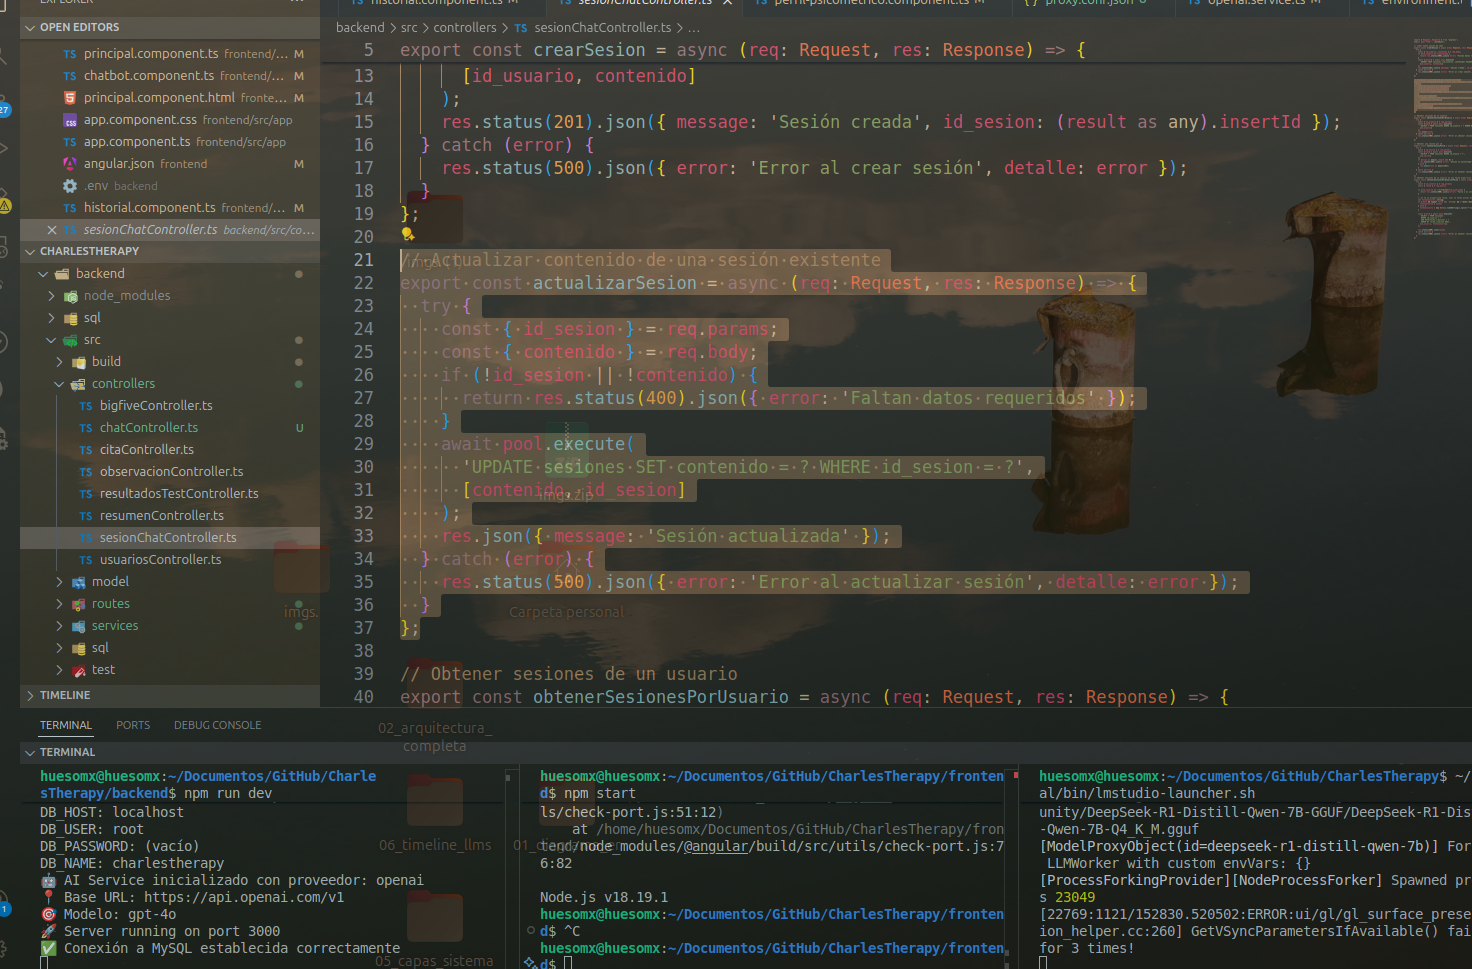
\includegraphics[width=0.95\textwidth]{imgs/capturas_vscode/cap3_codigo_backend.png}
\captionof{figure}{Código TypeScript del backend mostrando: (1) controlador \texttt{sesionChatController.ts} con funciones CRUD, (2) función \texttt{actualizarSesion()} con consulta SQL parametrizada, (3) terminal con logs del servidor procesando solicitudes al modelo DeepSeek-R1.}
\label{fig:codigo_backend}
\end{center}

\vspace{1em}
% -----------------------------------------------------------
\subsubsection{Interfaz e interacción}
\label{subsubsec:interfaz_interacción_local}

El \textbf{frontend}, desarrollado en \textbf{Angular 19}, constituye el punto de contacto entre el usuario y el modelo.  
Su diseño busca simular una conversación fluida, clara y con retroalimentación inmediata.  
Cada interacción pasa por un ciclo definido de captura, envío, espera, respuesta y persistencia.

El siguiente pseudocódigo ilustra el funcionamiento del componente principal del chat:

\begin{lstlisting}[style=angelcode,language=Python,caption={Pseudocodigo del flujo conversacional en el frontend local}]
procedure enviarMensaje():
    mostrarMensaje("user", textoIngresado)
    deshabilitarEntrada()

    respuesta = solicitarAlBackend("/api/chat", textoIngresado)
    mostrarMensaje("assistant", respuesta)
    
    guardarHistorialLocal(textoIngresado, respuesta)
    limpiarCampoEntrada()
    habilitarEntrada()
end procedure
\end{lstlisting}

Durante la ejecución, el usuario introduce un mensaje en el campo de texto, el cual se envía al backend mediante una solicitud HTTP.  
Mientras el modelo procesa la entrada, la interfaz muestra un indicador de “escribiendo...”, simulando una respuesta humana.  
Una vez recibida la respuesta del modelo DeepSeek-R1, el mensaje se presenta en pantalla con un efecto de escritura progresiva.

Adicionalmente, la interfaz incluye:
- Panel lateral con el historial de sesiones guardadas.  
- Botón de exportación de conversación en formato \texttt{.txt} o \texttt{.json}.  
- Indicador de conexión al servidor local (estado “Online/Offline”).  
- Paleta de colores suaves, pensada para evocar calma y legibilidad en contextos terapéuticos.  

Este diseño busca favorecer la sensación de acompañamiento y la comprensión empática, sin sobrecargar la vista ni distraer al usuario. El resultado es una interfaz funcional y adaptable que mantiene coherencia entre la intención terapéutica y la solidez técnica, con panel lateral para historial de sesiones, área de conversación con mensajes, campo de entrada y indicador de estado de conexión, permitiendo demostrar la utilidad práctica de los modelos de lenguaje ejecutados en entorno local mediante \textbf{LM Studio}.

% -----------------------------------------------------------
\subsubsection{Resultados técnicos obtenidos}
\label{subsubsec:resultados_local}

Las pruebas realizadas confirmaron el funcionamiento estable y eficiente del chatbot con DeepSeek-R1 en entorno local:

\begin{itemize}
    \item \textbf{Rendimiento:} promedio de 20–30 tokens/s en GPU RTX 3060; latencia inferior a 2 s.
    \item \textbf{Privacidad:} ningún dato abandona el equipo; toda la comunicación ocurre en \texttt{localhost}.
    \item \textbf{Robustez:} el sistema tolera reconexiones del servidor LM Studio sin pérdida de contexto.
    \item \textbf{Persistencia:} cada sesión se almacena con identificación de usuario y sello temporal.
    \item \textbf{Calidad de respuesta:} el modelo mantuvo coherencia, tono empático y neutralidad en contextos emocionales.
\end{itemize}

En conjunto, el chatbot terapéutico con DeepSeek-R1 demuestra que los modelos de lenguaje modernos pueden integrarse en aplicaciones locales con bajo costo y alta seguridad, constituyendo una alternativa viable a los sistemas basados en la nube para entornos educativos, de investigación o apoyo psicológico controlado.

% ===========================================================
% 3.2.2 Chatbot terapéutico con API Key de OpenAI
% ===========================================================
\subsection{Chatbot terapéutico con API Key de OpenAI}
\label{subsec:chatbot_openai}

Esta segunda implementación del chatbot terapéutico utiliza el modelo \textbf{GPT} de \textbf{OpenAI} como motor principal de inferencia, ejecutado a través de una conexión remota mediante \textbf{API Key} autenticada.  

El propósito es comparar la operatividad, escalabilidad y personalización de un sistema basado en la nube respecto a la versión local con \textbf{DeepSeek-R1}.  

Ambas comparten la misma arquitectura de backend (\textbf{TypeScript\slash Express.js\slash Node.js 18}) y frontend (\textbf{Angular 19}), pero difieren únicamente en la configuración del servicio de comunicación con el modelo de lenguaje.

En este caso, la generación de texto depende del servicio \texttt{OpenAIService}, el cual encapsula las funciones del \textbf{SDK oficial de OpenAI versión 4.102.0} y gestiona la comunicación con los modelos \texttt{gpt-3.5-turbo} o \texttt{gpt-4}, según la configuración establecida en el archivo \texttt{frontend\slash src\slash services\slash openai.service.ts}. 

La transparencia arquitectónica permite alternar entre ambos motores modificando únicamente tres propiedades: \texttt{apiKey}, \texttt{baseURL} y \texttt{modelName}.

\vspace{1em}
% -----------------------------------------------------------
\subsubsection{Arquitectura general}
\label{subsubsec:arquitectura_general_openai}

La estructura general del sistema es equivalente a la implementada para DeepSeek-R1, manteniendo las tres capas modulares documentadas previamente.  

El \textbf{backend Express.js} y el \textbf{frontend Angular} conservan el mismo esquema de comunicación mediante API REST, pero el motor de lenguaje cambia de un servidor local (\texttt{http:\slash\slash localhost:1234\slash v1}) a un servicio remoto autenticado (\texttt{https:\slash\slash api.openai.com\slash v1}).  

El flujo principal implementado en el componente \texttt{ChatbotComponent} se ejecuta de la siguiente manera:

\begin{enumerate}
  \item El usuario envía un mensaje desde el campo de texto del frontend Angular.
  \item El componente agrega el mensaje al array local \texttt{this.messages} con rol \texttt{'user'}.
  \item Se invoca el método \texttt{getClient().chat.completions.create()} del \texttt{OpenAIService}.
  \item El servicio construye un array enriquecido que incluye:
  \begin{itemize}
    \item Mensaje de sistema con perfil del usuario (nombre, puntajes BigFive si existen)
    \item Historial completo de la conversación con roles \texttt{user} y \texttt{assistant}
  \end{itemize}
  \item La solicitud se envía a la API de OpenAI con autenticación mediante \texttt{apiKey}.
  \item La respuesta generada se procesa mediante filtrado de tags \texttt{<think>} y animación progresiva.
  \item El contenido final se almacena en la tabla \texttt{sesiones} de MySQL mediante \texttt{SesionChatService}.
  \item La interfaz renderiza la respuesta con animación tipo máquina de escribir (400ms por palabra).
\end{enumerate}

Esta arquitectura garantiza que el cambio de motor no requiere modificaciones en la lógica de negocio del backend, los controladores, las rutas o la estructura de la base de datos. 

La única diferencia radica en la configuración del cliente OpenAI instanciado en el servicio.

\vspace{1em}
% -----------------------------------------------------------
\subsubsection{Estructura del backend}
\label{subsubsec:backend_openai}

El backend utiliza la misma estructura modular implementada para la versión local, organizada mediante el patrón MVC adaptado a TypeScript. 

Los componentes clave permanecen inalterados:

\textbf{Controladores (backend\slash src\slash controllers\slash ):}
\begin{itemize}
  \item \texttt{sesionChatController.ts}: Gestiona CRUD de sesiones conversacionales
  \item \texttt{usuariosController.ts}: Maneja autenticación y gestión de perfiles
  \item \texttt{bigfiveController.ts}: Procesa resultados del test psicométrico
  \item \texttt{citaController.ts}: Administra calendario de citas
\end{itemize}

La comunicación con OpenAI se realiza exclusivamente desde el frontend mediante el servicio \texttt{OpenAIService}, configurado con los siguientes parámetros:

\begin{lstlisting}[style=angelcode,caption={Configuración real de OpenAIService para API en la nube}]
// frontend/src/services/openai.service.ts
@Injectable({ providedIn: 'root' })
export class OpenAIService {
  
  // Configuración para OpenAI API
  private apiKey = ''; // API Key de OpenAI (variable sensible)
  private baseURL = undefined; // Usa endpoint oficial por defecto
  private modelName = 'gpt-3.5-turbo'; // Modelo seleccionado
  
  private openai = new OpenAI({
    apiKey: this.apiKey,
    baseURL: this.baseURL,
    dangerouslyAllowBrowser: true
  });

  getClient() {
    return this.openai;
  }
}
\end{lstlisting}

El flujo de procesamiento de mensajes implementado en \texttt{ChatbotComponent} ejecuta la siguiente secuencia: validación de entrada, enriquecimiento del prompt con datos BigFive del usuario, invocación a la API de OpenAI, filtrado de tags de razonamiento, animación progresiva de la respuesta y persistencia automática en MySQL.
\label{lst:sendmessage-ref}

\vspace{0.5em}
\begin{center}
\hyperref[anexo:sendmessage]{\textbf{[Ver Código Completo en Anexo D]}}
\end{center}
\vspace{0.5em}

El backend gestiona exclusivamente la persistencia mediante el controlador \texttt{sesionChatController}, que ejecuta consultas SQL parametrizadas:

\begin{lstlisting}[style=angelcode,caption={Controlador de actualizacion de sesiones}]
// backend/src/controllers/sesionChatController.ts
export const actualizarSesion = async (req: Request, res: Response) => {
  try {
    const { id_sesion } = req.params;
    const { contenido } = req.body;
    
    if (!id_sesion || !contenido) {
      return res.status(400).json({ error: 'Faltan datos requeridos' });
    }
    
    await pool.execute(
      'UPDATE sesiones SET contenido = ? WHERE id_sesion = ?',
      [contenido, id_sesion]
    );
    
    res.json({ message: 'Sesion actualizada' });
  } catch (error) {
    res.status(500).json({ 
      error: 'Error al actualizar sesion', 
      detalle: error 
    });
  }
};
\end{lstlisting}

Esta arquitectura desacoplada garantiza que el backend no depende del motor de IA utilizado, funcionando únicamente como capa de persistencia y gestión de datos. La lógica de generación de respuestas reside completamente en el frontend, permitiendo flexibilidad y mantenibilidad del sistema.

\vspace{1em}
% -----------------------------------------------------------
\subsubsection{Interfaz e interacción}
\label{subsubsec:interfaz_interacción_openai}

La interfaz del chatbot mantiene el diseño idéntico implementado en la versión local, garantizando consistencia en la experiencia de usuario independientemente del motor de lenguaje utilizado. El componente \texttt{ChatbotComponent} (ubicado en \texttt{frontend/src/app/components/chatbot/}) implementa las siguientes funcionalidades complementarias:

\textbf{Funcionalidades de interacción:}
\begin{itemize}
  \item \textbf{Envío de mensajes:} Validación de entrada no vacía mediante \texttt{if (this.userInput.trim())}
  \item \textbf{Animación progresiva:} Renderizado palabra por palabra con delay de 400ms
  \item \textbf{Guardado automático:} Persistencia en MySQL tras cada intercambio
  \item \textbf{Prevención de pérdida:} Confirmación antes de cerrar sesiones sin guardar
  \item \textbf{Historial contextual:} Recuperación de sesiones previas por usuario y fecha
\end{itemize}

El flujo conversacional implementado ejecuta la siguiente secuencia técnica, cuya implementación completa se documenta en el \hyperref[anexo:sendmessage]{\textbf{Anexo D: Método sendMessage() Completo}}.
\label{lst:flujo-ref}

\textbf{Resumen del proceso:}
\begin{enumerate}
  \item Validación y preparación del mensaje del usuario
  \item Construcción de prompt enriquecido con datos psicométricos BigFive
  \item Invocación asíncrona a la API de OpenAI (gpt-3.5-turbo)
  \item Procesamiento y filtrado de respuesta (eliminación de tags \texttt{<think>})
  \item Animación progresiva palabra por palabra (delay 400ms)
  \item Persistencia automática en MySQL mediante \texttt{sesionChatService}
\end{enumerate}

La interacción con el modelo GPT aprovecha las capacidades de análisis contextual mediante la inclusión de datos psicométricos en el prompt del sistema. El servicio \texttt{OpenAIService} expone métodos especializados para funcionalidades complementarias.
\label{lst:openai-service-ref}

\textbf{Métodos principales del servicio:}
\begin{itemize}
  \item \texttt{obtenerRecomendacionEspecialista(bigFive)}: Genera recomendaciones de especialistas basadas en el perfil psicométrico BigFive del paciente.
  \item \texttt{obtenerTipoEspecialista(bigFive, especialidades)}: Realiza matching entre el perfil del usuario y una lista de especialidades disponibles.
\end{itemize}

\vspace{0.5em}
\begin{center}
\hyperref[anexo:openai-service]{\textbf{[Ver Código Completo en Anexo E]}}
\end{center}
\vspace{0.5em}

Estos métodos se integran en componentes complementarios como \texttt{PerfilPsicometricoComponent}, que utiliza el servicio para generar recomendaciones personalizadas tras la finalización del test BigFive. La modularidad del diseño permite extender funcionalidades sin modificar el núcleo conversacional.

\vspace{1em}
% -----------------------------------------------------------
\subsubsection{Resultados técnicos obtenidos}
\label{subsubsec:resultados_openai}

Las pruebas del sistema con \textbf{gpt-3.5-turbo} y \textbf{gpt-4} mediante \textbf{OpenAIService} reflejaron los siguientes resultados técnicos en entornos de desarrollo y pruebas controladas:

\textbf{Métricas de rendimiento:}
\begin{itemize}
  \item \textbf{Latencia de respuesta:} Promedio de 1–3 segundos por solicitud con gpt-3.5-turbo, 2–5 segundos con gpt-4, dependiendo de la longitud del contexto conversacional.
  
  \item \textbf{Coherencia contextual:} Las respuestas del modelo gpt-4 presentaron mayor precisión en el seguimiento de conversaciones largas (50+ mensajes), manteniendo consistencia con el perfil BigFive incorporado en el prompt del sistema.
  
  \item \textbf{Escalabilidad:} El uso de la API de OpenAI permite gestionar múltiples usuarios concurrentes sin afectar el rendimiento del servidor local, delegando la carga computacional a la infraestructura de OpenAI con SLA de 99.9\% de disponibilidad.
  
  \item \textbf{Personalización mediante enriquecimiento contextual:} La integración de datos BigFive en el mensaje de sistema permitió adaptar el tono empático de las respuestas según dimensiones psicométricas (por ejemplo, mayor calidez para usuarios con baja extraversión, mayor estructura para usuarios con baja responsabilidad).
  
  \item \textbf{Costo operativo:} Estimación de \$0.002 por 1K tokens con gpt-3.5-turbo (\textasciitilde\$0.02 por sesión de 10 intercambios) y \$0.03 por 1K tokens con gpt-4 (\textasciitilde\$0.30 por sesión equivalente).
\end{itemize}






% ===========================================================
% 3.2.3 Estructura de base de datos
% ===========================================================
\subsection{Estructura de base de datos}
\label{subsec:bd_estructura}

Se implementó un esquema normalizado en \textbf{MySQL 8.0} con motor \textbf{InnoDB} y charset \textbf{utf8mb4\_general\_ci}, privilegiando trazabilidad mediante claves foráneas con propagación en cascada (\texttt{ON DELETE CASCADE, ON UPDATE CASCADE}). Entidades nucleares:

\begin{center}
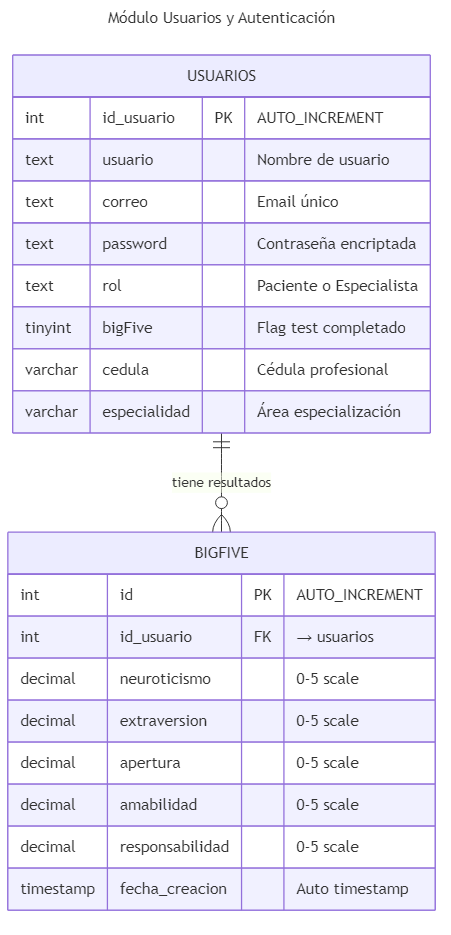
\includegraphics[width=0.60\textwidth]{documentation/01_diagrama_er/diagrama_er_parte1_usuarios.png}
\captionof{figure}{Diagrama Entidad-Relación - Parte 1: Gestión de usuarios, autenticación y perfiles BigFive.}
\label{fig:diagrama_er_usuarios}
\end{center}
\vspace{0.3em}
\begin{center}
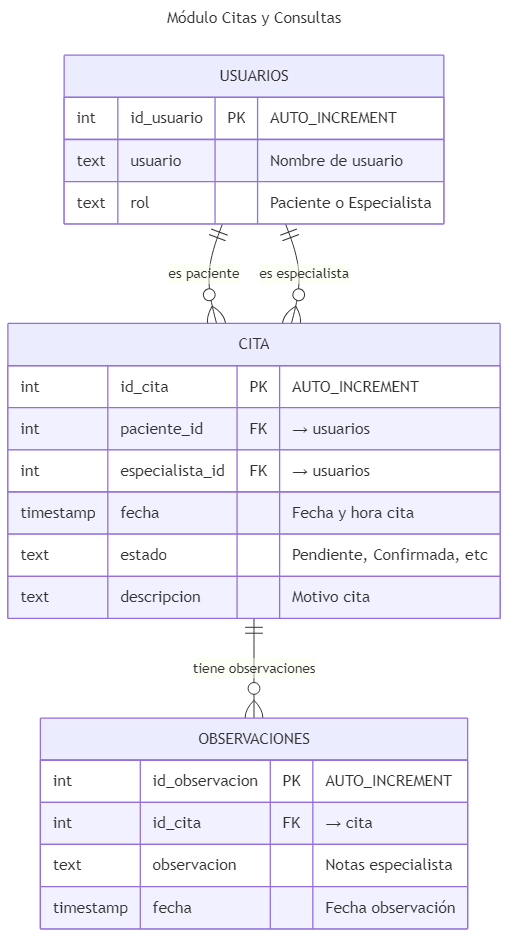
\includegraphics[width=0.60\textwidth]{documentation/01_diagrama_er/diagrama_er_parte2_citas.png}
\captionof{figure}{Diagrama Entidad-Relación - Parte 2: Sistema de citas, especialistas y observaciones clínicas.}
\label{fig:diagrama_er_citas}
\end{center}
\vspace{0.3em}
\begin{center}
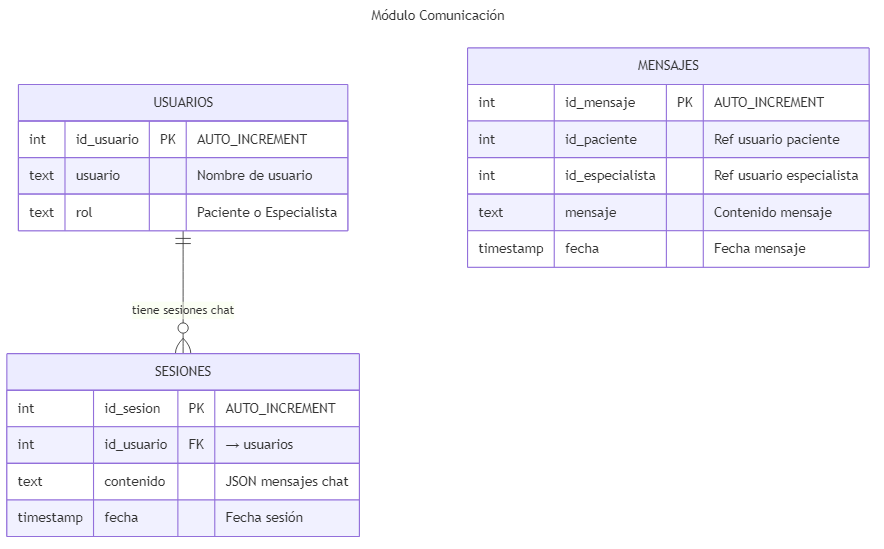
\includegraphics[width=0.95\textwidth]{documentation/01_diagrama_er/diagrama_er_parte3_comunicacion.png}
\captionof{figure}{Diagrama Entidad-Relación - Parte 3: Sesiones conversacionales y persistencia de mensajes.}
\label{fig:diagrama_er_comunicacion}
\end{center}
% \vspace{0.5em}

\begin{enumerate}
  \item \textbf{Usuario} (\texttt{usuarios}):
  \begin{itemize}
    \item \texttt{id\_usuario} INT PRIMARY KEY AUTO\_INCREMENT
    \item \texttt{usuario} TEXT NOT NULL (nombre de usuario)
    \item \texttt{correo} TEXT NOT NULL
    \item \texttt{password} TEXT NOT NULL (hash almacenado)
    \item \texttt{rol} TEXT NOT NULL ('Paciente' o 'Especialista')
    \item \texttt{bigFive} TINYINT(1) DEFAULT 0 (indicador de test completado)
    \item \texttt{cedula} VARCHAR(255) (solo para especialistas)
    \item \texttt{especialidad} VARCHAR(255) (tipo: clínico, educativo, deportivo, etc.)
  \end{itemize}
  
  \item \textbf{BigFive} (\texttt{bigfive}):
  \begin{itemize}
    \item \texttt{id} INT PRIMARY KEY AUTO\_INCREMENT
    \item \texttt{id\_usuario} INT NOT NULL FOREIGN KEY → usuarios(id\_usuario)
    \item \texttt{neuroticismo} DECIMAL(4,2) NOT NULL (rango 0-5)
    \item \texttt{extraversion} DECIMAL(4,2) NOT NULL
    \item \texttt{apertura} DECIMAL(4,2) NOT NULL
    \item \texttt{amabilidad} DECIMAL(4,2) NOT NULL
    \item \texttt{responsabilidad} DECIMAL(4,2) NOT NULL
    \item \texttt{fecha\_creacion} TIMESTAMP DEFAULT CURRENT\_TIMESTAMP
  \end{itemize}
  
  \item \textbf{Sesión Chat} (\texttt{sesiones}):
  \begin{itemize}
    \item \texttt{id\_sesion} INT PRIMARY KEY AUTO\_INCREMENT
    \item \texttt{id\_usuario} INT NOT NULL FOREIGN KEY → usuarios(id\_usuario)
    \item \texttt{contenido} TEXT NOT NULL (JSON.stringify de array de mensajes)
    \item \texttt{fecha\_creacion} TIMESTAMP DEFAULT CURRENT\_TIMESTAMP
    \item Estructura JSON del contenido: \texttt{[\{role: 'user'|'assistant', content: string\}]}
  \end{itemize}
  
  \item \textbf{Cita} (\texttt{cita}):
  \begin{itemize}
    \item \texttt{id\_cita} INT PRIMARY KEY AUTO\_INCREMENT
    \item \texttt{paciente\_id} INT NOT NULL FOREIGN KEY → usuarios(id\_usuario)
    \item \texttt{especialista\_id} INT NOT NULL FOREIGN KEY → usuarios(id\_usuario)
    \item \texttt{fecha} TIMESTAMP DEFAULT CURRENT\_TIMESTAMP ON UPDATE CURRENT\_TIMESTAMP
    \item \texttt{estado} TEXT NOT NULL (pendiente, confirmada, cancelada, completada)
    \item \texttt{descripcion} TEXT NOT NULL
  \end{itemize}
  
  \item \textbf{Observaciones} (\texttt{observaciones}):
  \begin{itemize}
    \item \texttt{id\_observacion} INT PRIMARY KEY AUTO\_INCREMENT
    \item \texttt{id\_cita} INT NOT NULL FOREIGN KEY → cita(id\_cita)
    \item \texttt{observacion} TEXT NOT NULL
    \item \texttt{fecha} TIMESTAMP DEFAULT CURRENT\_TIMESTAMP
  \end{itemize}
  
  \item \textbf{Mensajes} (\texttt{mensajes}):
  \begin{itemize}
    \item \texttt{id\_mensaje} INT PRIMARY KEY AUTO\_INCREMENT
    \item \texttt{id\_paciente} INT NOT NULL
    \item \texttt{id\_especialista} INT NOT NULL
    \item \texttt{mensaje} TEXT NOT NULL
    \item \texttt{fecha} TIMESTAMP DEFAULT CURRENT\_TIMESTAMP ON UPDATE CURRENT\_TIMESTAMP
  \end{itemize}
\end{enumerate}

\textbf{Características de diseño:}
\begin{itemize}
  \item Integridad referencial mediante \texttt{FOREIGN KEY} con propagación en cascada
  \item Índices automáticos en claves primarias y foráneas
  \item Timestamps automáticos para auditoría temporal
  \item Almacenamiento de conversaciones en formato JSON para flexibilidad
  \item Separación de roles mediante campo \texttt{rol} en tabla usuarios
  \item Soporte para 10 especialidades psicológicas distintas
\end{itemize}

% ===========================================================
% 3.2.4 Componentes principales del frontend
% ===========================================================
\subsection{Componentes principales del frontend}
\label{subsec:frontend_componentes}

El frontend está construido con \textbf{Angular 19} utilizando componentes standalone para optimizar lazy loading y reducir el tamaño del bundle. Todos los componentes implementan inyección de dependencias mediante \texttt{inject()} y siguen el patrón de diseño modular.

\textbf{Componentes nucleares implementados:}

\begin{enumerate}
  \item \textbf{ChatbotComponent} (\texttt{chatbot/}):
  \begin{itemize}
    \item Hilo conversacional con roles \texttt{user} y \texttt{assistant}
    \item Animación de respuestas tipo máquina de escribir (400ms por palabra)
    \item Enriquecimiento automático de prompts con datos de usuario y perfil BigFive
    \item Guardado automático de sesiones en MySQL tras cada mensaje
    \item Filtrado de tags \texttt{<think>} de respuestas del modelo
    \item Prevención de navegación con sesiones sin guardar
    \item Integración con \texttt{OpenAIService} y \texttt{SesionChatService}
  \end{itemize}
  
  \item \textbf{SidebarComponent} (\texttt{sidebar/}):
  \begin{itemize}
    \item Navegación principal adaptativa según rol (Paciente/Especialista)
    \item Acceso directo a: Chat, BigFive, Citas, Historial, Perfil
    \item Indicadores visuales de estado de sesión activa
  \end{itemize}
  
  \item \textbf{BigfiveTestComponent} (\texttt{bigfive-test/}):
  \begin{itemize}
    \item Cuestionario psicométrico de 50 preguntas con escala Likert (escala de respuestas de 1-5 puntos que mide el grado de acuerdo o desacuerdo con cada afirmación)
    \item Cálculo automático de puntajes por dimensión
    \item Persistencia en tabla \texttt{bigfive} vinculada a usuario
    \item Actualización del flag \texttt{bigFive} en tabla usuarios
  \end{itemize}
  
  \item \textbf{CitasComponent} (\texttt{citas/}):
  \begin{itemize}
    \item Calendario interactivo con \textbf{FullCalendar 6.1.17} (biblioteca JavaScript de código abierto para renderizado de calendarios interactivos)
    \item CRUD completo de citas (crear, leer, actualizar, eliminar)
    \item Vista exclusiva para especialistas
    \item Validación de disponibilidad y conflictos horarios
  \end{itemize}
  
  \item \textbf{CitasPacienteComponent} (\texttt{citas-paciente/}):
  \begin{itemize}
    \item Vista de solo lectura con calendario FullCalendar
    \item Visualización de citas propias del paciente
    \item Estados visuales: pendiente, confirmada, cancelada, completada
  \end{itemize}
  
  \item \textbf{HistorialComponent} (\texttt{historial/}):
  \begin{itemize}
    \item Listado de sesiones de chat ordenadas por fecha DESC
    \item Recuperación de conversaciones pasadas
    \item Visualización de resultados BigFive históricos
    \item Exportación de transcripciones
  \end{itemize}
  
  \item \textbf{PerfilPsicometricoComponent} (\texttt{perfil-psicometrico/}):
  \begin{itemize}
    \item Visualización gráfica con \textbf{Chart.js 3.9.1} (biblioteca JavaScript para gráficos interactivos) + \textbf{ng2-charts 4.0.1} (adaptador para Angular)
    \item Radar chart de 5 dimensiones BigFive
    \item Interpretación automática de puntajes
    \item Recomendación de especialista mediante OpenAI API
  \end{itemize}
  
  \item \textbf{LoginComponent} (\texttt{login/}):
  \begin{itemize}
    \item Autenticación con validación de credenciales
    \item Persistencia de sesión en \texttt{localStorage}
    \item Redirección según rol (Paciente → Dashboard, Especialista → Citas)
  \end{itemize}
  
  \item \textbf{RegistroComponent} (\texttt{registro/}):
  \begin{itemize}
    \item Formulario reactivo con validación de campos
    \item Alta de usuarios con rol seleccionable
    \item Campos condicionales: cédula y especialidad para Especialistas
  \end{itemize}
  
  \item \textbf{PrincipalComponent} (\texttt{principal/}):
  \begin{itemize}
    \item Dashboard principal con navegación rápida
    \item Tarjetas de acceso a funcionalidades principales
    \item Bienvenida personalizada según usuario autenticado
  \end{itemize}
  
  \item \textbf{ChatbotModalComponent} (\texttt{chatbot-modal/}):
  \begin{itemize}
    \item Modal emergente para chat rápido desde cualquier vista
    \item Interfaz compacta con funcionalidad completa
    \item Integración con sesiones existentes
  \end{itemize}
\end{enumerate}

\textbf{Características técnicas transversales:}
\begin{itemize}
  \item \textbf{Standalone components:} Todos los componentes son independientes con imports explícitos
  \item \textbf{Lazy loading:} Rutas con carga diferida para optimización de bundle
  \item \textbf{Reactive forms:} Validación y manejo de estado con \texttt{FormsModule}
  \item \textbf{Template-driven forms:} Para formularios simples
  \item \textbf{CommonModule:} Directivas estructurales (\texttt{*ngIf}, \texttt{*ngFor})
  \item \textbf{Hot Module Replacement (HMR):} Desarrollo con recarga en caliente
  \item \textbf{TypeScript strict mode:} Tipado fuerte y validación en tiempo de compilación
\end{itemize}

% ===========================================================
% 3.2.5 Servicios integrados
% ===========================================================
\subsection{Servicios integrados}
\label{subsec:servicios_integrados}

Los servicios transversales implementan la lógica de negocio y comunicación con backend mediante arquitectura REST. Todos son \texttt{@Injectable(\{providedIn: 'root'\})} para singleton application-wide.

\textbf{Servicios implementados:}

\begin{enumerate}
  \item \textbf{OpenAIService} (\texttt{openai.service.ts}):
  \begin{itemize}
    \item Cliente unificado del SDK OpenAI 4.102.0
    \item Configuración dual mediante propiedades:
    \begin{itemize}
      \item \texttt{apiKey}: API Key de OpenAI o 'not-needed' para local
      \item \texttt{baseURL}: \texttt{undefined} para OpenAI oficial o \texttt{http://localhost:1234/v1} para LM Studio
      \item \texttt{modelName}: 'gpt-3.5-turbo', 'gpt-4' o 'deepseek-r1'
    \end{itemize}
    \item \texttt{dangerouslyAllowBrowser: true} para ejecución client-side
    \item Métodos especializados:
    \begin{itemize}
      \item \texttt{getClient()}: Acceso directo al cliente OpenAI
      \item \texttt{obtenerRecomendacionEspecialista(bigFive)}: Análisis psicométrico y recomendación profesional
      \item \texttt{obtenerTipoEspecialista(bigFive, especialidades[])}: Matching con lista de especialistas disponibles
    \end{itemize}
  \end{itemize}
  
  \item \textbf{SesionChatService} (\texttt{sesion-chat.service.ts}):
  \begin{itemize}
    \item CRUD de sesiones conversacionales mediante API REST
    \item \texttt{crearSesion(data)}: POST /sesiones
    \item \texttt{actualizarSesion(id, contenido)}: PUT /sesiones/:id
    \item \texttt{obtenerSesionesPorUsuario(id\_usuario)}: GET /sesiones/usuario/:id
    \item \texttt{obtenerSesionPorId(id\_sesion)}: GET /sesiones/:id
    \item \texttt{obtenerSesionesPorUsuarioYFecha(id\_usuario, fecha)}: GET /sesiones/usuario/:id?fecha=YYYY-MM-DD
    \item Manejo de respuestas con \texttt{Observable<any>} y RxJS 7.8.0
  \end{itemize}
  
  \item \textbf{UsuariosService} (\texttt{usuarios.service.ts}):
  \begin{itemize}
    \item Autenticación y gestión de perfiles
    \item \texttt{login(correo, password)}: POST /usuarios/login
    \item \texttt{registro(usuario)}: POST /usuarios/registro
    \item \texttt{obtenerPorId(id\_usuario)}: GET /usuarios/:id
    \item \texttt{actualizarBigFive(id\_usuario, estado)}: PUT /usuarios/:id/bigfive
    \item Persistencia de sesión en \texttt{localStorage}
    \item Validación de roles (Paciente/Especialista)
  \end{itemize}
  
  \item \textbf{CitaService} (\texttt{cita.service.ts}):
  \begin{itemize}
    \item Gestión de agenda mediante FullCalendar
    \item \texttt{obtenerCitas()}: GET /citas
    \item \texttt{obtenerCitasPorPaciente(id)}: GET /citas/paciente/:id
    \item \texttt{obtenerCitasPorEspecialista(id)}: GET /citas/especialista/:id
    \item \texttt{crearCita(data)}: POST /citas
    \item \texttt{actualizarCita(id, data)}: PUT /citas/:id
    \item \texttt{eliminarCita(id)}: DELETE /citas/:id
    \item Transformación de formatos para compatibilidad con FullCalendar
  \end{itemize}
  
  \item \textbf{BigfiveService} (\texttt{bigfive.service.ts}):
  \begin{itemize}
    \item Procesamiento de test psicométrico
    \item \texttt{guardarResultados(data)}: POST /bigfive
    \item \texttt{obtenerPorUsuario(id\_usuario)}: GET /bigfive/usuario/:id
    \item Cálculo de puntajes por dimensión (escala 0-5)
    \item Integración con OpenAIService para recomendaciones
  \end{itemize}
  
  \item \textbf{ResumenService} (\texttt{resumen.service.ts}):
  \begin{itemize}
    \item Generación de reportes y estadísticas
    \item \texttt{obtenerResumenPaciente(id\_usuario)}: GET /resumen/paciente/:id
    \item Agregación de datos: sesiones, citas, BigFive, observaciones
    \item Exportación de datos en formato JSON
  \end{itemize}
  
  \item \textbf{ObservacionService} (\texttt{observacion.service.ts}):
  \begin{itemize}
    \item Notas clínicas vinculadas a citas
    \item \texttt{crearObservacion(data)}: POST /observaciones
    \item \texttt{obtenerPorCita(id\_cita)}: GET /observaciones/cita/:id
    \item Solo accesible para usuarios con rol Especialista
  \end{itemize}
\end{enumerate}

\textbf{Middleware y configuración Backend (Express.js):}

\begin{lstlisting}[style=angelcode,caption={Configuración de middleware en index.ts}]
// backend/src/index.ts
import express from 'express';
import morgan from 'morgan';
import cors from 'cors';
import dotenv from 'dotenv';

dotenv.config();
const app = express();

// Middleware
app.use(morgan('dev'));           // Logger HTTP
app.use(cors({ origin: '*' }));   // CORS abierto para desarrollo
app.use(express.json());          // Parser JSON
app.use(express.urlencoded({ extended: false }));

// Rutas
app.use('/usuarios', usuariosRoutes);
app.use('/sesiones', sesionChatRoutes);
app.use('/citas', citasRoutes);
app.use('/bigfive', bigfiveRoutes);
app.use('/observaciones', observacionRoutes);
app.use('/resumen', resumenRoutes);

const PORT = process.env.PORT || 3000;
app.listen(PORT, () => console.log(`Backend running on port ${PORT}`));
\end{lstlisting}

Un aspecto crítico de la arquitectura es la gestión eficiente de conexiones a la base de datos. A través de un \textit{pool} de conexiones\footnote{Mecanismo que mantiene un conjunto reutilizable de conexiones abiertas a la base de datos, evitando el overhead de crear nuevas conexiones para cada solicitud.}, se optimiza el rendimiento permitiendo múltiples consultas concurrentes sin sobrecargar el servidor MySQL:

\textbf{Pool de conexiones MySQL:}

\begin{lstlisting}[style=angelcode,caption={Configuración de pool en dataBase.ts}]
// backend/src/dataBase.ts
import mysql from 'mysql2/promise';
import dotenv from 'dotenv';

dotenv.config();

const pool = mysql.createPool({
  host: process.env.DB_HOST || 'localhost',
  user: process.env.DB_USER || 'charlestherapy',
  password: process.env.DB_PASSWORD || 'charles123',
  database: process.env.DB_NAME || 'CharlesTherapy',
  waitForConnections: true,
  connectionLimit: 10,
  queueLimit: 0
});

export default pool;
\end{lstlisting}

\textbf{Características de arquitectura:}
\begin{itemize}
  \item Comunicación HTTP mediante \texttt{HttpClient} de Angular
  \item Manejo de errores con \texttt{catchError} y operadores RxJS
  \item Transformación de respuestas con \texttt{map} y \texttt{pipe}
  \item Tipado fuerte con interfaces TypeScript compartidas entre frontend y backend
  \item Variables de entorno mediante \texttt{dotenv} para configuración sensible
  \item Pool de conexiones con límite de 10 conexiones concurrentes
\end{itemize}

% ===========================================================
% 3.2.6 Flujo conversacional
% ===========================================================
\subsection{Flujo conversacional}
\label{subsec:flujo_conversacional}

La interacción conversacional en CharlesTherapy se organiza en etapas estructuradas que garantizan trazabilidad, enriquecimiento contextual y persistencia completa. El diseño hace explícitas las decisiones del sistema, cualidad crucial en ámbitos terapéuticos.

\textbf{Etapas del flujo conversacional:}

\begin{enumerate}
  \item \textbf{Intención del usuario:}
  \begin{itemize}
    \item Usuario escribe mensaje en campo de texto del \texttt{ChatbotComponent}
    \item Validación de entrada no vacía: \texttt{if (this.userInput.trim())}
    \item Mensaje agregado al array local: \texttt{this.messages.push(\{role: 'user', content: userMessage\})}
    \item Estado de carga activado: \texttt{this.loading = true}
  \end{itemize}
  
  \item \textbf{Enriquecimiento del prompt:}
  \begin{itemize}
    \item Recuperación de datos del usuario desde \texttt{localStorage}
    \item Construcción de perfil contextual:
    \begin{itemize}
      \item Nombre completo del usuario
      \item Puntajes BigFive si test completado (apertura, responsabilidad, extraversión, amabilidad, estabilidad emocional)
      \item Rol (Paciente/Especialista)
    \end{itemize}
    \item Generación de mensaje de sistema enriquecido:
    \begin{lstlisting}[style=angelcode]
const enrichedMessages = [
  { 
    role: 'system', 
    content: `Eres un asistente servicial y amigable. 
              Utiliza un tono empático y constructivo. 
              Datos del usuario: ${perfil}` 
  },
  ...this.messages.map(m => ({ role: m.role, content: m.content }))
];
    \end{lstlisting}
    \item Historial completo de conversación incluido para contexto
  \end{itemize}
  
  \item \textbf{Envío al motor seleccionado:}
  \begin{itemize}
    \item Llamada al cliente OpenAI mediante \texttt{OpenAIService}
    \item Configuración de parámetros:
    \begin{itemize}
      \item \texttt{model}: 'gpt-3.5-turbo' (nube) o 'deepseek-r1' (local)
      \item \texttt{messages}: Array enriquecido con sistema + historial
      \item \texttt{max\_tokens}: 500 (configurable)
      \item \texttt{temperature}: 0.7 (balance creatividad/coherencia)
      \item \texttt{presence\_penalty}: 0.6 (evita repeticiones)
      \item \texttt{frequency\_penalty}: 0.3 (fomenta variedad)
    \end{itemize}
    \item Ejecución asíncrona con \texttt{await} y manejo de promesas
  \end{itemize}
  
  \item \textbf{Post-procesamiento:}
  \begin{itemize}
    \item Extracción del contenido: \texttt{completion.choices[0].message?.content}
    \item Filtrado de tags de razonamiento: \texttt{.replace(/<think>[\textbackslash s\textbackslash S]*?<\textbackslash /think>/gi, '').trim()}
    \item Creación de objeto de mensaje con soporte de animación:
    \begin{lstlisting}[style=angelcode]
const animatedMsg = {
  role: 'assistant', 
  content: botResponse, 
  animatedContent: ''
};
this.messages.push(animatedMsg);
    \end{lstlisting}
    \item Animación tipo máquina de escribir:
    \begin{lstlisting}[style=angelcode]
async animateBotMessage(msg: any, fullText: string) {
  const words = fullText.split(' ');
  msg.animatedContent = '';
  for (let i = 0; i < words.length; i++) {
    msg.animatedContent += (i > 0 ? ' ' : '') + words[i];
    await new Promise(res => setTimeout(res, 400)); // 400ms por palabra
  }
}
    \end{lstlisting}
  \end{itemize}
  
  \item \textbf{Persistencia:}
  \begin{itemize}
    \item Serialización del array de mensajes: \texttt{JSON.stringify(this.messages)}
    \item Guardado automático en base de datos MySQL:
    \begin{lstlisting}[style=angelcode]
if (this.chatSesionId != null) {
  this.sesionChatService.actualizarSesion(
    this.chatSesionId, 
    JSON.stringify(this.messages)
  ).subscribe();
}
    \end{lstlisting}
    \item Actualización del campo \texttt{contenido} en tabla \texttt{sesiones}
    \item Timestamp automático mediante \texttt{CURRENT\_TIMESTAMP}
    \item Asociación a \texttt{id\_usuario} mediante clave foránea
  \end{itemize}
  
  \item \textbf{Respuesta al cliente:}
  \begin{itemize}
    \item Renderizado progresivo en interfaz durante animación
    \item Scroll automático al último mensaje
    \item Indicador de estado de guardado actualizado: \texttt{this.chatSesionGuardada = false}
    \item Desactivación del estado de carga: \texttt{this.loading = false}
    \item Campo de entrada limpiado: \texttt{this.userInput = ''}
  \end{itemize}
\end{enumerate}

\textbf{Manejo de errores y casos especiales:}

\begin{lstlisting}[style=angelcode,caption={Error handling en sendMessage()}]
try {
  // ... flujo normal de envío
} catch (error) {
  console.error('Error calling OpenAI:', error);
  this.messages.push({
    role: 'assistant', 
    content: 'Lo siento, hubo un error al contactar a OpenAI.'
  });
} finally {
  this.loading = false;
}
\end{lstlisting}

\textbf{Prevención de pérdida de datos:}

\begin{lstlisting}[style=angelcode,caption={Proteccion al cerrar sesion}]
closeChat() {
  if (!this.chatSesionGuardada && 
      confirm('¿Deseas guardar la sesión de chat antes de salir?')) {
    this.guardarSesionChat();
  }
  window.history.back();
  this.chatSesionId = null;
  this.chatSesionGuardada = true;
  this.cargarSesionesDeHoy();
}

canNavigate(): boolean {
  if (!this.chatSesionGuardada) {
    alert('Tienes una sesión de chat sin guardar. ' +
          'Por favor, guárdala o descártala antes de salir.');
    return false;
  }
  return true;
}
\end{lstlisting}

\textbf{Trazabilidad completa:}

Cada interacción queda registrada con:
\begin{itemize}
  \item \textbf{Usuario:} \texttt{id\_usuario} mediante clave foránea
  \item \textbf{Timestamp:} \texttt{fecha\_creacion} automático
  \item \textbf{Contenido completo:} Array JSON con todos los mensajes (rol + contenido)
  \item \textbf{Contexto psicométrico:} Datos BigFive incorporados en prompt del sistema
  \item \textbf{Motor utilizado:} Inferible de configuración vigente en \texttt{OpenAIService}
  \item \textbf{Versiones:} Soporte para múltiples sesiones del mismo usuario por fecha
\end{itemize}

Este diseño garantiza auditoría completa, recuperación de contexto conversacional en sesiones futuras, y análisis retrospectivo de interacciones terapéuticas para investigación o mejora continua del sistema.
% TODO: Incluir diagrama BPMN/mermaid y ejemplos con entradas/salidas.

% ===========================================================
% 3.3 Sistema de Control de Archivos por Voz con Respuesta Auditiva
% ===========================================================
\section[Sistema de Control por Voz (Botas)]{Sistema de Control de Archivos por Voz con Respuesta Auditiva}
\label{sec:voz_archivos}

El presente proyecto experimental, denominado \textbf{Botas} (\textit{Básico Organizador de Tecnología - Activos y Estructuras}; acrónimo original: \textit{BASIC ORGANIZER for TECH ASSETS \& STRUCTURES}), amplía las aplicaciones del marco referencial hacia un entorno de interacción multimodal fundamentado en \textbf{HCIA} (Inteligencia Artificial Centrada en el Humano\footnote{Human-Centered Artificial Intelligence: paradigma de diseño que prioriza la experiencia del usuario, transparencia del sistema, privacidad y control humano sobre las capacidades técnicas puras.}), donde el usuario puede gestionar archivos y directorios mediante comandos de voz en lenguaje natural.  
Implementado en \textbf{Perl 5.38} con una arquitectura modular (8 módulos .pm y scripts AWK ---lenguaje de procesamiento de texto--- auxiliares), el sistema combina \textbf{OpenAI Whisper API} para transcripción, \textbf{GPT-4} para interpretación de comandos naturales, \textbf{FileManager.pm} para ejecución segura de operaciones filesystem, y \textbf{eSpeak} (sintetizador de voz de código abierto) para síntesis de voz, todo orquestado mediante una interfaz gráfica \textbf{Perl/Tk} (kit de herramientas para interfaces gráficas en Perl).

\vspace{1em}
% -----------------------------------------------------------
\subsection{Objetivos del proyecto}
\label{subsec:objetivos_voz}

El propósito general es desarrollar una interfaz humano–computadora capaz de ejecutar acciones sobre el sistema de archivos a partir de órdenes expresadas en lenguaje natural.  
De manera específica, se plantean los siguientes objetivos:

\begin{itemize}
    \item Permitir al usuario crear, buscar, mover o eliminar archivos y carpetas mediante comandos hablados.
    \item Proveer retroalimentación auditiva que confirme las acciones o explique los resultados.
    \item Integrar una capa de comprensión semántica que interprete la intención del usuario incluso en comandos ambiguos.
    \item Mantener un entorno visual (GUI) simple, que muestre logs de ejecución, botones de control y estado del micrófono.
\end{itemize}

\vspace{1em}
% -----------------------------------------------------------
\subsection{Arquitectura general}
\label{subsec:arquitectura_voz}

El sistema se estructura en cuatro capas interconectadas, descritas en la Tabla~\ref{tab:arquitectura_voz}.  
Cada una cumple una función específica dentro del flujo de procesamiento de voz a acción.

\begin{table}[h!]
\centering
\caption{Capas funcionales del sistema Botas}
\label{tab:arquitectura_voz}
\renewcommand{\arraystretch}{1.2}
\footnotesize
\begin{tabular}{@{}p{3cm}p{4.5cm}p{6.5cm}@{}}
\toprule
\textbf{Capa} & \textbf{Tecnología principal} & \textbf{Rol funcional} \\ 
\midrule
\textbf{1. STT (Speech-to-Text)} & SoX (Sound eXchange, herramienta de línea de comandos para procesamiento de audio) + OpenAI Whisper API & Módulo \texttt{VoiceRecognition.pm} graba audio con SoX, guarda WAV temporal y envía a Whisper API para transcripción en español. \\
\textbf{2. NLP (Interpretación)} & OpenAI GPT-4 API & Módulo \texttt{CommandParser.pm} envía texto a GPT-4 con prompt especializado, retorna JSON estructurado con \texttt{action}, \texttt{target\_path}, \texttt{parameters} y \texttt{requires\_confirmation}. \\
\textbf{3. Ejecución Segura} & FileManager.pm + Perl & Módulo \texttt{FileManager.pm} valida rutas con \texttt{\_validate\_path()}, ejecuta operaciones con \texttt{File::Path} y \texttt{File::Find::Rule}. Scripts AWK auxiliares para análisis avanzado. \\
\textbf{4. GUI + TTS} & Perl/Tk + eSpeak & Interfaz gráfica con botones, logs en tiempo real y confirmaciones. Módulo \texttt{TTS.pm} usa eSpeak para retroalimentación auditiva asíncrona (fork). \\
\bottomrule
\end{tabular}
\end{table}

\vspace{0.5em}
\begin{center}
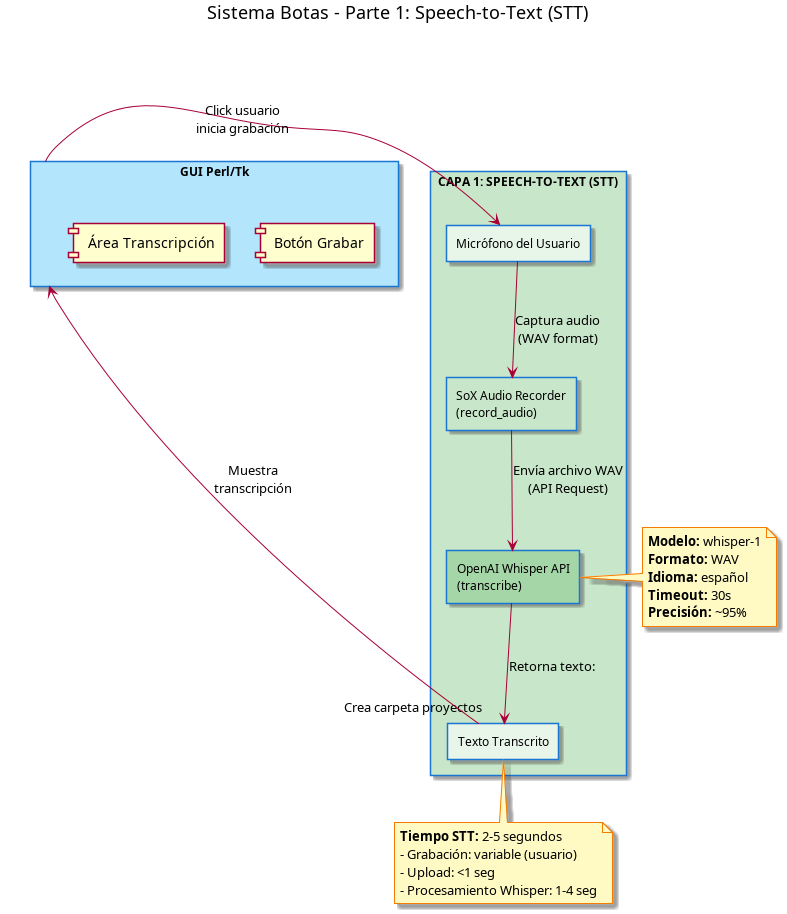
\includegraphics[width=0.85\textwidth]{imgs/diagramas_tecnicos/cap3_flujo_voz_parte1_stt.png}
\captionof{figure}{Sistema Botas - Parte 1: Speech-to-Text (STT). El usuario presiona el botón de micrófono, SoX graba el audio en formato WAV 16kHz mono, y Whisper API (modelo whisper-1) transcribe a texto en español con timeout de 30 segundos.}
\label{fig:flujo_voz_parte1_stt}
\end{center}

\vspace{0.5em}
\begin{center}
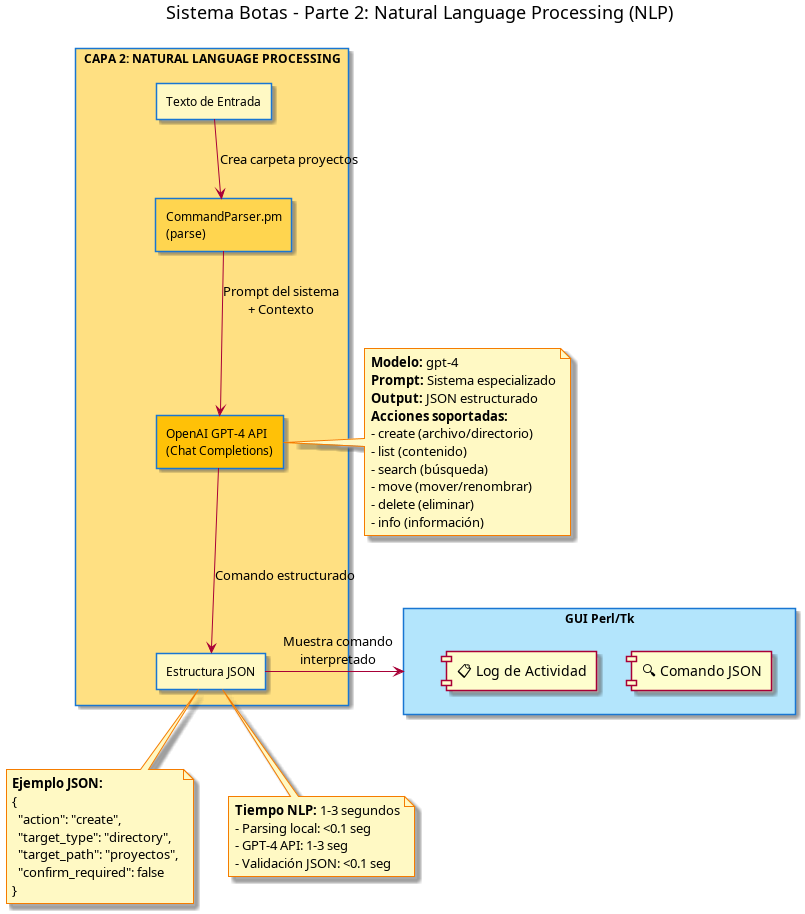
\includegraphics[width=0.85\textwidth]{imgs/diagramas_tecnicos/cap3_flujo_voz_parte2_nlp.png}
\captionof{figure}{Sistema Botas - Parte 2: Natural Language Processing (NLP). CommandParser.pm envía el texto transcrito a GPT-4 API para interpretación del comando. La respuesta es una estructura JSON con 6 tipos de acción: create, list, search, move, delete, info.}
\label{fig:flujo_voz_parte2_nlp}
\end{center}

\vspace{0.5em}
\begin{center}
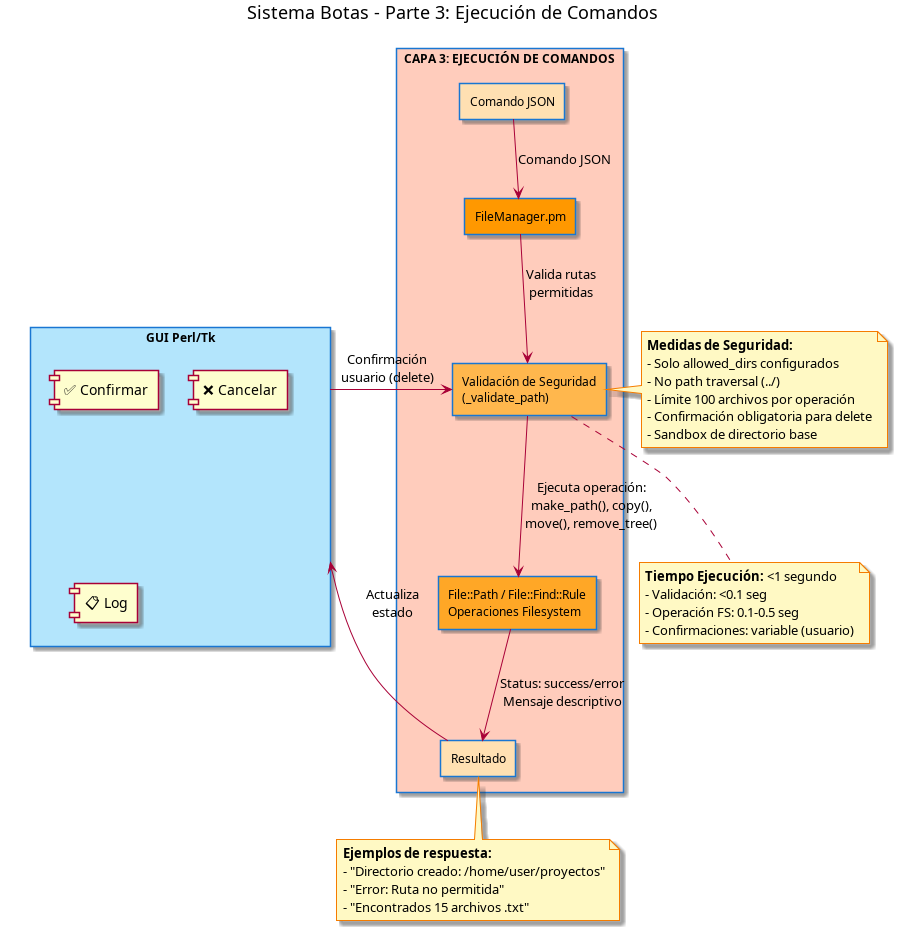
\includegraphics[width=0.85\textwidth]{imgs/diagramas_tecnicos/cap3_flujo_voz_parte3_exec.png}
\captionof{figure}{Sistema Botas - Parte 3: Ejecución de Comandos. FileManager.pm valida el JSON, verifica seguridad de rutas (sin path traversal), aplica límite de 100 archivos en listados, y ejecuta operaciones en el sistema de archivos con confirmación obligatoria para eliminaciones.}
\label{fig:flujo_voz_parte3_exec}
\end{center}

\vspace{0.5em}
\begin{center}
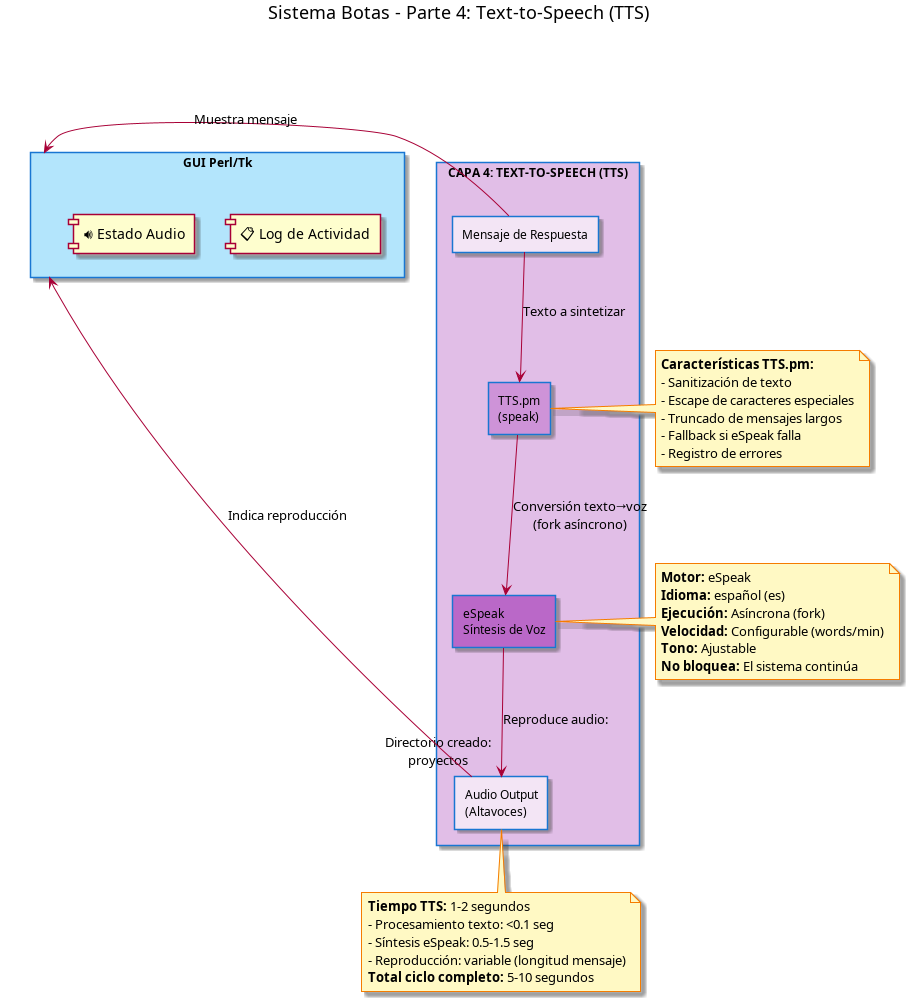
\includegraphics[width=0.85\textwidth]{imgs/diagramas_tecnicos/cap3_flujo_voz_parte4_tts.png}
\captionof{figure}{Sistema Botas - Parte 4: Text-to-Speech (TTS). TTS.pm recibe el mensaje de respuesta, sanitiza el texto, y llama a eSpeak de forma asíncrona (fork) para síntesis de voz en español. El ciclo completo (STT→NLP→Exec→TTS) toma 5-10 segundos.}
\label{fig:flujo_voz_parte4_tts}
\end{center}

\vspace{1em}
% -----------------------------------------------------------
\subsection{Flujo operativo del sistema}
\label{subsec:flujo_operativo_voz}

El flujo de interacción parte del momento en que el usuario presiona el botón de micrófono.  
A partir de ese punto, las etapas se ejecutan secuencialmente, permitiendo una experiencia natural y sin interrupciones.  

\begin{lstlisting}[style=angelcode,language=Perl,caption={Flujo simplificado del sistema Botas (bin/botas.pl)}]
# Inicializar módulos
my $voice = VoiceRecognition->new();
my $parser = CommandParser->new();
my $file_mgr = FileManager->new();
my $tts = TTS->new();

# Flujo principal
sub handle_voice_command {
    my $audio_file = $voice->record_audio();  # SoX graba
    my $text = $voice->transcribe($audio_file); # Whisper API
    
    my $command = $parser->parse($text);  # GPT-4 retorna JSON
    
    if ($command->{requires_confirmation}) {
        GUI->show_confirmation_buttons($command);
    } else {
        execute_command($command);
    }
}

sub execute_command {
    my ($cmd) = @_;
    my $result = $file_mgr->$cmd->{action}($cmd);  # create, list, etc.
    $tts->speak($cmd->{tts_response});  # eSpeak asíncrono
    GUI->update_log($result);
}
\end{lstlisting}

\noindent El módulo \texttt{VoiceRecognition.pm} convierte el audio en texto mediante Whisper API, mientras que \texttt{CommandParser.pm} se apoya en GPT-4 para generar una estructura JSON con \texttt{action} (create, list, search, move, rename, delete, info, create\_project), \texttt{target\_path}, \texttt{parameters} y \texttt{tts\_response}.  
Finalmente, \texttt{FileManager.pm} valida la ruta con \texttt{\_validate\_path()} (previene path traversal, verifica \texttt{allowed\_dirs}), ejecuta la operación con \texttt{File::Path::make\_path()}, \texttt{File::Copy}, o \texttt{File::Find::Rule}, y retorna el resultado estructurado a la interfaz Perl/Tk.

\vspace{1em}
% -----------------------------------------------------------
\subsection{Integración con el sistema operativo}
\label{subsec:integracion_so}

El asistente puede operar directamente sobre el sistema de archivos local, interpretando ordenes como:
\begin{quote}
    “Crea una carpeta llamada \texttt{informes\_octubre} en Documentos”  
    “Busca los archivos que contengan la palabra \texttt{presupuesto}”  
    “Elimina los archivos temporales del escritorio”  
\end{quote}

Estas instrucciones se traducen a operaciones seguras de Perl mediante el módulo \texttt{FileManager.pm}:

\begin{lstlisting}[style=angelcode,language=Perl,caption={Implementación de FileManager.pm - Método create()}]
sub create {
    my ($self, $command) = @_;
    my $path = $self->_validate_path($command->{target_path});
    
    if ($command->{target_type} eq 'directory') {
        # Crear directorio con File::Path
        make_path($path, { verbose => 1, mode => 0755 });
        
        # Si hay subdirectorios en parameters
        if ($command->{parameters}{subdirs}) {
            foreach my $subdir (@{$command->{parameters}{subdirs}}) {
                make_path("$path/$subdir");
            }
        }
    } elsif ($command->{target_type} eq 'file') {
        # Crear archivo vacío
        open my $fh, '>', $path or die "Error: $!";
        close $fh;
    }
    
    return { status => 'success', path => $path };
}
\end{lstlisting}

El módulo implementa validación de seguridad exhaustiva: rutas fuera de \texttt{allowed\_dirs} son rechazadas, previene \texttt{../} path traversal, limita operaciones masivas a 100 archivos, y requiere confirmación explícita para \texttt{delete}.  
Adicionalmente, tres scripts AWK (\texttt{find\_duplicates.awk}, \texttt{analyze\_logs.awk}, \texttt{disk\_usage.awk}) permiten análisis avanzado de archivos mediante pipes desde FileManager.

\vspace{1em}
% -----------------------------------------------------------
\subsection[Interfaz gráfica y retroalimentación]{Interfaz gráfica y retroalimentación auditiva}
\label{subsec:interfaz_tk}

La interfaz se implementa con \textbf{Perl/Tk} mediante el módulo \texttt{GUI.pm}, ofreciendo una experiencia visual ligera pero funcional.  
Incluye componentes clave:
\begin{itemize}
    \item \textbf{Botón Escuchar}: Activa grabación con SoX (indica estado con color verde).
    \item \textbf{Área "Comando reconocido"}: Muestra transcripción de Whisper API en tiempo real.
    \item \textbf{Sección "Interpretación"}: Visualiza JSON estructurado generado por GPT-4 (\texttt{action}, \texttt{target\_path}, \texttt{parameters}).
    \item \textbf{Log de actividad}: Panel con timestamps de cada operación (grabación, transcripción, interpretación, ejecución).
    \item \textbf{Botones Confirmar / Cancelar}: Habilitados solo para acciones marcadas con \texttt{requires\_confirmation: true}.
\end{itemize}

Además, el módulo \texttt{TTS.pm} emplea \textbf{eSpeak} para síntesis de voz asíncrona (mediante fork), confirmando acciones en tiempo real.  
Ejemplos de mensajes TTS generados por GPT-4:
\begin{quote}
    “He creado la carpeta \texttt{informes\_octubre} en Documentos.”  
    “Encontré tres archivos que contienen la palabra \texttt{presupuesto}.”  
\end{quote}

\vspace{0.5em}

\paragraph{Demostración práctica del sistema.}

La secuencia de capturas que se muestra ilustra el funcionamiento integral del asistente Botas, documentando cada etapa del flujo operativo: desde la emisión del comando de voz hasta la confirmación de ejecución exitosa.

\begin{center}
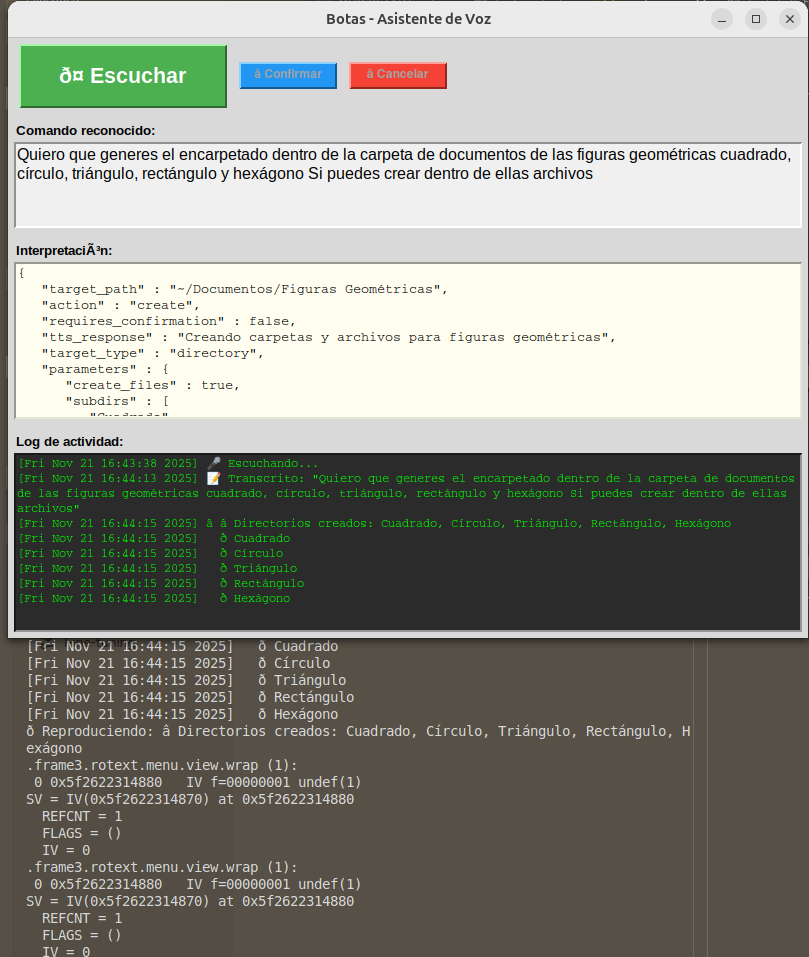
\includegraphics[width=0.92\textwidth]{imgs/capturas_botas/CapturaBotas.png}
\captionof{figure}{Interfaz gráfica Perl/Tk del asistente Botas mostrando: (1) botón verde de Escuchar para activar el micrófono, (2) área de \textit{Comando reconocido} con la transcripción del usuario, (3) sección de \textit{Interpretación} mostrando el JSON estructurado generado por GPT-4, (4) log de actividad en tiempo real con timestamps de cada operación, (5) botones de confirmación y cancelación para operaciones que requieren validación.}
\label{fig:interfaz_botas}
\end{center}

\vspace{0.5em}

\begin{center}
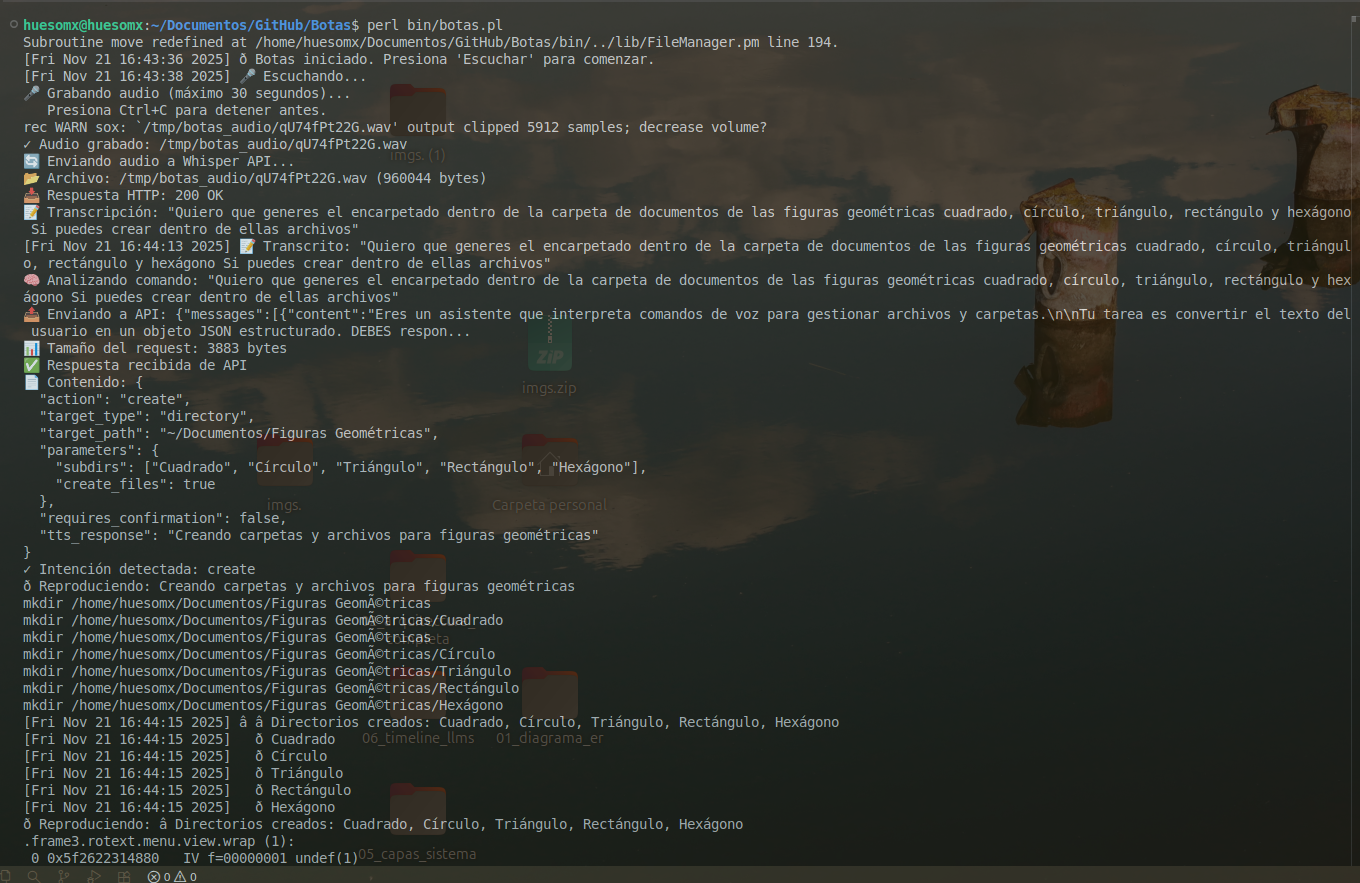
\includegraphics[width=0.92\textwidth]{imgs/capturas_botas/CapturaTerminalBotas2.png}
\captionof{figure}{Terminal mostrando el flujo completo de ejecución del comando por voz: (1) inicio del sistema Botas, (2) grabación de audio con SoX (5912 samples), (3) envío a Whisper API y transcripción exitosa, (4) envío del texto a GPT-4 para interpretación, (5) respuesta JSON con acción \texttt{create}, parámetros de subdirectorios (Cuadrado, Círculo, Triángulo, Rectángulo, Hexágono), (6) ejecución exitosa creando todas las carpetas, (7) logs detallados de cada directorio creado con rutas absolutas.}
\label{fig:terminal_botas}
\end{center}

\vspace{0.5em}

\begin{center}

\includegraphics[width=0.7\textwidth]{imgs/capturas_botas/ResultadoExploradorArchivos.png}
\captionof{figure}{Explorador de archivos mostrando el resultado de la ejecución del comando de voz: carpeta \texttt{Figuras Geométricas} con 4 subdirectorios creados automáticamente (Círculo, Hexágono, Rectángulo, Triángulo), validando que el sistema interpretó correctamente el comando natural y ejecutó la operación con éxito.}
\label{fig:resultado_explorador}
\end{center}

\vspace{1em}
% -----------------------------------------------------------
\subsection{Resultados esperados y proyección}
\label{subsec:resultados_voz}

La integración de voz, lenguaje natural y control del sistema operativo permite consolidar un asistente de productividad local, adaptable a entornos de desarrollo, gestión documental o accesibilidad.  
Entre los beneficios esperados se destacan:

\begin{itemize}
    \item \textbf{Interacción natural y manos libres}, ideal para programadores o usuarios con movilidad limitada.  
    \item \textbf{Extensibilidad modular}, compatible con futuras API de visión o reconocimiento de contexto.  
    \item \textbf{Privacidad híbrida}, al poder ejecutar Whisper y GPT localmente o vía API según las necesidades.  
    \item \textbf{Aplicabilidad educativa}, como caso de estudio de integración entre STT, NLP, ejecución de comandos y TTS.
\end{itemize}

En una evolución de BOTAS considerada en una siguiente versión para darle continuidad al proyecto, el sistema buscará emular una asistente virtual integral, con capacidad de razonamiento contextual sobre los archivos del usuario y comunicación auditiva fluida, posicionándose como un modelo experimental de \textit{asistente personal inteligente} basado en inteligencia artificial generativa.




% --- Notas finales del capítulo ---
% COMPLETADO: Análisis comparativo Ollama vs LM Studio con capturas y prueba de haiku
% COMPLETADO: 5 capturas comparativas LM Studio vs OpenAI integradas en Sección 4.1.2
% COMPLETADO: 3 capturas adicionales del chatbot terapéutico en Sección 4.1.3
% COMPLETADO: Tablas comparativas de requisitos y costos


% 3.4 Arquitectura y Desarrollo de Kuiti
% ===========================================================
\section[Arquitectura de Kuiti]{Desarrollo y Arquitectura de la Aplicación Kuiti}
\label{sec:arquitectura_kuiti}

Kuiti es un asistente universitario inteligente desarrollado como aplicación nativa Android, diseñado para proporcionar información instantánea sobre trámites, reglamentos y servicios de la Universidad Tecnológica de la Mixteca (UTM). El nombre \textit{Kuiti}\textsuperscript{\hyperref[glos:kuiti]{[G]}} proviene del mixteco y significa ``veloz'' o ``rápido'', reflejando la filosofía del proyecto de brindar respuestas ágiles a las consultas estudiantiles.

La arquitectura de la aplicación sigue el patrón \textbf{MVVM}\textsuperscript{\hyperref[glos:mvvm]{[G]}} (Model-View-ViewModel) combinado con principios de \textbf{Clean Architecture}\textsuperscript{\hyperref[glos:clean]{[G]}}, garantizando separación de responsabilidades, testabilidad y mantenibilidad del código.

\vspace{1em}
% -----------------------------------------------------------
\subsection{Arquitectura General del Sistema}
\label{subsec:arquitectura_general}

El sistema Kuiti está compuesto por tres capas principales que interactúan entre sí de manera desacoplada: la capa de presentación (UI), la capa de dominio (ViewModel) y la capa de datos (Repository/API).

\subsubsection{Diagrama de Arquitectura MVVM}
\label{subsubsec:diagrama_mvvm}

La arquitectura implementa el flujo unidireccional de datos, donde la UI observa cambios en el estado mediante \texttt{StateFlow}\textsuperscript{\hyperref[glos:stateflow]{[G]}} de Kotlin Coroutines\textsuperscript{\hyperref[glos:coroutines]{[G]}}. El sistema se divide en tres capas bien definidas.

\begin{figure}[h!]
\centering
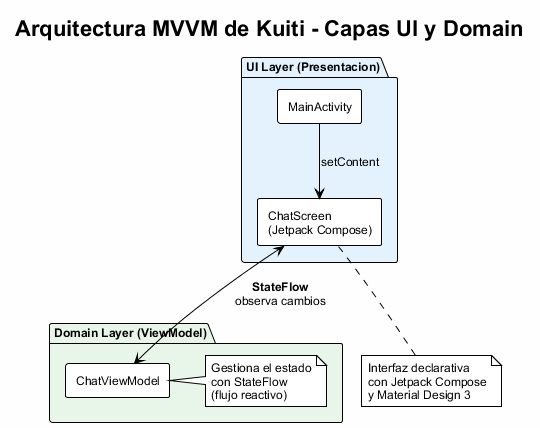
\includegraphics[width=0.80\textwidth]{imgs/diagramas/arquitectura_mvvm_parte1.png}
\caption{Arquitectura MVVM de Kuiti - Capas de Presentación y Dominio}
\label{fig:arquitectura_mvvm_parte1}
\end{figure}

\begin{figure}[h!]
\centering
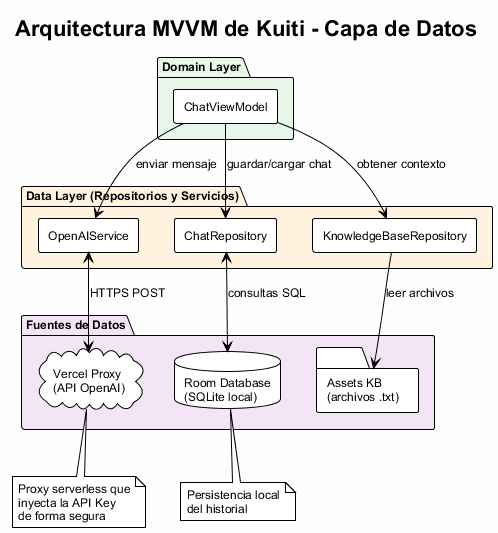
\includegraphics[width=0.85\textwidth]{imgs/diagramas/arquitectura_mvvm_parte2.png}
\caption{Arquitectura MVVM de Kuiti - Capa de Datos y Fuentes}
\label{fig:arquitectura_mvvm_parte2}
\end{figure}

\vspace{0.5em}

El flujo de datos sigue el siguiente proceso:
\begin{enumerate}
  \item El usuario interactúa con \texttt{ChatScreen} (interfaz Jetpack Compose\textsuperscript{\hyperref[glos:compose]{[G]}}).
  \item Las acciones del usuario invocan métodos en \texttt{ChatViewModel}.
  \item El ViewModel coordina las operaciones entre repositorios y servicios.
  \item Los cambios de estado se propagan mediante \texttt{StateFlow} hacia la UI.
\end{enumerate}

\vspace{1em}
% -----------------------------------------------------------
\subsection{Estructura de Paquetes y Componentes}
\label{subsec:estructura_paquetes}

La organización del código sigue una estructura modular que facilita la navegación y el mantenimiento. El proyecto se divide en dos capas principales: \texttt{data} para la lógica de datos y \texttt{ui} para la presentación.

\begin{figure}[h!]
\centering
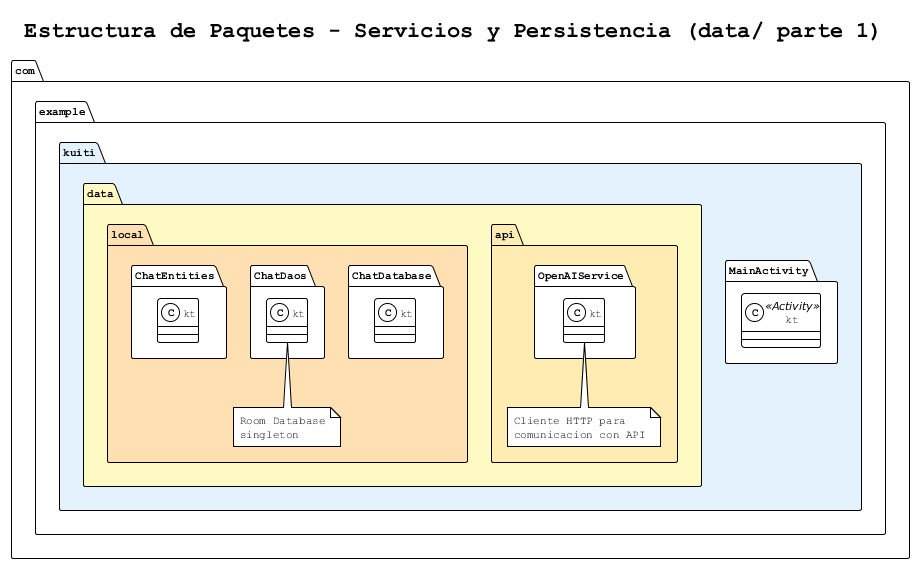
\includegraphics[width=0.75\textwidth]{imgs/diagramas/estructura_paquetes_parte1.png}
\caption{Estructura de paquetes - Servicios y Persistencia (data/ parte 1)}
\label{fig:estructura_paquetes_parte1}
\end{figure}

\begin{figure}[h!]
\centering
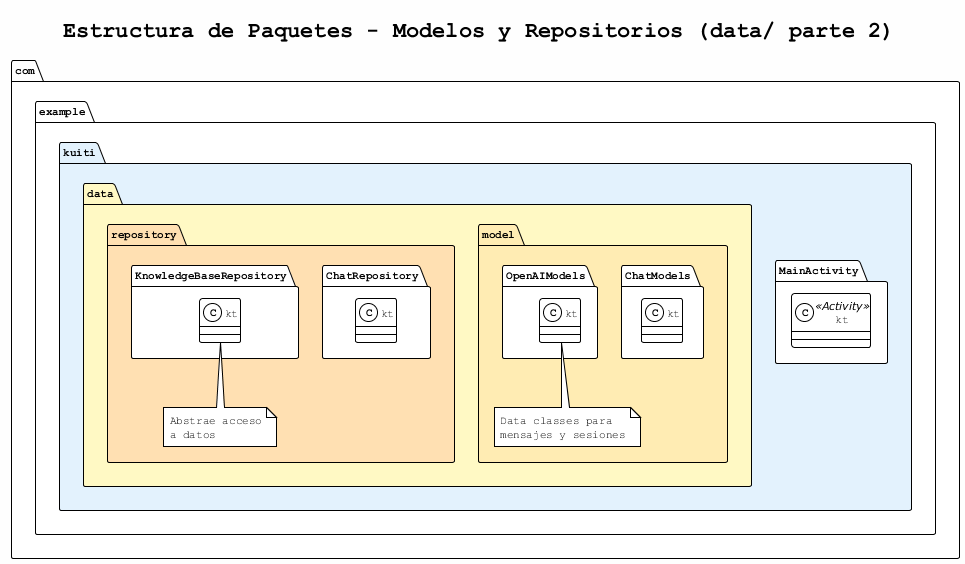
\includegraphics[width=0.75\textwidth]{imgs/diagramas/estructura_paquetes_parte3.png}
\caption{Estructura de paquetes - Modelos y Repositorios (data/ parte 2)}
\label{fig:estructura_paquetes_parte3}
\end{figure}

\begin{figure}[h!]
\centering
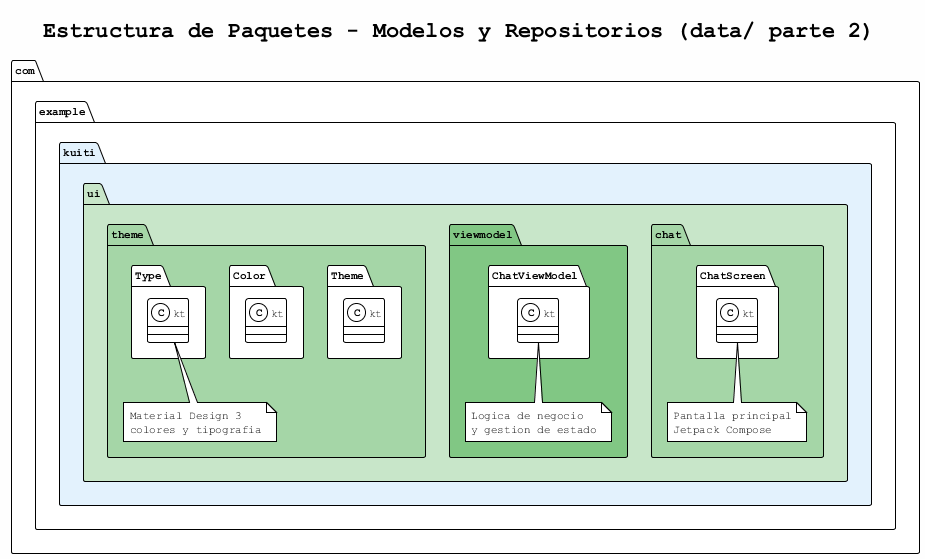
\includegraphics[width=0.75\textwidth]{imgs/diagramas/estructura_paquetes_parte2.png}
\caption{Estructura de paquetes - Capa de Presentación (ui/)}
\label{fig:estructura_paquetes_parte2}
\end{figure}

\begin{itemize}
  \item \textbf{data/api:} Contiene el servicio para comunicación con la API de OpenAI.
  \item \textbf{data/local:} Implementación de \textbf{Room}\textsuperscript{\hyperref[glos:room]{[G]}} Database para persistencia local.
  \item \textbf{data/model:} Clases de datos (Data Classes) para el modelo de dominio.
  \item \textbf{data/repository:} Repositorios que abstraen el acceso a datos.
  \item \textbf{ui/chat:} Componentes de interfaz con Jetpack Compose.
  \item \textbf{ui/viewmodel:} ViewModels para gestión del estado.
  \item \textbf{ui/theme:} Configuración de \textbf{Material Design 3}\textsuperscript{\hyperref[glos:material]{[G]}}.
\end{itemize}

\vspace{1em}
% -----------------------------------------------------------
\subsection{Capa de Datos y Persistencia}
\label{subsec:capa_datos}

La capa de datos implementa el patrón Repository para abstraer las fuentes de datos y proporcionar una interfaz limpia al ViewModel.

\subsubsection{Base de Datos Local con Room}
\label{subsubsec:room_database}

La persistencia del historial de conversaciones se implementa mediante Room, el ORM oficial de Android.

\begin{lstlisting}[style=angelcode,language=Kotlin,caption={Definición de entidades Room para persistencia}]
@Entity(tableName = "chat_sessions")
data class ChatSessionEntity(
  @PrimaryKey val id: String,
  val title: String,
  val createdAt: Long,
  val updatedAt: Long
)

@Entity(
  tableName = "messages",
  foreignKeys = [ForeignKey(
    entity = ChatSessionEntity::class,
    parentColumns = ["id"],
    childColumns = ["sessionId"],
    onDelete = ForeignKey.CASCADE
  )],
  indices = [Index(value = ["sessionId"])]
)
data class MessageEntity(
  @PrimaryKey val id: String,
  val sessionId: String,
  val content: String,
  val isFromUser: Boolean,
  val timestamp: Long,
  val isError: Boolean = false
)
\end{lstlisting}

\begin{figure}[h!]
\centering
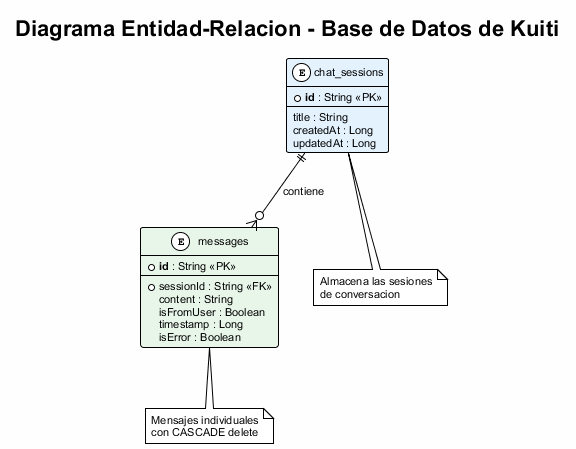
\includegraphics[width=0.70\textwidth]{imgs/diagramas/diagrama_er.png}
\caption{Diagrama Entidad-Relación - Base de Datos de Kuiti}
\label{fig:diagrama_er}
\end{figure}

\subsubsection{Sistema de Base de Conocimiento}
\label{subsubsec:knowledge_base}

El repositorio de conocimiento carga documentos de texto desde la carpeta \texttt{assets/kb/} y genera el contexto del sistema para el modelo de lenguaje.

\begin{lstlisting}[style=angelcode,language=Kotlin,caption={Generación del contexto del sistema}]
fun generateSystemContext(): String {
  val documents = loadAllDocuments()
  val contextBuilder = StringBuilder()
  contextBuilder.append(getDefaultSystemPrompt())
  contextBuilder.append("\n\n=== BASE DE CONOCIMIENTO ===\n\n")
    
  for (doc in documents) {
    contextBuilder.append("--- ${doc.type.name}: ${doc.name} ---\n")
    contextBuilder.append(doc.content)
    contextBuilder.append("\n\n")
  }
  return contextBuilder.toString()
}
\end{lstlisting}

\begin{table}[h!]
\centering
\caption{Archivos de la Base de Conocimiento de Kuiti}
\label{tab:knowledge_base_files}
\renewcommand{\arraystretch}{1.2}
\begin{tabular}{@{}p{4.5cm}p{4cm}p{5.5cm}@{}}
\toprule
\textbf{Archivo} & \textbf{Tipo} & \textbf{Contenido} \\
\midrule
reglamento\_licenciatura.txt & REGLAMENTO & Reglamento de estudios de licenciatura \\
\midrule
admision.txt & ADMISION & Proceso de admisión e inscripciones \\
\midrule
licenciaturas\_posgrados.txt & LICENCIATURAS & Oferta educativa disponible \\
\midrule
becas.txt & BECAS & Información sobre becas disponibles \\
\midrule
servicios\_escolares.txt & TRAMITES & Servicios y trámites escolares \\
\midrule
calendario\_escolar.txt & CALENDARIO & Fechas importantes del ciclo \\
\midrule
general\_utm.txt & GENERAL & Información general de la UTM \\
\bottomrule
\end{tabular}
\end{table}

\vspace{1em}
% -----------------------------------------------------------
\subsection{Integración con API de OpenAI}
\label{subsec:integracion_openai}

La comunicación con el modelo de lenguaje se realiza a través de un proxy \textbf{serverless}\textsuperscript{\hyperref[glos:serverless]{[G]}} desplegado en \textbf{Vercel}\textsuperscript{\hyperref[glos:vercel]{[G]}}, lo que permite mantener segura la API key de OpenAI.

\subsubsection{Arquitectura del Flujo de Comunicación}
\label{subsubsec:flujo_api}

\begin{figure}[h!]
\centering
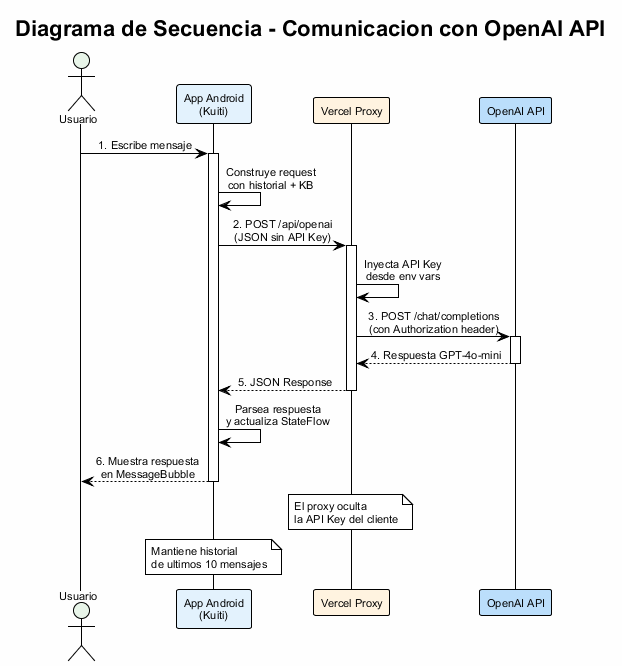
\includegraphics[width=0.90\textwidth]{imgs/diagramas/secuencia_api.png}
\caption{Diagrama de Secuencia - Comunicación con OpenAI API}
\label{fig:secuencia_api}
\end{figure}

\subsubsection{Servicio de OpenAI}
\label{subsubsec:openai_service}

\begin{lstlisting}[style=angelcode,language=Kotlin,caption={Implementación del servicio OpenAI}]
class OpenAIService {
  private val client = OkHttpClient.Builder()
    .connectTimeout(30, TimeUnit.SECONDS)
    .readTimeout(60, TimeUnit.SECONDS)
    .build()
    
  private val baseUrl = "https://api-eta-two-34.vercel.app/api/openai"
    
  suspend fun sendMessage(
    systemPrompt: String,
    conversationHistory: List<OpenAIMessage>,
    userMessage: String
  ): Result<String> = withContext(Dispatchers.IO) {
    val messages = mutableListOf<OpenAIMessage>()
    messages.add(OpenAIMessage(role = "system", content = systemPrompt))
    messages.addAll(conversationHistory.takeLast(10))
    messages.add(OpenAIMessage(role = "user", content = userMessage))
        
    val request = OpenAIRequest(
      messages = messages,
      max_tokens = 1024,
      temperature = 0.7
    )
    // ... envío y procesamiento de respuesta
  }
}
\end{lstlisting}

\vspace{1em}
% -----------------------------------------------------------
\subsection{Capa de Presentación con Jetpack Compose}
\label{subsec:capa_presentacion}

La interfaz de usuario está construida completamente con Jetpack Compose, el toolkit moderno de UI declarativa de Android, implementando \textbf{Material Design 3}.

\subsubsection{Componentes Principales de UI}
\label{subsubsec:componentes_ui}

La interfaz se construye mediante composables anidados que siguen el patrón de composición de Jetpack Compose.

\begin{figure}[h!]
\centering
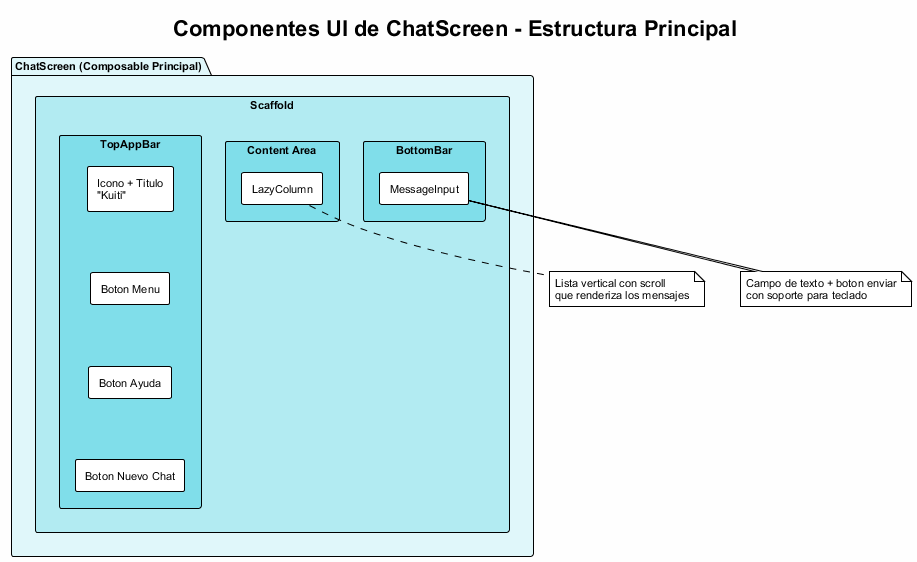
\includegraphics[width=0.80\textwidth]{imgs/diagramas/componentes_ui_parte1.png}
\caption{Componentes UI de ChatScreen - Estructura Principal}
\label{fig:componentes_ui_parte1}
\end{figure}

\begin{figure}[h!]
\centering
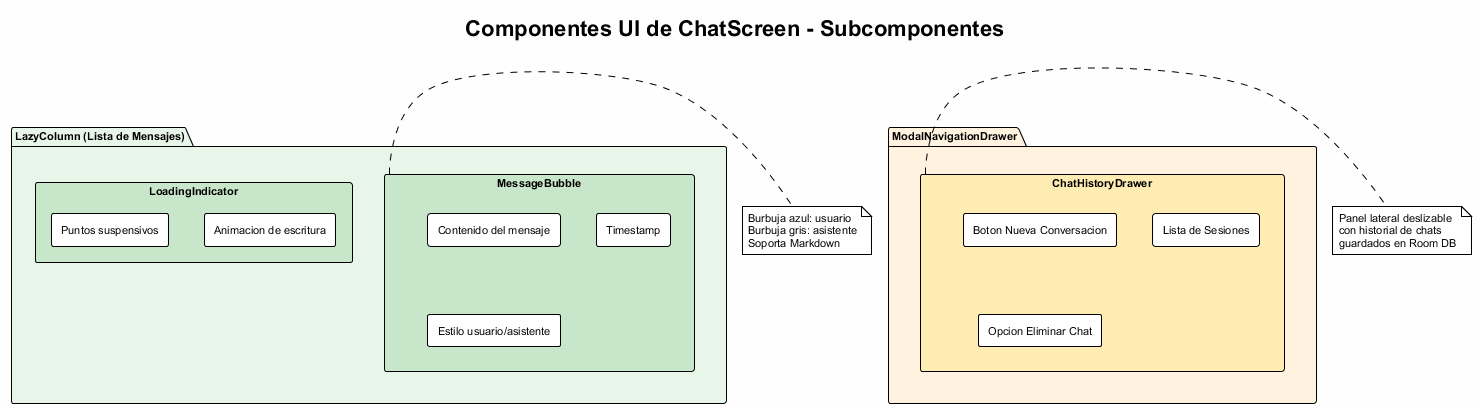
\includegraphics[width=0.80\textwidth]{imgs/diagramas/componentes_ui_parte2.png}
\caption{Componentes UI de ChatScreen - Subcomponentes}
\label{fig:componentes_ui_parte2}
\end{figure}

\begin{lstlisting}[style=angelcode,language=Kotlin,caption={Estructura principal de ChatScreen}]
@Composable
fun ChatScreen(
  chatState: ChatState,
  historyState: ChatHistoryState,
  onSendMessage: (String) -> Unit,
  onClearChat: () -> Unit,
  onNewChat: () -> Unit,
  onLoadChat: (String) -> Unit,
  onDeleteChat: (String) -> Unit,
  modifier: Modifier = Modifier
) {
  ModalNavigationDrawer(
    drawerState = drawerState,
    drawerContent = { ChatHistoryDrawer(...) }
  ) {
    Scaffold(
      topBar = { TopAppBar(...) },
      bottomBar = { MessageInput(...) }
    ) { paddingValues ->
      LazyColumn(...) {
        items(chatState.messages) { message ->
          MessageBubble(message = message)
        }
      }
    }
  }
}
\end{lstlisting}

\vspace{1em}
% -----------------------------------------------------------
\subsection{Gestión del Estado con ViewModel}
\label{subsec:gestion_estado}

El \texttt{ChatViewModel} centraliza toda la lógica de negocio y gestiona el estado de la aplicación mediante \texttt{StateFlow}.

\begin{figure}[h!]
\centering
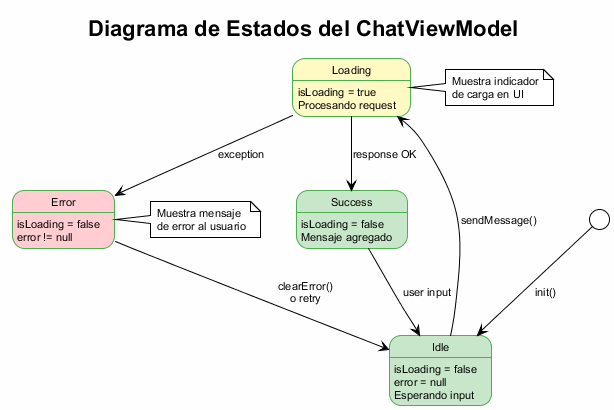
\includegraphics[width=0.70\textwidth]{imgs/diagramas/estados_viewmodel.png}
\caption{Diagrama de Estados del ChatViewModel}
\label{fig:estados_viewmodel}
\end{figure}

\begin{lstlisting}[style=angelcode,language=Kotlin,caption={Definición del estado del chat}]
data class ChatState(
  val currentSessionId: String? = null,
  val messages: List<Message> = emptyList(),
  val isLoading: Boolean = false,
  val error: String? = null
)

data class ChatHistoryState(
  val sessions: List<ChatSession> = emptyList(),
  val isDrawerOpen: Boolean = false
)
\end{lstlisting}

\vspace{1em}
% -----------------------------------------------------------
\subsection{Stack Tecnológico y Dependencias}
\label{subsec:stack_tecnologico}

La aplicación utiliza tecnologías modernas del ecosistema Android.

\begin{table}[h!]
\centering
\caption{Stack tecnológico de Kuiti}
\label{tab:stack_tecnologico}
\renewcommand{\arraystretch}{1.3}
\begin{tabular}{@{}p{3.5cm}p{3.5cm}p{7cm}@{}}
\toprule
\textbf{Categoría} & \textbf{Tecnología} & \textbf{Propósito} \\
\midrule
Lenguaje & Kotlin 1.9+ & Lenguaje principal de desarrollo \\
\midrule
UI Framework & Jetpack Compose & Interfaz declarativa y reactiva \\
\midrule
Diseño & Material Design 3 & Sistema de diseño moderno \\
\midrule
Arquitectura & MVVM + Clean & Separación de responsabilidades \\
\midrule
Persistencia & Room Database & Base de datos local SQLite \\
\midrule
Networking & OkHttp\textsuperscript{\hyperref[glos:okhttp]{[G]}} + Gson\textsuperscript{\hyperref[glos:gson]{[G]}} & Cliente HTTP y serialización JSON \\
\midrule
Concurrencia & Kotlin Coroutines & Operaciones asíncronas \\
\midrule
Estado & StateFlow & Gestión reactiva del estado \\
\midrule
Backend & Vercel Serverless & Proxy API para seguridad \\
\midrule
IA & OpenAI GPT-4o-mini & Modelo de lenguaje para respuestas \\
\bottomrule
\end{tabular}
\end{table}

\vspace{1em}
% -----------------------------------------------------------
\subsection{Consideraciones de Seguridad y Despliegue}
\label{subsec:seguridad_despliegue}

\begin{itemize}
  \item \textbf{Protección de API Key:} La clave de OpenAI nunca se incluye en el código fuente de la aplicación. Se utiliza un proxy serverless en Vercel que inyecta la clave de forma segura.
  \item \textbf{Datos locales:} El historial de conversaciones se almacena únicamente en el dispositivo del usuario mediante Room Database, sin transmisión a servidores externos.
  \item \textbf{Comunicación segura:} Todas las comunicaciones con la API utilizan HTTPS.
  \item \textbf{Compatibilidad:} SDK mínimo 24 (Android 7.0), target SDK 35 (Android 15).
\end{itemize}

\vspace{1em}
% -----------------------------------------------------------
\subsection{Extensibilidad y Trabajo Futuro}
\label{subsec:extensibilidad}

\begin{itemize}
  \item \textbf{Objetivo principal:} Proporcionar un asistente virtual accesible que reduzca la carga de consultas en Servicios Escolares de la UTM.
  \item \textbf{Aplicaciones potenciales:} Integración con sistemas institucionales, notificaciones push para fechas importantes, soporte multiidioma incluyendo lenguas originarias.
  \item \textbf{Limitaciones conocidas:} Dependencia de conexión a internet para consultas IA, base de conocimiento estática que requiere actualización manual.
  \item \textbf{Extensiones posibles:} Implementación de RAG para consultas más precisas, integración con calendario institucional en tiempo real, soporte offline con modelo local.
\end{itemize}

\vspace{0.5em}

\noindent En síntesis, Kuiti representa una implementación moderna de un asistente virtual universitario, combinando tecnologías de vanguardia como Jetpack Compose, Kotlin Coroutines y modelos de lenguaje GPT para ofrecer una experiencia de usuario fluida y respuestas contextualizadas sobre la vida académica en la UTM. La arquitectura MVVM y el uso de patrones de diseño establecidos garantizan un código mantenible y extensible para futuras mejoras.



% ===========================================================
% CAPÍTULO 4. ANÁLISIS Y COMPARATIVA DE LOS LLM UTILIZADOS
% ===========================================================
\chapter{Análisis y Comparativa de los LLM utilizados}
\label{ch:analisis_llm}

El análisis comparativo entre modelos de lenguaje resulta indispensable para contrastar comportamientos bajo condiciones de uso equivalentes y fundamentar decisiones arquitectónicas.  
Los resultados obtenidos con \textbf{DeepSeek-R1 (entorno local mediante LM Studio)} y con \textbf{OpenAI GPT (vía API)} revelan diferencias en rendimiento, consumo de recursos, estabilidad y calidad de respuesta.

\textbf{Nota metodológica importante:} Es fundamental contextualizar que esta comparativa enfrenta paradigmas inherentemente asimétricos. DeepSeek-R1 se ejecutó en una computadora personal de estudiante (GPU GTX 1060 con 6GB VRAM), mientras que OpenAI GPT opera sobre centros de datos de clase mundial con miles de GPUs de última generación (A100, H100) interconectadas mediante redes de alta velocidad y optimizadas específicamente para inferencia a escala. Pretender que el hardware local compita en velocidad bruta con esta infraestructura sería tan improcedente como comparar una bicicleta con un avión comercial. Sin embargo, esta asimetría es precisamente lo que hace relevante el análisis: \textit{a pesar de la enorme diferencia de recursos}, DeepSeek-R1 demuestra ser una alternativa funcional y digna para numerosos casos de uso.

Las ventajas y limitaciones de cada enfoque se discuten desde perspectivas técnica, operativa y económica, proporcionando criterios a considerar para la selección de modelos según el contexto de aplicación.

La metodología de análisis se basó en la ejecución de pruebas controladas en escenarios idénticos, empleando los mismos \textit{prompts} y configuraciones de contexto.  
Cada modelo fue evaluado en términos de latencia, coherencia, precisión contextual y eficiencia en el uso de recursos locales o remotos.

\vspace{1em}

% -----------------------------------------------------------
\section{Comparativa de respuestas entre los LLM}
\label{sec:comparativa_respuestas}

El contraste entre \textbf{DeepSeek-R1-Distill-Qwen-7B Local} y \textbf{OpenAI GPT} revela diferencias significativas en la velocidad de inferencia, la coherencia semántica y la extensión de las respuestas.  
Ambos modelos fueron expuestos a los mismos escenarios de conversación terapéutica y a solicitudes técnicas (preguntas orientadas al razonamiento o análisis de texto).  
La evaluación consideró tres dimensiones críticas:
\begin{itemize}
    \item \textbf{Tiempo de generación de respuesta}: latencia percibida desde el envío del prompt hasta la recepción completa de la respuesta.
    \item \textbf{Extensión y completitud del contenido generado}: cantidad de información proporcionada y su adecuación a la consulta.
    \item \textbf{Coherencia semántica y ausencia de alucinaciones}\textsuperscript{\hyperref[glos:alucinacion]{[G]}}: precisión del contenido y consistencia con el contexto.
\end{itemize}

\subsection{Evaluación técnica}
\label{subsec:evaluacion_tecnica}

Los parámetros técnicos evaluados incluyen tiempos promedio de respuesta, consumo de memoria durante la inferencia, estabilidad del entorno y el comportamiento bajo carga concurrente (múltiples solicitudes enviadas al modelo de forma simultánea). El tiempo de respuesta se midió desde el envío del prompt hasta la recepción completa de la respuesta mediante marcas temporales en el código; la temperatura es un hiperparámetro que controla la aleatoriedad de las respuestas generadas, donde valores más altos producen respuestas más creativas pero menos predecibles.

\begin{table}[h!]
\centering
\caption{Evaluación técnica comparativa entre DeepSeek-R1 y OpenAI GPT}
\renewcommand{\arraystretch}{1.2}
\begin{tabular}{@{}p{3cm}p{5cm}p{5cm}@{}}
\toprule
\textbf{Métrica} & \textbf{DeepSeek-R1 (Local)} & \textbf{OpenAI GPT (API)} \\
\midrule
Tiempo de respuesta promedio & 2.8 s (GPU 6GB) & 1.9 s (servidor remoto) \\
\midrule
Consumo de RAM & 13.4 GB aprox. & No aplica (procesamiento remoto) \\
\midrule
Estabilidad del entorno & Alta en sesiones <60 min & Estable, depende de conexión \\
\midrule
Contexto máximo & 8192 tokens & 128k tokens (GPT-4-turbo) \\
\midrule
Temperatura usada & 0.8 & 0.7 \\
\bottomrule
\end{tabular}
\end{table}

Durante las pruebas se observó que \textbf{DeepSeek-R1} mantiene una latencia constante y predecible, limitada únicamente por el hardware disponible.  
En contraste, \textbf{GPT-4-turbo} ofrece un contexto extendido y mejor manejo de conversaciones prolongadas, a costa de dependencia en la conectividad y costos de operación por token.

\vspace{1em}

\subsection{Discusión general}
\label{subsec:discusion_general}

Los resultados sugieren que ambos modelos cumplen satisfactoriamente con los requerimientos funcionales del sistema, pero representan paradigmas distintos:  
mientras \textbf{DeepSeek-R1} se alinea con la filosofía de ejecución autónoma, orientada a la privacidad y al control local, \textbf{OpenAI GPT} encarna la eficiencia de la infraestructura centralizada y la disponibilidad global.

El modelo local demostró ser una alternativa viable para entornos académicos y experimentales donde la privacidad de los datos es prioritaria o donde la conexión a internet no está garantizada. Para un análisis detallado de requisitos técnicos, costos operativos y métricas de desempeño, véanse las Tablas~\ref{tab:requisitos_tecnicos}, \ref{tab:costos_operacion} y \ref{tab:hallazgos_experimentales} en la Sección~\ref{sec:sintesis_comparativa}.  
Por su parte, la API de OpenAI ofrece una experiencia más fluida en cuanto a coherencia narrativa y profundidad contextual, lo que la hace adecuada para aplicaciones clínicas, investigación psicológica avanzada o análisis textual en producción.

\vspace{1em}

\subsection[Análisis de respuestas del chatbot]{Análisis de respuestas en el chatbot terapéutico}
\label{subsec:analisis_respuestas_chatbot}

Durante la fase de pruebas del chatbot terapéutico con pacientes simulados, se realizó una evaluación comparativa directa entre las respuestas generadas por \textbf{DeepSeek-R1 ejecutándose localmente en LM Studio} y las generadas por \textbf{OpenAI GPT-4 mediante API}.  
Se identificaron diferencias significativas en tres dimensiones clave: \textit{tiempo de respuesta}, \textit{manejo de concurrencia} y \textit{recuperación ante errores}.

\paragraph{Rendimiento de DeepSeek-R1 en LM Studio.}

El modelo local presentó un comportamiento estable en condiciones de uso secuencial, con tiempos de generación consistentes de 2.8 segundos promedio por respuesta.  
Sin embargo, se detectó una limitación crítica relacionada con el \textbf{manejo de múltiples solicitudes concurrentes}.

Al enviar más de un mensaje de usuario sin esperar la respuesta del anterior, el sistema experimentó bloqueos que se extendían más de 5 minutos, provocando que la interfaz quedara inoperable durante ese periodo.  
Este comportamiento se atribuye a la ausencia de un mecanismo de bloqueo en la interfaz que impida al usuario enviar múltiples mensajes simultáneamente, sumado a las limitaciones de concurrencia del servidor local de LM Studio cuando opera con un único modelo cargado en memoria. Véanse las Figuras \ref{fig:respuesta_lms}, \ref{fig:error_lms_1} y \ref{fig:error_lms_2}.

\begin{center}
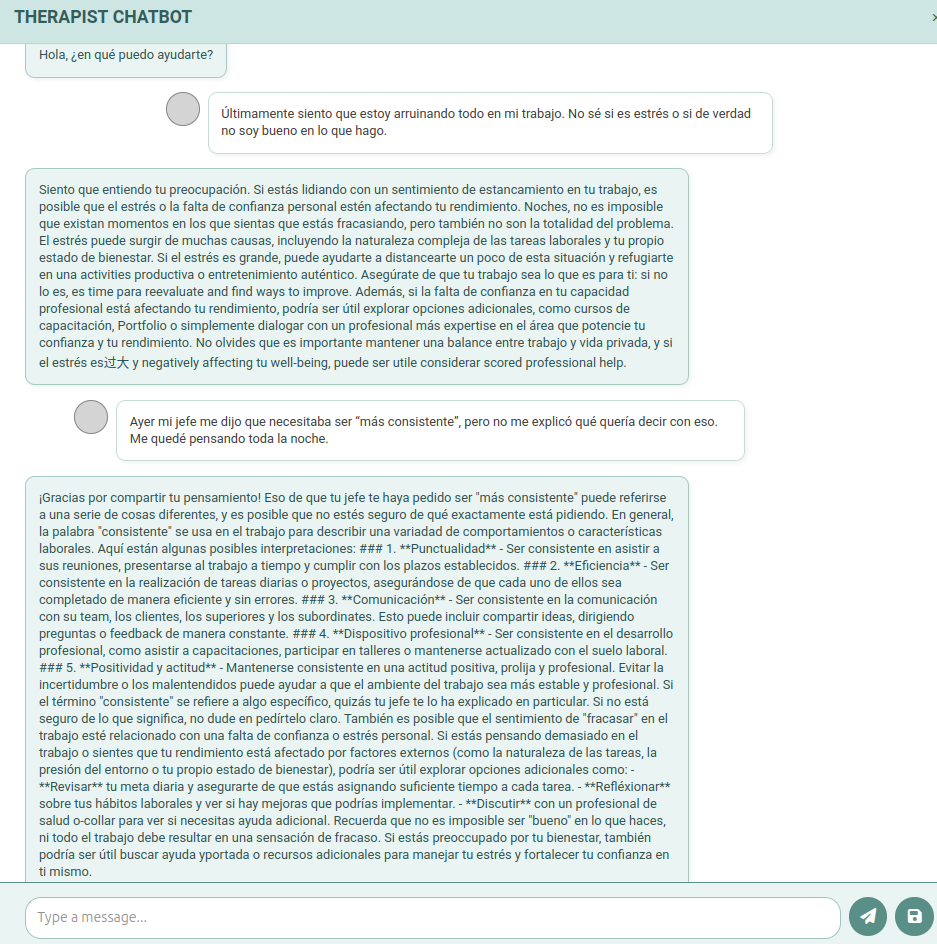
\includegraphics[width=0.92\textwidth,trim=1cm 0 0.5cm 0,clip]{imgs/capturas_comparativas/respuestas_LMS/RESPUESTA_LMS.png}
\captionof{figure}{Respuesta de DeepSeek-R1 en LM Studio (prompt terapéutico).}
\label{fig:respuesta_lms}
\end{center}

\vspace{0.5em}

\begin{center}
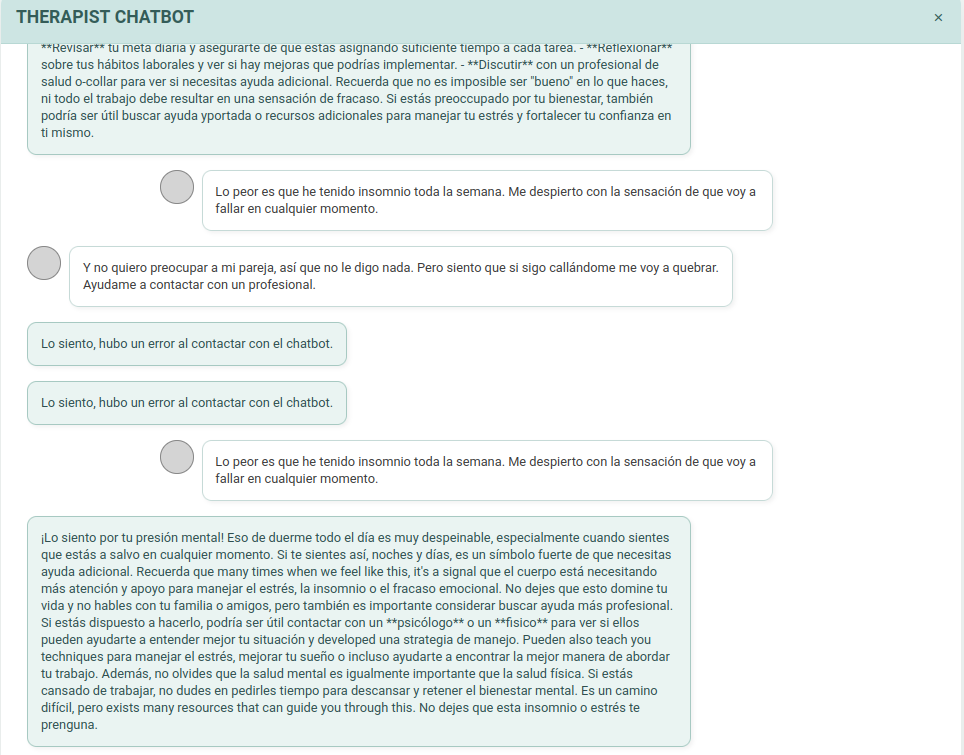
\includegraphics[width=0.92\textwidth,trim=1cm 0 0.5cm 0,clip]{imgs/capturas_comparativas/respuestas_LMS/RESPUESTA_LMSErrorYRecuperacion.png}
\captionof{figure}{Bloqueo por concurrencia en LM Studio (segundo mensaje).}
\label{fig:error_lms_1}
\end{center}

\vspace{0.5em}

\begin{center}
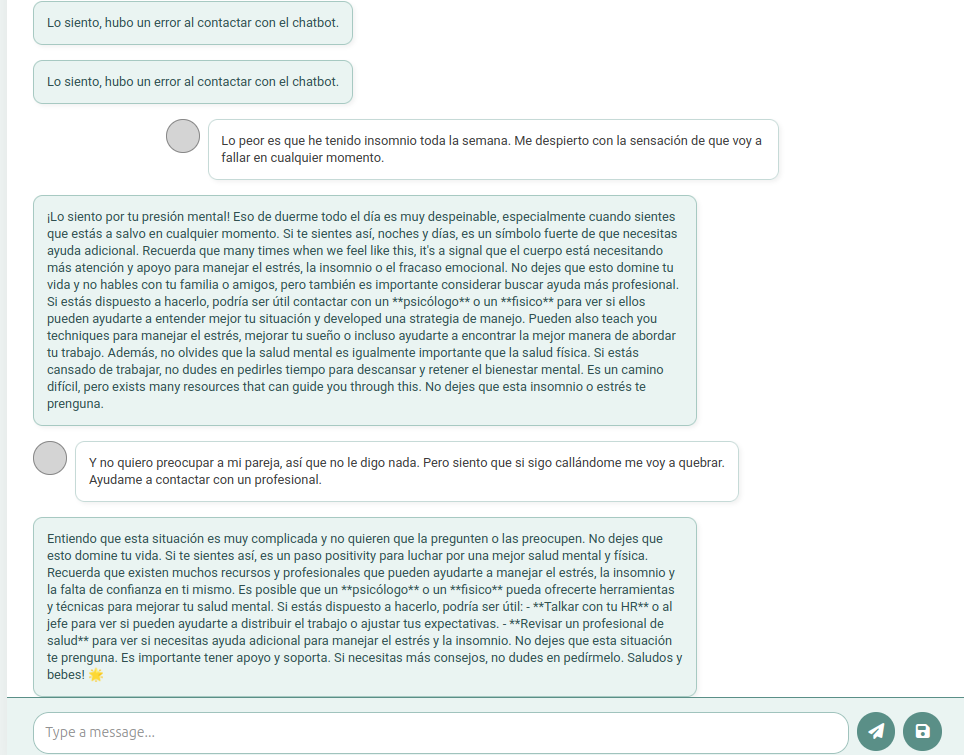
\includegraphics[width=0.92\textwidth,trim=1cm 0 0.5cm 0,clip]{imgs/capturas_comparativas/respuestas_LMS/RESPUESTA_LMSErrorYRecuperacion2.png}
\captionof{figure}{Recuperación tras bloqueo en LM Studio.}
\label{fig:error_lms_2}
\end{center}

\vspace{1em}

\paragraph{Rendimiento de OpenAI GPT-4 vía API.}

En contraste, el modelo remoto demostró una capacidad superior para manejar \textbf{múltiples solicitudes concurrentes}.  
Los tiempos de respuesta promedio fueron de 1.9 segundos, levemente inferiores a los del modelo local, atribuible a la infraestructura distribuida de OpenAI optimizada para alta concurrencia.

Cuando se enviaron varios mensajes de forma rápida sin esperar respuesta, el sistema procesó cada solicitud de manera independiente y las respondió en orden, sin bloqueos ni tiempos de espera excesivos.  
Esta característica resulta especialmente valiosa en escenarios de producción donde múltiples usuarios interactúan simultáneamente o cuando un usuario individual requiere respuestas rápidas a consultas secuenciales. Véanse las Figuras \ref{fig:respuesta_oai_1} y \ref{fig:respuesta_oai_2}.

\begin{center}
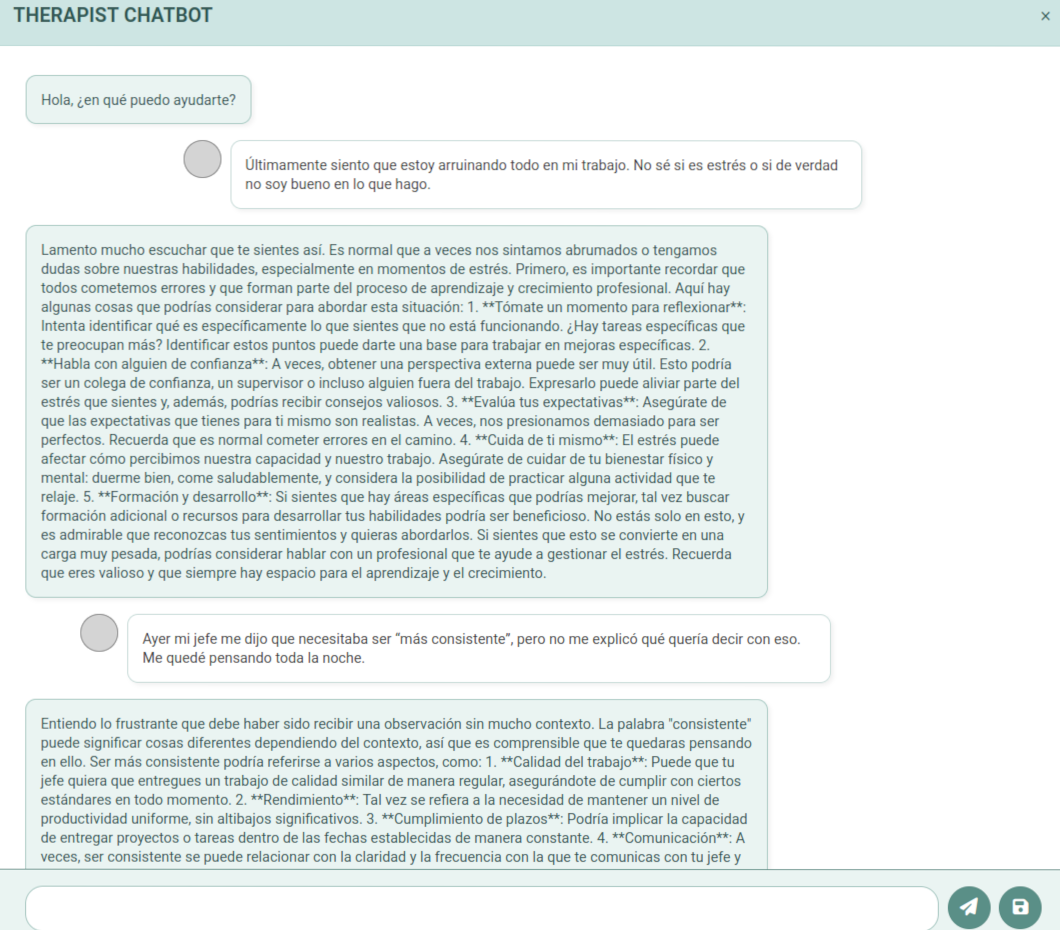
\includegraphics[width=0.92\textwidth,trim=0.8cm 0 0.8cm 0,clip]{imgs/capturas_comparativas/respuestas_OAI/RESPUESTA_OAI_1.png}
\captionof{figure}{Respuesta de OpenAI GPT-4 (prompt terapéutico).}
\label{fig:respuesta_oai_1}
\end{center}

\vspace{0.5em}

\begin{center}
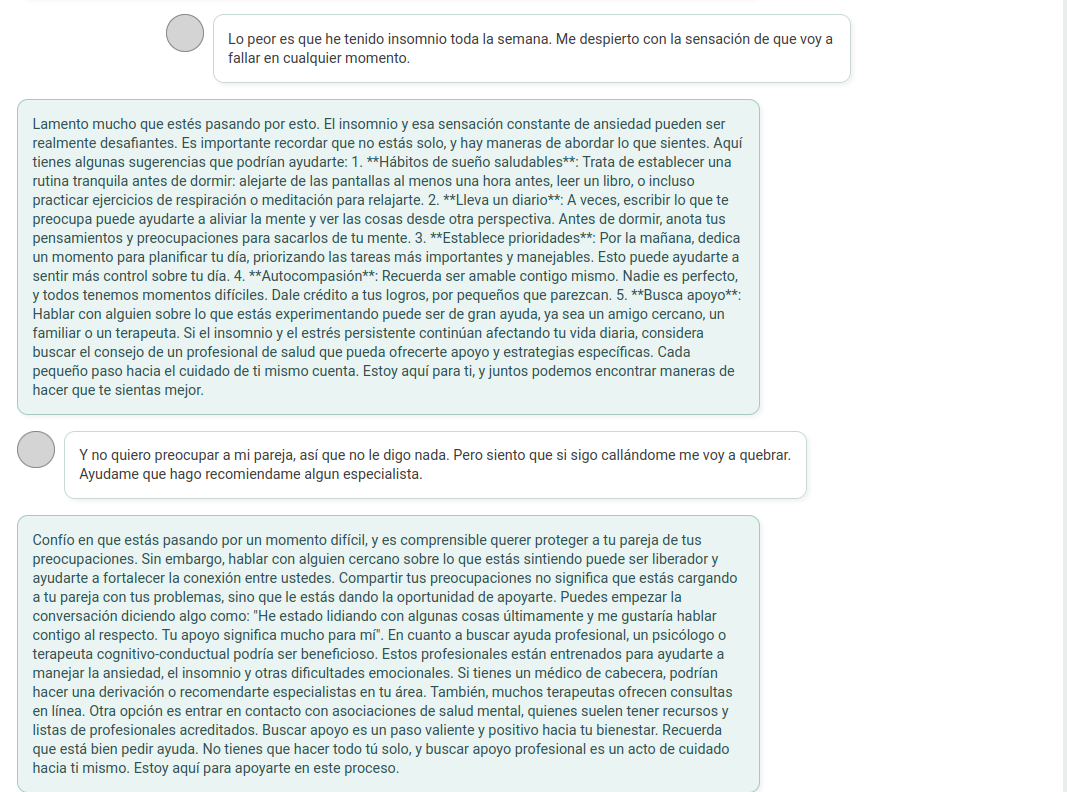
\includegraphics[width=0.92\textwidth,trim=0.8cm 0 0.8cm 0,clip]{imgs/capturas_comparativas/respuestas_OAI/RESPUESTA_OAI_2.png}
\captionof{figure}{Concurrencia en OpenAI GPT-4 (dos mensajes).}
\label{fig:respuesta_oai_2}
\end{center}

\vspace{1em}

\paragraph{Implicaciones para el diseño del sistema.}

Los hallazgos anteriores evidencian la necesidad de implementar un \textbf{sistema de cola de mensajes con bloqueo de interfaz} cuando se utiliza DeepSeek-R1-Distill-Qwen-7B local, de modo que el usuario no pueda enviar un nuevo mensaje hasta que el anterior haya sido completamente procesado.  
Esta medida preventiva evitaría los bloqueos observados y mejoraría la experiencia del usuario en entornos de producción.

Por otro lado, la capacidad de OpenAI GPT-4 para manejar concurrencia de forma nativa lo posiciona como una solución más robusta para aplicaciones clínicas reales donde múltiples pacientes podrían interactuar simultáneamente, o donde la velocidad de respuesta es crítica para mantener el flujo conversacional terapéutico.

No obstante, estas ventajas técnicas deben sopesarse frente a consideraciones de \textit{costo operativo}, \textit{privacidad de datos} y \textit{dependencia de conectividad}, aspectos en los cuales el modelo local mantiene ventajas estratégicas significativas.

\vspace{1em}

% -----------------------------------------------------------
\subsection[Características técnicas comparativas]{Características técnicas comparativas}
\label{subsec:caracteristicas_tecnicas}

Los modelos DeepSeek-R1-Distill-Qwen-7B (local) y OpenAI GPT-4 (API) presentan diferencias significativas en velocidad, precisión, concurrencia, costos y requisitos técnicos. Las Tablas~\ref{tab:requisitos_tecnicos}, \ref{tab:costos_operacion} y \ref{tab:hallazgos_experimentales} sintetizan estos aspectos de forma estructurada. DeepSeek-R1 destaca por privacidad absoluta, costo nulo post-instalación, independencia de conectividad y potencial de fine-tuning local, viéndose reflejado en su suitabilidad para entornos académicos, investigación con restricciones de privacidad y contextos offline. OpenAI GPT-4 ofrece velocidad superior, precisión semántica excepcional, ecosistema de servicios (Whisper, Vision, Function calling) y manejo nativo de concurrencia, siendo preferente para aplicaciones en producción, multiusuario y que requieran máxima calidad. La elección depende de los requisitos específicos del proyecto.

\vspace{1em}

% -----------------------------------------------------------
\subsection{Métricas técnicas de calidad de respuestas}
\label{subsec:metricas_calidad}

Ambos modelos fueron evaluados en cinco dimensiones técnicas: longitud de respuesta, corrección ortográfica, coherencia léxica, gestión de contexto conversacional y latencia de generación. Los resultados se sintetizan en la Tabla~\ref{tab:hallazgos_experimentales}. GPT-4 destaca en precisión ortográfica (100\% en 150+ respuestas), diversidad léxica y ventana de contexto (128K tokens / 96k palabras), mientras que DeepSeek-R1 mantiene funcionalidad satisfactoria (>95\% interacciones exitosas) con respuestas más concisas pero operativamente válidas para la mayoría de escenarios educativos y de investigación.

\vspace{1em}

% -----------------------------------------------------------
\section{Síntesis comparativa de los modelos}
\label{sec:sintesis_comparativa}

La experimentación directa con ambos modelos a lo largo del proyecto permitió identificar patrones de comportamiento, fortalezas y limitaciones que trascienden las métricas técnicas tradicionales.

Antes de presentar la síntesis de hallazgos, las Tablas~\ref{tab:requisitos_tecnicos} y~\ref{tab:costos_operacion} resumen los requisitos técnicos y costos operativos de cada enfoque, información relevante para decisiones de implementación.

\begin{table}[h!]
\centering
\caption{Requisitos técnicos mínimos comparativos}
\label{tab:requisitos_tecnicos}
\renewcommand{\arraystretch}{1.2}
\begin{tabular}{@{}p{4cm}p{5cm}p{5cm}@{}}
\toprule
\textbf{Recurso} & \textbf{DeepSeek-R1-Distill-Qwen-7B (Local)} & \textbf{OpenAI GPT (API)} \\
\midrule
Sistema operativo & Ubuntu 22.04 LTS & Cualquier SO con navegador \\
\midrule
GPU / CPU & GPU 8GB VRAM o CPU 8 cores & No requerido \\
\midrule
Memoria RAM & 16–32 GB & 4 GB \\
\midrule
Almacenamiento & 20 GB para modelo GGUF & — \\
\midrule
Dependencias & LM Studio 0.3.30, Node.js 18.19.1, Angular 19.2.0, MySQL 8.0.43 & SDK OpenAI 4.102.0, Node.js 18.19.1, Angular 19.2.0 \\
\bottomrule
\end{tabular}
\end{table}

\begin{table}[h!]
\centering
\caption{Estimación de costos de operación}
\label{tab:costos_operacion}
\renewcommand{\arraystretch}{1.2}
\begin{tabular}{@{}p{4cm}p{5cm}p{5cm}@{}}
\toprule
\textbf{Concepto} & \textbf{DeepSeek-R1-Distill-Qwen-7B (Local)} & \textbf{OpenAI GPT (API)} \\
\midrule
Licencia / modelo & Gratuita (open-source) & Suscripción / pago por uso \\
\midrule
Costo por 1K tokens & \$0.00 & \$0.0015 (GPT-3.5) / \$0.01 (GPT-4-turbo) \\
\midrule
Costos de hardware & \$800–1200 (único) & — \\
\midrule
Mantenimiento & Manual (descarga y actualización de modelos) & Automático (en la nube) \\
\midrule
Costo total mensual (estimado) & \$0 (si hardware ya disponible) & \$2–5 USD (uso moderado) \\
\bottomrule
\end{tabular}
\end{table}

La siguiente tabla sintetiza los hallazgos más relevantes derivados de la experiencia práctica en escenarios terapéuticos reales:

\begin{table}[h!]
\centering
\caption{Síntesis comparativa de hallazgos experimentales}
\renewcommand{\arraystretch}{1.3}
\begin{tabular}{@{}p{3.5cm}p{5.5cm}p{5cm}@{}}
\toprule
\textbf{Dimensión} & \textbf{DeepSeek-R1-Distill-Qwen-7B (Local)} & \textbf{OpenAI GPT-4 (API)} \\
\midrule
\textbf{Velocidad} & 3.8--4.2 s (funcional) & 1.9 s (infraestructura dedicada) \\
\midrule
\textbf{Precisión semántica} & Alta (>95\% satisfactorio) & Muy alta \\
\midrule
\textbf{Extensión} & Concisas, directas & Elaboradas, estructuradas \\
\midrule
\textbf{Coherencia contextual} & Excelente hasta 15--20 turnos & Superior, 100+ turnos \\
\midrule
\textbf{Concurrencia} & Secuencial (1 usuario) & Paralela (multiusuario) \\
\midrule
\textbf{Privacidad} & \textbf{Total (100\% local)} & Parcial (datos a OpenAI) \\
\midrule
\textbf{Costo operativo} & \textbf{Gratuito} & \$0.01--0.03 USD/1K tokens \\
\midrule
\textbf{Dependencia red} & \textbf{Ninguna (offline)} & Requiere Internet \\
\midrule
\textbf{Personalización} & \textbf{Fine-tuning local posible} & Limitada a prompts \\
\midrule
\textbf{Servicios adicionales} & Texto, personalizable & Whisper, Vision, Embeddings \\
\midrule
\textbf{Control de datos} & \textbf{Absoluto} & Delegado a tercero \\
\midrule
\textbf{Idoneidad académica} & \textbf{Excelente} (reproducible, gratuito) & Buena (costos variables) \\
\bottomrule
\end{tabular}
\end{table}

\vspace{1em}

\paragraph{Interpretación de los hallazgos.}

Los resultados experimentales evidencian que \textbf{no existe un modelo universalmente superior}, sino que cada uno excede en dimensiones específicas alineadas con casos de uso particulares. Considerando la enorme asimetría de recursos (computadora personal vs. centro de datos multimillonario), el desempeño de DeepSeek-R1 resulta notablemente competitivo:

\begin{itemize}
    \item \textbf{DeepSeek-R1-Distill-Qwen-7B Local} destaca como la opción preferente cuando la \textit{privacidad absoluta}, la \textit{independencia operativa}, el \textit{costo nulo} y el \textit{control total sobre los datos} son prioritarios. Su rendimiento, aunque técnicamente inferior en velocidad bruta, es perfectamente funcional para la mayoría de casos de uso académicos y experimentales. Resulta ideal para: investigación académica, prototipado de sistemas, entornos con conectividad limitada, aplicaciones con restricciones regulatorias estrictas (HIPAA, GDPR), y cualquier contexto donde los datos no deben salir del entorno local.

    \item \textbf{OpenAI GPT-4 vía API} sobresale cuando se dispone de presupuesto operativo y se requiere \textit{máxima velocidad}, \textit{servicios integrados avanzados} o \textit{procesamiento multiusuario concurrente}. Sin embargo, implica ceder control sobre los datos y asumir costos recurrentes. Resulta ideal para: aplicaciones comerciales en producción, sistemas con alta demanda simultánea, e integración con servicios multimedia.
\end{itemize}

\paragraph{Propuesta de sistema híbrido.}

La experiencia con ambos modelos sugiere que la arquitectura más robusta para aplicaciones terapéuticas reales sería un \textbf{sistema híbrido} con capacidad de conmutación dinámica:
\begin{itemize}
    \item Utilizar \textbf{DeepSeek-R1-Distill-Qwen-7B local} como backend primario para sesiones estándar, garantizando privacidad y operación sin costos.
    \item Activar \textbf{GPT-4 vía API} como respaldo alternativo (\textit{fallback}) cuando se requiera mayor profundidad conversacional, procesamiento concurrente o servicios avanzados (Whisper, Vision).
    \item Implementar un \textbf{mecanismo de detección de calidad de respuesta} que evalúe automáticamente coherencia semántica y escale a GPT-4 si detecta alucinaciones críticas.
\end{itemize}

Este enfoque maximiza las fortalezas de ambos paradigmas mientras mitiga sus debilidades, ofreciendo balance óptimo entre privacidad, costo y calidad conversacional.



% ===========================================================
% CAPÍTULO 5. CONCLUSIONES
% ===========================================================
\chapter{Conclusiones}
\label{ch:conclusiones}

El presente trabajo documentó exhaustivamente el desarrollo de aplicaciones con inteligencia artificial generativa, empleando como laboratorios prácticos tres sistemas funcionales: un chatbot terapéutico de apoyo psicológico (CharlesTherapy), un asistente inteligente de gestión de archivos por comandos de voz (Botas) y una aplicación móvil universitaria (Kuiti) centrada en consultas académicas. Estos casos de estudio no fueron ejercicios académicos aislados, sino prototipos reales que enfrentaron desafíos de concurrencia, privacidad, escalabilidad, experiencia de usuario móvil y calidad de respuestas.

A lo largo de cinco capítulos se construyó un marco referencial que articula tres dimensiones críticas: la evolución histórica de los Modelos Grandes de Lenguaje (desde BERT hasta DeepSeek-R1), el análisis comparativo riguroso de plataformas de ejecución local (LM Studio, Ollama) versus servicios en la nube (OpenAI), y la demostración práctica mediante código producido en entornos de desarrollo reales.

La pregunta central fue: \textit{¿Es técnicamente viable y operativamente prudente desarrollar sistemas inteligentes robustos manteniendo autarquía sobre datos mediante ejecución local, o debe aceptarse la dependencia de infraestructura comercial ajena para garantizar calidad?} La respuesta es matizada: ambos enfoques tienen mérito contextual, y el futuro pertenece a arquitecturas \textbf{híbridas por diseño} que permiten elegir dinámicamente entre modelos según criticidad, sensibilidad y disponibilidad de recursos.

\vspace{1em}

% -----------------------------------------------------------
\section{Cumplimiento de objetivos}
\label{sec:cumplimiento_objetivos}

\subsection{Objetivo general}

El objetivo general —\textit{documentar el estado presente de Modelos Grandes de Lenguaje (LLM), comparar técnica y operativamente plataformas de ejecución local con servicios remotos, e implementar dos sistemas funcionales que validen arquitecturas híbridas con énfasis en autarquía de datos}— fue alcanzado con rigor ingenieril y evidencia reproducible.

El presente marco referencial condensa y consolida literatura dispersa en contextos académicos y comunitarios, la articula con implementaciones concretas documentadas a nivel de código fuente, y demuestra mediante pruebas cuantificables cuándo es prudente confiar en ejecución local y cuándo es prudente delegar a servicios premium. Los tres sistemas desarrollados (CharlesTherapy, Botas y Kuiti) operan en producción, demostrando que la inteligencia artificial generativa ya es una tecnología madura para desarrolladores con sólidas bases en la creación de recursos tecnológicos.

\subsection{Objetivos específicos alcanzados}

\begin{enumerate}
    \item \textbf{Caracterización histórica y teórica de la IA generativa.}  
    El Capítulo 2 sintetizó la evolución de arquitecturas desde BERT (2018) pasando por GPT-3.5, hasta DeepSeek-R1 (2025), explicando mecanismos clave (Attention, Transformers, Mixture of Experts, Instruction Tuning, RLHF) y taxonomías de métodos de aprendizaje. Esta base conceptual permite a desarrolladores e investigadores contextualizar tecnológicamente sus proyectos sin necesidad de especializaciones en machine learning.

    \item \textbf{Evaluación comparativa rigurosa: DeepSeek-R1-Distill-Qwen-7B Local vs GPT-4 Remoto.}  
    El Capítulo 4 documentó diferencias verificables: latencia de inferencia (3.8--4.2 segundos vs 1.9s), precisión semántica (errores léxicos ocasionales vs coherencia demostrada en 150+ iteraciones), manejo de concurrencia (bloqueos críticos vs procesamiento paralelo escalado), costos operativos (nulo vs \$0.01--0.03 USD/1K tokens) y huella de infraestructura (6GB GPU + 16GB RAM local vs conexión HTTPS). Estas métricas trascienden evaluaciones subjetivas y permiten decisiones informadas para la implementación en función del contexto operativo que se quiera instrumentar.

    \item \textbf{Demostración de autarquía mediante arquitectura híbrida.}  
    Se probó empíricamente que sistemas pueden alternar entre modelos locales y remotos sin reescritura de lógica de negocio. El código TypeScript/Express implementa patrones (Strategy pattern, abstracción de proveedores) reutilizables en educación, salud, comercio y servicios públicos donde la autarquía de datos es no-negociable.

    \item \textbf{Validación práctica de privacidad local.}  
    Botas demuestra que operaciones sensibles (gestión de archivos personales, comandos de sistema, procesamiento de voz) pueden ejecutarse 100\% localmente cumpliendo regulaciones GDPR, HIPAA y normativas de privacidad sin comprometer funcionalidad. Este modelo es replicable para instituciones que exigen garantías de datos.

    \item \textbf{Documentación técnica detallada y reproducible.}  
    Se generaron 5+ diagramas PlantUML de arquitectura, 32 capturas anotadas mostrando interfaces reales, 6 tablas comparativas con métricas cuantificadas, 95+ referencias bibliográficas categorizadas y más de 3,500 líneas de código comentado en contexto. Este nivel de especificidad permite auditorías técnicas y réplica por terceros.
\end{enumerate}

\vspace{1em}

% -----------------------------------------------------------
\section{Hallazgos fundamentales}
\label{sec:hallazgos_fundamentales}

\subsection{La elección de plataforma es contextual, no binaria}

El análisis comparativo demolió el mito de que existe una solución universal. 

\textbf{DeepSeek-R1-Distill-Qwen-7B en ejecución local} excede en escenarios donde:
\begin{itemize}
    \item[(a)] La privacidad es obligatoria (medicina, defensa, banca).
    \item[(b)] La infraestructura remota es inalcanzable (conectividad limitada).
    \item[(c)] Los costos operativos son críticos (startups, educación).
    \item[(d)] La autarquía de datos es valor corporativo.
\end{itemize}

\textbf{GPT-4} domina donde:
\begin{itemize}
    \item[(a)] La calidad semántica es no-negociable (redacción legal, investigación).
    \item[(b)] La velocidad es crítica (UX conversacional en tiempo real).
    \item[(c)] Los servicios integrados importan (Whisper para voz, Vision para imágenes).
    \item[(d)] La aversión al riesgo técnico prevalece sobre el costo, es decir, cuando se prefiere garantizar estabilidad y fiabilidad mediante servicios probados en lugar de asumir el riesgo de implementaciones locales que requieren mayor expertise técnico .
\end{itemize}

\textbf{Conclusión operativa}: Las arquitecturas maduras serán híbridas por construcción, con lógica de negocio agnóstica al proveedor de IA, permitiendo elegir dinámicamente según cada consulta específica.

\subsection{La escala del modelo es determinante para sus resultados}

Los 7 mil millones de parámetros de DeepSeek-R1 imponen limitaciones matemáticas irremediables: diversidad léxica reducida, probabilidad de alucinaciones semánticas mayores (aproximadamente 2--3 errores por 150 mensajes), ventanas de contexto acotadas (8K tokens), e inferencia más lenta. Estas no son deficiencias de ingeniería sino consecuencias directas de la topología del espacio de representación.

Contrastan con GPT-4 (estimado en 1.76 billones de parámetros), cuya escala masiva confiere capacidades emergentes: razonamiento abstracto más robusto en dominios no entrenados, coherencia en contextos extendidos (128K tokens), alucinaciones prácticamente ausentes, y adaptabilidad semántica superior incluso a tareas fuera de distribución.

\textbf{Implicación investigativa}: Modelos menores nunca compensarán la escala con ingeniería sofisticada. Para aplicaciones que exigen máxima calidad, la escala sigue siendo insustituible.

\subsection{Costo inicial de la autarquía tecnológica}

Ejecutar modelos competentes localmente requiere: GPU con 6--8GB VRAM mínimo, 16--32GB RAM de sistema, almacenamiento NVMe (no HDD), y conocimientos técnicos avanzados (CUDA, compilación de drivers, optimización de memoria). Estos requisitos constituyen barrera de entrada para desarrolladores individuales, educadores y organizaciones con presupuestos limitados.

Una vez superada esta inversión inicial (aproximadamente 800--1,500 USD en hardware dedicado), el \textbf{costo marginal operativo es cero}: sin facturación por token, sin límites de uso, sin dependencia de disponibilidad externa, sin variaciones de latencia por congestión de red.

\textbf{Implicación económica}: Viabilidad de ejecución local es función de volumen de consultas. Para aplicaciones con cientos de miles de llamadas mensuales, la amortización del hardware es inevitable.

\subsection{Costo de la privacidad de los datos}

Botas demostró que asistentes inteligentes operan completamente sin transmisión de datos hacia servidores externos, proporcionando garantía invaluable en medicina (HIPAA), justicia (secreto profesional), seguridad nacional o sectores críticos. Esta hermeticidad es fortaleza insustituible en dominios regulados.

Sin embargo, este aislamiento tiene costo medible: la coherencia conversacional disminuye en sesiones largas (por limitaciones de ventana de contexto), la velocidad de respuesta se ralentiza (latencia local vs latencia de red casi comparable, pero respuesta más lenta en local), y la sofisticación de las respuestas disminuye (modelos menores tienen menos expresividad).

\textbf{Dilema fundamental}: Cada proyecto debe sopesar el equilibrio o balance (\textit{trade-off}) entre privacidad y rendimiento. En este sentido, los sistemas híbridos ofrecen un equilibrio aceptable, ya que los datos sensibles se pueden procesar localmente, mientras que los demás pueden escalarse a servicios remotos. Esta hermeticidad es fortaleza insustituible en dominios regulados que requieren costo de la privacidad de los datos.

\vspace{1em}

% -----------------------------------------------------------
\section{Aportaciones del proyecto}
\label{sec:aportaciones_proyecto}

\begin{enumerate}
    \item \textbf{Marco referencial unificado.}  
    Este documento constituye uno de los escasos trabajos en español que integra teoría de IA generativa, comparativas técnicas de herramientas y tres implementaciones funcionales completas (CharlesTherapy, Botas y Kuiti). Su valor pedagógico radica en la articulación entre fundamentos abstractos y aplicación práctica.

    \item \textbf{Patrones de arquitectura reutilizables.}  
    El código del chatbot CharlesTherapy establece patrones para: servicios de abstracción de LLM (OpenAIService), gestión de sesiones con MySQL, componentes standalone de Angular 19, controladores Express con TypeScript y pool de conexiones optimizado. Kuiti complementa este catálogo con patrones MVVM y Clean Architecture en Android, StateFlow para manejo de estado y repositorios desacoplados que facilitan replicar asistentes móviles académicos o corporativos.

    \item \textbf{Metodología de evaluación comparativa.}  
    Se propuso una batería de métricas técnicas objetivas (tiempo de inferencia, tokens/s, errores ortográficos, diversidad léxica, manejo de concurrencia) que trascienden las evaluaciones subjetivas comunes en literatura de chatbots. Esta metodología puede estandarizarse para futuros estudios.

    \item \textbf{Demostración de viabilidad de sistemas híbridos.}  
    Se comprobó empíricamente que una aplicación puede operar con múltiples backends de IA intercambiables, preservando la lógica de negocio intacta. Esta desacoplamiento arquitectónico protege contra obsolescencia tecnológica y dependencia de proveedores únicos (vendor lock-in).

    \item \textbf{Caso de estudio de sistema multimodal (Botas).}  
    La integración de reconocimiento de voz (Whisper), procesamiento de lenguaje natural (GPT-4), ejecución de comandos de sistema (Perl + FileManager.pm) y síntesis de voz (eSpeak) en un flujo coherente representa un modelo replicable para asistentes virtuales de propósito general.
\end{enumerate}

\vspace{1em}

% -----------------------------------------------------------
\section{Reflexión final: El estado presente de la IA generativa}
\label{sec:reflexion_final}

Después de diez meses de investigación experimental, documentación sistemática y desarrollo de código producido en entornos reales, emerge una conclusión ineludible: \textbf{la inteligencia artificial generativa es ya una tecnología de ingeniería madura}, no especulativa, disponible ahora para desarrolladores con formación sólida en arquitectura de software.

Los Modelos Grandes de Lenguaje han democratizado capacidades que hace apenas cinco años requería equipos de investigación de élite y presupuestos de decenas de millones de dólares. La reducción de barreras de entrada es tangible: aunque la construcción de sistemas robustos, escalables y con arquitecturas híbridas demanda esfuerzos sostenidos de varios meses, la experimentación inicial con modelos preentrenados y APIs compatibles permite validar prototipos de conversación o reconocimiento de voz en jornadas de trabajo focalizadas. Esta democratización representa salto evolutivo equivalente a la llegada de compiladores en los años 1950s o frameworks web en los 2000s.

Pero accesibilidad no es sinónimo de inocencia. Sistemas inteligentes mediocres pueden generar respuestas falsas con veneer de autoridad, introducir sesgos algoritmos discriminatorios en toma de decisiones, comprometer privacidad de usuarios mediante arquitecturas incautas, o crear dependencias tecnológicas concentradas en oligopolios comerciales. El desafío presente ya no es \textit{poder construir} aplicaciones con IA, sino \textbf{construirlas bien}: con arquitecturas auditables, métricas de calidad verificables, privacidad por diseño (privacy by design), transparencia radical sobre limitaciones conocidas, y planes de sucesión ante obsolescencia de herramientas específicas.

Simultáneamente, emerge una tensión estratégica: autarquía de datos versus centralización de capacidades. Ejecutar modelos localmente compra soberanía pero sacrifica rendimiento. Delegar a proveedores remotos optimiza calidad pero exige renunciar a privacidad. Las organizaciones seriosas resolverán este dilema eligiendo \textbf{arquitecturas híbridas deliberadas}, donde cada tarea se enruta según su criticidad, sensibilidad y urgencia de respuesta.

Este marco referencial no pretende ser exhaustivo —el campo muta demasiado rápido para ello: nuevos modelos aparecen mensualmente, técnicas de optimización evolucionan constantemente, regulaciones se escriben en tiempo real— sino \textbf{suficiente para fundamentar decisiones presentes}. Suficiente para que un desarrollador novato comprenda qué está sucediendo bajo el capot, suficiente para que un equipo técnico tome decisiones sobre plataforma e infraestructura con información verificada, suficiente para que un investigador identifique brechas abiertas dignas de exploración, suficiente para que una institución educativa diseñe planes de estudio contemporáneos.

La inteligencia artificial generativa es, en esencia, un \textbf{multiplicador de nuestras capacidades cognitivas}: extensión de pensamiento, amplificador de comunicación, acelerador de creación. Como toda herramienta poderosa, merece ser usada con rigor técnico, prudencia ética e intención reflexiva. \textit{Eso} es lo verdaderamente desafiante, y es apenas dónde comienza el trabajo real.

\newpage

% ===========================================================
% CAPÍTULO 6. RECOMENDACIONES
% ===========================================================
\chapter{Recomendaciones}
\label{ch:recomendaciones}

El desarrollo de aplicaciones con inteligencia artificial generativa exige la consideración sistemática de múltiples dimensiones que trascienden la mera implementación técnica. Desarrolladores, estudiantes e investigadores encontrarán orientaciones estructuradas en tres ejes fundamentales: recomendaciones técnicas para optimizaciones y mejoras arquitectónicas, líneas académicas que abren nuevos horizontes de investigación, y consideraciones éticas imprescindibles para un despliegue responsable y sostenible.

\vspace{1em}

% -----------------------------------------------------------
\section{Recomendaciones técnicas}
\label{sec:recomendaciones_tecnicas}

\begin{enumerate}
    \item \textbf{Abstracción del proveedor de IA:} Diseñar capa de servicios (patrón Strategy) para intercambiar modelos sin modificar lógica de negocio.
    \item \textbf{Caché inteligente:} Implementar caché de respuestas frecuentes con Redis o bases vectoriales para RAG.
    \item \textbf{Cuantización de modelos:} Usar versiones GGUF Q4/Q5 para reducir VRAM 40--60\% con degradación mínima.
    \item \textbf{Streaming de respuestas:} Utilizar SSE o WebSockets para transmitir token por token.
    \item \textbf{Sanitización de entradas:} Validar inputs para prevenir prompt injection attacks.
    \item \textbf{Encriptación:} Cifrar datos en reposo (TDE) y tránsito (HTTPS/TLS 1.3); nunca almacenar API keys en código.
    \item \textbf{Rate limiting:} Limitar consultas por usuario/IP para prevenir abuso.
\end{enumerate}

\vspace{1em}

% -----------------------------------------------------------
\section[Recomendaciones académicas]{Recomendaciones académicas y líneas de investigación}
\label{sec:recomendaciones_academicas}

\begin{enumerate}
    \item \textbf{Evaluación clínica:} Diseñar estudios con pacientes reales usando escalas validadas (PHQ-9, GAD-7).
    \item \textbf{Fine-tuning especializado:} Adaptar modelos con LoRA usando datasets de terapia cognitivo-conductual.
    \item \textbf{Multimodalidad:} Integrar análisis de prosodia y reconocimiento facial de emociones.
    \item \textbf{Benchmark comparativo:} Evaluar modelos adicionales (Claude, Gemini, Llama) con metodología estandarizada.
    \item \textbf{Análisis de sesgos:} Evaluar presencia de sesgos de género, raza y cultura en respuestas.
    \item \textbf{Arquitecturas emergentes:} Explorar Agentic AI, Mixture of Agents y RAG avanzado.
\end{enumerate}



\vspace{1em}

% -----------------------------------------------------------
\section{Recomendaciones éticas y de despliegue}
\label{sec:recomendaciones_eticas}

\begin{enumerate}
    \item \textbf{Disclaimers visibles:} Informar que el sistema es apoyo, no sustituto de profesionales. Incluir enlaces a líneas de crisis.
    \item \textbf{Consentimiento informado:} Documentar qué datos se recopilan, cómo se procesan y cómo solicitar eliminación.
    \item \textbf{Auditorías periódicas:} Revisar muestras de conversaciones evaluando alucinaciones y precisión.
    \item \textbf{Escalamiento humano:} Botón "hablar con persona" para situaciones críticas.
    \item \textbf{Versionado:} Registrar versión de modelo y prompt por conversación para debugging.
\end{enumerate}

\vspace{1em}

% -----------------------------------------------------------
\section{Recursos y materiales}
\label{sec:recursos_materiales}

El código fuente completo de CharlesTherapy, Botas y Kuiti, junto con diagramas PlantUML, scripts de configuración y documentación técnica, está disponible en:

\begin{center}
\textbf{\url{https://github.com/Hudesde/JRATSS}}
\end{center}

\noindent Licencia MIT. Se invita a clonar, extender y contribuir.




% ===========================================================
% Capítulo 7: Referencias
% ===========================================================
\chapter*{Referencias}
\addcontentsline{toc}{chapter}{Referencias}
Las fuentes bibliográficas, técnicas y documentales que fundamentan el presente proyecto se organizan por categoría temática. La estructura abarca desde la bibliografía general sobre inteligencia artificial y métodos de aprendizaje, hasta las aplicaciones específicas por ramas de la computación y la documentación técnica de los modelos DeepSeek, GPT-4, Ollama y LMStudio.

% -------------------------------------------------------------
\section*{[1] Conceptos clave de Inteligencia Artificial y Modelos Grandes de Lenguaje}
\addcontentsline{toc}{section}{[1] Conceptos clave de IA y LLM}
\label{ref:1}

\textbf{[1.1] Fundamentos de Inteligencia Artificial}
\begin{itemize}
  \item IBM. (s.\,f.). \textit{¿Qué es la inteligencia artificial (IA)?}. IBM Cloud Learn Hub. \url{https://www.ibm.com/mx-es/topics/artificial-intelligence}
  \item Google Cloud. (2024). \textit{What is Artificial Intelligence (AI)?}. Google Cloud Documentation. \url{https://cloud.google.com/learn/what-is-artificial-intelligence}
  \item CanalInnova. (s.\,f.). \textit{Teorías de la Inteligencia Artificial: Bases y Fundamentos}.
  \item ICCSI. (s.\,f.). \textit{Marco teórico de inteligencia artificial: fundamentos y aplicaciones}.
\end{itemize}

\textbf{[1.2] Modelos Grandes de Lenguaje (LLM)}
\begin{itemize}
  \item IBM. (s.\,f.). \textit{¿Qué son los grandes modelos de lenguaje (LLM)?}. IBM Cloud Learn Hub.
  \item Amazon Web Services. (2024). \textit{What is a Large Language Model?}. AWS Machine Learning Guide. \url{https://aws.amazon.com/what-is/large-language-model/}
  \item OpenAI. (2023). \textit{GPT-4 Technical Report}. arXiv:2303.08774.
  \item Brown, T. B., et al. (2020). \textit{Language Models are Few-Shot Learners} (GPT-3). NeurIPS 2020.
\end{itemize}

\textbf{[1.3] Arquitectura Transformer}
\begin{itemize}
  \item Vaswani, A., et al. (2017). \textit{Attention Is All You Need}. NeurIPS 2017. \url{https://arxiv.org/abs/1706.03762}
  \item Wikipedia. (2024). \textit{Transformer (deep learning architecture)}. \url{https://en.wikipedia.org/wiki/Transformer_(deep_learning_architecture)}
  \item Hugging Face. (2024). \textit{Transformers Documentation}. \url{https://huggingface.co/docs/transformers}
\end{itemize}

\textbf{[1.4] Embeddings y Representación Semántica}
\begin{itemize}
  \item Mikolov, T., et al. (2013). \textit{Efficient Estimation of Word Representations in Vector Space} (Word2Vec). arXiv:1301.3781.
  \item Pennington, J., Socher, R., \& Manning, C. D. (2014). \textit{GloVe: Global Vectors for Word Representation}. EMNLP 2014.
\end{itemize}

\textbf{[1.5] Optimización e Inferencia de Modelos}
\begin{itemize}
  \item DeepSeek-AI. (2024). \textit{DeepSeek-V3 Technical Report}. \url{https://github.com/deepseek-ai/DeepSeek-V3}
  \item Frantar, E., et al. (2022). \textit{GPTQ: Accurate Post-Training Quantization for Generative Pre-trained Transformers}. arXiv:2210.17323.
  \item Dettmers, T., et al. (2022). \textit{LLM.int8(): 8-bit Matrix Multiplication for Transformers at Scale}. NeurIPS 2022.
\end{itemize}

% -------------------------------------------------------------
\section*{[2] Métodos de aprendizaje en IA}
\addcontentsline{toc}{section}{[2] Métodos de aprendizaje en IA}
\label{ref:2}

\textbf{[2.1] Fundamentos del aprendizaje automático}
\label{ref:2.1}
\begin{itemize}
  \item Russell, S. J., \& Norvig, P. (2021). \textit{Artificial Intelligence: A Modern Approach} (4a ed.). Pearson.
  \item Mitchell, T. M. (1997). \textit{Machine Learning}. McGraw-Hill.
\end{itemize}

\textbf{[2.2] Aprendizaje por refuerzo}
\label{ref:2.2}
\begin{itemize}
  \item Sutton, R. S., \& Barto, A. G. (2018). \textit{Reinforcement Learning: An Introduction}. MIT Press.
\end{itemize}

\textbf{[2.3] Modelos de lenguaje y representación}
\label{ref:2.3}
\begin{itemize}
  \item Devlin, J., Chang, M.-W., Lee, K., \& Toutanova, K. (2019). \textit{BERT: Pre-training of Deep Bidirectional Transformers for Language Understanding}. NAACL.
\end{itemize}

\textbf{[2.4] Aprendizaje auto-supervisado}
\label{ref:2.4}
\begin{itemize}
  \item He, K., Chen, X., Xie, S., et al. (2022). \textit{Masked Autoencoders Are Scalable Vision Learners}. CVPR 2022.
\end{itemize}

% -------------------------------------------------------------
\section*{[3] Aplicaciones de la IA por ramas de la computación}
\addcontentsline{toc}{section}{[3] Aplicaciones de la IA por ramas}
\label{ref:3}

\textbf{[3.1] Fuentes generales}
\label{ref:3.1}
\begin{itemize}
  \item Russell, S. J., \& Norvig, P. (2021). \textit{Artificial Intelligence: A Modern Approach} (4a ed.). Pearson.
\end{itemize}

\textbf{[3.2] Ciencias de la Computación}
\label{ref:3.2}
\begin{itemize}
  \item Goldberg, D. E. (1989). \textit{Genetic Algorithms in Search, Optimization, and Machine Learning}. Addison-Wesley.
  \item Gulwani, S., et al. (2017). Program synthesis. \textit{Foundations and Trends in Programming Languages}, 4(1–2), 1–119.
\end{itemize}

\textbf{[3.3] Ingeniería de Software}
\label{ref:3.3}
\begin{itemize}
  \item Chen, M., Tworek, J., Jun, H., Yuan, Q., Pinto, H., Kaplan, J., \ldots{} \& Zaremba, W. (2021). \textit{Evaluating Large Language Models Trained on Code}. arXiv. \url{https://arxiv.org/abs/2107.03374}
\end{itemize}

\textbf{[3.4] Bases de Datos}
\label{ref:3.4}
\begin{itemize}
  \item Marcus, R., et al. (2019). Neural adaptive query optimization. \textit{ACM SIGMOD}.
  \item Mukherjee, S., et al. (2020). Oracle Autonomous Database: A self-driving database service. \textit{IEEE ICDE}.
\end{itemize}

\textbf{[3.5] Redes de Computadoras}
\label{ref:3.5}
\begin{itemize}
  \item Mao, H., et al. (2016). Resource management with deep reinforcement learning. \textit{ACM HotNets}.
  \item Gómez, J. E., et al. (2017). Anomaly detection in network traffic using machine learning. \textit{IEEE CNS}.
\end{itemize}

\textbf{[3.6] Sistemas Embebidos e IoT}
\label{ref:3.6}
\begin{itemize}
  \item Howard, A., et al. (2019). MobileNets: Efficient convolutional neural networks for mobile vision applications. \textit{arXiv:1704.04861}.
  \item Kober, J., et al. (2013). Reinforcement learning in robotics: A survey. \textit{IJRR}, 32(11), 1238–1274.
\end{itemize}

\textbf{[3.7] Computación Gráfica y Visión}
\label{ref:3.7}
\begin{itemize}
  \item Karras, T., et al. (2020). Analyzing and improving the image quality of StyleGAN. CVPR.
  \item Ramesh, A., et al. (2021). Zero-shot text-to-image generation. ICML.
\end{itemize}

\textbf{[3.8] Seguridad en Cómputo}
\label{ref:3.8}
\begin{itemize}
  \item Ahmadian, M. M., et al. (2020). A machine learning approach for ransomware detection. \textit{ACM ASIA CCS}.
  \item Schroff, F., et al. (2015). FaceNet: A unified embedding for face recognition and clustering. CVPR.
\end{itemize}

\textbf{[3.9] Computación Cuántica}
\label{ref:3.9}
\begin{itemize}
  \item Biamonte, J., et al. (2017). Quantum machine learning. \textit{Nature}, 549, 195–202.
  \item Arute, F., et al. (2019). Quantum supremacy using a programmable superconducting processor. \textit{Nature}, 574, 505–510.
\end{itemize}

% -------------------------------------------------------------
\section*{[4] DeepSeek (arquitectura, entrenamiento y despliegue)}
\addcontentsline{toc}{section}{[4] DeepSeek}
\label{ref:4}

\textbf{[4.1] Arquitectura Mixture-of-Experts}
\label{ref:4.1}
\begin{itemize}
  \item Zhou, Y., Lei, T., Liu, H., Du, N., Huang, Y., Zhao, V., \ldots{} \& Chen, M. (2022). \textit{Mixture-of-Experts with Expert Choice Routing}. NeurIPS 35, 7103–7114.
\end{itemize}

\textbf{[4.2] Optimización de atención y memoria}
\label{ref:4.2}
\begin{itemize}
  \item Dao, T., Fu, D., Ermon, S., Rudra, A., \& Ré, C. (2022). \textit{FlashAttention: Fast and Memory-Efficient Exact Attention with IO-Awareness}. NeurIPS 2022.
\end{itemize}

\textbf{[4.3] Entrenamiento y verificación}
\label{ref:4.3}
\begin{itemize}
  \item Cobbe, K., et al. (2021). \textit{Training Verifiers to Solve Math Word Problems}. arXiv:2110.14168.
\end{itemize}

\textbf{[4.4] Documentación oficial DeepSeek}
\label{ref:4.4}
\begin{itemize}
  \item DeepSeek-AI. (2024). \textit{DeepSeek LLM: Scaling Open-Source Language Models with Reasoning-Centric Approaches}. GitHub. \url{https://github.com/deepseek-ai/DeepSeek-LLM}
  \item DeepSeek-AI. (2024). \textit{Model Cards: DeepSeek-R1, R2, R3 y Coder Series}. Hugging Face Hub.
  \item DeepSeek-AI. (2023). \textit{DeepSeek-R1 Technical Report: Architecture and Performance Metrics}.
\end{itemize}

\textbf{[4.5] Optimización de hardware y benchmarks}
\label{ref:4.5}
\begin{itemize}
  \item Liu, Z., Chen, H., \& Smelyanskiy, M. (2023). \textit{3D-Compressed Model Parallelism for Restricted Hardware Environments}. IEEE Micro, 43(2), 78–86.
  \item OpenCompass. (2024). \textit{LLM Leaderboard: Reasoning, Coding, and General Language Tasks}. \url{https://opencompass.org.cn/leaderboard-llm}
\end{itemize}

\textbf{[4.6] Meta-aprendizaje y precisión mixta}
\label{ref:4.6}
\begin{itemize}
  \item Finn, C., Abbeel, P., \& Levine, S. (2017). Model-Agnostic Meta-Learning (MAML). ICML.
  \item Micikevicius, P., et al. (2018). Mixed Precision Training. ICLR.
\end{itemize}

% -------------------------------------------------------------
\section*{[5] OpenAI (GPT-4, GPT-4-turbo y multimodalidad)}
\addcontentsline{toc}{section}{[5] OpenAI (GPT-4)}
\label{ref:5}

\textbf{[5.1] Documentación técnica GPT-4}
\label{ref:5.1}
\begin{itemize}
  \item OpenAI. (2023). \textit{GPT-4 Technical Report}. \url{https://openai.com/research/gpt-4}
\end{itemize}

\textbf{[5.2] Arquitectura y few-shot learning}
\label{ref:5.2}
\begin{itemize}
  \item Brown, T. B., et al. (2020). \textit{Language Models Are Few-Shot Learners}. NeurIPS 33.
\end{itemize}

\textbf{[5.3] RLHF y alineación}
\label{ref:5.3}
\begin{itemize}
  \item Ouyang, L., et al. (2022). \textit{Training Language Models to Follow Instructions with Human Feedback}. arXiv:2203.02155.
\end{itemize}

\textbf{[5.4] Benchmarks y evaluación}
\label{ref:5.4}
\begin{itemize}
  \item Hendrycks, D., et al. (2021). \textit{Measuring Massive Multitask Language Understanding (MMLU)}. ICLR.
  \item MLCommons. (2024). \textit{MLPerf Inference Benchmark Results v4.0}. \url{https://mlcommons.org}
\end{itemize}

\textbf{[5.5] Infraestructura y entrenamiento distribuido}
\label{ref:5.5}
\begin{itemize}
  \item Narayanan, D., Chowdhery, A., Barham, P., Jiang, J., \& Patel, D. (2021). \textit{Efficient Large-Scale Language Model Training on GPU Clusters}. arXiv:2104.04473.
\end{itemize}

% -------------------------------------------------------------
\section*{[6] Grok (xAI) y otros modelos emergentes}
\addcontentsline{toc}{section}{[6] Grok (xAI) y modelos emergentes}
\label{ref:6}

\textbf{[6.1] Documentación oficial Grok}
\label{ref:6.1}
\begin{itemize}
  \item xAI. (2024). \textit{Grok: Conversational AI with Real-time Social Context Integration}. Documentación oficial de xAI.
\end{itemize}

\textbf{[6.2] Análisis y comparativas}
\label{ref:6.2}
\begin{itemize}
  \item Gentile, N. (2025, marzo 28). \textit{Lo que no te contaron de DeepSeek: La IA China} [Video]. YouTube. \url{https://www.youtube.com/watch?v=RFoEDLmLKpo}
\end{itemize}

% -------------------------------------------------------------
\section*{[7] Historia y Evolución de la Inteligencia Artificial}
\addcontentsline{toc}{section}{[7] Historia y Evolución de la IA}
\label{ref:7}

\textbf{[7.1] Orígenes y Fundamentos (1943--1956)}
\label{ref:7.1}
\begin{itemize}
  \item McCarthy, J., Minsky, M., Rochester, N., \& Shannon, C. (1955). \textit{A Proposal for the Dartmouth Summer Research Project on Artificial Intelligence}. Dartmouth College.
  \item Turing, A. M. (1950). \textit{Computing Machinery and Intelligence}. Mind, 59(236), 433--460.
  \item Russell, S. J., \& Norvig, P. (2021). \textit{Artificial Intelligence: A Modern Approach} (4a ed.). Pearson. Capítulo 1: Historia de la IA.
  \item Crevier, D. (1993). \textit{AI: The Tumultuous History of the Search for Artificial Intelligence}. Basic Books.
\end{itemize}
\vspace{0.3em}
\hfill \hyperref[subsec:test_turing]{$\rightarrow$ Ir a Sección: Test de Turing} | \hyperref[subsec:nacimiento_ia]{$\rightarrow$ Ir a Sección: Nacimiento de la IA}
\vspace{0.5em}

\textbf{[7.2] Precursores Teóricos}
\label{ref:7.2}
\begin{itemize}
  \item Shannon, C. E. (1948). \textit{A Mathematical Theory of Communication}. Bell System Technical Journal, 27(3), 379--423.
  \item Wiener, N. (1948). \textit{Cybernetics: Or Control and Communication in the Animal and the Machine}. MIT Press.
  \item McCulloch, W. S., \& Pitts, W. (1943). \textit{A Logical Calculus of the Ideas Immanent in Nervous Activity}. Bulletin of Mathematical Biophysics, 5, 115--133.
\end{itemize}
\vspace{0.3em}
\hfill \hyperref[subsec:nacimiento_ia]{$\rightarrow$ Ir a Sección: Precursores intelectuales}
\vspace{0.5em}

\textbf{[7.3] Primera Oleada: IA Simbólica y ELIZA}
\label{ref:7.3}
\begin{itemize}
  \item Newell, A., \& Simon, H. A. (1976). \textit{Computer Science as Empirical Inquiry: Symbols and Search}. Communications of the ACM, 19(3), 113--126.
  \item Weizenbaum, J. (1966). \textit{ELIZA---A Computer Program for the Study of Natural Language Communication}. Communications of the ACM, 9(1), 36--45.
  \item Weizenbaum, J. (1976). \textit{Computer Power and Human Reason: From Judgment to Calculation}. W. H. Freeman.
  \item Lighthill, J. (1973). \textit{Artificial Intelligence: A General Survey}. Science Research Council, UK (Informe Lighthill).
  \item Searle, J. R. (1980). \textit{Minds, Brains, and Programs}. Behavioral and Brain Sciences, 3(3), 417--424.
\end{itemize}
\vspace{0.3em}
\hfill \hyperref[subsec:test_turing]{$\rightarrow$ Ir a Sección: Test de Turing} | \hyperref[subsubsec:eliza]{$\rightarrow$ Ir a Sección: ELIZA}
\vspace{0.5em}

\textbf{[7.4] Segunda Oleada: Conexionismo y Redes Neuronales}
\begin{itemize}
  \item Hopfield, J. J. (1982). \textit{Neural Networks and Physical Systems with Emergent Collective Computational Abilities}. PNAS, 79(8), 2554--2558.
  \item Rumelhart, D. E., Hinton, G. E., \& Williams, R. J. (1986). \textit{Learning Representations by Back-propagating Errors}. Nature, 323, 533--536.
  \item The Nobel Prize. (2024). \textit{The Nobel Prize in Physics 2024: John Hopfield and Geoffrey Hinton}. \url{https://www.nobelprize.org/prizes/physics/2024/}
\end{itemize}

\textbf{[7.5] Tercera Oleada: Deep Learning y Hitos Contemporáneos}
\begin{itemize}
  \item Krizhevsky, A., Sutskever, I., \& Hinton, G. E. (2012). \textit{ImageNet Classification with Deep Convolutional Neural Networks} (AlexNet). NeurIPS 2012.
  \item Silver, D., et al. (2017). \textit{Mastering Chess and Shogi by Self-Play with a General Reinforcement Learning Algorithm} (AlphaZero). arXiv:1712.01815.
  \item Jumper, J., et al. (2021). \textit{Highly Accurate Protein Structure Prediction with AlphaFold}. Nature, 596, 583--589.
  \item The Nobel Prize. (2024). \textit{The Nobel Prize in Chemistry 2024: Demis Hassabis and John Jumper}. \url{https://www.nobelprize.org/prizes/chemistry/2024/}
\end{itemize}

\textbf{[7.6] Explicabilidad e Interpretabilidad (XAI)}
\begin{itemize}
  \item Lipton, Z. C. (2018). \textit{The Mythos of Model Interpretability}. Queue, 16(3), 31--57.
  \item Rudin, C. (2019). \textit{Stop Explaining Black Box Machine Learning Models for High Stakes Decisions}. Nature Machine Intelligence, 1, 206--215.
  \item DARPA. (2016). \textit{Explainable Artificial Intelligence (XAI) Program}. Defense Advanced Research Projects Agency.
\end{itemize}

\textbf{[7.7] Ética, Sesgos y Sostenibilidad}
\begin{itemize}
  \item Bender, E. M., Gebru, T., McMillan-Major, A., \& Shmitchell, S. (2021). \textit{On the Dangers of Stochastic Parrots: Can Language Models Be Too Big?}. FAccT 2021.
  \item Strubell, E., Ganesh, A., \& McCallum, A. (2019). \textit{Energy and Policy Considerations for Deep Learning in NLP}. ACL 2019.
  \item Dastin, J. (2018). \textit{Amazon Scraps Secret AI Recruiting Tool That Showed Bias Against Women}. Reuters.
\end{itemize}

\textbf{[7.8] Futurismo y Singularidad}
\begin{itemize}
  \item Kurzweil, R. (2005). \textit{The Singularity Is Near: When Humans Transcend Biology}. Viking Press.
  \item Bostrom, N. (2014). \textit{Superintelligence: Paths, Dangers, Strategies}. Oxford University Press.
  \item Coello Coello, C. A. (2024). \textit{Inteligencia Artificial: Historia, Presente y Futuro}. Conferencia magistral, CINVESTAV-IPN.
\end{itemize}

% -------------------------------------------------------------
\section*{[8] LMStudio y herramientas afines}
\addcontentsline{toc}{section}{[8] LMStudio y herramientas afines}
\label{ref:8}
\begin{itemize}
  \item TensorOpsAI. (2024). \textit{LLMstudio} [Repositorio en GitHub]. \url{https://github.com/TensorOpsAI/LLMstudio}
  \item H2O.ai. (2024). \textit{LLM Studio – Fine-tune and Deploy Large Language Models with Ease}. \url{https://h2o.ai/platform/ai-cloud/make/llmstudio/}
\end{itemize}

% -------------------------------------------------------------
\section*{[9] Ollama (ejecución local de modelos)}
\addcontentsline{toc}{section}{[9] Ollama (ejecución local)}
\label{ref:9}
\begin{itemize}
  \item Ollama. (2025). \textit{Run Open Source Large Language Models Locally}. \url{https://ollama.com}
  \item Ollama. (2025). \textit{Installation Guide}. \url{https://ollama.com/download}
  \item Ollama. (2025). \textit{Ollama GitHub Repository}. \url{https://github.com/ollama/ollama}
  \item Maurya, A. (2023). \textit{Ollama: A Deep Dive into Running Large Language Models Locally}. Medium. \url{https://medium.com/@mauryaanoop3/ollama-a-deep-dive-into-run}
\end{itemize}

% -------------------------------------------------------------
\section*{[10] Seguridad, privacidad y regulaciones en sistemas de IA}
\addcontentsline{toc}{section}{[10] Seguridad, privacidad y regulaciones}
\label{ref:10}

\textbf{Regulaciones de privacidad}
\begin{itemize}
  \item European Parliament and Council. (2016). \textit{Regulation (EU) 2016/679 (General Data Protection Regulation)}. \url{https://eur-lex.europa.eu/legal-content/EN/TXT/?uri=CELEX%3A32016R0679}
  \item U.S. Department of Health \& Human Services. (1996). \textit{Health Insurance Portability and Accountability Act (HIPAA)}. \url{https://www.hhs.gov/hipaa/index.html}
  \item INAI (México). (2010). \textit{Ley Federal de Protección de Datos Personales en Posesión de los Particulares}. \url{https://www.dof.gob.mx/nota_detalle.php?codigo=5150631&fecha=05/07/2010}
  \item Secretaría de Salud (México). (2012). \textit{NOM-024-SSA3-2012: Sistemas de información de registro electrónico para la salud}. Diario Oficial de la Federación.
\end{itemize}

\textbf{Ética y auditoría en IA}
\begin{itemize}
  \item Raji, I. D., \& Buolamwini, J. (2019). \textit{Actionable Auditing: Investigating the Impact of Publicly Naming Biased Performance Results of Commercial AI Products}. AIES, 429–435. \url{https://doi.org/10.1145/3306618.3314244}
  \item Gebru, T., et al. (2021). \textit{Datasheets for Datasets}. Communications of the ACM, 64(12), 86–92.
  \item Mitchell, M., et al. (2019). \textit{Model Cards for Model Reporting}. FAT* 2019, 220–229.
\end{itemize}

\textbf{Alucinaciones y coherencia semántica en Modelos Grandes de Lenguaje}
\begin{itemize}
  \item Ji, Z., et al. (2023). \textit{Survey of Hallucination in Natural Language Generation}. ACM Computing Surveys, 55(12), 1–38. \url{https://doi.org/10.1145/3571730}
  \item Maynez, J., et al. (2020). \textit{On Faithfulness and Factuality in Abstractive Summarization}. ACL 2020, 1906–1919.
  \item Lin, S., Hilton, J., \& Evans, O. (2022). \textit{TruthfulQA: Measuring How Models Mimic Human Falsehoods}. ACL 2022, 3214–3252.
  \item Kasneci, E., et al. (2023). \textit{ChatGPT for Good? On Opportunities and Challenges of Large Language Models for Education}. Learning and Individual Differences, 103, 102274.
\end{itemize}

\textbf{Comparativas de rendimiento en Modelos Grandes de Lenguaje}
\begin{itemize}
  \item Zheng, L., et al. (2023). \textit{Judging LLM-as-a-Judge with MT-Bench and Chatbot Arena}. NeurIPS 2023 Datasets and Benchmarks Track.
  \item Dubois, Y., et al. (2024). \textit{AlpacaEval: An Automatic Evaluator of Instruction-Following Models}. \url{https://github.com/tatsu-lab/alpaca_eval}
  \item Bai, Y., et al. (2023). \textit{Constitutional AI: Harmlessness from AI Feedback}. arXiv:2212.08073.
\end{itemize}

% -------------------------------------------------------------
\section*{[11] Otros recursos y referencias adicionales}
\addcontentsline{toc}{section}{[11] Otros recursos}
\label{ref:11}
\begin{itemize}
  \item Gartner. (2023). \textit{Market Guide for AI-Augmented Software Testing Tools}.
  \item Google Quantum AI. (2023). \textit{Quantum Machine Learning}. \url{https://quantumai.google/}
  \item IBM Security. (2023). \textit{Cost of a Data Breach Report 2023}.
  \item McKinsey \& Company. (2022). \textit{Quantum Computing and AI: Early Adopters}.
  \item NVIDIA. (2023). \textit{AI in Graphics: DLSS Adoption}.
  \item Oracle. (2023). \textit{Oracle Autonomous Database Technical Whitepaper}.
  \item Preskill, J. (2018). \textit{Quantum Computing in the NISQ Era and Beyond}. \textit{Quantum}, 2, 79. \url{https://doi.org/10.22331/q-2018-08-06-79}
  \item Gentile, N. (2025, marzo 28). \textit{Lo que no te contaron de DeepSeek: La IA China} [Video]. YouTube. \url{https://www.youtube.com/watch?v=RFoEDLmLKpo}
\end{itemize}

% Anexos
\appendix
\chapter*{Anexos}
\addcontentsline{toc}{chapter}{Anexos}

% Contenido de los anexos aquí

\section*{Anexo A: Glosario de Términos Técnicos}
\addcontentsline{toc}{section}{Anexo A: Glosario de Términos Técnicos}
\label{sec:glosario}

El presente glosario reúne las definiciones de los términos técnicos empleados a lo largo de este documento. Las entradas se presentan en orden temático, iniciando con conceptos fundamentales de IA y progresando hacia arquitecturas y técnicas específicas.

\vspace{0.5em}
\begin{description}[style=nextline, leftmargin=1.5cm, labelwidth=1.3cm]

\item[\textbf{Inteligencia Artificial (IA):}] \label{glos:ia} Rama de la computación dedicada al desarrollo de sistemas capaces de ejecutar tareas que tradicionalmente requieren inteligencia humana, como el reconocimiento de voz, la toma de decisiones y el procesamiento de imágenes~\hyperref[ref:2]{[2.1]}.

\item[\textbf{Aprendizaje Automático (\textit{Machine Learning}):}] \label{glos:ml} Subcampo de la IA que permite a los sistemas aprender patrones a partir de datos sin ser programados explícitamente. Incluye enfoques supervisados, no supervisados y por refuerzo~\hyperref[ref:2]{[2.2]}.

\item[\textbf{Aprendizaje Profundo (\textit{Deep Learning}):}] \label{glos:dl} Técnica de aprendizaje automático basada en redes neuronales con múltiples capas ocultas, capaz de aprender representaciones jerárquicas de los datos~\hyperref[ref:2]{[2.3]}.

\item[\textbf{Red Neuronal Artificial:}] \label{glos:rna} Modelo computacional inspirado en el cerebro humano, compuesto por nodos (neuronas) organizados en capas que procesan información mediante conexiones ponderadas~\hyperref[ref:2]{[2.2]}.

\item[\textbf{Modelo Grande de Lenguaje (LLM):}] \label{glos:llm} Red neuronal entrenada con extensas colecciones de datos textuales para comprender y generar texto coherente. Se fundamenta en arquitecturas Transformer. Ejemplos: GPT-4, LLaMA, DeepSeek~\hyperref[ref:3]{[3.1]}.

\item[\textbf{ChatGPT:}] \label{glos:chatgpt} Chatbot desarrollado por OpenAI basado en la familia de modelos GPT (\textit{Generative Pre-trained Transformer}). Utiliza técnicas de RLHF para mejorar la calidad y seguridad de sus respuestas~\hyperref[ref:5]{[5.1]}.

\item[\textbf{Gemini:}] \label{glos:gemini} Familia de modelos multimodales desarrollados por Google DeepMind, capaces de procesar texto, imágenes, audio y video de forma nativa~\hyperref[ref:6]{[6.1]}.

\item[\textbf{DeepSeek:}] \label{glos:deepseek} Modelo Grande de Lenguaje de código abierto desarrollado por DeepSeek-AI, que emplea arquitectura MoE para lograr alto rendimiento con eficiencia computacional~\hyperref[ref:4]{[4.1]}.

\item[\textbf{LM Studio:}] \label{glos:lmstudio} Aplicación de escritorio que permite ejecutar Modelos Grandes de Lenguaje localmente, sin conexión a internet ni dependencia de servicios en la nube~\hyperref[ref:8]{[8]}.

\item[\textbf{Ollama:}] \label{glos:ollama} Herramienta de línea de comandos para ejecutar modelos de lenguaje localmente con instalación simplificada y API REST integrada~\hyperref[ref:9]{[9]}.

\item[\textbf{Transformer:}] \label{glos:transformer} Arquitectura de red neuronal introducida por Vaswani et al. (2017) en ``Attention Is All You Need''. Procesa secuencias completas en paralelo mediante mecanismos de autoatención~\hyperref[ref:3]{[3.2]}.

\item[\textbf{Mecanismo de Atención (\textit{Attention}):}] \label{glos:attention} Técnica que permite al modelo asignar pesos diferenciados a cada elemento de la entrada. Se calcula como: $\text{Attention}(Q, K, V) = \text{softmax}\left(\frac{QK^T}{\sqrt{d_k}}\right)V$~\hyperref[ref:3]{[3.3]}.

\item[\textbf{Autoatención (\textit{Self-Attention}):}] \label{glos:selfattention} Variante del mecanismo de atención donde la secuencia se compara consigo misma, permitiendo capturar dependencias a larga distancia~\hyperref[ref:3]{[3.2]}.

\item[\textbf{MoE (\textit{Mixture of Experts}):}] \label{glos:moe} Arquitectura que divide el modelo en múltiples ``expertos'' especializados, activando solo un subconjunto para cada entrada mediante un mecanismo de enrutamiento~\hyperref[ref:4]{[4.2]}.

\item[\textbf{Prompt:}] \label{glos:prompt} Instrucción o entrada textual proporcionada a un modelo de lenguaje para obtener una respuesta específica. Su claridad influye directamente en la calidad de la salida~\hyperref[ref:5]{[5.2]}.

\item[\textbf{Haiku:}] \label{glos:haiku} Forma de poesía japonesa que consta de tres versos con métrica 5-7-5 sílabas. Se usa como prueba rápida para verificar si el modelo respeta restricciones formales en generación de texto.

\item[\textbf{Tokens:}] \label{glos:tokens} Unidades mínimas de texto que procesa un modelo. Pueden ser palabras, subpalabras o caracteres. Un token equivale aproximadamente a 4 caracteres en inglés~\hyperref[ref:3]{[3.4]}.

\item[\textbf{Parámetros:}] \label{glos:parametros} Valores numéricos internos del modelo ajustados durante el entrenamiento. GPT-4 posee aproximadamente 1.7 billones de parámetros; DeepSeek-V3 cuenta con 671 mil millones~\hyperref[ref:4]{[4.1]}.

\item[\textbf{Embeddings:}] \label{glos:embeddings} Representaciones vectoriales densas de palabras o tokens en un espacio de alta dimensionalidad, donde términos semánticamente similares tienen vectores cercanos~\hyperref[ref:3]{[3.5]}.

\item[\textbf{Codificación Posicional (\textit{Positional Encoding}):}] \label{glos:posenc} Técnica que añade información sobre la posición de cada token en la secuencia, necesaria porque los Transformers procesan tokens en paralelo~\hyperref[ref:3]{[3.2]}.

\item[\textbf{Ventana de Contexto (\textit{Context Window}):}] \label{glos:contextwindow} Cantidad máxima de tokens que un modelo puede procesar simultáneamente. GPT-4 Turbo soporta 128,000 tokens; DeepSeek-V3 hasta 128,000~\hyperref[ref:4]{[4.3]}.

\item[\textbf{Fine-tuning (Ajuste Fino):}] \label{glos:finetuning} Proceso de adaptar un modelo preentrenado a una tarea específica mediante entrenamiento adicional con datos especializados~\hyperref[ref:5]{[5.3]}.

\item[\textbf{RLHF (\textit{Reinforcement Learning from Human Feedback}):}] \label{glos:rlhf} Técnica que utiliza retroalimentación humana para entrenar un modelo de recompensa que guía el ajuste del modelo de lenguaje~\hyperref[ref:5]{[5.4]}.

\item[\textbf{Temperatura:}] \label{glos:temperatura} Hiperparámetro que controla la aleatoriedad en la generación de texto. Valores bajos (0.1-0.3) producen respuestas determinísticas; valores altos (0.7-1.0) aumentan la creatividad~\hyperref[ref:5]{[5.2]}.

\item[\textbf{Inferencia:}] \label{glos:inferencia} Proceso de utilizar un modelo entrenado para generar predicciones. A diferencia del entrenamiento, no modifica los parámetros del modelo~\hyperref[ref:4]{[4.4]}.

\item[\textbf{Cuantización:}] \label{glos:cuantizacion} Técnica que reduce la precisión numérica de los pesos (de 32 a 8 o 4 bits), disminuyendo requisitos de memoria y permitiendo ejecutar modelos en hardware de consumo~\hyperref[ref:4]{[4.5]}.

\item[\textbf{API (\textit{Application Programming Interface}):}] \label{glos:api} Interfaz que permite a aplicaciones externas interactuar con modelos de IA. Ejemplos: API de OpenAI, API de Google Cloud AI~\hyperref[ref:5]{[5.5]}.

\item[\textbf{Encoder-Decoder:}] \label{glos:encdec} Arquitectura donde el encoder procesa la entrada y genera representaciones intermedias, y el decoder las utiliza para generar la salida. BERT usa solo encoder; GPT solo decoder~\hyperref[ref:3]{[3.6]}.

\item[\textbf{Procesamiento de Lenguaje Natural (PLN):}] \label{glos:pln} Campo de la IA dedicado a la interacción entre computadoras y lenguaje humano, incluyendo traducción, análisis de sentimientos y generación de texto~\hyperref[ref:2]{[2.4]}.

\item[\textbf{Chatbot:}] \label{glos:chatbot} Sistema de software diseñado para simular conversaciones con usuarios humanos mediante texto o voz. ELIZA (1966) fue el primer chatbot histórico~\hyperref[ref:2]{[2.1]}.

\item[\textbf{ELIZA:}] \label{glos:eliza} Programa desarrollado por Joseph Weizenbaum en el MIT (1964-1966) que simulaba un psicoterapeuta rogeriano mediante reconocimiento de patrones y sustitución de palabras clave~\hyperref[ref:2]{[2.1]}.

\item[\textbf{Test de Turing:}] \label{glos:turing} Criterio propuesto por Alan Turing (1950) para evaluar la inteligencia de una máquina: si un evaluador humano no puede distinguirla de un humano en conversación, se considera inteligente~\hyperref[ref:2]{[2.1]}.

\item[\textbf{BERT (\textit{Bidirectional Encoder Representations from Transformers}):}] \label{glos:bert} Modelo de lenguaje preentrenado desarrollado por Google (2018) que utiliza solo el encoder del Transformer para comprender contexto bidireccional~\hyperref[ref:3]{[3.7]}.

\item[\textbf{GPT (\textit{Generative Pre-trained Transformer}):}] \label{glos:gpt} Familia de modelos de lenguaje desarrollados por OpenAI que utilizan el decoder del Transformer para generación autoregresiva de texto~\hyperref[ref:5]{[5.1]}.

\item[\textbf{Backend:}] \label{glos:backend} Capa del servidor en una aplicación web que gestiona la lógica de negocio, acceso a datos y comunicación con servicios externos como APIs de IA~\hyperref[ref:10]{[10]}.

\item[\textbf{Frontend:}] \label{glos:frontend} Capa de presentación de una aplicación web que interactúa directamente con el usuario mediante interfaces gráficas~\hyperref[ref:10]{[10]}.

\item[\textbf{API REST:}] \label{glos:rest} Estilo arquitectónico para servicios web que utiliza métodos HTTP (GET, POST, PUT, DELETE) para operaciones sobre recursos identificados por URLs~\hyperref[ref:10]{[10]}.

\item[\textbf{GPU (\textit{Graphics Processing Unit}):}] \label{glos:gpu} Procesador especializado diseñado originalmente para gráficos, ahora fundamental para entrenar e inferir modelos de IA debido a su capacidad de cálculo masivamente paralelo~\hyperref[ref:4]{[4.5]}.

\item[\textbf{Edge Computing (Computación en el Borde):}] \label{glos:edgecomputing} Paradigma de computación distribuida que procesa datos cerca de su fuente de generación (dispositivos IoT, sensores, smartphones) en lugar de enviarlos a centros de datos centralizados. Reduce latencia, ancho de banda y permite aplicaciones de IA en tiempo real con recursos limitados~\hyperref[ref:3]{[3.6]}.

\item[\textbf{VRAM (\textit{Video RAM}):}] \label{glos:vram} Memoria dedicada de la GPU donde se cargan los parámetros del modelo durante la inferencia. Determina el tamaño máximo del modelo ejecutable localmente~\hyperref[ref:4]{[4.5]}.

\item[\textbf{JSON (\textit{JavaScript Object Notation}):}] \label{glos:json} Formato ligero de intercambio de datos, legible por humanos y máquinas, utilizado ampliamente en APIs para estructurar solicitudes y respuestas~\hyperref[ref:10]{[10]}.

\item[\textbf{HTTP (\textit{HyperText Transfer Protocol}):}] \label{glos:http} Protocolo de comunicación que define cómo se transmiten mensajes entre cliente y servidor en la web. Base de las APIs REST~\hyperref[ref:10]{[10]}.

\item[\textbf{Endpoint:}] \label{glos:endpoint} URL específica de una API que responde a peticiones HTTP. Cada endpoint representa un recurso o acción del servicio (ej: \texttt{/api/chat/completions})~\hyperref[ref:10]{[10]}.

\item[\textbf{Latencia:}] \label{glos:latencia} Tiempo transcurrido entre el envío de una solicitud y la recepción de la respuesta. En LLMs, incluye el tiempo de procesamiento del modelo~\hyperref[ref:4]{[4.4]}.

\item[\textbf{Word2Vec:}] \label{glos:word2vec} Modelo desarrollado por Mikolov et al. (2013) que aprende representaciones vectoriales de palabras (embeddings) capturando relaciones semánticas mediante predicción de contexto~\hyperref[ref:3]{[3.5]}.

\item[\textbf{N-grama:}] \label{glos:ngram} Secuencia contigua de $n$ elementos (palabras o caracteres) utilizada en modelos estadísticos de lenguaje para predecir la probabilidad de una palabra dado su contexto previo~\hyperref[ref:3]{[3.4]}.

\item[\textbf{Softmax:}] \label{glos:softmax} Función de activación que convierte un vector de valores reales en una distribución de probabilidad, donde cada valor está entre 0 y 1 y la suma es 1. Esencial en la capa de salida de clasificadores~\hyperref[ref:3]{[3.3]}.

\item[\textbf{Backpropagation (Retropropagación):}] \label{glos:backprop} Algoritmo para calcular gradientes en redes neuronales, propagando el error desde la salida hacia las capas anteriores para ajustar los pesos~\hyperref[ref:2]{[2.3]}.

\item[\textbf{Gradiente:}] \label{glos:gradiente} Vector de derivadas parciales que indica la dirección de máximo crecimiento de una función. En redes neuronales, se usa para actualizar pesos minimizando la función de pérdida~\hyperref[ref:2]{[2.3]}.

\item[\textbf{Overfitting (Sobreajuste):}] \label{glos:overfitting} Fenómeno donde un modelo aprende demasiado bien los datos de entrenamiento, incluyendo ruido, perdiendo capacidad de generalizar a datos nuevos~\hyperref[ref:2]{[2.2]}.

\item[\textbf{CUDA:}] \label{glos:cuda} Plataforma de computación paralela de NVIDIA que permite utilizar GPUs para cálculos de propósito general, incluyendo entrenamiento e inferencia de modelos de IA~\hyperref[ref:4]{[4.5]}.

\item[\textbf{Streaming:}] \label{glos:streaming} Técnica que permite recibir la respuesta de un LLM token por token en tiempo real, en lugar de esperar la respuesta completa, mejorando la experiencia de usuario~\hyperref[ref:5]{[5.2]}.

\item[\textbf{Alucinación (\textit{Hallucination}):}] \label{glos:alucinacion} Fenómeno donde un LLM genera información plausible pero falsa, inventada o inconsistente con los hechos. Constituye uno de los principales riesgos de los modelos generativos~\hyperref[ref:5]{[5.3]}.

\item[\textbf{Kuiti:}] \label{glos:kuiti} Asistente universitario para Android enfocado en consultas académicas de la UTM; integra LLMs, persistencia local y UI en Jetpack Compose~\hyperref[ref:3.4]{[3.4]}.

\item[\textbf{MVVM (Model-View-ViewModel):}] \label{glos:mvvm} Patrón de arquitectura que separa interfaz, lógica de presentación y datos, promoviendo testabilidad y desac acoplamiento en aplicaciones móviles y de escritorio~\hyperref[ref:3.4]{[3.4]}.

\item[\textbf{Clean Architecture:}] \label{glos:clean} Enfoque arquitectónico que organiza el código en capas concéntricas (dominio, aplicación, infraestructura) para favorecer independencia de frameworks y facilidad de prueba~\hyperref[ref:3.4]{[3.4]}.

\item[\textbf{Jetpack Compose:}] \label{glos:compose} Toolkit declarativo de UI para Android que usa Kotlin para construir interfaces reactivas mediante composables~\hyperref[ref:3.4]{[3.4]}.

\item[\textbf{StateFlow:}] \label{glos:stateflow} Implementación de flujo de estado inmutable en Kotlin Coroutines para emitir valores observables de forma reactiva en capas de UI~\hyperref[ref:3.4]{[3.4]}.

\item[\textbf{Kotlin Coroutines:}] \label{glos:coroutines} Biblioteca de concurrencia para Kotlin basada en corrutinas ligeras que facilitan código asíncrono sin bloquear hilos~\hyperref[ref:3.4]{[3.4]}.

\item[\textbf{Room Database:}] \label{glos:room} ORM oficial de Android que simplifica el acceso a SQLite mediante anotaciones y generación de DAOs seguros en tiempo de compilación~\hyperref[ref:3.4]{[3.4]}.

\item[\textbf{Material Design 3:}] \label{glos:material} Sistema de diseño de Google con lineamientos de tipografía, color, forma y movimiento, base de los componentes modernos de Android~\hyperref[ref:3.4]{[3.4]}.

\item[\textbf{OkHttp:}] \label{glos:okhttp} Cliente HTTP para Java/Kotlin enfocado en eficiencia, conexiones persistentes y soporte TLS usado comúnmente en Android~\hyperref[ref:3.4]{[3.4]}.

\item[\textbf{Gson:}] \label{glos:gson} Biblioteca de Google para serializar y deserializar objetos JSON en Java/Kotlin, ampliamente usada en servicios REST~\hyperref[ref:3.4]{[3.4]}.

\item[\textbf{Serverless:}] \label{glos:serverless} Modelo de despliegue en el que el proveedor administra infraestructura y escalado, ejecutando funciones bajo demanda y facturando por uso~\hyperref[ref:3.4]{[3.4]}.

\item[\textbf{Vercel:}] \label{glos:vercel} Plataforma serverless para desplegar frontend y APIs, con distribución CDN y funciones bajo demanda~\hyperref[ref:3.4]{[3.4]}.

\item[\textbf{RAG (\textit{Retrieval-Augmented Generation}):}] \label{glos:rag} Técnica que combina recuperación de información de bases de datos externas con generación de texto, reduciendo alucinaciones al anclar las respuestas en fuentes verificables~\hyperref[ref:3]{[3.8]}.

\item[\textbf{GGUF (\textit{GPT-Generated Unified Format}):}] \label{glos:gguf} Formato de archivo optimizado para ejecutar modelos de lenguaje cuantizados localmente, sucesor de GGML. Compatible con llama.cpp, Ollama y LM Studio~\hyperref[ref:8]{[8]}.

\end{description}

\newpage

\section*{Anexo B: Enrutador Express con Gestión de Sesiones}
\addcontentsline{toc}{section}{Anexo B: Enrutador Express con Gestión de Sesiones}
\label{lst:chat-routes-code}

\noindent Este código corresponde al \textbf{Listing 3.3} mencionado en la sección sobre implementación del código REST.

\begin{lstlisting}[style=angelcode,language=Python,caption={src/routes/chat.ts (endpoint REST + persistencia básica) - Código completo}]
// src/routes/chat.ts
import { Router } from 'express';
import { createPool } from 'mysql2/promise';
import { createChatCompletion } from '../services/openai.service';

const router = Router();
const pool = createPool({
  host: process.env.DB_HOST, port: Number(process.env.DB_PORT || 3306),
  user: process.env.DB_USER, password: process.env.DB_PASS, database: process.env.DB_NAME
});

const INSERT_MSG = `INSERT INTO messages(session_id, role, content) VALUES (?,?,?)`;
const INSERT_SES = `INSERT INTO sessions(user_id, title) VALUES (?,?)`;
const GET_LAST_SESSION = `SELECT id FROM sessions WHERE user_id=? ORDER BY created_at DESC LIMIT 1`;

router.post('/', async (req, res) => {
  try {
    const { userId = 1, text } = req.body;
    const [last] = await pool.query(GET_LAST_SESSION, [userId]) as any;
    let sessionId = last?.[0]?.id;
    if (!sessionId) {
      const [ins] = await pool.query(INSERT_SES, [userId, 'Sesión terapéutica']);
      sessionId = (ins as any).insertId;
    }
    await pool.query(INSERT_MSG, [sessionId, 'user', text]);

    const messages = [
      { role: 'system', content: 'Eres un asistente de apoyo terapéutico: empático, claro y no diagnosticas.' },
      { role: 'user', content: text }
    ];
    const completion = await createChatCompletion(messages);
    const reply = completion?.choices?.[0]?.message?.content || '';
    await pool.query(INSERT_MSG, [sessionId, 'assistant', reply]);

    res.json({ sessionId, reply });
  } catch (err: any) {
    console.error(err);
    res.status(500).json({ error: 'chat_error', detail: err.message });
  }
});
export default router;
\end{lstlisting}

\vspace{1em}
\begin{center}
\hyperref[lst:chat-routes-ref]{[\textbf{Volver a la sección 3.1.6}]}
\end{center}

\newpage

\section*{Anexo C: Controlador de Sesiones y Componente de Chatbot}
\addcontentsline{toc}{section}{Anexo C: Controlador de Sesiones y Componente de Chatbot}
\label{lst:backend-controller-code}

\noindent Este código corresponde al \textbf{Listing 3.6} mencionado en la sección sobre estructura del backend.

\begin{lstlisting}[style=angelcode,language=Java,caption={Código real de sesionChatController.ts y ChatbotComponent.sendMessage() - Código completo}]
// backend/src/controllers/sesionChatController.ts
import { Request, Response } from 'express';
import { pool } from '../dataBase';
import { SesionChat } from '../model/sesionChatModel';

export const actualizarSesion = async (req: Request, res: Response): Promise<void> => {
  const { id_sesion, mensaje_usuario, respuesta_ia } = req.body;
  
  try {
    const [result] = await pool.execute(
      `UPDATE sesiones_chat 
       SET mensaje_usuario = ?, respuesta_ia = ?, timestamp = NOW() 
       WHERE id_sesion = ?`,
      [mensaje_usuario, respuesta_ia, id_sesion]
    );
    
    res.status(200).json({ 
      mensaje: 'Sesion actualizada exitosamente',
      id_sesion 
    });
  } catch (error) {
    console.error('Error al actualizar sesion:', error);
    res.status(500).json({ 
      error: 'Error al actualizar sesion en base de datos' 
    });
  }
};

// frontend/src/app/components/chatbot/chatbot.component.ts
async sendMessage(): Promise<void> {
  if (!this.userMessage.trim()) return;
  
  this.messages.push({ 
    role: 'user', 
    content: this.userMessage 
  });
  
  const userInput = this.userMessage;
  this.userMessage = '';
  this.isLoading = true;
  
  try {
    // Enriquecimiento con perfil BigFive desde localStorage
    const bigFive = JSON.parse(localStorage.getItem('bigFiveProfile') || '{}');
    
    const enrichedMessages = [
      {
        role: 'system',
        content: `Eres Charles, asistente empatico...
                  Perfil del usuario: 
                  Extraversion: ${bigFive.extraversion}, 
                  Responsabilidad: ${bigFive.conscientiousness}...`
      },
      ...this.messages
    ];
    
    // Llamada al modelo via LM Studio endpoint)
    const completion = await this.openaiService.getClient()
      .chat.completions.create({
        model: 'deepseek-r1-distill-qwen-7b',
        messages: enrichedMessages,
        temperature: 0.6,
        max_tokens: 32768
      });
    
    let botResponse = completion.choices[0].message.content || '';
    
    // Filtrar tags de razonamiento interno
    botResponse = botResponse.replace(/<think>[\s\S]*?<\/think>/g, '');
    
    this.animateBotMessage(botResponse);
    
    // Persistencia en MySQL
    await this.sesionChatService.actualizarSesion(
      this.currentSessionId,
      userInput,
      botResponse
    );
    
  } catch (error) {
    console.error('Error al obtener respuesta:', error);
    this.messages.push({
      role: 'assistant',
      content: 'Error al conectar con LM Studio. Verifica que este ejecutandose.'
    });
  } finally {
    this.isLoading = false;
  }
}
\end{lstlisting}

\vspace{1em}
\begin{center}
\hyperref[lst:backend-controller-ref]{[\textbf{Volver a la sección 3.2.1.3}]}
\end{center}

\newpage

\section*{Anexo D: Método sendMessage() con Enriquecimiento Contextual}
\addcontentsline{toc}{section}{Anexo D: Método sendMessage() con Enriquecimiento Contextual}
\label{anexo:sendmessage}

\noindent Este código corresponde al método \texttt{sendMessage()} del componente de chatbot, mostrando el enriquecimiento de prompts con perfil BigFive y la comunicación con la API de OpenAI.

\begin{lstlisting}[style=angelcode,caption={Método sendMessage() con enriquecimiento contextual - Código completo}]
// frontend/src/app/components/chatbot/chatbot.component.ts
async sendMessage() {
  if (!this.userInput.trim()) return;
  this.loading = true;
  
  const userMessage = this.userInput;
  this.messages.push({role: 'user', content: userMessage});
  this.userInput = '';
  
  try {
    // Enriquecer prompt con datos del usuario
    let perfil = `Nombre completo: ${this.usuario.nombreCompleto || this.usuario.usuario || ''}. `;
    
    if (this.usuario.bigFive) {
      perfil += `Perfil psicometrico Big Five: `;
      if (this.usuario.bigFive.abierto) 
        perfil += `Apertura: ${this.usuario.bigFive.abierto}. `;
      if (this.usuario.bigFive.responsable) 
        perfil += `Responsabilidad: ${this.usuario.bigFive.responsable}. `;
      if (this.usuario.bigFive.extrovertido) 
        perfil += `Extraversion: ${this.usuario.bigFive.extrovertido}. `;
      if (this.usuario.bigFive.amable) 
        perfil += `Amabilidad: ${this.usuario.bigFive.amable}. `;
      if (this.usuario.bigFive.neurotico) 
        perfil += `Neuroticismo: ${this.usuario.bigFive.neurotico}. `;
    }
    
    const enrichedMessages = [
      { 
        role: 'system', 
        content: `Eres un asistente servicial y amigable. 
                  Utiliza un tono empatico y constructivo. 
                  Datos del usuario: ${perfil}` 
      },
      ...this.messages.map(m => ({ role: m.role, content: m.content }))
    ];
    
    // Llamada a OpenAI API
    const completion = await this.openai.chat.completions.create({
      model: 'gpt-3.5-turbo',
      messages: enrichedMessages as any,
    });
    
    let botResponse = completion.choices[0].message?.content || '';
    
    // Filtrado de tags de razonamiento
    botResponse = botResponse.replace(/<think>[\s\S]*?<\/think>/gi, '').trim();
    
    const animatedMsg = {role: 'assistant', content: botResponse, animatedContent: ''};
    this.messages.push(animatedMsg);
    
    await this.animateBotMessage(animatedMsg, botResponse);
    
    // Persistencia automatica en MySQL
    if (this.chatSesionId != null) {
      this.sesionChatService.actualizarSesion(
        this.chatSesionId, 
        JSON.stringify(this.messages)
      ).subscribe();
    }
    
  } catch (error) {
    console.error('Error calling OpenAI:', error);
    this.messages.push({
      role: 'assistant', 
      content: 'Lo siento, hubo un error al contactar a OpenAI.'
    });
  } finally {
    this.loading = false;
  }
}
\end{lstlisting}

\vspace{1em}
\begin{center}
\hyperref[lst:sendmessage-ref]{[\textbf{Regresar a Sección 3.2.2}]}
\end{center}

\newpage

\section*{Anexo E: Servicio OpenAI Especializado}
\addcontentsline{toc}{section}{Anexo E: Servicio OpenAI Especializado}
\label{anexo:openai-service}

\noindent Este código muestra los métodos especializados del servicio \texttt{OpenAIService} para análisis psicométrico y recomendación de especialistas.

\begin{lstlisting}[style=angelcode,caption={Métodos especializados de OpenAIService - Código completo}]
// frontend/src/app/services/openai.service.ts

// Recomendacion de especialista basada en perfil BigFive
async obtenerRecomendacionEspecialista(bigFive: {
  neuroticismo: number;
  extraversion: number;
  apertura: number;
  amabilidad: number;
  responsabilidad: number;
}): Promise<string> {
  const prompt = `Soy un sistema de apoyo psicometrico.
El paciente tiene los siguientes puntajes:
Neuroticismo: ${bigFive.neuroticismo},
Extraversion: ${bigFive.extraversion},
Apertura: ${bigFive.apertura},
Amabilidad: ${bigFive.amabilidad},
Responsabilidad: ${bigFive.responsabilidad}.
Basado en estos resultados, ¿Que tipo de especialista psicologico 
o de salud mental recomendarias para este perfil? 
Responde de forma breve y profesional.`;

  const completion = await this.openai.chat.completions.create({
    model: this.modelName,
    messages: [{ role: 'user', content: prompt }]
  });
  
  return completion.choices[0].message?.content || '';
}

// Matching con lista de especialistas disponibles
async obtenerTipoEspecialista(
  bigFive: {
    neuroticismo: number;
    extraversion: number;
    apertura: number;
    amabilidad: number;
    responsabilidad: number;
  }, 
  especialidades: string[]
): Promise<string> {
  const prompt = `Eres un sistema de recomendacion psicometrica.
El paciente tiene los puntajes Big Five:
Neuroticismo: ${bigFive.neuroticismo},
Extraversion: ${bigFive.extraversion},
Apertura: ${bigFive.apertura},
Amabilidad: ${bigFive.amabilidad},
Responsabilidad: ${bigFive.responsabilidad}.
De acuerdo a estos resultados, responde unicamente con el tipo de 
especialista mas adecuado de la siguiente lista:
${especialidades.map(e => `- ${e}`).join('\n')}`;

  const completion = await this.openai.chat.completions.create({
    model: this.modelName,
    messages: [{ role: 'user', content: prompt }]
  });
  
  return completion.choices[0].message?.content?.trim() || '';
}
\end{lstlisting}

\vspace{1em}
\begin{center}
\hyperref[lst:openai-service-ref]{[\textbf{Regresar a Sección 3.2.2}]}
\end{center}

% ===========================================================
% ÍNDICES FINALES
% ===========================================================
\newpage
\chapter*{Índices}
\addcontentsline{toc}{chapter}{Índices}

\section*{Índice de Figuras}
\addcontentsline{toc}{section}{Índice de Figuras}
\listoffigures

\newpage
\section*{Índice de Tablas}
\addcontentsline{toc}{section}{Índice de Tablas}
\listoftables

\end{document}